\documentclass[11pt]{article}
\usepackage[margin=1.3in]{geometry}
\usepackage[utf8]{inputenc}
\usepackage[UKenglish]{babel}

\usepackage{amsmath}
\usepackage{amsthm}
\usepackage{amsfonts}
\usepackage{amssymb}
%\usepackage{nath}

\newtheorem{theorem}{Theorem}
\newtheorem{lemma}{Lemma}
\newtheorem{corollary}{Corollary}
\newtheorem{definition}{Definition}
\newtheorem{example}{Example}
\newtheorem{remark}{Remark}
\newtheorem{fact}{Fact}


\usepackage{algorithm}
\usepackage[noend]{algpseudocode}
% For using [H] float placement in algorithms
\usepackage{float}

% Thomas packages


\usepackage{todonotes}
\presetkeys{todonotes}{inline}{}

\usepackage{enumitem}
\usepackage{multicol}
\usepackage[hypertexnames=false]{hyperref}
\makeatletter
% Avoid duplicate hyperlink destinations when counters reset (e.g. algorithmic line numbers).
\providecommand*{\theHALG@line}{\arabic{algorithm}.\arabic{ALG@line}}
\makeatother
\usepackage{cleveref}
\usepackage{autonum}
\DeclareMathAlphabet{\mathpzc}{OT1}{pzc}{m}{it}
% Figures
\usepackage{graphicx}
\usepackage{tikz}
\usetikzlibrary{arrows.meta,positioning,calc}

\DeclareMathOperator{\poly}{poly}
\DeclareMathOperator{\sign}{sign}
\DeclareMathOperator{\asvec}{vec}
\DeclareMathOperator*{\argmax}{arg\,max}
\DeclareMathOperator*{\argmin}{arg\,min}
% Allow page break in align
\allowdisplaybreaks


\usepackage{mathtools}
\DeclarePairedDelimiterX{\infdivx}[2]{(}{)}{#1 \,\delimsize\|\, #2}
\DeclareMathOperator*{\Div}{D}
\newcommand{\D}{\Div\infdivx}
\DeclareMathOperator*{\smallDiv}{d}
\newcommand{\di}{\smallDiv\infdivx}
\DeclareMathOperator*{\h}{h}

% Jakob packages
\newcommand{\eps}{\varepsilon}
\newcommand{\R}{\mathbb{R}}
\newcommand{\Z}{\mathbb{Z}}
\newcommand{\N}{\mathbb{N}}
\newcommand{\F}{\mathbb{F}}
\newcommand{\C}{\mathbb{C}}
\newcommand{\Q}{\mathbb{Q}}

\newcommand{\abs}[1]{\left\lvert #1\right\rvert}
\newcommand{\set}[1]{\left\{ #1 \right\}}
\newcommand{\setbuilder}[2]{\left\{ #1 \; \middle\vert \; #2 \right\}}
\newcommand{\norm}[2]{\left\| #1 \right\|_{#2}}
\newcommand{\innerprod}[2]{\left\langle #1, \; #2 \right\rangle}

\newcommand{\Prp}[1]{\Pr\!\left[#1 \right]}
\newcommand{\Prpcond}[2]{\Pr\!\left[#1 \; \middle| \; #2 \right]}
\DeclareMathOperator*{\E}{E}
\newcommand{\Epcond}[2]{\E\!\left[#1 \; \middle| \; #2 \right]}

\newcommand{\br}[1]{\left( #1 \right)}


\newcommand{\smat}[1]{\left[\begin{smallmatrix}#1\end{smallmatrix}\right]}
\newcommand{\svec}[1]{[\begin{smallmatrix}#1\end{smallmatrix}]}

\newcommand{\floor}[1]{\left\lfloor {#1} \right\rfloor}

% Index sets (avoid ambiguity of [n] across notes)
% Inclusive: {0,1,...,n}
\newcommand{\idx}[1]{\{0,\dotsc,#1\}}
% Half-open: {0,1,...,n-1}
\newcommand{\rng}[1]{\{0,\dotsc,#1-1\}}

% Better math spacing in coefficient extractor
\newcommand{\coeff}[2]{[x^{#2}]\,#1}
% Clarify [n] notation inline where needed
% \newcommand{\range}[1]{\{0,\ldots,#1\}}



%\title{Polynomial Hashing with Half the Multiplications}
%\title{Hashing Polynomials with Fewer Multiplications}
%\title{Fast Polynomial Evaluation for Hashing}
%\title{Fast Polynomial Evaluation in Finite Fields}
%\title{Fast Bijective Polynomials}
\title{Fast Evaluation of Polynomials with Rational Preprocessing}
\author{Thomas D. Ahle\thanks{Normal Computing. Email: \texttt{thomas@ahle.dk}.} \and Jakob B. T. Knudsen}


\begin{document}

\maketitle

\begin{abstract}
   Horner's rule evaluates a monic degree-$n$ polynomial using $n-1$ multiplications~\cite{knuth1962evaluation}.
   We show that with rational preprocessing of the coefficients, any such polynomial
   can be evaluated using only $\lfloor n/2 \rfloor + 1$ multiplications (over fields
   of characteristic $\neq 2$).
   This resolves a conjecture of Rabin and Winograd (1972)~\cite{rabin1972number}, who achieved
   $n/2 + O(\log n)$ multiplications and conjectured this overhead was necessary.
   We prove a matching lower bound for degree~6 and conjecture it holds in general.

   We also give an injective polynomial construction for universal hashing that uses
   $N$ multiplications to hash $2N$ values with a single random key---half the
   multiplications of standard Horner evaluation.
   Experiments on ARM processors show $1.3\times$--$1.9\times$ speedups for
   $k$-wise independent hashing and $2\times$--$2.5\times$ speedups for
   cryptographic workloads such as Shamir secret sharing~\cite{shamir1979share}.
\end{abstract}


\section{Introduction}
In many applications it becomes necessary to evaluate
\[
   P = a_0 + a_1 x + a_2 x^2 + \dots + a_{n-1} x^{n-1} + x^{n},
\]
where the coefficients $a_i$ are known to the programmer~\cite{knuth1962evaluation}.
Horner's method evaluates $P$ using just $n$ multiplications:
$P = a_0 + x(a_1 + x(a_2 + \dots + x(a_{n-1} + x)\dots))$ and has been known for centuries.\footnote{Although named after William George Horner, this method is much older, as it has been attributed to Joseph-Louis Lagrange by Horner himself, and can be traced back many hundreds of years to Chinese and Persian mathematicians; see, e.g., Knuth~\cite{knuth1962evaluation}.}
Perhaps surprisingly, this is not optimal.

The trick is to allow some preprocessing of the coefficients $a_0, \dots, a_n$.
For example, the polynomial $9 + 7 x + 5 x^2 + 3 x^3 + x^4$ can be evaluated as
$y = x (x + 1)$, $P = (x + y - 1)(y + 4) + 13$ using just two multiplications rather than four.
In the 50s Motzkin gave an algorithm to evaluate any monic polynomial (i.e. leading coefficient 1) of degree $n$ using just $n/2$ multiplications.
%Later Kedlaya and Umanski~\cite{kedlaya2011fast} reduced this to just $(\log n)^{O(1)}$ time, using table lookups and advanced algebra.
The downside is that the method requires solving a polynomial system of equations over the complex numbers, which reduces precision and breaks over finite fields.
%Kedlaya and Umanski's method has a hidden factor of $\log_2 q$, where $q$ is the field size, making it impractical for low degree polynomials over large fields.
We will discuss the large body of related work by Paterson and Stockmeyer~\cite{paterson1973evaluation}, Kedlaya and Umanski~\cite{kedlaya2011fast}, and others in \cref{sec:related}.
Arguably, the most practical method is due to Rabin and Winograd~\cite{rabin1972number}, who gave a way to preprocess the coefficients using only rational operations, at the cost of $n/2 + 2\lceil\log n\rceil$ multiplications.
They conjectured this was optimal up to the constant 2.

In this paper we answer Rabin and Winograd's conjecture in the negative by showing how to evaluate any monic polynomial of degree $n$ using just $n/2+1$ multiplications with \emph{rational preprocessing}, and we show this is optimal.
At a high level, rational preprocessing is exactly what turns ``fast evaluation'' into a \emph{bijective/injective} parameterization: our evaluation circuit is parameterized by some $\theta$, and it induces a map from parameters $\theta$ to the coefficient vector $(a_0,\dots,a_{n-1})$ of the resulting polynomial.
Admitting a rational preprocessing/decoding map means that this parameter-to-coefficient map has a rational inverse on a dense set, i.e.\ it is generically one-to-one (birational onto its image).

Fast evaluation of small low-degree polynomials is important in many applications, such as cryptography~\cite{DBLP:conf/fse/CarletGPQR12} and $k$-wise independent hashing~\cite{wegman1981new, patracscu2012power}.
We show that our method can be used to speed up both of these applications substantially.
In Section~\ref{sec:experiments}, we demonstrate speedups of $1.3\times$ to $1.9\times$ over standard Horner evaluation for $k$-wise independent hashing with $k \in \{5, \ldots, 9\}$ on modern ARM processors.

\paragraph{Main Results.}
Section~\ref{sec:model} formalizes our model (arithmetic circuits / straight-line programs) and the notion of rational preprocessing/decoding.
Our main results are:
\begin{itemize}
   \item \textbf{Upper bound.} For every $n\ge 1$ and every field of characteristic $\neq 2$, there is an evaluation scheme for monic degree-$n$ polynomials that uses $\lfloor n/2\rfloor+1$ multiplications and admits rational preprocessing (Theorem~\ref{thm:main}).
   For characteristic~2, we have explicit constructions up to degree~15 and conjecture the bound holds in general.
   \item \textbf{Lower bound.} We prove that degree-$6$ evaluation with rational decoding requires at least $4$ multiplications (Section~\ref{sec:lower}), and conjecture that degree-$2n$ requires at least $n+1$ multiplications in general.
   \item \textbf{Injective Polynomials}. We give an ``injective'' polynomial hashing construction requiring only a single random key (Section~\ref{sec:injective}) and application-level benchmarks for hashing, data structures, and prime-field workloads (Section~\ref{sec:experiments}).
\end{itemize}
We also explore concrete constructions in characteristic~2 (currently up to degree~15) in the accompanying code.
These are of special interest since they can be used in cryptographic applications such as block ciphers and pseudorandom generators.

\section{Polynomial Evaluation with $\lfloor n/2\rfloor+1$ Multiplications and Rational Preprocessing}
\label{sec:model}

We work over a field $\F$.
An \emph{arithmetic circuit} (or straight-line program) takes inputs $(x,\theta)\in\F\times\F^d$ and outputs a value in $\F$ using additions, subtractions, and multiplications.
We measure the cost of a circuit by the number of multiplications.

Fix $n\ge 1$.
An \emph{evaluation scheme} of (target) degree $n$ is a circuit $E(x;\theta)$ such that for every $\theta\in\F^d$, the function $x\mapsto E(x;\theta)$ is a polynomial of degree at most $n$.
Let $\mathsf{coeff}(\theta)\in\F^n$ denote the coefficient vector $(c_0,\dots,c_{n-1})$ of that polynomial, where we write
\[
E(x;\theta)=c_0 + c_1 x + \dots + c_{n-1}x^{n-1} + x^n.
\]
Thus $\mathsf{coeff}:\F^d\to\F^n$ is a polynomial map.

\paragraph{Rational preprocessing/decoding.}
We say $E$ has \emph{rational preprocessing} (or \emph{rational decoding}) if there is a rational map
\[
\mathsf{pre}:\F^n \dashrightarrow \F^d
\]
such that for every coefficient vector $c$ in the domain of $\mathsf{pre}$ we have
\[
E(x;\mathsf{pre}(c)) \equiv c_0 + c_1 x + \dots + c_{n-1}x^{n-1} + x^n
\]
as polynomials in $x$.
Equivalently, $\mathsf{pre}$ is a rational right-inverse of $\mathsf{coeff}$ on a Zariski-open set, so $\mathsf{coeff}$ is generically injective (birational onto its image).

\paragraph{Hashing viewpoint.}
If we sample $\theta$ at random and evaluate $E(x;\theta)$ at an input $x$, we obtain a polynomial-hash family.
When $\mathsf{coeff}$ is (generically) injective, distinct parameters induce distinct polynomials, which is exactly what is needed to interpret preprocessing as selecting a random polynomial from a well-defined family.

\subsection{Main Result}
\label{sec:main-theorem}

Our main contribution is an evaluation scheme with essentially the minimum possible number of multiplications while still admitting rational preprocessing.

\begin{theorem}
\label{thm:main}
For every $n\ge 1$ and every field $\F$ of characteristic $\neq 2$, there is an evaluation scheme for monic degree-$n$ polynomials over $\F$ that uses $\lfloor n/2\rfloor+1$ multiplications and admits rational preprocessing.
\end{theorem}

\begin{remark}[Characteristic 2]
\label{rem:char2}
In characteristic~2, some of the decoding steps in our characteristic $\neq 2$ construction rely on dividing by even integers (e.g.\ $2$), which is undefined.
Over perfect fields of characteristic~2 (in particular finite fields $\F_{2^w}$), there is an alternative decoding strategy that replaces those divisions by (i) Lucas’ theorem for binomial coefficients modulo~$2$ and (ii) Frobenius inverses (unique $2^t$-th roots).
This makes the affected decoding steps well-defined in characteristic~$2$ (with preprocessing allowed to use Frobenius roots).
A complete, unified characteristic~$2$ construction matching \cref{thm:main} remains open.
\end{remark}

\subsection{Intuition and Construction Outline}
\label{sec:main-theorem:outline}

This section gives the high-level intuition behind the construction; the full details appear in \cref{appendix:constructions}.
The proof consists of making the invariants below precise and checking that every step preserves rational decoding.

\paragraph{From rational preprocessing to decoding coefficients.}
Fix a circuit family $E(x;\theta)$ and write $c=\mathsf{coeff}(\theta)\in\F^n$ for the output coefficient vector as in \cref{sec:model}.
Rational preprocessing asks for a rational right-inverse $\mathsf{pre}$ of $\mathsf{coeff}$ on a dense set, i.e.\ that we can (generically) recover the parameters $\theta$ from the coefficients of the resulting polynomial.
Thus, in the construction we repeatedly build polynomial families whose parameters can be \emph{decoded} from their coefficients by simple triangular relationships.

\paragraph{A warm-up: degree $3$ with two multiplications.}
Let $n=3$.
Compute $H_2(x)=x^2$ using one multiplication, and then define
\[
   Q_3(x;\alpha_0,\alpha_1,\alpha_2) \;=\; (x+\alpha_2)(H_2(x)+\alpha_1)+\alpha_0.
\]
This uses one additional multiplication, so two in total, matching $\lfloor 3/2\rfloor+1$.
Expanding $H_2(x)=x^2$ gives
\[
   Q_3(x)=x^3 + \alpha_2 x^2 + \alpha_1 x + (\alpha_1\alpha_2+\alpha_0),
\]
so the coefficient map is (almost) triangular:
$\alpha_2=\coeff{Q_3}{2}$ and $\alpha_1=\coeff{Q_3}{1}$ are read off directly, and then $\alpha_0=\coeff{Q_3}{0}-\alpha_1\alpha_2$.
This illustrates the general strategy: we use each multiplication to introduce (roughly) two new degrees of freedom, while keeping decoding algebraic and explicit.

\paragraph{Splitting viewpoint (``splittable pairs'').}
For larger degrees, it is convenient to construct the output polynomial as
\[
   P(x) \;=\; x\cdot T^{(1)}(x) + T^{(2)}(x),
\]
where $T^{(1)}$ and $T^{(2)}$ are degree-$(n-1)$ polynomials computed with shared intermediate values.
The final multiplication by $x$ contributes the ``$+1$'' in the multiplication count.
We call $(T^{(1)},T^{(2)})$ a \emph{splittable pair} (for degree $n$) if the coefficients of $P(x)=xT^{(1)}(x)+T^{(2)}(x)$ generically determine all underlying parameters (equivalently: the induced coefficient map is birational onto its image).
The core of the construction is to build splittable pairs for all target degrees while paying only about one multiplication per two coefficients.

\paragraph{Keeping decoding stable: coefficient windows and ``compatible pairs''.}
The main technical problem is that multiplication mixes coefficients.
To control this, we maintain an invariant of the following form.
We consider a pair $(P^{(1)},P^{(2)})$ and its combination $\Phi(x)\coloneqq xP^{(1)}(x)+P^{(2)}(x)$.
We ensure that there is a \emph{window} of coefficient positions (typically a top-degree range) from which one can recover the parameters introduced so far and also recover the pair $(P^{(1)},P^{(2)})$ itself.
Pairs with this property are called \emph{compatible pairs} in the long version.

Crucially, the basic operations used in the straight-line program preserve compatibility:
\begin{itemize}
   \item adding low-degree polynomials (which only affects low coefficients);
   \item multiplying by a \emph{known-power gadget} $H_{2^i}(x)$ (a fixed monic degree-$2^i$ polynomial, treated as known to the decoder),
         which shifts blocks of coefficients by $2^i$ positions without destroying recoverability of a top window;
   \item combining two compatible pairs in a block-triangular way so that the coefficient windows do not interfere.
\end{itemize}
These closure properties are what lets us scale the warm-up decoding argument beyond tiny degrees.

\paragraph{Recursion: filling coefficients with a BRW-style structure.}
At a high level, we build a decodable family $Q_{2^k-1}(x;\alpha)$ of monic degree $(2^k-1)$ polynomials using a divide-and-conquer pattern reminiscent of Rabin--Winograd / Bernstein constructions~\cite{rabin1972number}:
we keep a ladder of known-power gadgets $H_2,H_4,\dots,H_{2^{k-1}}$ (computed once and reused),
and we recursively ``fill'' disjoint coefficient windows by multiplying previously constructed pieces by the appropriate $H_{2^i}$ and adding a fresh low-degree correction.
The compatibility invariant guarantees that each recursive layer introduces new parameters that remain decodable from the top coefficients, despite coefficient mixing in intermediate multiplications.
The resulting circuits use $\Theta(2^{k-1})$ multiplications for degree $\Theta(2^k)$, i.e.\ about half the multiplications of Horner.

\paragraph{From the recursion to \cref{thm:main}.}
The recursion above yields splittable pairs for essentially all odd degrees (with a small number of explicit base cases).
Given a splittable pair $(T^{(1)},T^{(2)})$ for degree $n$, the circuit for $P(x)=xT^{(1)}(x)+T^{(2)}(x)$ uses one more multiplication than the shared computation of $T^{(1)}$ and $T^{(2)}$.
For even degrees, we reduce to the odd case by writing
\(
   P(x)=c_0 + x\cdot Q(x)
\)
where $Q$ is a monic degree-$(n-1)$ polynomial with coefficients $(c_1,\dots,c_{n-1})$; this costs one extra multiplication by $x$.
In all cases we obtain $\lfloor n/2\rfloor+1$ multiplications overall, and the decoding invariants ensure that the induced coefficient map is generically invertible by rational functions, i.e.\ admits rational preprocessing in the sense of \cref{sec:model}.

\subsection{\texorpdfstring{$k$}{k}-wise independent hashing and why bijectivity matters}
\label{sec:main-theorem:kwise}

\paragraph{Background: $k$-wise independence via polynomials.}
Let $\F$ be a field and fix $k\ge 1$.
A standard way to build a $k$-wise independent hash family $\F\to\F$ is to choose a random
degree-$k$ \emph{monic} polynomial and evaluate it on the input~\cite{wegman1981new}.
Concretely, for a coefficient vector $c=(c_0,\dots,c_{k-1})\in\F^k$ define
\begin{equation}
  h_c(x) \coloneqq x^k + c_{k-1}x^{k-1} + \cdots + c_1 x + c_0.
  \label{eq:kwise:monic-poly}
\end{equation}
If $c\gets\F^k$ is uniform, then the family $\{h_c\}$ is $k$-wise independent:
for any $k$ distinct inputs $x_1,\dots,x_k\in\F$, the random vector
$\bigl(h_c(x_1),\dots,h_c(x_k)\bigr)$ is uniform in $\F^k$.
Indeed,
\[
  h_c(x_j) - x_j^k = \sum_{i=0}^{k-1} c_i x_j^i,
\]
and the linear map $c\mapsto \bigl(\sum_i c_i x_j^i\bigr)_{j=1}^k$ is a Vandermonde transform,
hence invertible when the $x_j$ are distinct.

\paragraph{Why multiplications dominate in practice.}
Evaluating \eqref{eq:kwise:monic-poly} is a tight inner loop in many randomized data structures
(hash tables, sketches, filters) and in cryptographic-style workloads.
In typical finite-field implementations, additions are cheap but multiplications are expensive
because they entail modular reduction:
either integer multiplication plus reduction in $\F_p$, or carryless multiplication plus
reduction in $\F_{2^w}$.
Thus the main performance objective is often to reduce the number of field multiplications,
especially on the \emph{critical path} (dependent multiplications).

\paragraph{Classical evaluation baselines.}
The standard baseline is Horner’s rule, which evaluates \eqref{eq:kwise:monic-poly} using $k-1$
multiplications and $k$ additions:
\[
  \bigl(\cdots((x+c_{k-1})x + c_{k-2})x + \cdots \bigr)x + c_0.
\]
There are two widely used alternatives:
\begin{itemize}
  \item \textbf{Estrin / Paterson--Stockmeyer style.}
  These reorganize evaluation to expose instruction-level parallelism by grouping terms,
  reducing depth to $O(\log k)$ at the cost of extra multiplications (to form powers like $x^2,x^4,\dots$).
  This can help on wide machines when throughput matters more than total work~\cite{estrin1960organization,paterson1973evaluation}.
  \item \textbf{Rabin--Winograd preprocessing.}
  Rabin and Winograd~\cite{rabin1972number} showed that, with preprocessing of the coefficient
  vector $c$ using only rational operations, one can evaluate a degree-$k$ polynomial with
  about $k/2 + O(\log k)$ multiplications.
  Their work framed preprocessing in a way that is compatible with finite fields, and they
  conjectured their overhead beyond $k/2$ was essentially necessary.
\end{itemize}

\paragraph{Our setting: preprocessing as a parameterization.}
In this paper, we consider an evaluation circuit $E(x;\theta)$ whose \emph{runtime key} is a
parameter vector $\theta\in\F^d$.
For each $\theta$, the function $x\mapsto E(x;\theta)$ is a monic degree-$k$ polynomial, with
coefficient vector $\mathsf{coeff}(\theta)\in\F^k$ as in \cref{sec:model}.
There are then two natural ways to generate a $k$-wise hash function:
\begin{enumerate}
  \item sample coefficients $c\gets\F^k$ and preprocess them into parameters
        $\theta=\mathsf{pre}(c)$, then hash by $x\mapsto E(x;\theta)$;
  \item sample parameters $\theta$ directly (for example uniformly from $\F^d$) and hash by
        $x\mapsto E(x;\theta)$.
\end{enumerate}

\paragraph{Why bijectivity/birationality is important for hashing.}
The distinction above is exactly where the “bijective/injective” viewpoint matters.
If $\mathsf{coeff}$ is not injective, then distinct parameters can represent the same polynomial.
This is not merely an aesthetic issue: sampling $\theta$ induces a potentially \emph{biased}
distribution on polynomials (some polynomials may have many preimages, others none),
which can break clean statements like “the hash is $k$-wise independent” if the key-generation
procedure is “pick a random $\theta$”.

Rational preprocessing, as defined in \cref{sec:model}, is a formal way to rule out this bias:
it requires a rational right-inverse $\mathsf{pre}$ of $\mathsf{coeff}$ on a dense set, i.e.\ that
$\mathsf{coeff}$ is generically one-to-one (birational onto its image).
Operationally this gives two benefits:
\begin{itemize}
  \item \textbf{Soundness of preprocessing.}
  Given a uniformly random coefficient vector $c$ (the standard $k$-wise key), we can compute
  parameters $\theta=\mathsf{pre}(c)$ such that $E(x;\theta)\equiv h_c(x)$.
  This lets us implement $k$-wise hashing using the fast circuit while preserving the exact
  algebraic distribution that the usual Vandermonde proof assumes.
  \item \textbf{Optional ``sample-$\theta$'' viewpoint.}
  When $\mathsf{coeff}$ is generically injective, there is essentially one parameter vector per
  polynomial (up to a lower-dimensional exceptional set), so treating $\theta$ itself as the key
  corresponds to selecting a polynomial from a well-defined family without duplicates.
\end{itemize}
This is the sense in which “fast evaluation with rational preprocessing” becomes a
bijective/injective parameterization problem.

\paragraph{Implication of \cref{thm:main} for $k$-wise hashing.}
Applying \cref{thm:main} with $n=k$, we obtain an evaluation scheme for \eqref{eq:kwise:monic-poly}
that uses only $\lfloor k/2\rfloor+1$ multiplications after preprocessing the coefficients into
runtime parameters.
This improves over Horner’s $k-1$ multiplications and removes the $O(\log k)$ overhead in
Rabin--Winograd while staying within the rational preprocessing model.
We evaluate practical performance trade-offs against Horner, Estrin-style evaluation, and
Rabin--Winograd in \cref{sec:experiments:kwise}.

\subsection{Related Work}
\label{sec:related}

\paragraph{Polynomial evaluation with preprocessing.}
Horner's rule evaluates a degree-$n$ polynomial with $n$ multiplications~\cite{knuth1962evaluation}.
Allowing preprocessing of the coefficients can reduce the number of multiplications; a classical general-purpose method is Paterson--Stockmeyer~\cite{paterson1973evaluation}.
Motzkin gave explicit low-degree constructions achieving roughly $n/2$ multiplications for monic polynomials, but over general fields such constructions often rely on solving polynomial systems.
Kedlaya and Umanski~\cite{kedlaya2011fast} gave asymptotically fast algorithms with preprocessing.
Rabin and Winograd introduced \emph{rational preprocessing}~\cite{rabin1972number}, where preprocessing uses only field operations and division, obtaining $n/2+O(\log n)$ multiplications.

\paragraph{Hashing.}
Polynomial evaluation over finite fields is a standard tool for $k$-wise independent hashing and universal hashing~\cite{wegman1981new}.
When multiplications dominate the cost (e.g.\ due to modular reduction), it is natural to seek constructions that trade fewer multiplications for other resources.
Examples include simple tabulation hashing~\cite{patracscu2012power} and expansion-based constructions~\cite{christiani2015independence}.
Another widely used universal hash is the pseudo-dot-product (NH) hash, which uses about half as many multiplications as a full dot product~\cite{winograd1968new, black1999umac}.
CLHASH~\cite{lemire2015clhash} adapts the NH construction to carryless multiplication over $\F_{2^{64}}$,
achieving very high throughput by exploiting the independence of all multiplications;
however, it requires $O(n)$ random keys to hash $n$ values, compared to $O(1)$ keys for polynomial-based methods.
We include CLHASH (denoted CLNH) in our experimental comparisons as a throughput baseline.

\paragraph{Cryptographic workloads.}
Fast evaluation of low-degree polynomials over finite fields appears in symmetric cryptography (e.g.\ polynomial representations of S-boxes and analyses of masking schemes~\cite{DBLP:conf/fse/CarletGPQR12}) and in threshold secret sharing~\cite{shamir1979share}.
Section~\ref{sec:experiments:crypto} benchmarks our constructions on share-generation and polynomial-PRF style workloads.

% Longer scratch material is kept in notes/related_notes.tex (not part of the paper build).


\section{Injective Polynomial Hashing with Fewer Multiplications}
\label{sec:injective}



We would like to speed up Horner's rule by using roughly half the multiplications.
The following recurrence computes a degree-$(2i+1)$ polynomial using one multiplication per step:
\begin{definition}[Naive one-multiplication recurrence]\label{def:injective:naive}
   Let $P_0=0$ and for $i\ge 1$ define
   \begin{align}
      P_{i} &= a_{i} + (b_{i}+x^2)(P_{i-1}+x)
          \\&= a_{i} + b_{i}x + P_{i-1}x^2 + x^3 + b_{i} P_{i-1}.
   \end{align}
\end{definition}
The first three terms are the ones we would want from a ``packed'' Horner scheme, and the $x^3$ term does not carry data.
The issue is the extra product term $b_{i} P_{i-1}$: we cannot simply compute and subtract it without returning to two multiplications per step.

\begin{lemma}\label{lem:injective:naive-not-injective}
   The mapping induced by \cref{def:injective:naive} is not injective for $i\ge 2$.
\end{lemma}
\begin{proof}
   For $i=2$ we have
   \[
      P_2
      = a_2 + b_2a_1 + (b_2b_1+b_2)x + a_1x^2 + (b_2+b_1+1)x^3 + x^5.
   \]
   Setting $a_1=a_2=0$, we get
   \[
      P_2 = b_2(b_1+1)x + (b_2+b_1+1)x^3 + x^5.
   \]
   This takes the same value for $(b_1,b_2)=(0,0)$ and $(b_1,b_2)=(-1,1)$, namely $P_2=x^3+x^5$.
\end{proof}

Instead we will use a few more variables, such that
\begin{definition}[Injective recurrence]\label{def:injective:main}
\begin{align}
   P_0 &= z \\
   P_{i} &= a_{i} + (b_{i}+y)(P_{i-1}+x).
   \label{eq:P-def}
\end{align}
\end{definition}

\begin{lemma}\label{lem:injective:coeffmap}
   Let $P_i$ be as defined in~\cref{eq:P-def}, and let $c_0, \dots, c_{3n-1}$ be the coefficients of the monomials $y^k$, $zy^k$, and $xy^k$ for $0\le k<n$ in $P_n$.
   Then the mapping $(a_1, \dots, a_n, b_1, \dots, b_n) \mapsto (c_0, \dots, c_{3n-1})$ is injective.
\end{lemma}
\begin{proof}
   We note the following facts about \cref{eq:P-def}:
   \begin{enumerate}
      \item $P_n$ is on the form $f_1(y) + z f_2(y) + x f_3(y)$,
         where $f_1$ has degree at most $n-1$ and $f_2$ and $f_3$ are degree $n$ polynomials in $y$.
      \item $f_1(y) = \sum_{i=1}^n a_i \prod_{j>i}(y+b_j)$.
      \item $f_2(y) = \prod_{j=1}^n (b_j + y)$,
      \item $f_3(y) = \sum_{i=1}^n \prod_{j\ge i} (b_j+y)$.
   \end{enumerate}
   Here 2. follows if we let $x=z=0$ and expand
   \[P_n=a_n+(b_n+y)P_{n-1}=a_n+(b_n+y)(a_{n-1}+(b_{n-1}+y)P_{n-2}),\]
   etc.
   The other facts follow similarly.

   To show that the mapping to coefficients is injective, we will show that given the coefficients of $P_n$, we can reconstruct the $a$s and $b$s.
   It is convenient to start by extracting the $b$s.
   For this, note that
   \begin{align}
      f_2(y) &= y^n + (\sum_{i=1}^n b_i) y^{n-1} + (\sum_{i<j} b_i b_j) y^{n-2} + O(y^{n-3})
      \quad\text{and}\\
      f_3(y) &= y^{n} + (1+\sum_{i=1}^n b_i) y^{n-1} + (1 + \sum_{i=2}^n b_i + \sum_{i<j} b_i b_j) y^{n-2} + O(y^{n-3}),
      \quad\text{so}\\
      f_3(y)-f_2(y) &= y^{n-1} + (1 + \sum_{i=2}^n b_i) y^{n-2} + O(y^{n-3}).
   \end{align}
   We can thus extract $\sum_{i=1}^n b_i$ and $\sum_{i=2}^n b_i$, and from the difference we get $b_1$.
   Using polynomial synthetic division, we may then divide $f_2(y)$ by $(b_1+y)$ to obtain $f_2^{(2)}(y) := \prod_{j=2}^n (b_j + y)$.
   Similarly define $f_3^{(2)}(y) := f_3(y)-f_2(y)=\sum_{i=2}^n \prod_{j\ge i} (b_j+y)$.
   Then proceed by induction to extract the remaining $b$s.

   To extract the $a$s it suffices to notice that $f_1(y) = a_1 y^{n-1} + O(y^{n-2})$ so we may read $a_1$ off the leading coefficient.
   In the process of extracting the $b$s we constructed for each $i$ the polynomial $\prod_{j>i}(y+b_j)$, so we can subtract $a_1\prod_{j>1}(y+b_j)$ and proceed by induction.
\end{proof}

\begin{corollary}[Universality via Schwartz--Zippel]\label{cor:injective:sz}
   Assume $\F$ is finite.
   Define the keyed hash family $h_{x,y,z}$ by $h_{x,y,z}(a,b)\coloneqq P_n(x,y,z)$ where $P_n$ is computed from \cref{eq:P-def}.
   Then for any two distinct streams $(a,b)\ne(a',b')$ we have
   \[
      \Pr_{(x,y,z)\gets \F^3}\!\left[h_{x,y,z}(a,b)=h_{x,y,z}(a',b')\right] \le \frac{n+1}{|\F|}.
   \]
\end{corollary}
\begin{proof}
   By \cref{lem:injective:coeffmap}, distinct streams induce distinct polynomials, so $Q\coloneqq P_n-P'_n$ is a nonzero polynomial.
   Each recurrence step increases total degree by at most $1$, so $\deg(Q)\le n+1$.
   Applying the Schwartz--Zippel lemma to $Q$ over $\F^3$ gives the stated bound.
\end{proof}

\begin{remark}[Injective vs.\ $k$-wise viewpoint]\label{rem:injective:vskwise}
   In the $k$-wise independent hashing setting, the polynomial coefficients are the (random) \emph{key} and the input $x$ is the \emph{data} being hashed.
   In the injective setting the roles are reversed: the stream $(a_i,b_i)$ is the \emph{data}, while the evaluation point (here a random choice of $(x,y,z)\in\F^3$) is the \emph{key}.
\end{remark}

\begin{remark}[Single-key variant]\label{rem:injective:onekey}
   The three-variable construction can be reduced to a \emph{single random key} $x$ by setting $y = x^2$ and $z = x$:
   \begin{align}
      P_0 &= x, \\
      P_{i} &= a_{i} + (b_{i}+x^2)(P_{i-1}+x^2).
   \end{align}
   This gives a polynomial in the single variable $x$ of total degree $2n+1$.
   By Schwartz--Zippel, the collision probability becomes $(2n+1)/|\F|$ instead of $(n+1)/|\F|$,
   a factor-of-two increase that is acceptable in most applications.

   Alternatively, using $y$ as an independent key while setting $z = x$ gives
   \begin{align}
      P_0 &= x, \\
      P_{i} &= a_{i} + (b_{i}+y)(P_{i-1}+x^2),
   \end{align}
   which has total degree $n+2$ in $(x,y)$ and collision probability $(n+2)/|\F|$---comparable
   to standard Horner evaluation.
\end{remark}

\begin{remark}[Odd-length streams]\label{rem:injective:odd}
   For streams of odd length $2n+1$, we can handle the extra element $a'$ by initializing
   $P_0 = a' + x$ instead of $P_0 = x$.
\end{remark}


\section{Lower Bound}
\label{sec:lower}

\paragraph{Straight-line programs.}
Fix a field $\mathbb{F}$.
A (polynomial) straight-line program with input $x$ and parameters $p\in\mathbb{F}^m$ is a sequence of assignments that produces intermediate values $u_0,u_1,\dots$ and finally an output $P_p(x)$, where each assignment is obtained from earlier values (and from $x$, the parameters and fixed elements of $\mathbb{F}$) using additions and multiplications by fixed elements of $\mathbb{F}$, which are free, and a bounded number of \emph{nonscalar} multiplications, which are counted: a multiplication is nonscalar when neither factor is a fixed element of $\mathbb{F}$.
Thus multiplications by fixed scalars are free, but multiplications involving $x$ or the parameters are not.
Consequently each factor of a nonscalar multiplication, and the output, is a fixed linear combination of $x$ and the outputs of the earlier nonscalar multiplications plus an affine function of the parameters (the \emph{constant slot} of that factor); the parameters enter the program only through these constant slots.
An \emph{everywhere-defined rational left inverse} of a polynomial map $F\colon\mathbb{F}^m\to\mathbb{F}^m$ is a tuple of rational functions $g_i/h_i$ ($1\le i\le m$) such that no $h_i$ has a zero in $\mathbb{F}^m$ and $g_i(F(p))=p_i\,h_i(F(p))$ for every $p\in\mathbb{F}^m$.



\begin{lemma}[$6$ parameters]
\label{lem:six-params}
Assume $\mathbb{F}$ is infinite and $\mathrm{char}(\mathbb{F})\neq 2$.
Fix any six distinct evaluation points $x_0,\dots,x_5\in\mathbb{F}$, and fix a straight-line program as above that uses at most three nonscalar multiplications, has six scalar input parameters $p\in\mathbb{F}^6$, and outputs a polynomial $P_p(x)$.
Explicitly, the program is
\[
   u_1=(Ax+a)(Bx+b),\qquad u_2=\ell_2r_2,\qquad u_3=\ell_3r_3,\qquad
   P_p=s_3u_3+s_2u_2+s_1u_1+s_0x+b_1,
\]
where $A,B,s_i$ are fixed, $\ell_i,r_i$ are affine in $x$ and the earlier $u_j$ with fixed coefficients and constant slots $a_i,b_i$, and the seven constant slots $(a,b,a_2,b_2,a_3,b_3,b_1)$---both constants of the first multiplication included---are an arbitrary affine function of $p$.
Let
\[
   F:\mathbb{F}^6\to\mathbb{F}^6,\qquad
   F(p) = \bigl(P_p(x_0),\dots,P_p(x_5)\bigr).
\]
Then $F$ admits no everywhere-defined rational left inverse, and in particular no everywhere-defined rational inverse (equivalently: rational decoding with no exceptional inputs).
\end{lemma}

\paragraph{Connection to degree-$6$ decoding.}
A monic degree-$6$ polynomial is uniquely determined by its six remaining coefficients
\(
(c_5,\dots,c_0)\in\mathbb{F}^6
\),
and also by its values at the fixed six distinct points $x_0,\dots,x_5$ (since the corresponding Vandermonde matrix is invertible).
In the model investigated in this paper, ``rational decodability with no exceptional inputs'' means that the six degrees of freedom of the polynomial can be put in bijection (via everywhere-defined rational maps) with the six program parameters $p$.
Therefore we may reparameterize and assume $p=(c_5,\dots,c_0)$.
But then $F(p)$ is just evaluation at $x_0,\dots,x_5$, whose inverse is polynomial interpolation (the inverse Vandermonde transform), hence an everywhere-defined rational inverse.
The lemma rules this out.

\paragraph{Warm-up (Motzkin, degree $4$ with $2$ multiplications).}
The analogous statement is false for two multiplications.
Motzkin's classic program
\begin{align}
   u_1 &= x (x + a_0), \\
   u_2 &= (u_1 + x + a_1)(u_1 + a_2), \\
   P &= u_2 + a_3
\end{align}
uses exactly two nonscalar multiplications and produces a monic degree-$4$
polynomial.  Moreover its decoding is rational with no exceptional inputs when
$\mathrm{char}(\mathbb{F})\neq2$: comparing coefficients gives
\[
   c_3=2a_0+1,\quad
   c_2=a_0^2+a_0+a_1+a_2,\quad
   c_1=a_0(a_1+a_2)+a_2,\quad
   c_0=a_1a_2+a_3,
\]
so $a_0=(c_3-1)/2$; then $a_1+a_2$ is determined by $c_2$, whence
$a_2=c_1-a_0(a_1+a_2)$ and $a_1$, and finally $a_3=c_0-a_1a_2$.
Every step is a polynomial expression in $c_3,\dots,c_0$ with denominators
only powers of~$2$, so the Jacobian obstruction below cannot hold at degree~$4$.
Two multiplications therefore already evaluate all monic quartics; the
obstruction we prove is specific to degree~$6$ with three multiplications.

\paragraph{Motzkin's bound, and what is left to prove.}
Under \emph{any} preprocessing, a program with $m$ multiplications can produce at
most $2m$ independent coefficients: after the normalization of \Cref{appendix:lower}
(which trades the second constant of the first multiplication for an $x$-free
correction absorbed into the later constants), the first multiplication carries one
free slot, every later multiplication two, and the final addition one, so the
coefficient vector is a fixed polynomial function of $2m$ scalars, themselves
polynomial in the parameters, and its image cannot cover an $n$-dimensional family of monic polynomials
unless $2m\ge n$ (Motzkin~\cite{motzkin1955evaluation}; Theorem~M and exercise~30
in Knuth~\cite[\S4.6.4]{knuth1997seminumerical}, whose proof Knuth credits to
Pan~\cite{pan1966methods}; see also~\cite[Chapter~5]{burgisser1997algebraic}).
Hence over any infinite field, monic polynomials of degree $n$ need $\lceil n/2\rceil$
multiplications, whatever the preprocessing.
For odd $n$ this equals the $\lfloor n/2\rfloor+1$ of \Cref{thm:main}, so the
odd-degree schedules of this paper are optimal outright.
For even $n=2m$ the bound is $m$, and it is attained: by Motzkin and
Belaga~\cite{belaga1958some,pan1966methods} with algebraic preprocessing, and at
$n=6$ even with \emph{rational} preprocessing.  Pan's scheme~\cite{pan1961schemes}
(displayed as (16) in \cite[\S4.6.4]{knuth1997seminumerical})
\[
   z=(x+\alpha_0)x+\alpha_1,\qquad w=z+x+\alpha_2,\qquad
   P=\bigl((z-x+\alpha_3)\,w+\alpha_4\bigr)\,z+\alpha_5
\]
evaluates monic sextics with three multiplications, and its parameters are
rational functions of the coefficients---but with the denominator
$27c_3-18c_5c_4+5c_5^3$, so on that hypersurface the preprocessing is undefined.
(The bounds of Paterson and Stockmeyer~\cite{paterson1973evaluation} concern the
different model in which multiplications by the coefficients are free, where
$\Theta(\sqrt n)$ nonscalar multiplications are necessary and sufficient.)
The remaining question is therefore whether the exceptional set can be removed.
The decoders of this paper have no exceptional inputs (they divide only by
integers), and we conjecture that this costs exactly one multiplication at even
degrees: \emph{for $n\ge3$, evaluating monic polynomials of degree $2n$ with
everywhere-defined rational decoding requires at least $n+1$ multiplications}.
The restriction $n\ge3$ is necessary: the quartic program above evaluates every
monic degree-$4$ polynomial with two multiplications and rational decoding with no
exceptional inputs, so the statement fails at $n=2$.
Here we prove the first open case: degree $6$ cannot be done with three
multiplications, so Pan's hypersurface cannot be avoided.

\begin{proof}[Proof sketch]
The full proof is in \Cref{appendix:lower}; it is a Jacobian obstruction.
Let $J_F(p)$ be the $6\times6$ Jacobian of $F$.  If $F$ had an
everywhere-defined rational left inverse with coordinates $g_i/h_i$, then
$g_i(F(p))=p_i\,h_i(F(p))$ identically; differentiating at a point $p_0$ with
$J_F(p_0)v=0$, $v\neq0$, leaves $v_i\,h_i(F(p_0))=0$ for all $i$, which is
impossible because no $h_i$ vanishes.  So it suffices to exhibit, for every
three-multiplication program, one parameter point with singular Jacobian.

Every such program can be brought to a normal form
$u_1=x(R_{1,0}x+a_1)$, $u_2=\ell_2r_2$, $u_3=\ell_3r_3$ with $\ell_i,r_i$
affine in $x$ and the earlier $u_j$, and
$P=s_3u_3+s_2u_2+s_1u_1+s_0x+b_1$, by the gauge identity
$(Ax+a)(Bx+b)=A\,x(Bx+b+\frac BAa)+ab$, whose $x$-free correction $ab$ is
absorbed into the later constant slots.  The six normal-form slots
$q=(a_1,a_2,b_2,a_3,b_3,b_1)$ are therefore a polynomial map $q=Q(p)$ of
degree two of the parameters, and $J_F(p)=J(Q(p))\,DQ(p)$ with $J$ the
Jacobian of the normal form.  Unless $Q$ is an explicit quadratic
automorphism of $\mathbb{F}^6$, $DQ$ is singular at an explicit point (a
kernel direction of the slot map, or the midpoint of two parameter points
with the same normal-form slots, using $\mathrm{char}(\mathbb{F})\neq2$);
when it is, a singular point of $J$ pulls back to one of $J_F$.  So it
suffices to make $J$ singular for every normal form.  The sensitivities
$\partial P/\partial(\text{slot})$ are products of multiplicands with
the adjoints $\bar u_i=\partial P/\partial u_i$.  The argument splits on the
determinant $D$ of the coefficients with which $u_2,u_1$ enter the last gate.
If $D\neq0$, the slots can be chosen so that $\ell_3$ and $r_3$ take equal
values at two evaluation points while $\bar u_1,\bar u_2$ vanish there, so
two rows of $J$ coincide.  If $D=0$, a second-difference functional over
three evaluation points that annihilates constants and $x$ annihilates all
six sensitivities, so three rows of $J$ are dependent.  The normal-form
statement---both cases of this split, for every circuit in the normal form and
every affine reparameterization of its six slots---is machine-checked in Lean
(\texttt{FastPoly/LowerBound/}); the reduction to the normal form is not yet
formalized (see \Cref{appendix:lower}).
\end{proof}
\subsection{Beyond degree six}

We conjecture that the pattern continues: evaluating a generic monic
polynomial of degree $2n$ with everywhere-defined rational decoding requires at least $n+1$
multiplications.  The proof above suggests an approach: in the normal form,
each additional multiplication contributes two constant slots, hence two
Jacobian columns (and two further evaluation points, hence two rows), and the moment
functionals $\langle\,\cdot\,\rangle$ annihilating the partial derivatives
satisfy one quadratic (conic) consistency condition per level.  Beyond three
multiplications these conditions are no longer linear in the unknown
functional, and making the count rigorous is an open problem
(\Cref{sec:open-problems}).

% \input{sections/conclusion}
% \input{sections/kwise}

\section{Experimental Evaluation}
\label{sec:experiments}

We evaluate polynomial hashing constructions over the finite field $\mathbb{F}_{2^{64}}$
in two distinct settings:
\begin{enumerate}
    \item \textbf{$k$-wise independent hashing} (Section~\ref{sec:experiments:kwise}):
          The polynomial coefficients are random \emph{keys}, and we hash a single data point $x$.
          Applications include hash tables, load balancing, and randomized algorithms
          requiring bounded independence.
    \item \textbf{Universal hashing} (Section~\ref{sec:experiments:universal}):
          The polynomial evaluation point(s) are random \emph{keys}, and we hash a
          variable-length \emph{message}.
          Applications include message authentication codes (MACs), checksums,
          and data structure fingerprinting.
\end{enumerate}
The key distinction is key size: $k$-wise hashing uses $O(k)$ keys to hash one value,
while universal hashing uses $O(1)$ keys to hash messages of any length.

\subsection{Experimental Setup}

We benchmark on two platforms:
\begin{itemize}
    \item \textbf{ARM}: Apple M1 Pro (ARM64) running macOS, using ARM NEON intrinsics
          for carryless multiplication via the \texttt{PMULL} instruction.
    \item \textbf{x86}: AMD EPYC 9R14 (x86-64) running Linux, using Intel intrinsics
          for carryless multiplication via the \texttt{PCLMULQDQ} instruction.
\end{itemize}
Both instructions compute the product of two 64-bit polynomials over $\mathbb{F}_2$
using dedicated hardware support.

We compare the following evaluation methods, all operating over $\mathbb{F}_{2^{64}}$:
\begin{itemize}
    \item \textbf{Horner}: Standard Horner's rule with carryless multiplication
          and full polynomial reduction after each step.
          For a monic degree-$n$ polynomial (with $n$ coefficient keys), this requires $n-1$ multiplications
          executed sequentially.
    \item \textbf{Lemire}: Horner's rule using Lemire's fast modular reduction~\cite{lemire2019fast},
          which replaces one of the three \texttt{PMULL} operations in the Barrett reduction
          with a 256-byte table lookup.
    \item \textbf{Estrin}: Estrin's parallel evaluation scheme~\cite{estrin1960organization},
          which groups coefficients into pairs and evaluates them in parallel.
          This exposes instruction-level parallelism but requires computing powers
          $x^2, x^4, \ldots$, increasing the total multiplication count.
    \item \textbf{Rabin--Winograd}: The recursive divide-and-conquer method of
          Rabin and Winograd~\cite{rabin1972number}, which splits a polynomial
          into two halves and evaluates them with shared intermediate values.
          This achieves $\lceil n/2 \rceil + O(\log n)$ multiplications.
    \item \textbf{This Paper}: Our optimized polynomial chains,
          using the minimum number of multiplications for each degree
          as described in this paper.
\end{itemize}

Each algorithm was benchmarked by hashing $10^6$ random 64-bit integers,
repeated 100 times. We report mean$\pm$standard deviation; figures show $\pm 1$ standard deviation error bars.
With 100 repetitions, the $95\%$ confidence interval for the mean is approximately $\pm 0.2\cdot\text{std}$.
We measure evaluation time only; key setup and preprocessing (when applicable) are excluded.

\paragraph{Platform scope.}
We report results for both ARM (Apple M1 Pro) and x86 (AMD EPYC 9R14).
The qualitative trade-offs (depth vs.\ total multiplications, and the cost of modular reduction)
are consistent across platforms, though quantitative speedups vary with microarchitecture.

\paragraph{Reproducibility.}
The ARM benchmarks are in \texttt{tools/bench/\allowbreak carryless\_arm.cpp}, compiled with
\texttt{Apple clang 17.0.0} using \texttt{-O3 -std=c++17 -march=armv8-a+crypto}.
The x86 benchmarks are in \texttt{tools/bench/\allowbreak carryless.cpp}, compiled with
\texttt{GCC 11.5.0} using \texttt{-O3 -std=c++17 -mpclmul -march=native}.
We use the same input sequence across methods and include a warmup phase before timing.

\paragraph{Implementation Details.}
Our ARM implementation uses several key optimizations:
(1) Keys are stored as scalar 64-bit integers rather than 128-bit SIMD vectors,
    allowing XOR operations to use the faster scalar ALU;
(2) Modular reduction uses three \texttt{PMULL} operations rather than table lookup,
    which we found to be faster on Apple Silicon;
(3) Independent multiplication chains are interleaved to exploit instruction-level parallelism.

\subsection{\texorpdfstring{$k$}{k}-wise Independent Hashing}
\label{sec:experiments:kwise}

We evaluate the monic degree-$k$ polynomial family $h(x) = x^k + a_{k-1}x^{k-1} + \cdots + a_1 x + a_0$ over $\mathbb{F}_{2^{64}}$.
Here the $k$ coefficients $(a_0, \ldots, a_{k-1})$ are the random key, and we hash a single data point $x$.

\begin{figure}[!htbp]
    \centering
    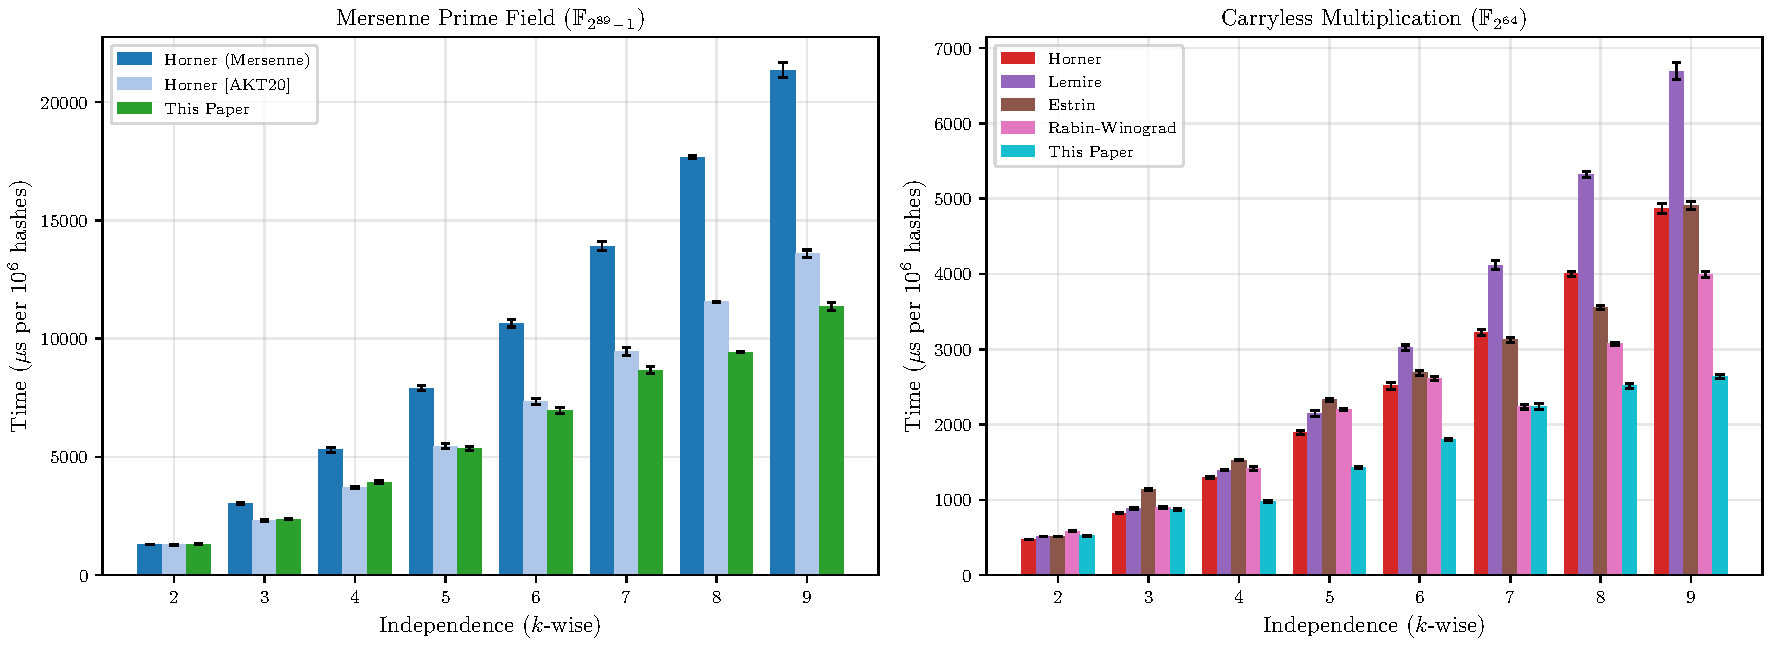
\includegraphics[width=\columnwidth]{figures/bench_all.pdf}
    \caption{Comparison across finite fields: Mersenne prime (left) vs.\
             carryless $\mathbb{F}_{2^{64}}$ (right).
             Carryless multiplication is $3$--$5\times$ faster due to
             hardware support via \texttt{PMULL}/\texttt{PCLMULQDQ}.}
    \label{fig:bench_all}
\end{figure}

Table~\ref{tab:kwise_both} shows the carryless hashing results on both platforms.
Our polynomial chains are the fastest method for most values of $k$, except at $k=7$ where Rabin--Winograd performs best.

\begin{table}[!htbp]
\centering
\caption{$k$-wise carryless hashing (\textmu s per $10^6$ hashes).
         Best method in bold for each platform.}
\label{tab:kwise_both}
\begin{tabular}{c|rrrrr|rrrrr}
    & \multicolumn{5}{c|}{ARM (Apple M1 Pro)} & \multicolumn{5}{c}{x86 (AMD EPYC 9R14)} \\
    $k$ & Horner & Lemire & Estrin & R--W & Ours & Horner & Lemire & Estrin & R--W & Ours \\
    \hline
    3 & 852 & 1144 & 1330 & 1537 & \textbf{914} & 3277 & \textbf{2198} & 3278 & 2281 & 2285 \\
    5 & 1931 & 2911 & 3075 & 3125 & \textbf{1521} & 6558 & 5653 & 6558 & 6140 & \textbf{4214} \\
    7 & 3354 & 5558 & 4002 & \textbf{2346} & 2346 & 10501 & 10005 & 8745 & \textbf{6236} & 6074 \\
    9 & 5188 & 9082 & 5856 & 4716 & \textbf{2833} & 14754 & 14489 & 12546 & 10300 & \textbf{7303} \\
\end{tabular}
\end{table}
For $k = 9$, our method achieves a speedup of $1.83\times$ over Horner on ARM and $2.02\times$ on x86.
For smaller $k$, we use Motzkin's method for $k=4$ (2 multiplications) and direct evaluation for $k=3$ (1 multiplication).
The speedup increases with $k$ because our polynomial chains save more multiplications
at higher degrees: for monic degree $n$, Horner uses $n-1$ multiplications while our
chains use only $\lfloor n/2\rfloor+1$ multiplications (by \cref{thm:main}).

\paragraph{Discussion.}
The Rabin--Winograd method performs best at $k = 7$ where its recursive structure
aligns well with the degree, achieving performance competitive with Estrin.
For other values of $k$, Rabin--Winograd is slower than our method but remains competitive
with standard approaches.
Estrin's scheme provides modest speedup at higher degrees due to its parallelism,
but the additional multiplications limit its effectiveness.
Lemire's reduction is slower than Horner because, on Apple Silicon,
the \texttt{PMULL} instruction is faster than table lookup operations.

Our method achieves the best performance by combining two key insights:
(1) minimizing the number of multiplications through carefully constructed polynomial chains,
and (2) optimizing the implementation to avoid unnecessary data movement between
scalar and vector registers.

On x86 (AMD EPYC 9R14), similar trends hold: our method achieves $2.02\times$ speedup
over Horner at $k=9$ (vs.\ $1.81\times$ on ARM).
Rabin--Winograd is competitive at $k=7$ on both platforms.
Notably, Lemire's table-lookup reduction is faster than Horner on x86,
unlike ARM where \texttt{PMULL} outperforms memory access.

\paragraph{Scope of application benchmarks.}
The remaining experiments measure end-to-end kernels where hashing is only one component.
These are representative workloads rather than an exhaustive study of all data structure designs and microarchitectures.

\subsection{Application-Level Throughput: Sketch Updates}
\label{sec:experiments:sketch}

To check that these savings translate beyond microbenchmarks, we also measure a simple
CountSketch-style update kernel: for each key, compute a hash value, use it to choose a bucket
and a sign bit, and update an array of counters.
This mixes hashing with memory traffic, so speedups are expected to be smaller than in the raw
hash-evaluation benchmark.

With table size $2^{16}$ and $2^{20}$ updates, we measure:
\begin{center}
\begin{tabular}{l|rrr|rrr}
& \multicolumn{3}{c|}{ARM} & \multicolumn{3}{c}{x86} \\
Method & Horner & R--W & Ours & Horner & R--W & Ours \\
\hline
ns/update & 5.49 & 4.96 & \textbf{4.33} & 38.3 & 24.9 & \textbf{23.7}
\end{tabular}
\end{center}
On ARM, our method achieves $1.27\times$ speedup over Horner.
On x86, the speedup is $1.62\times$, reflecting the larger benefit from reducing multiplications.
The benchmark is implemented in \texttt{tools/bench/\allowbreak app\_countsketch\_arm.cpp} (ARM) and
\texttt{tools/bench/\allowbreak app\_countsketch\_x86.cpp} (x86).

\subsection{Application-Level Throughput: Hash Tables}
\label{sec:experiments:hashtable}

Finally, we benchmark a simple linear-probing hash table, measuring both insertion throughput
(table construction) and lookup throughput at load factor $70\%$.
This stresses both hashing and memory probing; as expected, improvements are smaller than the
microbenchmarks, but still measurable.

With table size $2^{20}$, we obtain:
\begin{center}
\begin{tabular}{l|rrr|rrr}
& \multicolumn{3}{c|}{ARM} & \multicolumn{3}{c}{x86} \\
Method & Horner & R--W & Ours & Horner & R--W & Ours \\
\hline
ns/insert & 32.5 & 28.5 & \textbf{28.5} & 37.4 & 29.9 & \textbf{24.5} \\
ns/query  & 42.7 & 41.9 & \textbf{38.6} & 46.3 & 35.4 & \textbf{31.4}
\end{tabular}
\end{center}
On ARM, our method achieves $1.14\times$ speedup for inserts and $1.11\times$ for lookups.
On x86, speedups are larger: $1.53\times$ for inserts and $1.47\times$ for lookups.
The benchmark is implemented in \texttt{tools/bench/\allowbreak app\_linearprobe\_arm.cpp} (ARM) and
\texttt{tools/bench/\allowbreak app\_linearprobe\_x86.cpp} (x86).

\subsection{Application-Level Throughput: Membership Filters}
\label{sec:experiments:filter}

We also implement a simple XOR-filter-style approximate membership structure, which builds a
small fingerprint array using a peeling algorithm and answers queries with three table reads and
two XORs.
We measure both build throughput (ns/key) and query throughput (ns/query) at load $75\%$ and table
size $2^{20}$:
\begin{center}
\begin{tabular}{l|rrr|rrr}
& \multicolumn{3}{c|}{ARM} & \multicolumn{3}{c}{x86} \\
Method & Horner & R--W & Ours & Horner & R--W & Ours \\
\hline
ns/key (build) & 96.1 & \textbf{82.4} & 92.0 & 142.0 & 110.3 & \textbf{97.1} \\
ns/query       & 5.56 & 5.53 & \textbf{5.04} & 19.6 & 15.6 & \textbf{11.1}
\end{tabular}
\end{center}
On ARM, our method improves query throughput by $1.10\times$ over Horner, while R--W is faster at build time.
On x86, our method is fastest for both: $1.46\times$ speedup for build and $1.76\times$ for queries.
The benchmark is implemented in \texttt{tools/bench/\allowbreak app\_xorfilter\_arm.cpp} (ARM) and
\texttt{tools/bench/\allowbreak app\_xorfilter\_x86.cpp} (x86).

\subsection{Cryptographic Workloads: Secret Sharing and Polynomial PRFs}
\label{sec:experiments:crypto}

We also benchmark the same ``evaluate one random polynomial at many points'' inner loop that
appears in threshold secret sharing~\cite{shamir1979share} and related primitives.
To model prime-field arithmetic (where a multiplication is ``full width'' regardless of whether
the input happens to be a small integer), we use the Mersenne prime field
$\F_p$ with $p = 2^{89}-1$ and implement multiplication using 128-bit integer arithmetic and
Mersenne reduction.

We compare Horner evaluation against our ``x2s'' chains (degrees $13,15,17,19,21$ from our search)
in two regimes:
(1) ``Share generation'': evaluation points $x_i = i$ (but treated as elements of $\F_p$, so each
multiply is a full field multiplication), and
(2) ``Polynomial PRF'': evaluation points $x_i \sim \F_p$ uniformly at random.
Both correspond to real cryptographic use cases; the second is also a proxy for polynomial-based
PRFs / universal hashing keyed by the (preprocessed) coefficients.

On an Apple M1 Pro, we observe consistent $2.0\times$--$2.5\times$ speedups over full-field Horner
evaluation for degrees $13$--$21$ in both regimes; see the benchmark implementation in
\texttt{tools/bench/shamir\_sharegen\_mersenne.cpp}.
Including the cost of writing shares to memory gives essentially the same speedups; see
\texttt{tools/bench/shamir\_sharegen\_mersenne\_store.cpp}.

\begin{center}
\begin{tabular}{c|ccccc}
Degree $n$ & 13 & 15 & 17 & 19 & 21 \\
\hline
ARM: Sharegen ($x_i=i$) & 2.02$\times$ & 2.37$\times$ & 2.47$\times$ & 2.49$\times$ & 2.44$\times$ \\
ARM: PRF ($x_i \sim \F_p$) & 2.01$\times$ & 2.34$\times$ & 2.48$\times$ & 2.48$\times$ & 2.48$\times$ \\
\hline
x86: Sharegen ($x_i=i$) & 1.66$\times$ & 4.50$\times$ & 4.57$\times$ & 4.63$\times$ & 4.60$\times$ \\
x86: PRF ($x_i \sim \F_p$) & 1.66$\times$ & 4.50$\times$ & 4.57$\times$ & 4.63$\times$ & 4.60$\times$
\end{tabular}
\end{center}
On x86, the speedups for degrees $15$--$21$ reach $4.5\times$--$4.6\times$, significantly
exceeding the ARM results.

\paragraph{Goldilocks prime field.}
Prime fields of 64-bit size are widely used in proof systems; a common choice is the
``Goldilocks'' prime $p = 2^{64}-2^{32}+1$.
We repeat the same benchmark in $\F_p$ and observe similar improvements:
\begin{center}
\begin{tabular}{c|ccccc}
Degree $n$ & 13 & 15 & 17 & 19 & 21 \\
\hline
ARM: Sharegen ($x_i=i$) & 1.98$\times$ & 2.23$\times$ & 2.39$\times$ & 2.33$\times$ & 2.32$\times$ \\
ARM: PRF ($x_i \sim \F_p$) & 1.96$\times$ & 2.29$\times$ & 2.35$\times$ & 2.34$\times$ & 2.34$\times$ \\
\hline
x86: Sharegen ($x_i=i$) & 1.27$\times$ & 1.38$\times$ & 1.42$\times$ & 1.43$\times$ & 1.37$\times$ \\
x86: PRF ($x_i \sim \F_p$) & 1.27$\times$ & 1.38$\times$ & 1.42$\times$ & 1.43$\times$ & 1.37$\times$
\end{tabular}
\end{center}
The benchmark is implemented in \texttt{tools/bench/\allowbreak app\_goldilocks\_stark\_eval.cpp}.
On ARM, including memory stores gives $2.19\times$--$2.36\times$ speedup;
on x86, the range is $1.31\times$--$1.90\times$.
The smaller x86 gains reflect that Goldilocks multiplication (64-bit) is relatively cheaper,
reducing the benefit of fewer multiplications.
\par\noindent\texttt{tools/bench/\allowbreak app\_goldilocks\_sharegen\_store.cpp} contains the benchmark.

\subsection{Comparison with Tabulation Hashing}

Tabulation hashing~\cite{patracscu2012power} achieves 3-wise independence using
table lookups, providing excellent performance for applications that only require
low independence.
On ARM, simple tabulation (8 tables of 256 entries) achieves
1660$\pm$12\,\textmu s per $10^6$ hashes; on x86, it achieves 6952$\pm$5\,\textmu s.

Notably, our 3-wise independent hash function runs in 914$\pm$4\,\textmu s on ARM---nearly $2\times$ faster than
tabulation with the same independence guarantee.
On x86, our method (2285\,\textmu s) is $3\times$ faster than tabulation.
Our 4-wise hash (using Motzkin's method) is still faster than 3-wise tabulation on both platforms.

\begin{center}
\begin{tabular}{l|rr|rr}
    & \multicolumn{2}{c|}{ARM} & \multicolumn{2}{c}{x86} \\
    Method & Time (\textmu s) & Indep. & Time (\textmu s) & Indep. \\
    \hline
    MurmurHash3 & 593$\pm$8 & none & 1042$\pm$2 & none \\
    xxHash64 & 1174$\pm$5 & none & 1862$\pm$4 & none \\
    Tabulation & 1660$\pm$12 & 3-wise & 6952$\pm$5 & 3-wise \\
    This Paper ($k=3$) & 914$\pm$4 & 3-wise & 2285$\pm$3 & 3-wise \\
    This Paper ($k=4$) & 1036$\pm$13 & 4-wise & 3930$\pm$4 & 4-wise \\
    This Paper ($k=5$) & 1521$\pm$8 & 5-wise & 4214$\pm$3 & 5-wise \\
    This Paper ($k=7$) & 2346$\pm$9 & 7-wise & 6074$\pm$4 & 7-wise \\
\end{tabular}
\end{center}

\subsection{Comparison Across Finite Fields}

We also benchmark polynomial evaluation over the Mersenne prime field
$\mathbb{F}_{2^{89}-1}$, which uses 89-bit integers and standard multiplication
with modular reduction (Figure~\ref{fig:bench_all}).
For the Mersenne baseline, we use the optimized Horner implementation
from Ahle et al.~\cite{ahle2020power}, which employs fast branch-free
modular reduction and delays the final reduction to the end of the computation.
The carryless multiplication methods over $\mathbb{F}_{2^{64}}$ are consistently
$3$--$5\times$ faster than their Mersenne counterparts.
This speedup comes from hardware support for carryless multiplication (via \texttt{PMULL} on Apple M1 Pro),
which computes a 64-bit carryless product directly,
whereas Mersenne arithmetic requires multiple standard multiplications
and careful handling of the 89-bit modulus.

For $k=9$, our method over $\mathbb{F}_{2^{64}}$ (2833\,\textmu s mean) is
$4.2\times$ faster than the best Mersenne method in our benchmark (11864\,\textmu s mean).

\subsection{Injective Polynomial Hashing}
\label{sec:experiments:injective}

We briefly summarize the injective polynomial construction from Section~\ref{sec:injective}
before the comprehensive comparison in Section~\ref{sec:experiments:universal}.
The recurrence
\[
    P_0 = x, \quad P_i = a_i + (b_i + y)(P_{i-1} + x^2)
\]
uses only two random keys $(x, y)$ to hash $2N$ message values $(a_1, b_1, \ldots, a_N, b_N)$
with $N$ multiplications---half the $2N-1$ required by Horner.

\begin{table}[!htbp]
\centering
\caption{Injective vs.\ Horner: $N$ multiplications vs.\ $2N-1$.
         Times in \textmu s per $10^6$ hashes (mean$\pm$std).}
\label{tab:injective}
\begin{tabular}{c|rrr|rrr}
    & \multicolumn{3}{c|}{ARM (Apple M1 Pro)} & \multicolumn{3}{c}{x86 (AMD EPYC 9R14)} \\
    $2N$ & Horner & Injective & Speedup & Horner & Injective & Speedup \\
    \hline
    8  & 5560$\pm$20 & 3960$\pm$30 & $1.40\times$ & 16115$\pm$6 & 13672$\pm$6 & $1.18\times$ \\
    16 & 21030$\pm$160 & 9950$\pm$50 & $2.11\times$ & 48811$\pm$41 & 30413$\pm$9 & $1.61\times$ \\
    32 & 73720$\pm$240 & 40430$\pm$70 & $1.82\times$ & 134847$\pm$15 & 66778$\pm$27 & $2.02\times$ \\
    64 & 226910$\pm$940 & 114960$\pm$350 & $1.97\times$ & 310923$\pm$85 & 165921$\pm$27 & $1.87\times$ \\
\end{tabular}
\end{table}

The speedup approaches $2\times$ as expected from the multiplication count.
On x86, the gains are similar, ranging from $1.18\times$ at $2N=8$ to $2.02\times$ at $2N=32$.
For parallel variants and comparison with other methods (CLNH, BRW, etc.),
see Section~\ref{sec:experiments:universal}.

\subsection{Universal Hashing}
\label{sec:experiments:universal}

Universal hashing uses $O(1)$ random keys to hash variable-length messages.
Unlike $k$-wise hashing where polynomial coefficients are keys,
here the evaluation point(s) are keys and message values form the polynomial.
We compare several constructions, each offering different trade-offs between
key size, multiplication count, and parallelism.

\subsubsection{Horner-based Methods}

The simplest universal hash evaluates the polynomial
$h(x) = m_0 x^{n-1} + m_1 x^{n-2} + \cdots + m_{n-1}$
where $x$ is the random key and $(m_0, \ldots, m_{n-1})$ is the message.

\paragraph{Horner (Sequential).}
Horner's rule computes $h_0 = m_0$, $h_i = h_{i-1} \cdot x + m_i$ for $i = 1, \ldots, n-1$.
This requires $n-1$ multiplications with a \emph{critical path} of $n-1$ dependent operations.
On CPUs where multiplication has multi-cycle latency, this sequential
dependency chain leaves execution units idle.

\paragraph{Horner-Unrolled.}
We process four message values per iteration using Estrin-style grouping:
\[
h \cdot x^4 + (m_i \cdot x + m_{i+1}) \cdot x^2 + (m_{i+2} \cdot x + m_{i+3}).
\]
The terms $(m_i \cdot x + m_{i+1})$ and $(m_{i+2} \cdot x + m_{i+3})$ can be computed
in parallel, exposing instruction-level parallelism (ILP) within each 4-element group.
This reduces effective critical path by $\approx 4\times$ with minimal overhead.

\paragraph{Horner-Parallel.}
Horner's recurrence $h_i = h_{i-1} \cdot x + m_i$ is a linear map with transfer function
$(c, d) = (x, m_i)$, meaning $h \mapsto h \cdot c + d$.
Writing $T_{c,d}(h)\coloneqq h\cdot c + d$, composition is
\[
   T_{c_2,d_2}\!\circ T_{c_1,d_1} = T_{c_1c_2,\; d_1c_2 + d_2}.
\]
Since $c = x$ for all steps, we precompute powers $x, x^2, x^4, \ldots$ and combine
message values in a binary tree with $O(\log n)$ depth.
This requires $O(n)$ total multiplications but only $O(\log n)$ on the critical path.

\subsubsection{Injective Polynomial (This Paper)}

Our injective construction from Section~\ref{sec:injective} uses the recurrence:
\[
P_0 = x, \quad P_i = a_i + (b_i + y)(P_{i-1} + x^2).
\]
The message $(a_1, b_1, \ldots, a_N, b_N)$ has $2N$ values, and the keys are $(x, y)$---just
two field elements regardless of message length.
Each step requires one multiplication (computing $(b_i + y)(P_{i-1} + x^2)$),
so $N$ multiplications hash $2N$ values.
This is nearly $2\times$ fewer than Horner's $2N-1$ multiplications.

\paragraph{Injective-Parallel.}
The recurrence $P_i = a_i + c_i(P_{i-1} + x^2)$ where $c_i = b_i + y$ has transfer functions
$(c_i, d_i)$ with $d_i = a_i + c_i \cdot x^2$.
Unlike Horner, the coefficients $c_i$ vary, so we cannot simply precompute powers.
Instead, we compute all $(c_i, d_i)$ pairs in parallel (Phase~1: $N$ multiplications),
then perform parallel prefix reduction (Phase~2: $2N$ multiplications in $O(\log N)$ depth).
Total work is $3N$ multiplications, but critical path is only $O(\log N)$.

\subsubsection{CLNH (Multilinear Hashing)}

Carry-less NH (CLNH)~\cite{lemire2015clhash} is a multilinear hash:
\[
h = \bigoplus_{i=0}^{N-1} (k_{2i} \oplus m_{2i})(k_{2i+1} \oplus m_{2i+1})
\]
where $(k_0, \ldots, k_{2N-1})$ are random keys and $(m_0, \ldots, m_{2N-1})$ is the message.
All $N$ multiplications are \emph{completely independent}, giving $O(1)$ critical path depth.
This makes CLNH extremely fast on CPUs with multiple execution units.

\paragraph{Trade-off.}
CLNH requires $O(N)$ keys to hash an $N$-word message, compared to $O(1)$ for polynomial methods.
This is acceptable when key material can be generated once and reused (e.g., for a fixed
maximum message length), but problematic for variable-length or streaming applications.
We include CLNH as a performance baseline representing the ``best possible'' when key size
is unconstrained.

\subsubsection{BRW (Bernstein-Rabin-Winograd)}

The BRW construction~\cite{rabin1972number} uses divide-and-conquer to build a polynomial
with optimal $O(\log N)$ depth.
For a message $(m_1, \ldots, m_n)$, the BRW polynomial is defined recursively:
\begin{align}
\text{BRW}(m_1) &= m_1 \\
\text{BRW}(m_1, m_2) &= m_1 \cdot x + m_2 \\
\text{BRW}(m_1, m_2, m_3) &= (x + m_1)(x^2 + m_2) + m_3 \\
\text{BRW}(m_1, \ldots, m_{2^k-1}) &= \text{BRW}(\text{left}) \cdot (x^{2^{k-1}} + m_{2^{k-1}}) + \text{BRW}(\text{right})
\end{align}
This achieves $\approx n/2$ multiplications with $O(\log n)$ depth, which is asymptotically optimal up to lower-order terms~\cite{rabin1972number}.

\paragraph{Practical Limitation.}
Despite theoretical optimality, BRW performs poorly in practice.
The recursive structure with irregular base cases prevents effective compiler optimization.
Function call overhead and unpredictable branching inhibit instruction scheduling,
resulting in slower execution than simpler iterative methods.

\subsubsection{c-Decimated BRW}

To improve BRW's practical performance, $c$-decimated BRW splits the message into
$c$ interleaved streams, applies BRW to each stream, and combines results:
\[
h = \text{BRW}(m_0, m_c, m_{2c}, \ldots) + x^d \cdot \text{BRW}(m_1, m_{c+1}, \ldots) + \cdots
\]
where $d$ is chosen to avoid coefficient collisions.
The $c$ independent BRW evaluations can execute in parallel, improving ILP.
We benchmark $c = 2$ and $c = 4$.

\paragraph{Result.}
Even with decimation, BRW variants remain slower than Horner-Unrolled and Injective-Parallel.
The recursive structure still prevents optimal code generation.

\subsubsection{Comprehensive Comparison}
Table~\ref{tab:universal_full} compares all methods across message sizes.
Times are in \textmu s per $10^5$ hashes, shown as mean$\pm$std over 50 runs.

\begin{table}[!htbp]
\centering
\caption{Universal hashing comparison (\textmu s per $10^5$ hashes).
         CLNH uses $O(N)$ keys; all others use $O(1)$ keys.
         Best $O(1)$-key method in bold.}
\label{tab:universal_full}
\resizebox{\columnwidth}{!}{%
\begin{tabular}{c|rrr|rr|r|rrr}
    & \multicolumn{3}{c|}{Horner variants} & \multicolumn{2}{c|}{Injective} & CLNH & \multicolumn{3}{c}{BRW variants} \\
    $2N$ & Seq & Unroll & Par & Seq & Par & & BRW & 2-dec & 4-dec \\
    \hline
    8   & 556$\pm$2 & 465$\pm$0 & 2475$\pm$14 & \textbf{396$\pm$3} & 831$\pm$7 & 185$\pm$1 & 1233$\pm$12 & 1449$\pm$13 & 405$\pm$2 \\
    16  & 2103$\pm$16 & 1048$\pm$8 & 3483$\pm$46 & \textbf{995$\pm$5} & 1552$\pm$5 & 348$\pm$2 & 2337$\pm$18 & 2505$\pm$18 & 3116$\pm$10 \\
    32  & 7372$\pm$24 & 2710$\pm$15 & 6681$\pm$109 & 4043$\pm$7 & \textbf{2710$\pm$16} & 1078$\pm$13 & 4511$\pm$25 & 4690$\pm$26 & 5845$\pm$27 \\
    64  & 22691$\pm$94 & 6648$\pm$23 & 13053$\pm$179 & 11496$\pm$35 & \textbf{5166$\pm$25} & 2119$\pm$11 & 8872$\pm$45 & 10949$\pm$44 & 10309$\pm$52 \\
    128 & 64521$\pm$313 & 13662$\pm$83 & 22687$\pm$516 & 27862$\pm$442 & \textbf{10294$\pm$66} & 4225$\pm$19 & 17682$\pm$150 & 23764$\pm$290 & 20756$\pm$150 \\
    256 & 147845$\pm$793 & 34238$\pm$95 & 21313$\pm$225 & 71052$\pm$369 & \textbf{21619$\pm$131} & 8869$\pm$53 & 35177$\pm$347 & 39859$\pm$337 & 47505$\pm$8187 \\
\end{tabular}
}
\end{table}

\paragraph{Key Observations.}
\begin{enumerate}
    \item \textbf{CLNH is fastest} but uses $O(N)$ keys---suitable when key material is not a constraint.
    \item For \textbf{$O(1)$-key methods}:
    \begin{itemize}
        \item \textbf{Small messages ($2N \le 16$)}: Sequential Injective wins due to minimal overhead
              and half the multiplications of Horner.
        \item \textbf{Large messages ($2N \ge 32$)}: Injective-Parallel wins by exploiting ILP.
              At $2N = 256$, it achieves $6.8\times$ speedup over sequential Horner.
        \item Horner-Unrolled is a good middle ground: simple to implement, $4.3\times$ faster than Horner.
    \end{itemize}
    \item \textbf{BRW underperforms} despite optimal $O(\log N)$ depth.
          The recursive structure prevents effective compiler optimization.
          c-decimated BRW variants are similarly slow.
    \item \textbf{Horner-Parallel} shows non-monotonic behavior: $2N = 256$ is slightly faster than
          $2N = 128$ in wall-clock time, likely due to better instruction scheduling at that
          specific unrolled size. The $O(\log N)$ depth advantage becomes apparent at large $N$.
\end{enumerate}

\paragraph{Parallelization Strategy.}
The injective recurrence $P_i = a_i + c_i \cdot (P_{i-1} + x^2)$ where $c_i = b_i + y$
can be expressed as transfer functions $(c_i, d_i)$ where $d_i = a_i + c_i \cdot x^2$.
With $T_{c,d}(h)\coloneqq h\cdot c + d$, the same composition rule applies:
$T_{c_2,d_2}\!\circ T_{c_1,d_1} = T_{c_1c_2,\; d_1c_2 + d_2}$.
We compute all $(c_i, d_i)$ pairs in parallel (Phase~1), then combine them with
parallel prefix scan (Phase~2), achieving $O(\log N)$ critical path depth.

Unlike Horner where $c = x$ for all steps (allowing power precomputation),
the injective recurrence has varying $c_i$, requiring $3N$ multiplications total.
Despite $3\times$ more work than sequential ($N$ multiplications),
Injective-Parallel is $3.3\times$ faster at $2N = 256$ because Apple M1 can
execute multiple independent \texttt{PMULL} instructions per cycle.

\subsection{Implementation Insights}
\label{sec:experiments:implementation}

Our benchmarks reveal several microarchitectural insights for polynomial evaluation
on Apple M1 Pro (and, qualitatively, on other out-of-order CPUs with carryless multiplication):

\paragraph{Latency vs.\ Throughput.}
The \texttt{PMULL} instruction on Apple M1 has $\approx 3$ cycle latency but the
processor can issue multiple independent \texttt{PMULL}s per cycle.
Sequential algorithms like Horner are \emph{latency-bound}: each multiplication
depends on the previous result, leaving execution units idle.
Parallel algorithms like our prefix scan are \emph{throughput-bound}: they generate
enough independent work to keep all units busy.

For message length $2N=256$, sequential Horner has a critical path of $255$ dependent multiplications,
while Injective-Parallel has only $O(\log N)$ levels of dependent multiplications (about 8 levels for $N=128$),
plus parallel work at each level.

\paragraph{Compiler Optimization.}
The effectiveness of parallelism depends heavily on compiler optimization.
Our Injective-Parallel implementation uses simple loops that the compiler
fully unrolls and interleaves, generating dense streams of independent \texttt{PMULL}
instructions.
In contrast, recursive algorithms like BRW (Bernstein-Rabin-Winograd) suffer from
function call overhead and irregular control flow that inhibit optimization.

At $2N = 256$, Injective-Parallel ($21619 \pm 131$\,\textmu s) outperforms BRW ($35177 \pm 347$\,\textmu s)
by $1.6\times$ despite BRW having theoretically optimal $O(\log N)$ depth,
because the iterative structure admits better code generation.

\paragraph{Memory Layout.}
Storing keys as scalar 64-bit integers rather than 128-bit SIMD vectors improves
performance by $10$--$15\%$ on Apple Silicon.
This allows XOR operations to use the faster scalar ALU, and reduces register pressure
when many coefficients are live simultaneously during tree reductions.

\section{Open Problems}
\label{sec:open-problems}

\paragraph{Constructions for characteristic 2.}
Our main construction relies on the identity $(a+b)^2 = a^2 + 2ab + b^2$, which fails in characteristic 2 since $2ab = 0$.
While we provide some characteristic-2 constructions in the appendix, a general construction achieving $\lfloor n/2 \rfloor + O(1)$ multiplications for all degrees remains open.

\paragraph{Lower bounds for characteristic 2.}
Our lower bound proof uses properties specific to fields of characteristic $\neq 2$.
Does the same $\lfloor n/2 \rfloor + 1$ lower bound hold in characteristic 2, or can one do better?

\bibliographystyle{alpha}
\bibliography{references}  % references.bib
\appendix
\section{Optimized Polynomial Circuits}\label{appendix:polynomials}

This appendix records optimized candidate circuits with four through eleven
multiplication gates.  A circuit with $m$ products below has $2m-1$ keys and
outputs a monic polynomial of degree $2m-1$.  The circuits were found by
randomized search, optimizing both the number of additions and the critical
path depth.  Explicit inverses are proved below for the displayed characteristic-$2$
circuits of degrees $7$, $15$, $17$, $19$, and $21$, and for separately displayed
alternatives of degrees $9$, $11$, and $13$.  The other search results are not used in
the proof of the main theorem.  In particular, a constant nonzero Jacobian found
by the search is only a diagnostic (and a necessary condition for a
polynomial automorphism), not a proof of bijectivity.

\subsection{Characteristic 2 (\texorpdfstring{$\F_{2^{64}}$}{GF(2\^{}64)})}

Each circuit computes a polynomial $P(x)$ over $\F_{2^{64}}$ using carryless multiplications,
parameterized by keys $a_0, a_1, \ldots$.
All additions are XOR, and each multiplication uses Galois field reduction.
Timings are medians over $10^6$ random inputs on an Apple M2 Pro using ARM NEON
\texttt{PMULL} (\texttt{tools/bench/appendix\_char2\_circuits\_arm.cpp}).

\medskip
\noindent
\begin{minipage}[t]{0.47\textwidth}
\textbf{4 products, degree 7} (7 keys)
\[
\begin{aligned}
y &= (x + 0)(x + a_0) \\
z &= (x + a_1)(y + a_2) \\
t &= (x + y + z + a_3) \\
  &\quad\cdot(x + y + z + 0) \\
u &= (x + a_4)(y + t + a_5) \\
P &= u + a_6
\end{aligned}
\]
\emph{2.3 ns, h=4, 12 XORs}
\end{minipage}
\hfill
\begin{minipage}[t]{0.47\textwidth}
\textbf{5 products, degree 9} (9 keys)
\[
\begin{aligned}
y &= (x + 0)(x + 0) \\
z &= (x + y + a_0)(x + a_1) \\
t &= (z + a_2)(y + z + a_3) \\
u &= (x + z + t + a_4) \\
  &\quad\cdot(x + y + z + a_5) \\
v &= (x + a_6)(y + a_7) \\
P &= u + v + a_8
\end{aligned}
\]
\emph{3.1 ns, h=4, 16 XORs}
\end{minipage}

\begin{lemma}[Direct inverse for the first characteristic-2 circuit]\label{lem:first-char2-circuit-inverse}
Let $\F$ be a perfect field of characteristic $2$, for example $\F_{2^{64}}$.
Fix distinct $x_0,\ldots,x_6\in\F$.
For the first circuit above, the map
\[
    (a_0,\ldots,a_6)
        \longmapsto
    \bigl(P_{a_0,\ldots,a_6}(x_0),\ldots,P_{a_0,\ldots,a_6}(x_6)\bigr)
\]
is a bijection $\F^7\to\F^7$.
\end{lemma}
\begin{proof}
Given values $v_i=P(x_i)$, first recover the coefficients $p_0,\ldots,p_6$ of the unique monic degree-$7$ polynomial
\[
    P(x)=x^7+\sum_{j=0}^6 p_jx^j
\]
with $P(x_i)=v_i$.
Equivalently, solve the Vandermonde system
\[
    \sum_{j=0}^6 p_jx_i^j = v_i+x_i^7,
    \qquad i=0,\ldots,6.
\]
The system is invertible because the $x_i$ are distinct.

We now recover the keys from the $p_j$.
Since the square map is bijective over $\F$, write $r^{1/2}$ for the unique square root of $r$.
Set
\[
\begin{aligned}
    a_4 &= p_6,\\
    b &= p_5^{1/2},\\
    a_3 &= p_4+a_4p_5,\\
    c &= \bigl(p_3+a_3b+1+a_4a_3\bigr)^{1/2},\\
    a_0 &= p_2+a_3c+a_4(c^2+a_3b+1),\\
    a_1 &= b+1+a_0,\\
    a_2 &= c+1+a_0+a_0a_1,\\
    d &= a_1a_2,\\
    a_5 &= p_1+d^2+a_3d+a_4(a_3c+a_0),\\
    a_6 &= p_0+a_4(d^2+a_3d+a_5).
\end{aligned}
\]
To verify these formulas, define
\[
    b=1+a_0+a_1,\qquad
    c=1+a_0+a_2+a_0a_1,\qquad
    d=a_1a_2.
\]
Then
\[
    x+y+z=x^3+bx^2+cx+d.
\]
Using characteristic $2$,
\[
    t=(x+y+z+a_3)(x+y+z)=(x+y+z)^2+a_3(x+y+z),
\]
and hence
\[
    y+t+a_5
    =x^6+b^2x^4+a_3x^3+(c^2+a_3b+1)x^2+(a_3c+a_0)x+(d^2+a_3d+a_5).
\]
Multiplying by $x+a_4$ and adding $a_6$ gives
\[
\begin{aligned}
    p_6 &= a_4,\\
    p_5 &= b^2,\\
    p_4 &= a_3+a_4b^2,\\
    p_3 &= c^2+a_3b+1+a_4a_3,\\
    p_2 &= a_3c+a_0+a_4(c^2+a_3b+1),\\
    p_1 &= d^2+a_3d+a_5+a_4(a_3c+a_0),\\
    p_0 &= a_4(d^2+a_3d+a_5)+a_6.
\end{aligned}
\]
The displayed recovery procedure solves these equations in order, so it recovers a unique key tuple.
Conversely, applying the recovered keys gives the same coefficients $p_j$, hence the same values at the $x_i$.
\end{proof}

\medskip
\noindent
\begin{minipage}[t]{0.47\textwidth}
\textbf{6 products, degree 11} (11 keys)
\[
\begin{aligned}
y &= (x + 0)(x + a_0) \\
z &= (x + y + a_1)(x + y + 0) \\
t &= (x + z + a_2)(z + a_3) \\
u &= (t + a_4)(x + a_5) \\
v &= (x + y + z + t + u + a_6) \\
  &\quad\cdot(y + a_7) \\
w &= (x + a_8)(y + z + t + a_9) \\
P &= z + v + w + a_{10}
\end{aligned}
\]
\emph{4.4 ns, h=5, 22 XORs}
\end{minipage}
\hfill
\begin{minipage}[t]{0.47\textwidth}
\textbf{7 products, degree 13} (13 keys)
\[
\begin{aligned}
y &= (x + 0)(x + 0) \\
z &= (y + a_0)(x + y + a_1) \\
t &= (x + z + a_2)(x + a_3) \\
u &= (x + y + a_4)(x + t + a_5) \\
v &= (y + z + a_6)(u + a_7) \\
w &= (y + z + t + a_8) \\
  &\quad\cdot(x + u + a_9) \\
s &= (x + z + u + v + w + a_{10}) \\
  &\quad\cdot(x + a_{11}) \\
P &= t + s + a_{12}
\end{aligned}
\]
\emph{5.5 ns, h=6, 26 XORs}
\end{minipage}

\medskip
\noindent
The three benchmarked circuits above are retained as search candidates.  For
the proofs, we use the following separately optimized alternatives; unlike the
candidate circuits, each comes with the explicit inverse below.
\[
\begin{array}{c|l}
9 &
\begin{aligned}
y&=x(x+a_0),& z&=x(y+a_1),& t&=(y+z+a_2)(z+a_3),\\
u&=(x+z+a_4)(t+a_5),& v&=(y+a_6)(z+a_7),& P&=u+v+a_8;
\end{aligned}\\[2ex]
11 &
\begin{aligned}
y&=x(x+a_0),& z&=(y+a_1)(x+y+a_2),& t&=x(y+a_3),\\
u&=(t+a_4)(z+a_5),&v&=(x+y+t+u+a_6)(z+t+a_7),\\
w&=(t+a_8)(y+u+a_9),&P&=v+w+a_{10};
\end{aligned}\\[2ex]
13 &
\begin{aligned}
y&=x^2,&z&=(x+y+a_{12})(y+a_{11}),&w&=(y+z+a_{10})(z+a_9),\\
v&=(y+z+a_8)(w+a_7),&u&=(z+v+a_6)(x+a_5),\\
t&=(x+y+a_4)(x+a_3),&s&=(w+t+a_2)(y+a_1),&P&=u+v+s+a_0.
\end{aligned}
\end{array}                                                     \tag{A.0}
\]
Their respective $(\text{height},\text{XOR count})$ pairs are
$(4,12)$, $(4,18)$, and $(5,21)$; these alternatives were not included in
the timing run quoted above.

\begin{lemma}[Explicit inverses for the degree-$9$ and degree-$11$ circuits]
\label{lem:char2-small-staircase-butterfly}
Over every field of characteristic $2$, the coefficient map of the displayed
degree-$9$ circuit is a polynomial bijection.  Over every perfect field of
characteristic $2$, the coefficient map of the displayed degree-$11$ circuit is
a bijection.  Consequently their evaluation maps at respectively nine and
eleven distinct points are bijections.
\end{lemma}
\begin{proof}
We give the inverse maps.  This also makes clear where perfectness is used.

For degree $9$, write
\(P=x^9+\sum_{j=0}^8c_jx^j\), and first set
\[
\begin{aligned}
 a_0&=c_8+1,\\
 a_1&=c_7+1+a_0+a_0^2,\\
 r&=c_6+1+a_0^2+a_0^3,\\
 s&=c_5+1+a_0^2+a_0^3+a_0^2a_1+a_1^2,\\
 q&=c_4+a_0^2+a_0^2r+a_0a_1^2+a_1+a_1^2.
\end{aligned}                                                    \tag{9.1}
\]
Expanding the first four products gives the constant block
\[
 r=a_2+a_3+a_4,\qquad s=a_3+a_4,\qquad q=a_2+a_3.
\]
Its inverse is
\[
 a_2=r+s,\qquad a_3=q+a_2,\qquad a_4=s+a_3.             \tag{9.2}
\]
Let $B$ be the output of the same circuit after setting
$a_5=a_6=a_7=a_8=0$, with the recovered $a_0,\ldots,a_4$ left in place,
and write $b_j=[x^j]B$.  The remaining descent is
\[
\begin{aligned}
 h&=c_3+b_3,\\
 a_7&=c_2+b_2+a_0h,\\
 a_5&=c_1+b_1+a_1h+a_0a_7,\\
 a_6&=h+a_5,\\
 a_8&=c_0+b_0+a_4a_5+a_6a_7.
\end{aligned}                                                    \tag{9.3}
\]
Indeed, after subtracting the baseline, rows $3,2,1,0$ are respectively
\[
 a_5+a_6,\quad
 a_7+a_0(a_5+a_6),\quad
 a_5+a_1(a_5+a_6)+a_0a_7,\quad
 a_8+a_4a_5+a_6a_7.
\]
Thus every step in (9.1)--(9.3) has unit slope; no root or division is used.

For degree $11$, write
\(P=x^{11}+\sum_{j=0}^{10}c_jx^j\), and put
\[
 a_0=c_{10},\qquad a_3=c_9+1,\qquad a_4=c_8+a_0,
 \qquad s=a_1+a_2,qquad h=a_5+a_7+a_8.
\]
Define the already-known expressions
\[
\begin{aligned}
 K_7&=1+a_0^2+a_0^4+a_3,\\
 K_6&=1+a_0+a_0^3+a_0^5+a_4,\\
 K_5&=a_0+a_0^2+a_0^4a_3+a_0^2a_3+a_3.
\end{aligned}
\]
The next three rows are
\[
\begin{aligned}
 c_7&=K_7+s^2+h,\\
 c_6&=K_6+a_0s^2+(a_0+1)h,\\
 c_5&=K_5+a_0^2(s^2+h)+s+a_1^2+a_3s^2+sh+a_3h.
\end{aligned}                                                    \tag{11.1}
\]
Since the field is perfect, Frobenius is invertible.  Hence
\[
\begin{aligned}
 r&=c_7+K_7,\\
 h&=c_6+K_6+a_0r,\\
 s&=(r+h)^{1/2},\\
 a_1&=\bigl(c_5+K_5+a_0^2r+s+a_3s^2+sh+a_3h\bigr)^{1/2},\\
 a_2&=s+a_1.
\end{aligned}                                                    \tag{11.2}
\]
To expose the lower butterfly, let $B_0$ be the circuit output with
\[
 (a_5,a_6,a_7,a_8,a_9,a_{10})=(0,0,0,h,0,0).
\]
Then $a_6=c_4+[x^4]B_0$.  Recompute this baseline with the recovered $a_6$
in place and call it $B$; put $d_j=c_j+[x^j]B$.  A direct cancellation of
the two final branches gives
\[
 P+B=\kappa(t+a_4)+a_5y+a_7(x+t+a_6)+a_9(t+a_8)+a_{10},
 \quad
 \kappa=a_5(h+a_5),\quad a_8=h+a_5+a_7.              \tag{11.3}
\]
Consequently
\[
\begin{aligned}
 a_5&=d_2+a_0d_3,\\
 \kappa&=a_5(h+a_5),\\
 a_7&=d_1+a_3d_3+a_0a_5,\\
 a_9&=d_3+\kappa+a_7,\\
 a_8&=h+a_5+a_7,\\
 a_{10}&=d_0+\kappa a_4+a_7a_6+a_9a_8.
\end{aligned}                                                    \tag{11.4}
\]
This recovers all eleven keys.  The only non-polynomial-looking operations are
the two inverse-Frobenius steps in (11.2), and these are unique over a perfect
field.

In either degree, evaluation at distinct points is the coefficient map followed
by the corresponding invertible Vandermonde map.
\end{proof}

\begin{lemma}[Unitriangular inverse for the degree-$13$ circuit]
\label{lem:char2-degree13-inverse}
Over every field of characteristic $2$, the coefficient map of the displayed
degree-$13$ circuit is a polynomial bijection.  Consequently its evaluation
map at any thirteen distinct points is a bijection.
\end{lemma}
\begin{proof}
Make the invertible linear change of key coordinates
\[
\begin{aligned}
(q_0,\ldots,q_{12})={}&(a_5, a_{11}+a_{12}, a_{12}, a_9, a_8, a_{10},
 a_1,\\
&a_7, a_3, a_4, a_6, a_2, a_0),
\end{aligned}                                                    \tag{13.1}
\]
and order the coefficient rows as
\[
 (d_0,\ldots,d_{12})=(12,11,10,7,6,9,8,5,4,3,1,2,0).
                                                               \tag{13.2}
\]
After expressing the original keys through (13.1), define the explicit
baseline
\[
 K_i(q_0,\ldots,q_{i-1})
   =[x^{d_i}]P(q_0,\ldots,q_{i-1},0,\ldots,0).
                                                               \tag{13.3}
\]
The seven gate identities give the following unitriangular certificate:
\[
 [x^{d_i}]P=q_i+K_i(q_0,\ldots,q_{i-1})qquad(0\le i\le12).
                                                               \tag{13.4}
\]
For reference, its complete pivot table is
\[
\begin{array}{c|rrrrrrrrrrrrr}
i&0&1&2&3&4&5&6&7&8&9&10&11&12\\ \hline
d_i&12&11&10&7&6&9&8&5&4&3&1&2&0\\
q_i&a_5&a_{11}{+}a_{12}&a_{12}&a_9&a_8&a_{10}&a_1&a_7&a_3&a_4&a_6&a_2&a_0
\end{array}                                                     \tag{13.5}
\]
The first three rows, for example, are
\[
 [x^{12}]P=q_0,\qquad [x^{11}]P=q_0+q_1,
 \qquad [x^{10}]P=1+q_0+q_0q_1+q_2.
\]
We record the only coupled cancellation behind the nonmonotone middle of
(13.5).  If
\[
 W_p=(A+p)B,\qquad V_t=(A+t)(W_p+\ell),\qquad
 F_{p,t}=RV_t+SW_p+E,
\]
then characteristic $2$ gives the literal identity
\[
 F_{p,t}+F_{0,0}
  =(p+t)RAB+ptRB+tR\ell+pSB.                         \tag{13.6}
\]
In the circuit take
\[
 A=z+y,\quad B=z+a_9,\quad R=x+a_5+1,\quad S=y+a_1,\quad
 p=a_{10},\quad t=a_8,\quad \ell=a_7.
\]
The row-$6$ coefficients of both $RAB$ and $SB$ are $1$, so their $p$
terms cancel: row $6$ exposes $a_8$.  Row $9$ then exposes $a_{10}$, and
row $5$ exposes $a_7$.  The remaining entries of (13.5) are the ordinary
unit offsets in unequal-degree factors; their later offsets lie strictly
below the indicated row.  This proves (13.4) without a Jacobian argument.

The inverse is now the explicit recurrence
\[
 q_i=[x^{d_i}]P+K_i(q_0,\ldots,q_{i-1})qquad(0\le i\le12),
\]
followed by the inverse of (13.1).  It uses only addition and multiplication,
so it works over every characteristic-$2$ field.  The evaluation claim again
follows from Vandermonde interpolation.
\end{proof}

\medskip
\noindent
\begin{minipage}[t]{\textwidth}
\textbf{8 products, degree 15} (15 keys)
\[
\begin{aligned}
y &= x^2, \\
z &= (y+a_0)(x+y+a_1), \\
t &= (x+a_2)(z+a_3), \\
u &= (y+t+a_4)(z+t+a_5), \\
v &= (x+z+a_6)(z+a_7), \\
w &= (x+y+z+a_8)(y+v+a_9), \\
s &= (z+a_{10})(v+a_{11}), \\
r &= (t+a_{12})(u+a_{13}), \\
P &= w+s+r+a_{14}.
\end{aligned}
\]
\emph{$h=5$, 24 XORs}
\end{minipage}

\smallskip
\noindent
The next decoder is unitriangular: like those of degrees $19$ and $21$ below,
and unlike the degree-$7$ and degree-$17$ decoders, it requires no Frobenius
roots.

\begin{lemma}[Uniform inverse for the degree-$15$ characteristic-$2$ circuit]
\label{lem:char2-degree15-inverse}
Let $\F$ be any field of characteristic $2$.  The coefficient map of
the displayed degree-$15$ circuit is a bijection from $\F^{15}$ to the monic
degree-$15$ polynomials.  Consequently, for any fifteen distinct
$x_0,\ldots,x_{14}\in\F$, its evaluation map at those points is a bijection
$\F^{15}\to\F^{15}$.
\end{lemma}
\begin{proof}
Write $P=x^{15}+\sum_{j=0}^{14}c_jx^j$.  Replace the gate offsets by the
following invertible linear coordinates:
\[
\begin{array}{lll}
q_0=a_2, & q_1=a_0+a_1, & q_2=a_0,\\
q_3=a_3, & q_4=a_4+a_5+a_{12}, & q_5=a_5,\\
q_6=a_8+a_{10}, & q_7=a_{12}, & q_8=a_6+a_7,\\
q_9=a_{13}, & q_{10}=a_9+a_{11}, & q_{11}=a_7,\\
q_{12}=a_9+a_{10}, & q_{13}=a_9, & q_{14}=a_{14}.
\end{array}                                                       \tag{A.1}
\]
For reference, its inverse is
\[
\begin{array}{lll}
a_0=q_2, & a_1=q_1+q_2, & a_2=q_0,\\
a_3=q_3, & a_4=q_4+q_5+q_7, & a_5=q_5,\\
a_6=q_8+q_{11}, & a_7=q_{11},
  & a_8=q_6+q_{12}+q_{13},\\
a_9=q_{13}, & a_{10}=q_{12}+q_{13},
  & a_{11}=q_{10}+q_{13},\\
a_{12}=q_7, & a_{13}=q_9, & a_{14}=q_{14}.
\end{array}                                                       \tag{A.2}\label{eq:char2-15-q-inverse}
\]

Let $\mathcal P(\mathbf q)$ denote the circuit after the substitution
\eqref{eq:char2-15-q-inverse}.  For $0\le i\le14$, define the explicitly
evaluable baseline
\[
 K_i(q_0,\ldots,q_{i-1})
 =\coeff{\mathcal P(q_0,\ldots,q_{i-1},0,\ldots,0)}{14-i}.
                                                                    \tag{A.3}\label{eq:char2-15-baseline}
\]
Collecting coefficients in the nine displayed assignments gives the
unitriangular identities
\[
 \coeff{\mathcal P(\mathbf q)}{14-i}
   =q_i+K_i(q_0,\ldots,q_{i-1})
   \qquad(0\le i\le14).                                           \tag{A.4}\label{eq:char2-15-triangular}
\]
Here is a compact certificate for the collection: it records the branch in
which each new pivot first survives after the preceding rows have been
removed.
\[
\begin{gathered}
\begin{array}{c|rrrrrrrr}
\text{row}&14&13&12&11&10&9&8&7\\ \hline
\text{pivot}&q_0&q_1&q_2&q_3&q_4&q_5&q_6&q_7\\
\text{branch}&r&r&r&r&r&r&w+s&r
\end{array}\\[3pt]
\begin{array}{c|rrrrrrr}
\text{row}&6&5&4&3&2&1&0\\ \hline
\text{pivot}&q_8&q_9&q_{10}&q_{11}&q_{12}&q_{13}&q_{14}\\
\text{branch}&w+s&r&w+s&w+s&w+s&w+s&\mathrm{out}
\end{array}
\end{gathered}                                                    \tag{A.5}\label{eq:char2-15-pivot-table}
\]
The two cancellations responsible for the alternating lower rows are
\[
\begin{aligned}
u&=t^2+(y+z+a_4+a_5)t+(y+a_4)(z+a_5),\\
w+s&=(x+y+a_8+a_{10})v
 +(x+y+z+a_8)(y+a_9)+(z+a_{10})a_{11}.
\end{aligned}                                                     \tag{A.6}
\]
Thus the common $zv$ term disappears from $w+s$; the remaining products have
distinct degrees.  Descending through the rows in
\eqref{eq:char2-15-pivot-table}, the displayed
factor degrees give the named pivot with slope one, while every other term
contains only coordinates from an earlier column.  This proves
\eqref{eq:char2-15-triangular}
without any nonzero-slope or field-size assumption.

The inverse is now literal.  For $i=0,\ldots,14$, successively set
\[
 q_i=c_{14-i}+K_i(q_0,\ldots,q_{i-1}),                            \tag{A.7}\label{eq:char2-15-decoder}
\]
and then recover the original offsets from
\eqref{eq:char2-15-q-inverse}.  Equations
\eqref{eq:char2-15-triangular} and \eqref{eq:char2-15-decoder} are mutually
inverse polynomial maps, so the
coefficient map is a polynomial automorphism over every characteristic-$2$
field.  Finally, evaluation at fifteen distinct points is an invertible
Vandermonde transformation of the fifteen nonleading coefficients.
\end{proof}

\medskip
\noindent
\begin{minipage}[t]{\textwidth}
\textbf{9 products, degree 17} (17 keys)
\[
\begin{aligned}
y &= x(x+a_0),\\
z &= (x+a_1)(x+y+a_2),\\
t &= (y+a_3)(x+y+a_4),\\
u &= (y+z+a_5)(z+t+a_6),\\
v &= (x+z+a_7)(x+z+t+u+a_8),\\
h &= (y+a_9)x,\\
j &= (y+a_{10})(x+a_{11}),\\
\ell &= (t+a_{12})(h+a_{13}),\\
w &= (x+u+a_{14})(u+v+a_{15}),\\
P &= j+\ell+w+a_{16}.
\end{aligned}
\]
\emph{$h=5$, 29 XORs}
\end{minipage}

\begin{lemma}[Uniform inverse for the degree-$17$ characteristic-$2$ circuit]
\label{lem:char2-degree17-inverse}
Let $\F$ be a perfect field of characteristic $2$.  The coefficient map of
the displayed degree-$17$ circuit is a bijection from $\F^{17}$ to the monic
degree-$17$ polynomials.  Consequently, for any seventeen distinct
$x_0,\ldots,x_{16}\in\F$, its evaluation map at those points is a bijection
$\F^{17}\to\F^{17}$.
\end{lemma}
\begin{proof}
Write $[f]_i=[x^i]f$.  We first replace the gate offsets by normalized gate
coordinates
\[
\begin{aligned}
q_0&=[y]_1,
&(q_1,q_2)&=([z]_2,[z]_1),
&(q_3,q_4)&=([t]_2,[t]_1),\\
(q_5,q_6)&=([u]_4,[u]_3),
&(q_7,q_8)&=([v]_7,[v]_3),
&q_9&=[h]_1,\\
(q_{10},q_{11})&=([j]_2,[j]_1),
&(q_{12},q_{13})&=([\ell]_4,[\ell]_3),
&(q_{14},q_{15})&=([w]_{10},[w]_7),
\end{aligned}                                                     \tag{A.8}
\]
and $q_{16}=a_{16}$.  These are polynomial coordinates on the original
keys.  Indeed, the first three gates give
\[
\begin{aligned}
a_0&=q_0,\\
a_1&=q_1+q_0+1,
&a_2&=q_2+(q_0+1)a_1,\\
\sigma&=q_3+q_0^2+q_0,
&a_3&=q_4+q_0\sigma,
&a_4&=\sigma+a_3.
\end{aligned}                                                     \tag{A.9}
\]
For every remaining two-offset gate use the following unit-pivot identity.
If $A,B$ are already known and monic, $0<\deg A<\deg B$, and
$G=(A+\alpha)(B+\beta)$, then
\[
 \alpha=[G]_{\deg B}+[AB]_{\deg B},\qquad
 \beta=[G]_{\deg A}+[AB+\alpha B]_{\deg A}.                     \tag{A.10}
\]
It applies successively to $u,v,j,\ell,w$ (placing the lower-degree factor
first); also $a_9=q_9$.  Thus (A.8)--(A.10) explicitly recover every
$a_i$ from the $q_i$, without division or a nonvanishing hypothesis.

Now make the elementary coordinate change
\[
 s=q_0+q_3,\qquad r=q_5+q_7,\qquad e=q_4+q_5^2+q_5,               \tag{A.11}
\]
and order the resulting coordinates as
\[
\begin{aligned}
(z_1,\ldots,z_{17})={}&
(q_1,q_2,s,r,q_0,e,q_{14},q_6,q_5,q_{15},\\
&\hspace{34mm}q_8,q_9,q_{12},q_{13},q_{10},q_{11},q_{16}).
\end{aligned}                                                     \tag{A.12}
\]
This change is polynomially invertible:
$q_3=s+q_0$, $q_7=r+q_5$, and $q_4=e+q_5^2+q_5$.

We record the coefficient calculation in a form that is both compact and an
explicit decoder.  For each $i$, let $P_i$ be the output of the same displayed
circuit after retaining $z_1,\ldots,z_{i-1}$ and setting
$z_i,\ldots,z_{17}$ to zero; its original keys are obtained explicitly from
(A.9)--(A.12).  If $P=x^{17}+\sum_{d=0}^{16}c_dx^d$, direct collection of
the indicated rows gives
\[
\begin{array}{c|c|c@{\qquad\qquad}c|c|c}
i&d_i&c_{d_i}+[P_i]_{d_i}&i&d_i&c_{d_i}+[P_i]_{d_i}\\ \hline
1&16&z_1   &10&7&z_{10}\\
2&15&z_2   &11&6&z_{11}\\
3&13&z_3^2 &12&5&z_{12}\\
4&14&z_4   &13&4&z_{13}\\
5&12&z_5   &14&3&z_{14}\\
6&11&z_6   &15&2&z_{15}\\
7&10&z_7   &16&1&z_{16}\\
8&9 &z_8^2 &17&0&z_{17}\\
9&8 &z_9^4 &&&
\end{array}                                                       \tag{A.13}
\]
For example, the first six identities before baseline notation are
\[
\begin{aligned}
c_{16}&=q_1,\\
c_{15}&=q_2+q_1^2,\\
c_{13}&=s^2+q_1^2q_2+q_2^2+q_2,\\
c_{14}&=r+sq_1+q_1^3+q_1^2+q_2,\\
c_{12}&=q_0+rq_1^2+r+s^2q_1+sq_1^3+sq_1
          +q_1^4+q_1^2q_2+q_1^2+q_1q_2^2+q_2,\\
c_{11}&=e+r+s^2q_2+s^2+s+q_0+q_1^2q_2+q_1^2+q_1
          +q_2^3+q_2^2+q_2+1.
\end{aligned}                                                     \tag{A.14}
\]
The remaining rows of (A.13) are obtained in exactly the same way: substitute
the nine gate assignments, set the current and later coordinates to zero for
the baseline, and collect one coefficient.  Thus (A.13) is a list of literal
polynomial identities, rather than a Jacobian or finite-field test.  The
companion script \texttt{char2/verify\_n17\_uniform\_symbolic.py} independently
expands all seventeen identities in $\F_2[z_1,\ldots,z_{17}]$.

Equation (A.13) recovers the $z_i$ in its displayed order.  All slopes are
one except for the three Frobenius pivots $z_3^2,z_8^2,z_9^4$; these have
unique inverses over a perfect field.  Equations (A.9)--(A.12) then recover
the original keys.  Conversely, applying this procedure to arbitrary
$c_0,\ldots,c_{16}$ makes the reconstructed circuit agree with those
coefficients in all seventeen rows, so the inverse is two-sided.  The final
evaluation claim follows from the invertible Vandermonde map at seventeen
distinct points.
\end{proof}

\medskip
\noindent
\begin{minipage}[t]{\textwidth}
\textbf{10 products, degree 19} (19 keys)
\[
\begin{aligned}
y &= x^2,\\
z &= (y+a_0)(x+y+a_1),\\
t &= (x+a_2)(z+a_3),\\
u &= (y+t+a_4)(z+t+a_5),\\
v &= (x+z+a_6)(z+a_7),\\
w &= (x+y+z+a_8)(y+v+a_9),\\
s &= (x+a_{10})(y+a_{11}),\\
r &= (x+a_{12})(y+a_{13}),\\
q &= (v+a_{14})(t+v+s+a_{15}),\\
\ell &= (s+a_{16})(u+w+q+a_{17}),\\
P &= r+\ell+a_{18}.
\end{aligned}
\]
\emph{$h=5$, 31 XORs}
\end{minipage}

\begin{lemma}[Uniform inverse for the degree-$19$ characteristic-$2$ circuit]
\label{lem:char2-degree19-inverse}
Let $\F$ be any field of characteristic $2$.  The coefficient map of
the displayed degree-$19$ circuit is a polynomial automorphism from $\F^{19}$
to the monic degree-$19$ polynomials.  Consequently, for any nineteen
distinct $x_0,\ldots,x_{18}\in\F$, its evaluation map at those points is a
bijection $\F^{19}\to\F^{19}$.
\end{lemma}
\begin{proof}
Write $P=x^{19}+\sum_{j=0}^{18}c_jx^j$.  Use the following polynomial key
coordinates:
\[
\begin{array}{lll}
q_0=a_{10},&q_1=a_{11},&q_2=a_{16},\\
q_3=a_2,&q_4=a_0+a_1,&q_5=a_0,\\
q_6=a_3+a_6+a_7,
 &q_7=a_{14}+a_{15}+a_8+a_3^2+a_3,&q_8=a_3,\\
q_9=a_6,&q_{10}=a_{14}+a_4+a_5,&q_{11}=a_4+a_9,\\
q_{12}=a_4+a_5,&q_{13}=a_8,&q_{14}=a_5,\\
q_{15}=a_{17},&q_{16}=a_{12},&q_{17}=a_{13},\\
q_{18}=a_{18}.&&
\end{array}                                                       \tag{A.15}\label{eq:char2-19-q-forward}
\]
This change is polynomially invertible.  Explicitly,
\[
\begin{array}{lll}
a_0=q_5,&a_1=q_4+q_5,&a_2=q_3,\\
a_3=q_8,&a_4=q_{12}+q_{14},&a_5=q_{14},\\
a_6=q_9,&a_7=q_6+q_8+q_9,&a_8=q_{13},\\
a_9=q_{11}+q_{12}+q_{14},&a_{10}=q_0,&a_{11}=q_1,\\
a_{12}=q_{16},&a_{13}=q_{17},&a_{14}=q_{10}+q_{12},\\
a_{15}=q_7+q_{10}+q_{12}+q_{13}+q_8^2+q_8,
 &a_{16}=q_2,&a_{17}=q_{15},\\
a_{18}=q_{18}.&&
\end{array}                                                       \tag{A.16}\label{eq:char2-19-q-inverse}
\]

Put
\[
 S=s+a_{16},\qquad C=u+w+q+a_{17},\qquad \ell=SC.                 \tag{A.17}\label{eq:char2-19-shell}
\]
The point of this factorization is that the top of $C$ is fixed.  Indeed,
directly from the displayed gates,
\[
\begin{aligned}
s&=x^3+q_0x^2+q_1x+q_0q_1,\\
r&=x^3+q_{16}x^2+q_{17}x+q_{16}q_{17},\\
v&=z^2+xz+(a_6+a_7)z+a_7x+a_6a_7,\\
q&=v^2+(t+s+a_{14}+a_{15})v+a_{14}(t+s+a_{15}).
\end{aligned}                                                     \tag{A.18}\label{eq:char2-19-terminal}
\]
Thus $v$ is monic of degree $8$ and $[v]_7=0$, while
$t+s+a_{14}+a_{15}$ is monic of degree $5$.  Since $u$ and $w$ have degrees
$10$ and $12$, respectively, it follows that
\[
 [C]_{16}=1,\qquad [C]_{15}=[C]_{14}=0,\qquad [C]_{13}=1.         \tag{A.19}\label{eq:char2-19-signature}
\]
This is the cubic-shell invariant: the square contributes no odd rows, the
missing subleading coefficient of $v$ kills row $14$, and the monic product
$(t+s)v$ supplies row $13$.

Now
\[
 S=x^3+q_0x^2+q_1x+(q_0q_1+q_2).
\]
Using \eqref{eq:char2-19-signature} in $P=SC+r+a_{18}$ gives the first three
decoder steps explicitly:
\[
 q_0=c_{18},\qquad q_1=c_{17},\qquad
 q_2=c_{16}+q_0q_1+1.                                            \tag{A.20}\label{eq:char2-19-shell-top}
\]
Hence $S$ is known.  The rows $19$ down to $4$ of $P$ equal those of $SC$,
because $\deg(r+a_{18})\le3$.  Top-down division by the known monic cubic
$S$ therefore recovers $[C]_{16},\ldots,[C]_1$.  At the final boundary,
$[r+a_{18}]_3=1$, so $[SC]_3=c_3+1$ and the same division recurrence recovers
$[C]_0$.  Thus the whole polynomial $C$ is known.

It remains to decode the inner crown.  Let $\mathcal C(\mathbf q)$ denote
$C$ after the substitution \eqref{eq:char2-19-q-inverse}.  For
$3\le i\le15$, define the explicit baseline
\[
 B_i(q_0,\ldots,q_{i-1})
 =\coeff{\mathcal C(q_0,\ldots,q_{i-1},0,\ldots,0)}{15-i}.
                                                                    \tag{A.21}\label{eq:char2-19-inner-baseline}
\]
Substitution in the six inner gates and coefficient collection gives the
thirteen unit-pivot identities
\[
 [C]_{15-i}=q_i+B_i(q_0,\ldots,q_{i-1})\qquad(3\le i\le15).      \tag{A.22}\label{eq:char2-19-inner-triangular}
\]
Their complete pivot table is
\[
\begin{array}{c|rrrrrrrrrrrrr}
\text{coefficient of }C&12&11&10&9&8&7&6&5&4&3&2&1&0\\ \hline
\text{pivot}&q_3&q_4&q_5&q_6&q_7&q_8&q_9&q_{10}&q_{11}&q_{12}&q_{13}&q_{14}&q_{15}.
\end{array}                                                       \tag{A.23}\label{eq:char2-19-inner-table}
\]
Equations \eqref{eq:char2-19-inner-baseline}--
\eqref{eq:char2-19-inner-triangular} are literal polynomial identities:
after the already decoded coordinates are substituted, set the later ones to
zero and collect the named row.  They give the explicit recurrence
\[
 q_i=[C]_{15-i}+B_i(q_0,\ldots,q_{i-1})\qquad(3\le i\le15).      \tag{A.24}\label{eq:char2-19-inner-decoder}
\]
The companion calculation
\texttt{char2/verify\_n19\_unitriangular\_symbolic.py} expands all thirteen
identities exactly in $\F_2[q_0,\ldots,q_{18}][x]$; its finite-field
enumeration is only a separate diagnostic.

Finally subtract the now-known shell:
\[
 P+SC=r+a_{18}
 =x^3+q_{16}x^2+q_{17}x+(q_{16}q_{17}+q_{18}).                   \tag{A.25}\label{eq:char2-19-low-tail}
\]
Rows $2,1,0$ recover $q_{16},q_{17},q_{18}$ in that order.  The inverse
coordinate change \eqref{eq:char2-19-q-inverse} then recovers every original
offset.  Every operation in this decoder is polynomial, so it is a two-sided
inverse over every characteristic-$2$ field; no root, division by a scalar, or
Jacobian inference is involved.  Finally, evaluation at nineteen distinct
points is an invertible Vandermonde transformation of the nonleading
coefficients.
\end{proof}

\medskip
\noindent
\begin{minipage}[t]{\textwidth}
\textbf{11 products, degree 21} (21 keys)
\[
\begin{aligned}
y &= x^2,\\
z &= (y+a_0)(x+y+a_1),\\
t &= (x+a_2)(z+a_3),\\
u &= (y+t+a_4)(z+t+a_5),\\
v &= (x+z+a_6)(z+a_7),\\
w &= (x+y+z+a_8)(y+v+a_9),\\
s &= (x+a_{10})(y+a_{11}),\\
r &= (x+a_{12})(y+a_{13}),\\
q &= (v+a_{14})(t+v+s+a_{15}),\\
\ell &= (s+a_{16})(u+w+q+a_{17}),\\
m &= (t+s+a_{18})(z+u+w+q+a_{19}),\\
P &= m+z+r+\ell+a_{20}.
\end{aligned}
\]
\emph{$h=5$, 39 XORs}
\end{minipage}

\begin{lemma}[Uniform inverse for the degree-$21$ characteristic-$2$ circuit]
\label{lem:char2-degree21-inverse}
Let $\F$ be any field of characteristic $2$.  The coefficient map of the
displayed degree-$21$ circuit is a polynomial automorphism from $\F^{21}$ to
the monic degree-$21$ polynomials.  Consequently its evaluation map at any
twenty-one distinct field elements is a bijection $\F^{21}\to\F^{21}$.
\end{lemma}
\begin{proof}
Write $P=x^{21}+\sum_{j=0}^{20}c_jx^j$.  The decoder uses the following
polynomial coordinates:
\[
\begin{array}{lll}
q_0=a_2,&q_1=a_0+a_1,&q_2=a_0,\\
q_3=a_3,&q_4=a_{16}+a_{18},&q_5=a_{10},\\
q_6=a_3+a_6+a_7+a_{11},&q_8=a_{11},&q_9=a_6,\\
q_{10}=a_{14}+a_4+a_5,&q_{11}=a_4+a_9,&q_{12}=a_4+a_5,\\
q_{13}=a_8,&q_{14}=a_5,&q_{15}=a_{19},\\
q_{16}=a_{18},&q_{17}=a_{17},&q_{18}=a_{12},\\
q_{19}=a_{13},&q_{20}=a_{20}.&
\end{array}                                                       \tag{A.26}\label{eq:char2-21-q-forward}
\]
The one longer coordinate is
\[
 q_7=a_{14}+a_{15}+a_8+a_3^2+a_3+a_{11}+a_{11}^2
       +a_2a_{11}+a_{10}a_{11}.                                 \tag{A.27}
\]
This change has the explicit polynomial inverse
\[
\begin{array}{lll}
a_0=q_2,&a_1=q_1+q_2,&a_2=q_0,\\
a_3=q_3,&a_4=q_{12}+q_{14},&a_5=q_{14},\\
a_6=q_9,&a_7=q_6+q_8+q_3+q_9,&a_8=q_{13},\\
a_9=q_{11}+q_{12}+q_{14},&a_{10}=q_5,&a_{11}=q_8,\\
a_{12}=q_{18},&a_{13}=q_{19},&a_{14}=q_{10}+q_{12},\\
a_{16}=q_4+q_{16},&a_{17}=q_{17},&a_{18}=q_{16},\\
a_{19}=q_{15},&a_{20}=q_{20}.&
\end{array}                                                       \tag{A.28}
\]
The omitted long row is
\[
 a_{15}=q_7+q_8+q_8^2+q_0q_8+q_5q_8+q_{10}+q_{12}+q_{13}
          +q_3^2+q_3.                                           \tag{A.29}
\]
Substitution in either direction verifies (A.26)--(A.29) without division.

Here is a compact explicit certificate for all twenty-one pivots.  Let
$\mathcal P(q_0,\ldots,q_{20})$ be the displayed circuit after substituting
(A.28)--(A.29), and define
\[
 K_i(q_0,\ldots,q_{i-1})
  =\coeff{\mathcal P(q_0,\ldots,q_{i-1},0,\ldots,0)}{20-i}.
                                                                    \tag{A.30}\label{eq:char2-21-baseline}
\]
Literal expansion in $\F_2[q_0,\ldots,q_{20}][x]$ gives
\[
 c_{20-i}=q_i+K_i(q_0,\ldots,q_{i-1})\qquad(0\le i\le20).       \tag{A.31}\label{eq:char2-21-triangular}
\]
For clarity, its first eight rows are
\[
\begin{aligned}
c_{20}&=1+q_0,\\
c_{19}&=q_0+q_1,\\
c_{18}&=1+q_2+q_0q_1,\\
c_{17}&=q_3+q_2^2+q_0q_2+q_1q_2,\\
c_{16}&=q_4+q_0^2+q_0q_3+q_0q_2^2+q_0q_1q_2,\\
c_{15}&=1+q_1+q_5,\\
c_{14}&=1+q_1+q_2+q_3+q_5+q_6+q_0q_1+q_0q_5,\\
c_{13}&=q_2+q_3+q_4+q_5+q_7+q_1^4+q_2^2+q_6^2
          +q_0q_1+q_0q_2+q_0q_5+q_1q_2+q_1q_5.
\end{aligned}                                                     \tag{A.32}
\]
The full pivot order, split across two lines for readability, is
\[
\begin{gathered}
\begin{array}{c|rrrrrrrrrrr}
\text{row}&20&19&18&17&16&15&14&13&12&11&10\\ \hline
\text{pivot}&q_0&q_1&q_2&q_3&q_4&q_5&q_6&q_7&q_8&q_9&q_{10}
\end{array}\\[1ex]
\begin{array}{c|rrrrrrrrrr}
\text{row}&9&8&7&6&5&4&3&2&1&0\\ \hline
\text{pivot}&q_{11}&q_{12}&q_{13}&q_{14}&q_{15}&q_{16}&q_{17}&q_{18}&q_{19}&q_{20}.
\end{array}
\end{gathered}                                                     \tag{A.33}
\]
Thus the decoder is the descending recurrence
\[
 q_i=c_{20-i}+K_i(q_0,\ldots,q_{i-1})\qquad(0\le i\le20).      \tag{A.34}
\]
The baseline in \eqref{eq:char2-21-baseline} is an explicit polynomial:
substitute already decoded coordinates, set the later coordinates to zero,
and collect the named row.  The companion script
\texttt{char2/verify\_n21\_unitriangular\_symbolic.py} expands every identity
in \eqref{eq:char2-21-triangular} exactly.  Its exhaustive $\F_2$ check is a
separate diagnostic and is not used in the proof.

Finally, (A.28)--(A.29) recover the original keys.  Hence the coefficient map
has a two-sided polynomial inverse over every characteristic-$2$ field; no
root extraction, scalar division, or Jacobian inference occurs.  Evaluation
at distinct points is then an invertible Vandermonde transformation.
\end{proof}

\subsection{Large-prime implementation (\texorpdfstring{$\F_{2^{89}-1}$}{GF(2\textasciicircum 89-1)})}

To implement the formulas intended for characteristic zero, we use the
Mersenne prime $M_{89}=2^{89}-1$.  The resulting computation is over the
finite field $\F_{M_{89}}$---it is not literally characteristic zero---and
uses 89-bit modular arithmetic with keys
$a_0,a_1,\ldots\in[0,M_{89})$.  Since $M_{89}$ is larger than every degree
displayed here, it lies in the large-characteristic regime covered by the
proved constructions elsewhere in the paper.  That fact does not certify
these separately optimized candidates: the search also checked a constant
nonzero Jacobian determinant, which is necessary for a polynomial inverse but
does not by itself prove one.  These candidates would require explicit
decoders before being used as bijective families.

\medskip
\noindent
\begin{minipage}[t]{0.47\textwidth}
\textbf{4 products, degree 7} (7 keys)
\[
\begin{aligned}
y &= (x + 0) \cdot (x + a_0) \\
z &= (x + a_1) \cdot (y + a_2) \\
t &= (x + z + a_3) \cdot (x + 0) \\
u &= (t + a_4) \cdot (z + a_5) \\
P &= y + u + a_6
\end{aligned}
\]
\emph{Height 4, 9 additions}
\end{minipage}
\hfill
\begin{minipage}[t]{0.47\textwidth}
\textbf{5 products, degree 9} (9 keys)
\[
\begin{aligned}
y &= (x + 0) \cdot (x + 0) \\
z &= (x + y + a_0) \cdot (y + a_1) \\
t &= (y + z + a_2) \cdot (x + a_3) \\
u &= (z + a_4) \cdot (t + a_5) \\
v &= (x + a_6) \cdot (y + a_7) \\
P &= u + v + a_8
\end{aligned}
\]
\emph{Height 4, 12 additions}
\end{minipage}

\medskip
\noindent
\begin{minipage}[t]{0.47\textwidth}
\textbf{6 products, degree 11} (11 keys)
\[
\begin{aligned}
y &= (x + 0) \cdot (x + a_0) \\
z &= (y + a_1) \cdot (x + y + a_2) \\
t &= (y + z + a_3) \cdot (x + a_4) \\
u &= (y + t + a_5) \cdot (t + a_6) \\
v &= (y + a_7) \cdot (z + a_8) \\
w &= (u + a_9) \cdot (x + 0) \\
P &= v + w + a_{10}
\end{aligned}
\]
\emph{Height 5, 15 additions}
\end{minipage}
\hfill
\begin{minipage}[t]{0.47\textwidth}
\textbf{7 products, degree 13} (13 keys)
\[
\begin{aligned}
y &= (x + 0) \cdot (x + 0) \\
z &= (y + a_0) \cdot (x + y + a_1) \\
t &= (y + z + a_2) \cdot (x + a_3) \\
u &= (y + z + a_4) \cdot (z + a_5) \\
v &= (z + t + a_6) \cdot (z + u + a_7) \\
w &= (y + a_8) \cdot (x + a_9) \\
s &= (x + y + z + t + u + w + a_{10}) \\
  &\quad\cdot(x + a_{11}) \\
P &= v + s + a_{12}
\end{aligned}
\]
\emph{Height 4, 24 additions}
\end{minipage}

\medskip
\noindent
\begin{minipage}[t]{0.47\textwidth}
\textbf{8 products, degree 15} (15 keys)
\[
\begin{aligned}
y &= (x + 0) \cdot (x + a_0) \\
z &= (y + a_1) \cdot (x + 0) \\
t &= (z + a_2) \cdot (x + y + z + a_3) \\
u &= (y + t + a_4) \cdot (z + t + a_5) \\
v &= (t + a_6) \cdot (x + t + a_7) \\
w &= (t + a_8) \cdot (x + a_9) \\
s &= (z + a_{10}) \cdot (x + y + v + a_{11}) \\
r &= (y + a_{12}) \cdot (u + v + a_{13}) \\
P &= w + s + r + a_{14}
\end{aligned}
\]
\emph{Height 5, 25 additions}
\end{minipage}
\hfill
\begin{minipage}[t]{0.47\textwidth}
\textbf{9 products, degree 17} (17 keys)
\[
\begin{aligned}
y &= (x + 0) \cdot (x + a_{16}) \\
z &= (x + y + a_{13}) \\
  &\quad\cdot(-x + y + a_{15}) \\
t &= (x + y + z + a_{11}) \\
  &\quad\cdot(-x - y + z + a_{12}) \\
u &= (y + z + a_{10}) \cdot (-y + z + a_{14}) \\
v &= (x + a_{7}) \cdot (y + a_{6}) \\
w &= (x + a_{3}) \cdot (y + a_{2}) \\
s &= (x + z + t + v + a_{5}) \\
  &\quad\cdot(x - z + t - v + a_{9}) \\
r &= (z + u + a_{4}) \cdot (-z + u + a_{8}) \\
q &= (w + s + a_{1}) \cdot (x + 0) \\
P &= r + q + a_{0}
\end{aligned}
\]
\emph{Height 5, 35 additions}
\end{minipage}

\smallskip
\noindent Unlike the searched candidates above, the degree-17 circuit is not a
search result: it is the degree-17 instance of the proved general family,
printed by \texttt{tools/polychain.py chain 17 --reduced} after a
unit-triangular key normalization that makes every gate constant a single
fresh key.  Its decoder is the paper's final decoder, and bijectivity of the
key map is covered by \Cref{cor:all-odd-decodable}; no separate
certification is needed.

\medskip
\noindent\textbf{Note:} In the large-prime implementation, multiplications
by $x+0$ correspond to squaring operations, which can be computed more
efficiently than general multiplications using
$(a+b)^2=a^2+2ab+b^2\pmod{M_{89}}$.

\section{Large-Characteristic Construction Details}
\label{appendix:constructions}

% This dispatcher keeps the long construction proof navigable in source form.
% The order of the inputs is also the logical dependency order of the proof.

This appendix provides costed compatible joint realizations of the
splittable-pair constructions for all odd degrees except~$7$; for $n=7$ we
use a separate decodable septic base.  Algebraic splittability itself is not
exceptional at degree~$7$; the missing object is a cost-optimal joint
realization, as explained in \Cref{rem:canonical-split}.
The results hold over fields of characteristic zero and, for target degree
$n$, over fields of characteristic $p>n$.
The resulting degree-$n$ circuit uses exactly
$\lfloor n/2\rfloor+1$ multiplications and, after sharing affine forms,
at most
\[
   \min\!\left\{2n,\ \frac54n+6\lceil\log_2n\rceil^2+1\right\}
\]
additions or subtractions, with multiplicative height
$2\lceil\log_2 n\rceil+4$ for odd $n$ ($+5$ for even $n$, whose lift
adds one product) under the peeled scheduling of
\Cref{sec:peeled-Q}.  Thus the construction has leading arithmetic
cost $n/2$ multiplications and $5n/4$ additions on a critical path of
logarithmic length.  The preceding
decoder-calculus appendix supplies the common recovery language.  This appendix
certifies the construction, the multiplication count, and the logarithmic
height of the peeled scheduling; the separate addition-accounting appendix
proves the two stated addition bounds and the sequential baseline's height
from the same shared schedules.

\paragraph{Characteristic boundary.}
The recovery and circuit interfaces are characteristic-free.  The formulas
below are not: square peels and scalar pivots require~$2$ and several small
integers to be units.  A characteristic-$2$ treatment can reuse those
interfaces, but needs a separate recursive family rather than exceptional
branches of the $T_{k,2^l}$ recurrence.  Every helper that divides by~$2$
states that hypothesis explicitly.

\paragraph{Proof architecture.}
Although the formulas are recursive, the proof uses one decoder pattern
throughout:
\[
\begin{aligned}
  \text{construction identity}
    &\Longrightarrow \text{degree and support bounds}\\
    &\Longrightarrow \text{descending pivot table}
     \Longrightarrow \text{polynomial decoder}.
\end{aligned}
\]
The decoder calculus of \Cref{appendix:decoder-calculus} records polynomial
recovery and its causal version.  The fill construction supplies the known-powers gadgets
$Q_{2^s-1}$; the depth-balanced peeled variant of \Cref{sec:peeled-Q}
computes the same family at the identical ledger with height $s$.  The central $T_{k,2^l}$ lemma proves one
coefficient-triangular remainder invariant by three stage tables (even,
shared odd base, and ordinary odd).  The remaining lemmas attach small outer
gadgets and close a strong induction on the target degree.  Decoder summaries
after the longer proofs collect their steps; the proofs themselves establish
every pivot and information cutoff.

\paragraph{Construction atlas.}
The appendix can be read as the following small collection of circuit moves.
Each entry says both what the construction computes and how its inverse exposes
the hidden block.  On a first reading, this atlas together with the decoder
figures gives the logical spine; the intervening coefficient calculations
certify the stated arrows.
\begin{multicols}{2}
\small
\raggedcolumns
\noindent\textbf{Compatible closures.}
Sum, multiply, or square two pairs; descend through the translated windows
and peel the unique unresolved row.  These are the composition rules.

\smallskip\noindent\textbf{Fill $A_l$.}
Attach monic heads above and below a pair; decode upper head
$\to$ shifted input window $\to$ lower head.  Iterating this move gives the
Mersenne gadgets $Q_{2^s-1}$.

\smallskip\noindent\textbf{Peeled $Q^{\mathrm{peel}}$.}
Two half-size children under one keyed glue factor; decode by peeling
against the known monic $H$, reading $\gamma$ at the top row, and
subtracting.  Same ledger as the fill route, height $k$.

\smallskip\noindent\textbf{The $T_{k,2^l}$ recursion.}
Halve the exponent and attach a fresh tail; decode tail pivots
$\to$ shifted recursive block $\to$ low $Q$-block.  This is the central
compatible-pair construction.

\smallskip\noindent\textbf{The $Q_{4k+1}$ crown.}
Place a $T_{2k,2}$ pair under an affine crown; read five crown pivots and
then run the recovered $T$ decoder.  This handles degrees $1\pmod4$.

\smallskip\noindent\textbf{The barred gadget $\bar Q_{8k+7}$.}
Place a $T_{k,8}$ pair inside one level-$4$ fill; decode its top scalar/block
pivots $\to$ two seam rows $\to$ inner $T$ block $\to$ low rows.

\smallskip\noindent\textbf{Outer induction.}
Wrap a smaller pair in one or two difference-of-squares shells; peel the
shells, decode the smaller pair and its recorded powers, and only then decode
the auxiliary gadgets.

\smallskip\noindent\textbf{Finite bases.}
The fused circuits at $7,15,27,31$ use the same top-down shell and pivot
rules; they bridge the degrees at which a generic branch would miss the
optimal multiplication count.
\end{multicols}

\begin{figure}[H]
  \centering
  \resizebox{\textwidth}{!}{% The visual grammar used throughout the construction appendix.
\begin{tikzpicture}[x=1cm,y=1cm,>=Latex]
  % Panel (a): one causal pivot.
  \node[fp panel title] at (0,4.05) {(a) One causal pivot};
  \draw[fp flow] (0,3.62) -- (6.25,3.62);
  \node[fp label, anchor=east] at (0,3.62) {high degree};
  \node[fp label, anchor=west] at (6.25,3.62) {low degree};

  \node[fp known, minimum width=28mm] (seen) at (1.4,2.95)
    {higher observed rows};
  \node[fp active, minimum width=14mm, right=0pt of seen] (row)
    {$[x^j]\Phi$};
  \node[fp unread, minimum width=22mm, right=0pt of row] (unread)
    {rows $<j$};

  \node[fp known, minimum width=28mm] (highpar) at (1.4,1.82)
    {$\alpha_{>j}$ already decoded};
  \node[fp pivot, minimum width=14mm, right=0pt of highpar] (par)
    {$\alpha_j$};
  \node[fp unread, minimum width=22mm, right=0pt of par]
    {$\alpha_{<j}$};
  \draw[fp decode] (row.south) -- node[fp label, right, text=fpBlue!80!black]
    {subtract $F_j$; divide by $\lambda_j$} (par.north);
  \node[fp label, anchor=west] at (0,0.92)
    {$[x^j]\Phi=\lambda_j\alpha_j+F_j(\alpha_{>j})$,
     \quad$\lambda_j\ne0$};

  % Panel (b): nested shells.
  \node[fp panel title] at (7.45,4.05) {(b) A top-down construction};
  \draw[fp decode] (7.45,3.62) -- node[fp label, above]
    {peel, subtract, expose} (13.45,3.62);

  \node[fp active, minimum width=31mm, anchor=west] (outer) at (7.45,2.95)
    {outer monic shell};
  \node[fp seam, minimum width=7mm, anchor=west] at (10.55,2.95)
    {$\pm1$};
  \node[fp unread, minimum width=21mm, anchor=west] at (11.25,2.95)
    {hidden tail};

  \node[fp second, minimum width=27mm, anchor=west] (inner) at (9.35,1.82)
    {next shell};
  \node[fp seam, minimum width=7mm, anchor=west] at (12.05,1.82)
    {seam};

  \node[fp recursive, minimum width=25mm, anchor=west] (rec) at (11.05,0.92)
    {smaller instance};
  \draw[fp dependence] (outer.south east) to[bend left=15] (inner.north west);
  \draw[fp dependence] (inner.south east) to[bend left=15] (rec.north west);

  % Complete key.  Labels make the figure readable without colour.
  \node[fp active, minimum width=8mm, minimum height=4mm] at (0.4,0.2) {};
  \node[fp label, anchor=west] at (0.9,0.2) {being recovered};
  \node[fp second, minimum width=8mm, minimum height=4mm] at (3.35,0.2) {};
  \node[fp label, anchor=west] at (3.85,0.2) {next block};
  \node[fp recursive, minimum width=8mm, minimum height=4mm] at (5.85,0.2) {};
  \node[fp label, anchor=west] at (6.35,0.2) {smaller instance};
  \node[fp pivot, minimum width=8mm, minimum height=4mm] at (9.1,0.2) {};
  \node[fp label, anchor=west] at (9.6,0.2) {constant-slope pivot};
  \node[fp known, minimum width=8mm, minimum height=4mm] at (0.4,-0.45) {};
  \node[fp label, anchor=west] at (0.9,-0.45) {known};
  \node[fp unread, minimum width=8mm, minimum height=4mm] at (3.35,-0.45) {};
  \node[fp label, anchor=west] at (3.85,-0.45) {not yet read};
  \node[fp seam, minimum width=8mm, minimum height=4mm] at (5.85,-0.45) {};
  \node[fp label, anchor=west] at (6.35,-0.45) {boundary seam};
\end{tikzpicture}
}
  \caption{The visual language used in this appendix.  Coefficient degree
  decreases from left to right, which is also the order in which a decoder
  runs.  A causal pivot reads the current observed row and quantities decoded
  strictly earlier, but never a lower row.  Larger constructions are drawn as
  nested monic shells: peel the highest shell, subtract it (including any
  displayed boundary correction), and continue with the newly exposed
  block.  Colours distinguish blocks, while labels and line styles carry the
  same information in monochrome.}
  \label{fig:decoder-language}
\end{figure}

For concision, call a field $d$-\emph{admissible} if it has characteristic
zero or characteristic $p>d$.  This is a convenient sufficient condition,
not the exact one (\Cref{rem:char2}).  Every decoder displayed in this
appendix is a composition of unit pivots, monic divisions, and affine
pivots, root extractions and block solves whose slopes, root indices and
determinants are fixed integers; it is therefore defined, and inverts the
construction, over every field in which those integers are units.
Replaying the routing of \Cref{alg:final-construction} lists them exactly.
Along the recursive calls made for degree~$n$, every integer divided by is
one of
\begin{equation}
\label{eq:bad-primes}
  2,\qquad 2k,\qquad k\ (k\text{ even})\ \text{or}\ k(k-1)\ (k\text{ odd}),
  \qquad k^2,
\end{equation}
for an internal index $k$, and these occur as follows.
\begin{itemize}
  \item $2$: every monic square root, square gadget and scalar shift
    (\Cref{lem:monic-from-power,lem:square-gadget-boundary,lem:scalar-shift-square}),
    the septic base (\Cref{lem:septic-base}) and the finite bases $15,27,31$
    (\Cref{lem:special-cases-splittable}).
  \item $2k$: the five crown slopes $2k,2k,-2k,k,k$ of the $4k+1$ branch
    (\Cref{lem:4k+1-splittable}) and of $Q_{4k+1}(x,H_2)$
    (\Cref{lem:Q4k+1-from-H2}), and the slope $M=2k$ of a perturbed
    $T_{2k,2^l}$ call (\Cref{lem:causal-perturbed-T}).
  \item $k$ or $k(k-1)$: the $T$ recursion at index $k$
    (\Cref{lem:Rk2l,lem:Rk2l-leading-coeff}), followed down its halving
    chain $k\mapsto\lfloor k/2\rfloor$.  For even $k$ the stage table has
    slopes $-k$ and $k/2$ together with one square root and one scalar
    shift; for odd $k$ it has slopes $-k(k-1)$, $-(k-1)$ and $(k-1)/2$; the
    leading coefficient $\gamma_k$ divides $k(k-1)$ in both cases.
  \item $k^2$: the block determinant $\det M=-k^2$ and the two slopes $k$
    of the barred gadget $\bar Q_{8k+7}$ (\Cref{lem:barQ8k+7}).
\end{itemize}
The seam corrections $\gamma_m$,
$\binom m2$, $\tau=k(k-1)(k-2)/3=2\binom k3$ and $\theta_m$ are integers
that are subtracted, never divided by, and the fill gadgets $A_{2^l}$, the
known-powers gadgets $Q_{2^t-1}$ with their peeled variant, the gadgets
$Q_1,Q_3,Q_7$, the degree-$3$ base and the even lift use only unit pivots
and monic division.  Let $\mathrm{Bad}(n)$ be the set of primes dividing at
least one integer in \eqref{eq:bad-primes} along the routing for degree
$n$.  Then the construction and the decoder of $P_n$ are valid over every
field in which the elements of $\mathrm{Bad}(n)$ are units, i.e.\ whose
characteristic is not in $\mathrm{Bad}(n)$.  Every internal index $k$ in
\eqref{eq:bad-primes} is at most $(n-1)/4$, so every odd element of
$\mathrm{Bad}(n)$ is at most $(n-1)/4$ and $n$-admissibility is sufficient.
The script \texttt{tools/bad\_primes.py} replays the routing and prints
the pivot list; for instance
\[
\begin{aligned}
  &\mathrm{Bad}(5)=\mathrm{Bad}(9)=\mathrm{Bad}(15)=\mathrm{Bad}(17)
    =\mathrm{Bad}(31)=\{2\},\\
  &\mathrm{Bad}(13)=\mathrm{Bad}(27)=\{2,3\},\qquad
  \mathrm{Bad}(21)=\{2,5\},\qquad
  \mathrm{Bad}(29)=\{2,3,7\}.
\end{aligned}
\]
Thus $\mathrm{Bad}(n)=\{2\}$ for $n\in\{5,\dots,12\}$ and, e.g., for
$n=31,\,47,\,79$.  As a check, the reference decoder
\texttt{tools/polychain.py} completes its encode--decode round trip over
$\mathrm{GF}(p)$ for every odd $n\le75$ (and selected $n\le127$) and
every prime $5\le p\le31$ with $p\notin\mathrm{Bad}(n)$, including many
pairs with $p<n$; for $p\in\mathrm{Bad}(n)$ the displayed decoder divides
by zero.  (At $p=3$ that implementation additionally evaluates $\tau$ by a
division, which the paper's decoder does not need.)
No characteristic restriction beyond \eqref{eq:bad-primes} is hidden in
the recursion.

\subsection{Fill and known-powers gadgets}
This section proves two mutually recursive statements.  The level-$l$ fill
gadget $A_{2^l}$ takes a compatible degree-$n$ pair, together with the monic
powers $H_2,\ldots,H_{2^l}$, and outputs a monic polynomial of degree
$n+2^{l+1}-1$.  Its decoder recovers the input pair and its
$\alpha$- and $\beta$-parameter blocks.  Feeding a simple
known-power pair into this gadget produces the decodable polynomial
$Q_{2^k-1}$ given $(H_2,\ldots,H_{2^{k-1}})$.  The proof of
\Cref{lem:fill-correctness} states the well-founded order explicitly, so this
mutual definition is not a circular decoding argument.  A depth-balanced
drop-in variant of the known-powers gadget, with the identical ledger and
logarithmic height, closes the section (\Cref{sec:peeled-Q}).
\Cref{fig:fill-slots} pictures the mutual recursion and its well-founded
decoding order.

\begin{figure}[H]
  \centering
  \resizebox{\textwidth}{!}{% One fill level, its pivot bands, and the well-founded mutual order.
\begin{tikzpicture}[x=1cm,y=1cm,>=Latex]
  \node[fp panel title] at (0,5.05) {(a) One fill level, $D=2^l$};
  \node[fp recursive, minimum width=27mm] (input) at (1.45,4.18)
    {input pair\\$(S_D^{(1)},S_D^{(2)})$};
  \node[fp known, minimum width=33mm] (heads) at (4.65,4.18)
    {heads $H_D+Q_{D/2-1}$\\and $H_D+\beta_D$};
  \node[fp second, minimum width=31mm] (mid) at (8.2,4.18)
    {multiply; add\\a fresh low $Q$-block};
  \node[fp active, minimum width=30mm] (lower) at (11.75,4.18)
    {intermediate pair\\at level $l-1$};
  \draw[fp flow] (input) -- (heads);
  \draw[fp flow] (heads) -- (mid);
  \draw[fp flow] (mid) -- (lower);
  \node[fp label, below=2mm of lower] {recurse, then output
    $P=(x+\beta_0)A^{(1)}+A^{(2)}$};

  \node[fp panel title] at (0,2.95) {(b) The three output pivot bands};
  \draw[fp decode] (0,2.5) -- node[fp label, above] {descending coefficient degree}
    (13.55,2.5);
  \node[fp active, minimum width=38mm, anchor=west] (betas) at (0,1.78)
    {$\beta_0,\ldots,\beta_D$\\unit pivots in the high band};
  \node[fp recursive, minimum width=47mm, anchor=west] (old) at (3.8,1.78)
    {input-pair pivots shifted by $2D-2$\\with their original slopes};
  \node[fp second, minimum width=46mm, anchor=west] (alphas) at (8.5,1.78)
    {$\alpha_{2D-3},\ldots,\alpha_0$\\unit pivots in the low band};
  \draw[fp dependence] (betas.south east) to[bend right=10] (old.south west);
  \draw[fp dependence] (old.south east) to[bend right=10] (alphas.south west);

  \node[draw=black!50, line width=.45pt, inner sep=2pt, font=\scriptsize,
    align=center, minimum width=105mm, minimum height=6mm] at (6.7,0.52)
    {well-founded proof order:
     $F_1\longrightarrow\mathsf Q_3\longrightarrow F_2
      \longrightarrow\mathsf Q_4\longrightarrow F_3\longrightarrow\cdots$,
     \quad$\mathsf Q_s$ means the decoder for $Q_{2^s-1}$};
  \node[fp label, anchor=west, text=fpBlue!80!black] at (0,-0.08)
    {A smaller known-powers gadget builds the heads; the completed fill level then proves the next larger gadget.};
\end{tikzpicture}
}
  \caption{Forward and inverse views of the fill construction.  One level
  multiplies the input pair by monic heads, adds a fresh low gadget, and
  delegates to the preceding fill level.  In the inverse direction its
  coefficients separate into three descending pivot bands: new top
  $\beta$-parameters, the shifted input-pair pivots, and new low
  $\alpha$-parameters.  The bottom line displays the well-founded order in
  which fill correctness and known-powers decodability are proved.
  The known-powers gadget assembled this way is the sequential baseline; the
  shipped schedules substitute the depth-balanced $Q^{\mathrm{peel}}$ of
  \Cref{sec:peeled-Q} at the identical ledger.}
  \label{fig:fill-slots}
\end{figure}

\begin{algorithm}[H]
    \caption{High-level fill construction}\label{alg:constr-fill}
    \begin{algorithmic}
        \If{$l = 1$}
            \Statex $A^{(1)}_{2}[\alpha_0, \alpha_1, \beta_2, \beta_1](S^{(1)}_2, (x, H_2)) = (H_2 + \beta_1) S^{(1)}_2 + \alpha_1$
            \Statex $A^{(2)}_{2}[\alpha_0, \alpha_1, \beta_2, \beta_1](S^{(2)}_2, (x, H_2)) = (H_2 + \beta_2) S^{(2)}_2 + \alpha_0$
        \ElsIf{$l = 2$}
            \Statex $S^{(1)}_{2} = (H_{4} + \beta_3) S^{(1)}_{4} + Q_{3}[\alpha_3, \alpha_4, \alpha_5](x, H_2)$
            \Statex $A^{(1)}_{4}[\alpha_0, \ldots, \alpha_5, \beta_3, \ldots, \beta_1](S^{(1)}_{4}, (x, H_2, H_4))$
            \Statex \hspace{\algorithmicindent}$= A^{(1)}_{2}[\alpha_0, \alpha_1, \beta_2, \beta_1](S^{(1)}_{2}, (x, H_2))$
            \Statex $S^{(2)}_{2} = (H_{4} + \beta_4) S^{(2)}_{4} + \alpha_2$
            \Statex $A^{(2)}_{4}[\alpha_0, \ldots, \alpha_5, \beta_4, \ldots, \beta_1](S^{(2)}_{4}, (x, H_2, H_{4}))$
            \Statex \hspace{\algorithmicindent}$= A^{(2)}_{2}[\alpha_0, \alpha_1, \beta_2, \beta_1](S^{(2)}_{2}, (x, H_2))$
        \Else
            \Statex $S^{(1)}_{2^{l - 1}} = (H_{2^{l}} + Q_{2^{l - 1} - 1}[\beta_{2^{l} - 1}, \ldots, \beta_{2^{l - 1} + 1}](x, H_2, \ldots, H_{2^{l - 2}})) S^{(1)}_{2^l}$
            \Statex \hspace{\algorithmicindent}$+\; Q_{2^{l} - 1}[\alpha_{2^{l} - 1}, \ldots, \alpha_{2^{l + 1} - 3}](x, H_2, \ldots, H_{2^{l - 1}})$
            \Statex $A^{(1)}_{2^l}[\alpha_0, \ldots, \alpha_{2^{l + 1} - 3}, \beta_{2^l - 1}, \ldots, \beta_{1}](S^{(1)}_{2^l}, (x, H_2, \ldots, H_{2^{l}}))$
            \Statex \hspace{\algorithmicindent}$= A^{(1)}_{2^{l - 1}}[\alpha_0, \ldots, \alpha_{2^l - 3}, \beta_{2^{l - 1} - 1}, \ldots, \beta_{1}](S^{(1)}_{2^{l - 1}}, (x, H_2, \ldots, H_{2^{l - 1}}))$
            \Statex $S^{(2)}_{2^{l - 1}} = (H_{2^{l}} + \beta_{2^{l}}) S^{(2)}_{2^l} + \alpha_{2^l - 2}$
            \Statex $A^{(2)}_{2^l}[\alpha_0, \ldots, \alpha_{2^{l + 1} - 3}, \beta_{2^l}, \ldots, \beta_{1}](S^{(2)}_{2^l}, (x, H_2, \ldots, H_{2^{l}}))$
            \Statex \hspace{\algorithmicindent}$= A^{(2)}_{2^{l - 1}}[\alpha_0, \ldots, \alpha_{2^l - 3}, \beta_{2^{l - 1}}, \ldots, \beta_{1}](S^{(2)}_{2^{l - 1}}, (x, H_2, \ldots, H_{2^{l - 1}}))$
        \EndIf
        \Statex $A_{2^l}[\alpha_0, \ldots, \alpha_{2^{l + 1} - 3}, \beta_{2^l}, \ldots, \beta_{0}](S^{(1)}_{2^l}, S^{(2)}_{2^l}, (x, H_2, \ldots, H_{2^{l}})) = (x + \beta_{0}) A^{(1)}_{2^l} + A^{(2)}_{2^l}$
    \end{algorithmic}
\end{algorithm}

The construction, \Cref{alg:constr-fill}, proceeds by recursively building intermediate pairs and finally outputting
$P=(x+\beta_0)A^{(1)}_{2^l}+A^{(2)}_{2^l}$.
We start by isolating this final step.

\begin{lemma}[$(x+\alpha)$-extraction]\label{lem:x-alpha-extraction}
    Let $(T^{(1)}, T^{(2)})$ be a compatible pair on
    $G \subseteq \idx{n}$ given $(B_i)_{i \in [t]}$, with
    $\deg T^{(1)}=\deg T^{(2)}=n$.
    Define $P[\alpha](x)=(x+\alpha)\,T^{(1)}(x)+T^{(2)}(x)$.
    If $G\subseteq\rng n$, then: (1) $\alpha$ is extractable from $P$
    given $(B_i)_{i\in[t]}$; and (2) $T^{(1)}$ and $T^{(2)}$ are
    derivable from $\bigl(P,(B_i)_{i\in[t]}\bigr)$.
    More generally, for an arbitrary $G\subseteq\idx n$, conclusion~(2)
    still holds whenever $\alpha$ has already been derived.
\end{lemma}
\begin{proof}
    First suppose $G \subseteq \rng{n}$.  Compatibility for $j=n-1$
    then expresses $\coeff{T^{(1)}}{n-1}$ as a polynomial in the
    $(B_i)$-coefficients (the tuple
    $\bigl(\coeff{xT^{(1)}+T^{(2)}}{i}\bigr)_{i\in G,\, i\ge n}$ is
    empty).
    Moreover, since $T^{(1)}$ and $T^{(2)}$ are monic of degree $n$,
    \[
        \coeff{P}{n}
            = \coeff{(x+\alpha)T^{(1)}}{n} + \coeff{T^{(2)}}{n}
            = \alpha\,\coeff{T^{(1)}}{n} + \coeff{T^{(1)}}{n-1} + 1
            = \alpha + \coeff{T^{(1)}}{n-1} + 1.
    \]
    Hence $\alpha=\coeff{P}{n}-\coeff{T^{(1)}}{n-1}-1$ is extractable from $P$ given $(B_i)_{i\in[t]}$.

    For the second conclusion, no restriction beyond $G\subseteq\idx n$
    is needed once $\alpha$ is known.  Define
    $\Phi(x)\coloneqq xT^{(1)}(x)+T^{(2)}(x)$. Since
    $P=\Phi+\alpha T^{(1)}$, we have
    \[
        \coeff{\Phi}{k}=\coeff{P}{k}-\alpha\,\coeff{T^{(1)}}{k}\qquad(k\ge 0).
    \]
    We recover the coefficients of $T^{(1)}$ and $T^{(2)}$ by descending induction on $j=n-1,n-2,\ldots,0$.
    The leading coefficients in degree $n$ are already known to be one.
    The induction hypothesis is that $\coeff{T^{(1)}}{r}$ and
    $\coeff{T^{(2)}}{r}$ are known for all $r>j$, and thus
    $\coeff{\Phi}{i}=\coeff{P}{i}-\alpha\coeff{T^{(1)}}{i}$ is known for
    all $i\in G$ with $i>j$.  This includes the possible top row $i=n$.
    By compatibility, $\coeff{T^{(1)}}{j}$ is a polynomial in $\bigl(\coeff{\Phi}{i}\bigr)_{i\in G,\,i\ge j+1}$ and the $(B_i)$-coefficients; since $i\ge j+1$ implies $i>j$, these $\Phi$-coefficients are already known by the induction hypothesis.
    Once $\coeff{T^{(1)}}{j}$ is known, we can compute $\coeff{\Phi}{j}=\coeff{P}{j}-\alpha\,\coeff{T^{(1)}}{j}$, and then compatibility expresses $\coeff{T^{(2)}}{j}$ as a polynomial in $\bigl(\coeff{\Phi}{i}\bigr)_{i\in G,\,i\ge j}$ and the $(B_i)$-coefficients.
    This completes the induction and shows that $T^{(1)}$ and $T^{(2)}$ are derivable from $\bigl(P,(B_i)_{i\in[t]}\bigr)$.
\end{proof}

\begin{lemma}[Aux-head compatibility for degree $2$]\label{lem:compatible-auxhead-deg2}
    Let $H_2\in\mathbb{F}[x]$ be monic of degree $2$, and let $b_1,b_2$ be scalars.
    Define $F_1\coloneqq H_2+b_1$ and $F_2\coloneqq H_2+b_2$.
    Then $(F_1,F_2)$ is a compatible pair on $\{0,1\}$ given $(H_2)$.
\end{lemma}
\begin{proof}
    Define $\Phi\coloneqq xF_1+F_2$.
    Since $F_1$ and $F_2$ are monic of degree $2$, their leading coefficients are known.
    Also $\coeff{F_1}{1}=\coeff{F_2}{1}=\coeff{H_2}{1}$ is derivable from $H_2$.

    Finally, using that $\coeff{\Phi}{0}=\coeff{F_2}{0}$ and $\coeff{\Phi}{1}=\coeff{F_1}{0}+\coeff{F_2}{1}$, we can derive
    \[
        \coeff{F_2}{0}=\coeff{\Phi}{0},
        \qquad
        \coeff{F_1}{0}=\coeff{\Phi}{1}-\coeff{H_2}{1}.
    \]
    The unknown constant coefficient of $F_1$ is therefore read from row~$1$,
    while that of $F_2$ is read from row~$0$; their degree-one coefficients
    and all higher coefficients are supplied by $H_2$.  Hence the first
    component uses only rows at least $j+1$ and the second only rows at least
    $j$, which witnesses compatibility on $\{0,1\}$ given $(H_2)$.
\end{proof}

\begin{lemma}[A trivial compatible pair for adding constants]\label{lem:compatible-monic-plus-constants}
    Let $n\ge 2$ and let $u,v$ be scalars.
    Then the pair $\bigl(x^n+u,\;x^n+v\bigr)$ is compatible on $\{0,1\}$.
\end{lemma}
\begin{proof}
    Define $\Phi\coloneqq x(x^n+u)+(x^n+v)=x^{n+1}+x^n+ux+v$.
    Since $n\ge 2$, we have $\coeff{\Phi}{0}=v$ and $\coeff{\Phi}{1}=u$.
    Thus the only unknown coefficient of the first component, $u$ in degree
    zero, is read from row $1$, and the only unknown coefficient of the second
    component, $v$ in degree zero, is read from row $0$; every other
    coefficient is fixed.  These are exactly the two compatibility cutoffs.
\end{proof}

\noindent
In later constructions we repeatedly meet pairs of the form $(H+Q,\;H+b)$ where $H$ is a known monic
polynomial, $Q$ is an \emph{unknown} lower-degree monic polynomial, and $b$ is an unknown scalar shift.
The next lemma records that such a pair is compatible on the low-degree window that contains all
coefficients of $Q$: the map $\Phi=x(H+Q)+(H+b)$ is block-triangular, so one can peel off $Q$ (and $b$)
from low-degree coefficients of $\Phi$ given $H$.

\begin{lemma}[A block-triangular compatible pair]\label{lem:compatible-aux-add-left}
    Let $H\in\mathbb{F}[x]$ be monic of degree $m\ge 1$, let $Q\in\mathbb{F}[x]$ be monic of degree $q<m$, and let $b$ be a scalar.
    Define $P^{(1)}\coloneqq H+Q$ and $P^{(2)}\coloneqq H+b$.
    Then $(P^{(1)},P^{(2)})$ is a compatible pair on $\idx{q}$ given $(H)$.
\end{lemma}
\begin{proof}
    Define $\Phi\coloneqq xP^{(1)}+P^{(2)}$ and note that
    \[
      \Phi = x(H+Q) + (H+b) = (xH+H) + (xQ+b).
    \]
    Since $H$ is given, the polynomial $xH+H$ is derivable.
    Therefore the polynomial
    \[
      \Xi \coloneqq \Phi-(xH+H)=xQ+b
    \]
    is derivable from $\Phi$ given $(H)$.
    In particular, $b=\coeff{\Xi}{0}$ is derivable.

    Next, for $1\le i\le q$ we have $\coeff{\Xi}{i}=\coeff{Q}{i-1}$, so the coefficients $\coeff{Q}{0},\ldots,\coeff{Q}{q-1}$ are derivable from $\bigl(\coeff{\Phi}{i}\bigr)_{i\in\idx{q}}$ given $(H)$.
    Together with monicity $\coeff{Q}{q}=1$, this derives $Q$, hence also $P^{(1)}=H+Q$ and $P^{(2)}=H+b$.

    It remains to verify the coefficient-dependency condition in the definition of compatibility.
    Since $q<m$, we have $\coeff{P^{(1)}}{j}=\coeff{P^{(2)}}{j}=\coeff{H}{j}$ for all $j>q$, and these coefficients are derivable from $(H)$ alone.
    For $j\le q$, each coefficient of $Q$ (and hence of $P^{(1)}$) is derivable from the coefficients $\bigl(\coeff{\Phi}{i}\bigr)_{i\in\idx{q},\, i\ge j+1}$ and $(H)$ by the explicit reconstruction above (since $\coeff{Q}{j}$ depends only on $\coeff{\Xi}{j+1}$ when $j<q$, and $\coeff{Q}{q}=1$).
    Similarly, $\coeff{P^{(2)}}{0}$ is derivable from $\coeff{\Phi}{0}$ and $(H)$ via $b$, and $\coeff{P^{(2)}}{j}=\coeff{H}{j}$ for $j\ge 1$.
    This gives the required coefficient polynomials in the definition of compatibility on $\idx{q}$ given $(H)$.
\end{proof}

\begin{lemma}[Padding a low pair]\label{lem:compatible-low-padding}
Let $N\ge r\ge1$, let $Q$ be monic of degree $r-1$, and let $b$ be a
scalar.  Then
\[
  (x^N+Q,\ x^N+b)
\]
is compatible on $\rng r$.
\end{lemma}
\begin{proof}
After subtracting the known terms $x^{N+1}+x^N$ from its combined
polynomial, the window $\rng r$ is exactly the corresponding window of
$xQ+b$.  Degree zero gives $b$, and degree $j+1$ gives $[x^j]Q$ for
$0\le j<r-1$; the remaining coefficient of $Q$ is its known leading~$1$.
Moreover $[x^j]Q$ is read in degree $j+1$ and $b$ in degree zero, so these
formulas satisfy the two compatibility cutoffs.
\end{proof}

The known-powers construction below calls the fill gadget, while higher fill
levels call smaller known-powers gadgets.  The bases $Q_1,Q_3$ and the
well-founded order in \Cref{lem:fill-correctness} resolve this mutual
recursion.

\begin{algorithm}[H]
    \caption{Known powers construction}\label{alg:constr-known-2n-1}
    \begin{algorithmic}
        \If{$k = 1$}
            \Statex $Q_{1}[\alpha_0](x)=x+\alpha_0$
        \ElsIf{$k = 2$}
            \Statex $Q_{3}[\alpha_0, \alpha_1, \alpha_2](x, H_2) = (x + \alpha_2)(H_2 + \alpha_1) + \alpha_0$
        \ElsIf{$k = 3$}
            \Statex $S^{(1)}_{2} = H_{4} + \alpha_{3}$
            \Statex $S^{(2)}_{2} = H_{4} + \alpha_{2}$
            \Statex $Q_{7}[\alpha_0, \ldots, \alpha_{6}](x, H_2, H_{4}) = A_{2}[\alpha_0, \alpha_1, \alpha_4, \alpha_5, \alpha_6](S^{(1)}_{2}, S^{(2)}_{2}, (x, H_2))$
        \Else
            \Statex $S^{(1)}_{2^{k - 2}} = H_{2^{k - 1}} + Q_{2^{k - 2} - 1}[\alpha_{2^{k - 1} - 1}, \ldots, \alpha_{2^{k - 1} + 2^{k - 2} - 3}](x, H_2, \ldots, H_{2^{k - 3}})$
            \Statex $S^{(2)}_{2^{k - 2}} = H_{2^{k - 1}} + \alpha_{2^{k - 1} - 2}$
            \Statex $Q_{2^k - 1}[\alpha_0, \ldots, \alpha_{2^k - 2}](x, H_2, \ldots, H_{2^{k - 1}})$
            \Statex \hspace{\algorithmicindent}$= A_{2^{k - 2}}[\alpha_0, \ldots, \alpha_{2^{k - 1} - 3}, \alpha_{2^{k - 1} + 2^{k - 2} - 2}, \ldots, \alpha_{2^k - 2}](S^{(1)}_{2^{k - 2}}, S^{(2)}_{2^{k - 2}}, (x, H_2, \ldots, H_{2^{k - 2}}))$
        \EndIf
    \end{algorithmic}
\end{algorithm}

The separate $k=3$ line is an addition-count optimization, not a distinct
decoding principle.  The uniform recursive formula could instead take
$S^{(1)}_2=H_4+Q_1=H_4+x+\alpha_3$; the same fill decoder would apply and the
multiplication count would remain three, but it would use one additional
polynomial addition.  We retain the displayed peephole because the exact
addition count below records the optimized value~eight.  The schedules
certified in Lean use the depth-balanced drop-in $Q^{\mathrm{peel}}$ of
\Cref{sec:peeled-Q} (\cref{eq:peeled-Q}) in place of every instance of this
construction; it has the same parameter interface and gate ledger, and its
own decoder (\Cref{lem:peeled-Q-decodable}).

We first record the two direct decoder bases.

\begin{lemma}
    $Q_{1}[\alpha_0](x)$ is decodable.
\end{lemma}
\begin{proof}
    By definition $Q_1(x)=x+\alpha_0$, so $\alpha_0=[x^0]Q_1$ is extractable from $Q_1$.
\end{proof}

\begin{lemma}
    $Q_{3}[\alpha_0, \alpha_1, \alpha_2](x, H_2)$ is decodable given $H_2$.
\end{lemma}
\begin{proof}
    By definition, $Q_3(x,H_2)=(x+\alpha_2)(H_2+\alpha_1)+\alpha_0$ with $H_2$ monic of degree 2.
    Writing $H_2(x)=x^2 + h_1 x + h_0$, a direct expansion gives
    \begin{align}
        [x^2]Q_3 &= h_1 + \alpha_2, \\
        [x^1]Q_3 &= h_0 + \alpha_1 + h_1\alpha_2, \\
        [x^0]Q_3 &= \alpha_0 + h_0\alpha_2 + \alpha_1\alpha_2.
    \end{align}
    Hence
    \begin{align}
        \alpha_2 &= [x^2]Q_3 - [x^1]H_2, \\
        \alpha_1 &= [x^1]Q_3 - [x^0]H_2 - \alpha_2\,[x^1]H_2, \\
        \alpha_0 &= [x^0]Q_3 - \alpha_2\bigl([x^0]H_2 + \alpha_1\bigr),
    \end{align}
    which are polynomials in the coefficients of $Q_3$ and $H_2$. Thus $Q_3$ is decodable given $H_2$.
\end{proof}

We now prove both decoder statements in their actual dependency order.

\begin{lemma}\label{lem:fill-correctness}
    Let $L\ge 1$ and let $H_2, \ldots, H_{2^L}$ be a sequence of monic polynomials with $\deg H_{2^i} = 2^i$ for $1 \le i \le L$.
    Fix $l$ with $1\le l\le L$.
    (We allow extra known powers $H_{2^{l+1}},\ldots,H_{2^L}$ since later arguments may carry more auxiliary data than the particular fill level $l$ needs.)
    Assume that $(S^{(1)}_{2^l}, S^{(2)}_{2^l})$ are a compatible pair on $G \subseteq \rng{n - 2^l}$ given $(H_2, \ldots, H_{2^L})$ with $n = \deg S^{(1)}_{2^l} = \deg S^{(2)}_{2^l} \ge 2^l$.
    Apply the level-$l$ fill with fresh parameter blocks as follows:
    \[
      \begin{aligned}
        P\coloneqq{}&A_{2^l}
          [\alpha_0,\ldots,\alpha_{2^{l+1}-3},
           \beta_{2^l},\ldots,\beta_0]\\
        &\bigl(S^{(1)}_{2^l},S^{(2)}_{2^l},
               (x,H_2,\ldots,H_{2^l})\bigr).
      \end{aligned}
    \]
    Then the monic polynomial $P$
    satisfies that $\alpha_0, \ldots, \alpha_{2^{l + 1} - 3}, \beta_{2^l}, \ldots, \beta_{0}$ are extractable from $P$ given $(H_2, \ldots, H_{2^L})$, and that $S^{(1)}_{2^l}$ and $S^{(2)}_{2^l}$ are derivable from $(P, H_2, \ldots, H_{2^L})$.

    In particular, $Q_{2^k -1}[\alpha_0, \ldots, \alpha_{2^k - 2}]$ is decodable given $(H_2,\ldots,H_{2^{k-1}})$ for $k \ge 2$.
\end{lemma}
\begin{proof}
    The fill and known-powers assertions are mutually recursive, so we make
    the well-founded order explicit.  Let $F_l$ denote the fill assertion at
    level $l$ (uniformly for every $L\ge l$ and every permitted input pair),
    and let $\mathsf Q_s$ denote decodability of $Q_{2^s-1}$ from its known
    powers.  The displayed formulas above prove $\mathsf Q_1$ and
    $\mathsf Q_2$ directly.  We prove,
    for increasing $l$,
    \[
       (F_1,\ldots,F_{l-1};\ \mathsf Q_1,\ldots,\mathsf Q_l)\Longrightarrow F_l,
       \qquad
       (F_l;\ \mathsf Q_1,\ldots,\mathsf Q_l)\Longrightarrow \mathsf Q_{l+2}.
       \tag{fill-order}
    \]
    For $l=1$ the second implication is the special $Q_7$ call; for
    $l\ge2$ it is the ordinary outer fill call.  Thus the logical order is
    $F_1,\mathsf Q_3,F_2,\mathsf Q_4,F_3,\mathsf Q_5,\ldots$, and no
    construction is used before its decoder has been proved.  We now prove
    the first implication.

    Base case $l=1$: The output is
    \[
        P=(x+\beta_0)\bigl((H_2+\beta_1)S^{(1)}_2+\alpha_1\bigr)+\bigl((H_2+\beta_2)S^{(2)}_2+\alpha_0\bigr).
    \]
    We claim that $(A^{(1)}_2,A^{(2)}_2)$ is a compatible pair on
    \[
        G' \coloneqq (2+G)\cup(n+\{0,1\})\cup\{0,1\}\subseteq\rng{n+2}
    \]
    given $(H_2,\ldots,H_{2^L})$.
    Indeed, by \Cref{lem:compatible-auxhead-deg2} the degree-$2$ pair $\bigl(H_2+\beta_1,\;H_2+\beta_2\bigr)$ is compatible on $\{0,1\}$ given $(H_2)$.
    Since $G\subseteq\rng{n-2}$, the shifted windows $(2+G)$ and $(n+\{0,1\})$ are disjoint, so the Multiplicativity lemma implies that $\bigl((H_2+\beta_1)S^{(1)}_2,\;(H_2+\beta_2)S^{(2)}_2\bigr)$ is compatible on $(2+G)\cup(n+\{0,1\})$ given $(H_2,\ldots,H_{2^L})$.
    Moreover, by \Cref{lem:compatible-monic-plus-constants} (applied with $n\gets n+2$), the pair $(x^{n+2}+\alpha_1,\;x^{n+2}+\alpha_0)$ is compatible on $\{0,1\}$, and this window is disjoint from $(2+G)\cup(n+\{0,1\})$.
    Therefore, applying the Additivity lemma in the equal-degree case yields that $\bigl(A^{(1)}_2,A^{(2)}_2\bigr)=\bigl((H_2+\beta_1)S^{(1)}_2+\alpha_1,\;(H_2+\beta_2)S^{(2)}_2+\alpha_0\bigr)$ is compatible on $G'$ given $(H_2,\ldots,H_{2^L})$.
    Now we may apply \Cref{lem:x-alpha-extraction} to $P=(x+\beta_0)A^{(1)}_2+A^{(2)}_2$ to extract $\beta_0$ and derive $A^{(1)}_2,A^{(2)}_2$.

    Since $(S^{(1)}_2,S^{(2)}_2)$ is compatible on $G\subseteq\rng{n-2}$ given $(H_2,\ldots,H_{2^L})$, its coefficients of degrees $n-1$ and $n-2$ are derivable from the given data alone.
    Comparing the coefficient of $x^{n}$ in $A^{(1)}_2=(H_2+\beta_1)S^{(1)}_2+\alpha_1$ then extracts $\beta_1$, and similarly extracts $\beta_2$ from $A^{(2)}_2=(H_2+\beta_2)S^{(2)}_2+\alpha_0$.
    Since $H_2+\beta_1$ and $H_2+\beta_2$ are monic, \Cref{lem:monic-division} applied to
    \(
      A^{(1)}_2=(H_2+\beta_1)S^{(1)}_2+\alpha_1
    \)
    and
    \(
      A^{(2)}_2=(H_2+\beta_2)S^{(2)}_2+\alpha_0
    \)
    derives $S^{(1)}_2,S^{(2)}_2$ and the remainders $\alpha_1,\alpha_0$, completing the base case.

    Induction step: Assume the claim holds for all smaller levels, and fix $l\ge 2$.
    The recursive equalities in \Cref{alg:constr-fill} show that $P$ is obtained by applying the level-$(l-1)$ fill construction to the intermediate pair $(S^{(1)}_{2^{l-1}},S^{(2)}_{2^{l-1}})$ (with parameters $\alpha_0,\ldots,\alpha_{2^l-3}$ and $\beta_{2^{l-1}},\ldots,\beta_0$).

    We first check that this intermediate pair satisfies the assumptions needed to apply the induction hypothesis at level $l-1$.
    Write $n\coloneqq\deg S^{(1)}_{2^l}=\deg S^{(2)}_{2^l}$, so $\deg S^{(1)}_{2^{l-1}}=\deg S^{(2)}_{2^{l-1}}=n+2^l$.

    If $l=2$, \Cref{alg:constr-fill} defines
    \[
      S^{(1)}_{2}=(H_{4}+\beta_3)\,S^{(1)}_{4}+Q_{3}[\alpha_3,\alpha_4,\alpha_5](x,H_2),
      \qquad
      S^{(2)}_{2}=(H_{4}+\beta_4)\,S^{(2)}_{4}+\alpha_2.
    \]
    Since $H_4$ is given, subtracting $xH_4+H_4$ from $x(H_4+\beta_3)+(H_4+\beta_4)$ isolates $\beta_3x+\beta_4$, so $\bigl(H_4+\beta_3,\;H_4+\beta_4\bigr)$ is compatible on $\{0,1\}$ given $(H_4)$.
    Together with compatibility of $(S^{(1)}_{4},S^{(2)}_{4})$ on $G\subseteq\rng{n-4}$, the Multiplicativity lemma shows that the product pair
    \(
      \bigl((H_{4}+\beta_3)S^{(1)}_{4},\;(H_{4}+\beta_4)S^{(2)}_{4}\bigr)
    \)
    is compatible on $(4+G)\cup(n+\{0,1\})$.
    Put $N=n+4$.  By \Cref{lem:compatible-low-padding}, the padded low pair
    $(x^N+Q_3,x^N+\alpha_2)$ is compatible on $\rng4$.  Its window is
    disjoint from the product window, so Additivity (with the compensating
    $-x^N$ in its equal-degree case) shows that
    $(S^{(1)}_2,S^{(2)}_2)$ is compatible on
    \[
      \rng4\cup(4+G)\cup(n+\{0,1\})\subseteq\rng{(n+4)-2}.
    \]

    Now assume $l\ge 3$.
    Let
    \[
      \begin{aligned}
      Q_{\mathrm{low}}\coloneqq{}&
        Q_{2^{l-1}-1}[\beta_{2^l-1},\ldots,\beta_{2^{l-1}+1}]
          (x,H_2,\ldots,H_{2^{l-2}}),\\
      Q_{\mathrm{high}}\coloneqq{}&
        Q_{2^l-1}[\alpha_{2^l-1},\ldots,\alpha_{2^{l+1}-3}]
          (x,H_2,\ldots,H_{2^{l-1}}).
      \end{aligned}
    \]
    By \Cref{alg:constr-fill}, the intermediate pair is defined by
    \[
      S^{(1)}_{2^{l-1}}=(H_{2^l}+Q_{\mathrm{low}})\,S^{(1)}_{2^l}+Q_{\mathrm{high}},
      \qquad
      S^{(2)}_{2^{l-1}}=(H_{2^l}+\beta_{2^l})\,S^{(2)}_{2^l}+\alpha_{2^l-2}.
    \]
    By \Cref{lem:compatible-aux-add-left}, the pair $\bigl(H_{2^l}+Q_{\mathrm{low}},\;H_{2^l}+\beta_{2^l}\bigr)$ is compatible on $\idx{2^{l-1}-1}$ given $(H_{2^l})$.
    Since $(S^{(1)}_{2^l},S^{(2)}_{2^l})$ is compatible on $G$ and $G\subseteq\rng{n-2^l}$, we have
    \[
      (n+\idx{2^{l-1}-1})\cap(2^l+G)=\emptyset,
    \]
    and therefore the Multiplicativity lemma implies that the product pair
    \[
      \left(
      \begin{aligned}
        &(H_{2^l}+Q_{\mathrm{low}})S^{(1)}_{2^l},\\[-2pt]
        &(H_{2^l}+\beta_{2^l})S^{(2)}_{2^l}
      \end{aligned}
      \right)
    \]
    is compatible on $(2^l+G)\cup(n+\idx{2^{l-1}-1})$ given $(H_2,\ldots,H_{2^L})$.
    Put $N=n+2^l$.  By \Cref{lem:compatible-low-padding}, the padded pair
    $(x^N+Q_{\mathrm{high}},x^N+\alpha_{2^l-2})$ is compatible on
    $\rng{2^l}$.  This is disjoint from the displayed product window, so a
    further application of Additivity shows that the intermediate pair is
    compatible on
    \[
      G_{\mathrm{int}}\coloneqq \rng{2^l}\cup(2^l+G)\cup(n+\idx{2^{l-1}-1})
      \subseteq \rng{(n+2^l)-2^{l-1}}
    \]
    given $(H_2,\ldots,H_{2^L})$.

    By the induction hypothesis at level $l-1$, the parameters
    $\alpha_0,\ldots,\alpha_{2^l-3}$ and
    $\beta_{2^{l-1}},\ldots,\beta_0$ are extractable from $P$ given the
    powers.  The same hypothesis derives
    $(S^{(1)}_{2^{l-1}},S^{(2)}_{2^{l-1}})$ from $P$ and those powers.

    If $l=2$, we now recover $(S^{(1)}_{4},S^{(2)}_{4})$ and the remaining parameters as follows.
    Since $(S^{(1)}_{4},S^{(2)}_{4})$ is compatible on $G\subseteq\rng{n-4}$, its top four coefficients are derivable from the given power data alone.
    Comparing the coefficient of $x^{n}$ in $S^{(1)}_{2}=(H_{4}+\beta_3)S^{(1)}_{4}+Q_3$ then extracts $\beta_3$ (the $Q_3$ term does not contribute to degree $n$), and similarly extracts $\beta_4$ from $S^{(2)}_{2}=(H_{4}+\beta_4)S^{(2)}_{4}+\alpha_2$.
    Applying \Cref{lem:monic-division} to $S^{(1)}_{2}$ and $H_4+\beta_3$ derives $S^{(1)}_{4}$ and the remainder $Q_3$, and applying it to $S^{(2)}_{2}$ and $H_4+\beta_4$ derives $S^{(2)}_{4}$ and the remainder $\alpha_2$.
    Finally, the earlier $Q_3$ lemma decodes $Q_3$ to extract $\alpha_3,\alpha_4,\alpha_5$.
    This completes the induction step for $l=2$.

    Now assume $l\ge 3$.
    It remains to recover the two blocks
    \[
      \beta_{2^l},\beta_{2^l-1},\ldots,\beta_{2^{l-1}+1}
      \quad\text{and}\quad
      \alpha_{2^l-2},\alpha_{2^l-1},\ldots,\alpha_{2^{l+1}-3},
    \]
    and to derive $(S^{(1)}_{2^l},S^{(2)}_{2^l})$.
    Define
    \[
      \Phi\coloneqq xS^{(1)}_{2^{l-1}}+S^{(2)}_{2^{l-1}}.
    \]
    Using the displayed definitions and $\deg Q_{\mathrm{high}}<2^l$, the polynomial $xQ_{\mathrm{high}}+\alpha_{2^l-2}$ contributes only to degrees $\le 2^l$, and its contribution in degree $2^l$ is the known constant $1$ (since $Q_{\mathrm{high}}$ is monic of degree $2^l-1$).
    Therefore, from $\Phi$ we can derive the combined product polynomial
    \[
      \begin{aligned}
      \Phi_{\mathrm{prod}}\coloneqq{}&\Phi-x^{2^l}\\
        ={}&x\bigl((H_{2^l}+Q_{\mathrm{low}})S^{(1)}_{2^l}\bigr)
           +(H_{2^l}+\beta_{2^l})S^{(2)}_{2^l}\\
        &\quad +(\text{terms supported in degrees }<2^l).
      \end{aligned}
    \]
    In particular, the coefficients of $\Phi_{\mathrm{prod}}$ in the window $(2^l+G)\cup(n+\idx{2^{l-1}-1})$ agree with those of
    \(x\bigl((H_{2^l}+Q_{\mathrm{low}})S^{(1)}_{2^l}\bigr) + (H_{2^l}+\beta_{2^l})S^{(2)}_{2^l}\).
    Since the corresponding product pair is compatible on this window, we can derive
    \(
      (H_{2^l}+Q_{\mathrm{low}})S^{(1)}_{2^l}
    \)
    and
    \(
      (H_{2^l}+\beta_{2^l})S^{(2)}_{2^l}
    \),
    and then the Multiplicativity lemma derives the factors $(H_{2^l}+Q_{\mathrm{low}},H_{2^l}+\beta_{2^l})$ and $(S^{(1)}_{2^l},S^{(2)}_{2^l})$ from these products given $(H_2,\ldots,H_{2^L})$.

    With these polynomials derived, we can extract $\beta_{2^l}$ from the constant term of $H_{2^l}+\beta_{2^l}$.
    Also, applying \Cref{lem:monic-division} to $S^{(1)}_{2^{l-1}}$ and the monic divisor $H_{2^l}+Q_{\mathrm{low}}$ derives the remainder $Q_{\mathrm{high}}$, and applying it to $S^{(2)}_{2^{l-1}}$ and $H_{2^l}+\beta_{2^l}$ derives the remainder $\alpha_{2^l-2}$.

    Finally, to extract the remaining $\beta$- and $\alpha$-blocks, observe that $Q_{\mathrm{low}}$ and $Q_{\mathrm{high}}$ are the known-powers gadgets with exponents $s=l-1$ and $s=l$, respectively.  Both belong to the already-proved list $\mathsf Q_1,\ldots,\mathsf Q_l$ in (fill-order).  Hence they are decodable given the relevant known powers.
    Hence the remaining $\beta$-block is extractable from $Q_{\mathrm{low}}$, and the remaining $\alpha$-block is extractable from $Q_{\mathrm{high}}$.
    This proves the first implication, namely $F_l$.

    It remains to verify the second implication in (fill-order).  For $l=1$,
    the $Q_7$ call takes as input
    $(H_4+\alpha_3,H_4+\alpha_2)$, which is compatible on $\{0,1\}$ given
    $H_4$, because subtracting $xH_4+H_4$ from its combined polynomial
    leaves $\alpha_3x+\alpha_2$.  Thus $F_1$ proves $\mathsf Q_3$.  For $l\ge2$,
    put $k=l+2$ in \Cref{alg:constr-known-2n-1}.  Its level-$l$ outer fill
    call has input pair
    \[
      \bigl(H_{2^{l+1}}+Q_{2^l-1},
            H_{2^{l+1}}+\alpha_{2^{l+1}-2}\bigr).
    \]
    This pair is compatible on
    $\idx{2^l-1}=\rng{2^l}$ given $H_{2^{l+1}}$ by
    \Cref{lem:compatible-aux-add-left}; the inner $Q_{2^l-1}$ is the
    already-proved assertion $\mathsf Q_l$.  Applying $F_l$, then subtracting
    $H_{2^{l+1}}$ from the recovered input pair and invoking the decoder for
    $Q_{2^l-1}$, proves $\mathsf Q_{l+2}$.  This closes the simultaneous induction and
    proves the ``in particular'' assertion for every $k\ge2$.
\end{proof}

\begin{lemma}[Coefficient pivots of the known-powers gadgets]
\label{lem:Q-unitriangular}
Let $q=2^s-1$ and write
\[
 Q_q[\eta_0,\ldots,\eta_{q-1}]
   =x^q+\sum_{j=0}^{q-1}q_jx^j
\]
for the instance of \Cref{alg:constr-known-2n-1}, with its known powers
regarded as auxiliary coefficients.  Then
\[
 q_j=\eta_j+f_j(\eta_{j+1},\ldots,\eta_{q-1})
 \qquad(0\le j<q).
 \tag{Q-tri}
\]
where the coefficients of $f_j$ may depend polynomially on the supplied
known-power coefficients (and on no active parameter $\eta_i$ with $i\le j$).
In particular its coefficient map is unitriangular from high degree to low
degree.
\end{lemma}
\begin{proof}
We spell out the slot invariant, since mere decodability in
\Cref{lem:fill-correctness} would not by itself imply (Q-tri).

As in the preceding mutual induction, let $\mathsf S_l$ denote the slot
assertion for a level-$l$ fill call, and let $\mathsf U_s$ denote (Q-tri) for
$Q_{2^s-1}$.  The direct formulas give $\mathsf U_1,\mathsf U_2$, and the
argument below proves
\[
  (\mathsf S_1,\ldots,\mathsf S_{l-1};
    \mathsf U_1,\ldots,\mathsf U_l)\Longrightarrow\mathsf S_l,
  \qquad
  (\mathsf S_l;\mathsf U_1,\ldots,\mathsf U_l)
       \Longrightarrow\mathsf U_{l+2}.
  \tag{slot-order}
\]
Thus the order
$\mathsf S_1,\mathsf U_3,\mathsf S_2,\mathsf U_4,\ldots$ is well founded.

Consider a level-$l$ fill call, put $D=2^l$, and let its input pair have
degree $n$.  Suppose a parameter $z$ of the input pair has a descending
affine pivot of slope $\lambda$ in row $g$ of its combined polynomial, and
that its two component coefficients obey the compatibility cutoffs at that
row.  A simultaneous induction on the fill level gives the following three
coefficient bands in the output $A_D$:
\begin{enumerate}
  \item the fill parameters $\alpha_0,\ldots,\alpha_{2D-3}$ have unit
        pivots in rows $0,\ldots,2D-3$, respectively;
  \item the input pivot for $z$ occurs in row $2D-2+g$, still with slope
        $\lambda$;
  \item for $0\le t\le D$, the scalar $\beta_t$ has a unit pivot in row
        $n+2D-2-t$.
\end{enumerate}
In every row, the remaining terms involve only quantities having pivots in
strictly higher rows.

Here is the induction proving this slot assertion.  For $D=2$, expand
\[
 (x+\beta_0)\bigl((H_2+\beta_1)S^{(1)}+\alpha_1\bigr)
   +(H_2+\beta_2)S^{(2)}+\alpha_0.
\]
The parameters $\alpha_0,\alpha_1$ occur first in rows $0,1$; multiplication
by the monic quadratic shifts every input pivot by two rows; and
$\beta_2,\beta_1,\beta_0$ occur first in rows $n,n+1,n+2$.  All these
coefficients are~$1$.  A lower-row occurrence cannot affect a higher pivot,
and the compatibility cutoff says that the extra term
$\beta_0A^{(1)}_2$ cannot reintroduce the parameter whose pivot is currently
being read.

For the induction step, first form the intermediate pair in
\Cref{alg:constr-fill}.  Its three disjoint raw bands are
\[
\begin{array}{c|c}
  0,\ldots,D-1&
    \alpha_{D-2},\alpha_{D-1},\ldots,\alpha_{2D-3},\\
  D+g&\text{an input pivot originally in row }g,\\
  n,\ldots,n+D/2-1&
    \beta_D,\beta_{D-1},\ldots,\beta_{D/2+1}.
\end{array}
\tag{fill-raw-slots}
\]
The first band comes from
$xQ_{D-1}+\alpha_{D-2}$, the second from multiplication by monic
degree-$D$ factors, and the third from
$xQ_{D/2-1}+\beta_D$.  The two $Q$-blocks have unit pivots by the
already-proved $\mathsf U_{l-1}$ and $\mathsf U_l$ cases in
(slot-order).  (At
$D=4$ the displayed special branch is checked directly from $Q_3$; it has
the identical parameter slots.)  The leading term in each Cauchy product
preserves the pivot slope, while all other summands contain a higher
coefficient of the relevant factor.

Now apply the level-$(l-1)$ slot assertion to this intermediate pair.  It
shifts every row in (fill-raw-slots) by $D-2$, creates the new bottom band
$\alpha_0,\ldots,\alpha_{D-3}$, and creates the remaining top scalars
$\beta_{D/2},\ldots,\beta_0$.  The resulting rows are exactly the three
bands stated above.  This proves the slot assertion at level~$l$.

We now prove the second implication in (slot-order) by applying the slot
assertion to the known-powers construction.  The claims for $Q_1$ and
$Q_3$ are immediate from their displayed formulas.  For $Q_7$, the raw
combined polynomial of the pair $(H_4+\alpha_3,H_4+\alpha_2)$, after its
known common part is subtracted, is
$x\alpha_3+\alpha_2$.  The $D=2$ slot calculation therefore places
$\alpha_0,\ldots,\alpha_6$ in rows $0,\ldots,6$ with unit slopes.

For $s\ge4$, put $D=2^{s-2}$, so the input pair to the outer $A_D$ call has degree $2D$.
After subtracting its known common power, its combined polynomial is
\[
  xQ_{D-1}+\alpha_{2D-2}.
\]
Thus its raw row zero exposes $\alpha_{2D-2}$, and raw row $j+1$ exposes
$\alpha_{2D-1+j}$ with unit slope for $0\le j\le D-2$, by induction on
the smaller $Q_{D-1}$.  The three output bands are consequently
\[
\begin{array}{c|c}
  0,\ldots,2D-3&\alpha_0,\ldots,\alpha_{2D-3},\\
  2D-2,\ldots,3D-3&\alpha_{2D-2},\ldots,\alpha_{3D-3},\\
  3D-2,\ldots,4D-2&\alpha_{3D-2},\ldots,\alpha_{4D-2}.
\end{array}
\]
In the last line the call passes
$\beta_D,\ldots,\beta_0$ in precisely the displayed increasing
$\alpha$-order, so the row formula $2D+2D-2-t$ gives the indicated slots.
Since $4D-1=2^s-1=q$, every row $j<q$ therefore has the form
$q_j=\eta_j+f_j(\eta_{j+1},\ldots,\eta_{q-1})$, as required.
\end{proof}

\begin{algorithm}[H]
  \caption{Decoder summary for the fill construction $A_{2^l}$}\label{alg:decode-fill}
  \begin{algorithmic}
    \Require level $l\ge 1$, known powers $(H_2,\ldots,H_{2^L})$ with $L\ge l$, and $P=A_{2^l}(\cdot)$ as in \Cref{lem:fill-correctness} (including the cutoff-respecting decoder witnessing compatibility of the input pair on $G\subseteq\rng{n-2^l}$)
    \Ensure the parameter blocks $(\alpha_0,\ldots,\alpha_{2^{l+1}-3},\beta_{2^l},\ldots,\beta_0)$ and the input pair $(S^{(1)}_{2^l},S^{(2)}_{2^l})$

    \If{$l=1$}
      \State Use the explicit compatibility window $G'$ from the base case in \Cref{lem:fill-correctness} and apply \Cref{lem:x-alpha-extraction} to extract $\beta_0$ and derive $(A^{(1)}_2,A^{(2)}_2)$.
      \State Extract $\beta_1,\beta_2$ from the coefficient of $x^n$ in $A^{(1)}_2,A^{(2)}_2$ (using that the relevant top coefficients of $(S^{(1)}_2,S^{(2)}_2)$ are derivable from the auxiliary data by compatibility).
      \State Apply \Cref{lem:monic-division} to recover $S^{(1)}_2,S^{(2)}_2$ and the remainders $\alpha_1,\alpha_0$.
    \ElsIf{$l=2$}
      \State First run the $l=1$ decoder on $P$ to derive $(S^{(1)}_2,S^{(2)}_2)$ and extract $(\alpha_0,\alpha_1,\beta_0,\beta_1,\beta_2)$.
      \State Undo the $l=2$ fill step as in \Cref{lem:fill-correctness}: extract $\beta_3,\beta_4$ from the coefficient of $x^n$ in the equations
      \(S^{(1)}_2=(H_4+\beta_3)S^{(1)}_4+Q_3\) and \(S^{(2)}_2=(H_4+\beta_4)S^{(2)}_4+\alpha_2\),
      then divide by the monic divisors to recover $(S^{(1)}_4,S^{(2)}_4)$ and $(Q_3,\alpha_2)$.
      \State Decode $Q_3$ by the explicit $Q_3$ lemma to extract $(\alpha_3,\alpha_4,\alpha_5)$.
    \Else \Comment{$l\ge 3$}
      \State First run the decoder recursively at level $l-1$ on $P$ to derive the intermediate pair $(S^{(1)}_{2^{l-1}},S^{(2)}_{2^{l-1}})$ and extract the lower blocks $(\alpha_0,\ldots,\alpha_{2^l-3},\beta_{2^{l-1}},\ldots,\beta_0)$.
      \State Form the combined polynomial $\Phi=xS^{(1)}_{2^{l-1}}+S^{(2)}_{2^{l-1}}$ and subtract the known $x^{2^l}$ contribution (coming from monicity of the degree-$(2^l-1)$ $Q_{\mathrm{high}}$ term) to obtain $\Phi_{\mathrm{prod}}$ as in \Cref{lem:fill-correctness}.
      \State Using compatibility on the disjoint window $(2^l+G)\cup(n+\idx{2^{l-1}-1})$, recover the product pair
      \(
        \bigl((H_{2^l}+Q_{\mathrm{low}})S^{(1)}_{2^l},\,(H_{2^l}+\beta_{2^l})S^{(2)}_{2^l}\bigr)
      \)
      and then (by the multiplicativity reconstruction) derive the factors $(H_{2^l}+Q_{\mathrm{low}},H_{2^l}+\beta_{2^l})$ and $(S^{(1)}_{2^l},S^{(2)}_{2^l})$.
      \State Extract $\beta_{2^l}$ from the constant term of $H_{2^l}+\beta_{2^l}$.
      \State Apply \Cref{lem:monic-division} to recover the remainders $Q_{\mathrm{high}}$ and $\alpha_{2^l-2}$ from the defining equations for $S^{(1)}_{2^{l-1}}$ and $S^{(2)}_{2^{l-1}}$.
      \State Decode $Q_{\mathrm{low}}$ and $Q_{\mathrm{high}}$ by the known-powers construction (base cases $Q_3,Q_7$ and otherwise smaller fill levels), extracting the remaining $\beta$- and $\alpha$-blocks.
    \EndIf
  \end{algorithmic}
\end{algorithm}

\begin{algorithm}[H]
  \caption{Decoder summary for $Q_{2^k-1}$ from known powers}\label{alg:decode-Q-2kminus1}
  \begin{algorithmic}
    \Require integer $k\ge 1$, known powers $(H_2,\ldots,H_{2^{k-1}})$, and $Q=Q_{2^k-1}[\alpha_0,\ldots,\alpha_{2^k-2}]$ as produced by \Cref{alg:constr-known-2n-1}; the peeled variant $Q^{\mathrm{peel}}_{2^k-1}$ of \Cref{sec:peeled-Q} is decoded by \Cref{lem:peeled-Q-decodable} instead
    \Ensure the parameter block $(\alpha_0,\ldots,\alpha_{2^k-2})$

    \If{$k=1$}
      \State Output $\alpha_0=[x^0]Q$.
    \ElsIf{$k=2$}
      \State Apply the explicit $Q_3$ decoding lemma to extract $(\alpha_0,\alpha_1,\alpha_2)$ from $(Q,H_2)$.
    \ElsIf{$k=3$}
      \State In \Cref{alg:constr-known-2n-1} we have $Q_7=A_2(S^{(1)}_2,S^{(2)}_2,(x,H_2))$ with $S^{(1)}_2=H_4+\alpha_3$ and $S^{(2)}_2=H_4+\alpha_2$.
      \State Apply the $A_2$ instance of \Cref{alg:decode-fill} (i.e. $l=1$) to recover $(\alpha_0,\alpha_1,\alpha_4,\alpha_5,\alpha_6)$ and derive $(S^{(1)}_2,S^{(2)}_2)$.
      \State Extract $\alpha_2,\alpha_3$ from the constant-term shifts $S^{(2)}_2-H_4$ and $S^{(1)}_2-H_4$.
    \Else \Comment{$k\ge 4$}
      \State In \Cref{alg:constr-known-2n-1} we have
      \(Q_{2^k-1}=A_{2^{k-2}}(S^{(1)}_{2^{k-2}},S^{(2)}_{2^{k-2}},(x,H_2,\ldots,H_{2^{k-2}}))\)
      with
      \(S^{(1)}_{2^{k-2}}=H_{2^{k-1}}+Q_{2^{k-2}-1}\) and \(S^{(2)}_{2^{k-2}}=H_{2^{k-1}}+\alpha_{2^{k-1}-2}\).
      \State Apply \Cref{alg:decode-fill} at level $l=k-2$ to $Q_{2^k-1}$ to extract the parameters used explicitly in that $A_{2^{k-2}}$ call and to derive the input pair $(S^{(1)}_{2^{k-2}},S^{(2)}_{2^{k-2}})$.
      \State Extract the scalar $\alpha_{2^{k-1}-2}$ from $S^{(2)}_{2^{k-2}}-H_{2^{k-1}}$.
      \State Form the lower instance $Q_{2^{k-2}-1}=S^{(1)}_{2^{k-2}}-H_{2^{k-1}}$ and recurse to decode its parameter block.
      \State Combine the extracted blocks to obtain all $\alpha_0,\ldots,\alpha_{2^k-2}$.
    \EndIf
  \end{algorithmic}
\end{algorithm}


\begin{lemma}[Costs of the fill and Mersenne gadgets]\label{lem:fill-Q-count}
    For all $l\ge 2$ and $k\ge 2$:
    \begin{align}
        \mathcal{A}(A^{(1)}_{2^l}) + \mathcal{A}(A^{(2)}_{2^l})
            &= 5(2^{l - 1} + 2^{l - 2}) - 4 \\
        \mathcal{M}(A^{(1)}_{2^l}) + \mathcal{M}(A^{(2)}_{2^l})
            &= 2^l + 2^{l - 1} - 1 \\
        \mathcal{A}(A_{2^l}) &= 5(2^{l - 1} + 2^{l - 2}) - 2 \\
        \mathcal{M}(A_{2^l}) &= 2^l + 2^{l - 1} \\
        \mathcal{A}(Q_{2^k - 1}) &= 5 \cdot 2^{k - 2} - 2 \\
        \mathcal{M}(Q_{2^k - 1}) &= 2^{k - 1} - 1
    \end{align}
\end{lemma}
\begin{proof}
    We count top-level polynomial additions and multiplications (macro-ops),
    with every shared subexpression charged only once.  To make the mutual
    dependence of the two recursions explicit, write
    \[
      \begin{aligned}
      q_k^A&\coloneqq\mathcal A(Q_{2^k-1}),&
      q_k^M&\coloneqq\mathcal M(Q_{2^k-1}),\\
      a_l&\coloneqq\mathcal A(A^{(1)}_{2^l})+\mathcal A(A^{(2)}_{2^l}),&
      m_l&\coloneqq\mathcal M(A^{(1)}_{2^l})+\mathcal M(A^{(2)}_{2^l}).
      \end{aligned}
    \]
    The two algorithms give, for $k\ge4$ and $l\ge3$ respectively,
    \begin{align}
      q_k^A&=q_{k-2}^A+2+\bigl(a_{k-2}+2\bigr),
      &q_k^M&=q_{k-2}^M+\bigl(m_{k-2}+1\bigr),
      \label{eq:count-q-rec}\\
      a_l&=a_{l-1}+4+q_{l-1}^A+q_l^A,
      &m_l&=m_{l-1}+2+q_{l-1}^M+q_l^M.
      \label{eq:count-a-rec}
    \end{align}
    Here the two additions in the first line of \eqref{eq:count-q-rec}
    form the two inputs to the outer fill call; the final product in
    $A_{2^l}$ is accounted for by the $+2$ and $+1$ in that line.

    The direct bases are
    \[
      (q_2^A,q_2^M)=(3,1),\qquad
      (q_3^A,q_3^M)=(8,3),\qquad
      (a_2,m_2)=(11,5).
    \]
    (For $Q_3$ these are the three additions and one product in
    $(x+\alpha_2)(H_2+\alpha_1)+\alpha_0$.  For $Q_7$, the two additions
    forming $H_4+\alpha_3,H_4+\alpha_2$ together with the six additions and
    three products in $A_2$ give $(8,3)$.)

    We now prove all four closed forms simultaneously.  At stage $r=3$,
    \eqref{eq:count-a-rec} and the bases give
    $(a_3,m_3)=(26,11)$; the $Q_3,Q_7$ bases are already known.  For
    $r\ge4$, assume the formulas for every index $<r$.  First use
    \eqref{eq:count-q-rec}, whose right-hand side involves only index
    $r-2$, to obtain
    \begin{align}
      q_r^A
        &=(5\cdot2^{r-4}-2)+2+
          \bigl(5(2^{r-3}+2^{r-4})-2\bigr)
          =5\cdot2^{r-2}-2,\\
      q_r^M
        &=(2^{r-3}-1)+(2^{r-2}+2^{r-3})
          =2^{r-1}-1.
    \end{align}
    We can then use \eqref{eq:count-a-rec} (now including the just-proved
    $q_r^A,q_r^M$) to obtain
    \begin{align}
      a_r
        &=\bigl(5(2^{r-2}+2^{r-3})-4\bigr)+4
          +(5\cdot2^{r-3}-2)+(5\cdot2^{r-2}-2)\\
        &=5(2^{r-1}+2^{r-2})-4,\\
      m_r
        &=\bigl(2^{r-1}+2^{r-2}-1\bigr)+2
          +(2^{r-2}-1)+(2^{r-1}-1)\\
        &=2^r+2^{r-1}-1.
    \end{align}
    Together with the explicit $r=3$ calculation above, this completes the
    simultaneous induction.  Finally, the outer combination
    $A_{2^l}=(x+\beta_0)A^{(1)}_{2^l}+A^{(2)}_{2^l}$ adds two additions and
    one multiplication:
    \[
      \mathcal A(A_{2^l})=a_l+2
        =5(2^{l-1}+2^{l-2})-2,\qquad
      \mathcal M(A_{2^l})=m_l+1
        =2^l+2^{l-1}.
    \]
    The $Q$ formulas above are $q_k^A=5\cdot2^{k-2}-2$ and
    $q_k^M=2^{k-1}-1$, as claimed.
\end{proof}



\subsection{A depth-balanced known-powers gadget}
\label{sec:peeled-Q}

The chains of \Cref{alg:constr-fill,alg:constr-known-2n-1} multiply
sequentially, so the multiplicative \emph{height} of $Q_{2^k-1}$ --- the
maximum number of nonscalar multiplications on an input-to-output path,
studied further in \Cref{sec:addition-count} --- grows quadratically in
$k$ (\Cref{thm:construction-height}).  The following \emph{peeled}
variant computes a family with the same span, the same multiplication and
addition counts, and height exactly $k$ over any tower with
$h(H_{2^i})\le i$ (\Cref{lem:peeled-Q-count});
\Cref{thm:construction-height-peeled} supplies such towers throughout the
construction.  It keeps the bases $Q_1$ and
$Q_3$ of \Cref{alg:constr-known-2n-1} and, for $k\ge3$, sets
\begin{equation}
  Q^{\mathrm{peel}}_{2^k-1}[\gamma,\vec\alpha,\vec\beta]
  \;=\;
  \bigl(H_{2^{k-1}}+\gamma\bigr)\,
    Q^{\mathrm{peel}}_{2^{k-1}-1}[\vec\alpha]
  \;+\;
  Q^{\mathrm{peel}}_{2^{k-1}-1}[\vec\beta],
  \label{eq:peeled-Q}
\end{equation}
where $\vec\alpha$ and $\vec\beta$ are two fresh parameter blocks of length
$2^{k-1}-1$ each.  Both children recurse in parallel; the glue factor
carries the fresh key $\gamma$.  \Cref{fig:peeled-Q} contrasts the two
schedules and pictures the decoder.

\begin{figure}[H]
  \centering
  \resizebox{\textwidth}{!}{% The peeled known-powers gadget: schedule comparison and decoder strip.
\begin{tikzpicture}[x=1cm,y=1cm,>=Latex]
  % Panel (a): sequential chain vs balanced peel.
  \node[fp panel title] at (0,5.0) {(a) Two schedules, one ledger};
  \node[fp known, minimum width=15mm] (q3) at (0.9,4.3) {$Q_3$};
  \node[fp known, minimum width=15mm] (q7) at (2.7,4.3) {$Q_7$};
  \node[fp known, minimum width=17mm] (q15) at (4.6,4.3) {$Q_{15}$};
  \node[fp label] (qd) at (6.2,4.3) {$\cdots$};
  \node[fp known, minimum width=19mm] (qk) at (7.6,4.3) {$Q_{2^k-1}$};
  \draw[fp flow] (q3) -- (q7);
  \draw[fp flow] (q7) -- (q15);
  \draw[fp flow] (q15) -- (qd);
  \draw[fp flow] (qd) -- (qk);
  \node[fp label, anchor=west, text=fpGray] at (8.8,4.3)
    {sequential fill:\\each level waits for the last\\height $\Theta(k^2)$ in the tower};
  \node[fp active, minimum width=42mm] (root) at (2.6,3.3)
    {$\bigl(H_{2^{k-1}}+\gamma\bigr)\cdot W+B$};
  \node[fp recursive, minimum width=26mm] (wch) at (0.9,2.35)
    {$W=Q^{\mathrm{peel}}_{2^{k-1}-1}[\vec\alpha]$};
  \node[fp recursive, minimum width=26mm] (bch) at (4.3,2.35)
    {$B=Q^{\mathrm{peel}}_{2^{k-1}-1}[\vec\beta]$};
  \draw[fp flow] (wch) -- (root);
  \draw[fp flow] (bch) -- (root);
  \node[fp label, anchor=west, text=fpGray] at (6.6,2.8)
    {peeled \eqref{eq:peeled-Q}: both children in parallel\\
     under one keyed glue factor;\\
     height exactly $k$, identical counts};
  % Panel (b): decoder strip.
  \node[fp panel title] at (0,1.75) {(b) Decoder of \Cref{lem:peeled-Q-decodable}};
  \draw[fp decode] (0,1.12) -- node[fp label, above]
    {descending coefficient degree} (13.4,1.12);
  \node[fp active, text width=33mm, anchor=west] (topw) at (0,0.45)
    {top window $=H_{2^{k-1}}\cdot W$;\\divide by the monic $H$};
  \node[fp pivot, text width=26mm, anchor=west] (grow) at (3.65,0.45)
    {$[x^{m}]$ residual $=\gamma+1$;\\one unit pivot};
  \node[fp second, text width=24mm, anchor=west] (brow) at (6.6,0.45)
    {$B=R-\gamma W$\\by subtraction};
  \node[fp recursive, text width=32mm, anchor=west] (rec) at (9.35,0.45)
    {recurse on $W$ and $B$\\(both children monic)};
  \draw[fp dependence] (topw.south east) to[bend right=10] (grow.south west);
  \draw[fp dependence] (grow.south east) to[bend right=10] (brow.south west);
  \draw[fp dependence] (brow.south east) to[bend right=10] (rec.south west);
\end{tikzpicture}
}
  \caption{The peeled known-powers gadget.  (a) The sequential fill chain
  builds $Q_{2^k-1}$ level by level, so each product waits for the previous
  one; the peeled recursion \eqref{eq:peeled-Q} runs its two half-size
  children in parallel under one keyed glue factor, reaching height exactly
  $k$ at the identical multiplication and addition counts.  (b) The decoder:
  the one-degree offset keeps the top window equal to $H_{2^{k-1}}\cdot W$,
  so $W$ peels off by monic division; the residual reveals $\gamma$ at one
  unit pivot because both children are monic; $B$ follows by subtraction,
  and the decoder recurses on both children.}
  \label{fig:peeled-Q}
\end{figure}

\begin{lemma}[The peeled gadget is decodable]
\label{lem:peeled-Q-decodable}
$Q^{\mathrm{peel}}_{2^k-1}$ is decodable given $H_2,\ldots,H_{2^{k-1}}$.
\end{lemma}
\begin{proof}
Write $W$ and $B$ for the two children in \eqref{eq:peeled-Q} and
$m=2^{k-1}-1$, so $\deg W=\deg B=m$ and both are monic by induction.  Since
$\deg(\gamma W+B)=m<2^{k-1}=\deg H_{2^{k-1}}$, division of
$Q^{\mathrm{peel}}_{2^k-1}$ by the known monic $H_{2^{k-1}}$
(\Cref{lem:monic-division}) returns the quotient $W$ and the remainder
$R=\gamma W+B$ exactly.  Both children are monic of degree $m$, so
$[x^m]R=\gamma+1$, which extracts $\gamma$; then $B=R-\gamma W$.  The two
children are decoded by the induction hypothesis, and the bases are the
lemmas above.  Every step is polynomial in the coefficients, and
re-expansion returns the input, so the parameter map is bijective onto the
monic polynomials of degree $2^k-1$.
\end{proof}

\begin{lemma}[Identical ledger]
\label{lem:peeled-Q-count}
$Q^{\mathrm{peel}}_{2^k-1}$ uses exactly $2^{k-1}-1$ multiplications and
$5\,2^{k-2}-2$ additions, the counts of \Cref{lem:fill-Q-count}, and its
height over towers with $h(H_{2^i})=i$ is exactly~$k$ (and at most $k$
whenever $h(H_{2^i})\le i$).
\end{lemma}
\begin{proof}
The recursion \eqref{eq:peeled-Q} costs one product, one addition inside
the glue factor, and one addition for the let-bound value $B$, on top of
two children: $\mathcal M(k)=1+2\mathcal M(k-1)$ and
$\mathcal A(k)=2+2\mathcal A(k-1)$ with the $k=2$ bases $1$ and $3$.  The
paper ledger $q^M_k=2^{k-1}-1$, $q^A_k=5\,2^{k-2}-2$ satisfies the same
recurrences and bases.  For the height,
$h(Q^{\mathrm{peel}}_{2^k-1})
 =1+\max\bigl(h(H_{2^{k-1}}),h(Q^{\mathrm{peel}}_{2^{k-1}-1})\bigr)
 =1+\max(k-1,k-1)=k$ by induction from $h(Q_3)=2$; the monotone bound
follows since lowering an operand height never raises a gate height.
\end{proof}

\begin{theorem}[Peeled schedules have logarithmic height]
\label{thm:construction-height-peeled}
Substitute $Q^{\mathrm{peel}}$ for every instance of
\Cref{alg:constr-known-2n-1} in the complete degree-$n$ construction.
The resulting schedules compute a decodable monic
degree-$n$ family with exactly the multiplication count of
\Cref{thm:construction-count}, an addition count no larger than that of
\Cref{thm:construction-addition-count}, and height at most
\[
  2\lceil\log_2n\rceil+4 \quad (n\text{ odd}),\qquad
  2\lceil\log_2n\rceil+5 \quad (n\text{ even}).
\]
\end{theorem}
\begin{proof}
Decodability: every consumer of a known-powers gadget --- including the
three special cases $15$, $27$, $31$, whose decoders recover their
$Q_7$-block \emph{values} before descending into them --- first recovers the
gadget's value (its coefficient vector) and then invokes the gadget
decoder: each stage-table row first recovers one coefficient of the
gadget's value (using only monicity, via \eqref{eq:monic-Cauchy}), after
which the consecutive parameter block is extracted by the gadget decoder
and discharged by \Cref{lem:triangular-block-concatenation}.  Under this
value-first reading, \Cref{lem:peeled-Q-decodable} substitutes for
\Cref{lem:Q-unitriangular} at every site.  The counts are
\Cref{lem:peeled-Q-count}.  It remains to bound the height by a ledger
induction over the same components as \Cref{thm:construction-height}; the
point of the substitution is that every recurrence below has bounded
increments, whereas the sequential fill's $h(Q_{2^t-1})\approx h(H_{2^{t-1}})+t$ (cf.\ \eqref{eq:fill-height}, \eqref{eq:tower-height}) made the
tower recurrence quadratic.

\emph{Towers and gadgets.}  Write $h(U)$ for the height of a wire.  We
claim, by simultaneous induction on the level,
\[
  h(H_{2^i})=i,
  \qquad
  h\bigl(Q^{\mathrm{peel}}_{2^t-1}\bigr)=t .
\]
Every displayed power step forms $H_{2^{\ell+1}}$ with one product whose
operands are $H_{2^\ell}$ (height $\ell$) and blocks
$H_{2^{\ell-1}}+Q^{\mathrm{peel}}_{2^{\ell-1}-1}$,
$H_{2^{\ell-2}}+Q^{\mathrm{peel}}_{2^{\ell-2}-1}$,
$Q^{\mathrm{peel}}_{2^{\ell-2}-1}$ of height at most $\ell-1$, so
$h(H_{2^{\ell+1}})=\ell+1$; and \eqref{eq:peeled-Q} gives
$h(Q^{\mathrm{peel}}_{2^t-1})
 =1+\max\bigl(h(H_{2^{t-1}}),h(Q^{\mathrm{peel}}_{2^{t-1}-1})\bigr)=t$
from the base $h(Q_3)=2$.

\emph{The $T$ recursion.}  For $T_{k,2^\ell}$ put
$\lambda=\ell+\lceil\log_2k\rceil$ and let $s(k)$ be the number of odd
values exceeding $1$ in the halving chain of $k$, so
$s(k)\le\lceil\log_2k\rceil=\lambda-\ell$.  Then
\[
  h\bigl(T^{(1)}_{k,2^\ell}\bigr),\,h\bigl(T^{(2)}_{k,2^\ell}\bigr)
  \;\le\;\lambda+s(k).
\]
The base $k=1$ is the tower value $H_{2^\lambda}$ at height $\lambda$; an
even step recurses at $(k/2,\ell+1)$ with the same $\lambda$ after one
tower step; an odd step multiplies the recursive pair by factors of height
at most $\ell$ (a tower level plus peeled blocks of level $<\ell$) and adds
$Q^{\mathrm{peel}}_{2^\ell-1}$ of height $\ell$, contributing exactly the
$+1$ that separates $s(k)$ from $s\bigl(\tfrac{k-1}2\bigr)$.

\emph{Fills and the odd-degree family.}  The fill
$A_{2^\ell}(S^{(1)},S^{(2)})$ is a chain of $\ell+1$ products whose factors
carry towers and peeled blocks of level at most $\ell-1$, so
\[
  h(A_{2^\ell})\le\max\bigl(h(S^{(1)}),h(S^{(2)}),\ell\bigr)+\ell+1.
\]
The
family $Q_{2^{l+1}k+2^l-1}$ ($k\ge1$) runs $T_{2k,2^l}$ and finishes with
$A_{2^{l-1}}$ (for $l=1$, with a single $(x+\beta_0)$ extraction), hence
has height at most
\[
  \bigl(\lambda+s(2k)\bigr)+l+1
  \;\le\;
  2\lambda+1
  \;\le\;
  2\lceil\log_2(m+1)\rceil+1
\]
for its degree $m$: here $s(2k)\le\lambda-l$ absorbs the fill length, and
$\lambda=\lceil\log_2(2^l\cdot 2k)\rceil$ with $2^l\cdot2k\le m+1$,
so $\lambda\le\lceil\log_2(m+1)\rceil$ by monotonicity.  The same bound covers the
good-polynomial gadgets: for $\deg\equiv1\pmod4$ they \emph{are} this
family at $l=1$; $\deg\equiv3\pmod8$ adds one product; and the
$8k+7$ fallback synthesizes one keyed $H_8$ (height $\le4$), runs
$T_{k,8}$, and finishes with the constant-length fill $A_4$, all within
$2\lceil\log_2(m+1)\rceil+4$.

\emph{Branches.}  Let $B(L)$ bound the height of every costed pair of
degree $m$ with $\lceil\log_2m\rceil\le L$, and take
$B(L)=2L+3$.  The $4k+1$ family is one extraction over $T_{2k,2}$:
$1+(\lambda+s)\le2\lambda\le2L$.  The $8k+3$ and $8k+7$ steps add one
square-difference on top of odd-degree or good-polynomial blocks of degree
$m\le(n-1)/2$---since odd $n\ge3$ is not a power of two,
$\lceil\log_2(m+1)\rceil\le L-1$, so these blocks have height at most
$2(L-1)+4=2L+2$---and of a recursive pair of degree at most $(n-1)/4$
(height $\le B(L-2)=2L-1$); hence the new pair has height at most
$2L+3=B(L)$.  The special cases $15,27,31$ are finite, use the same peeled
blocks, and satisfy the bound by direct inspection of their displayed
circuits.  The final combination
$P_n=x\cdot T^{(1)}+T^{(2)}$ adds one product:
$B(L)+1=2\lceil\log_2n\rceil+4$.  For even $n$ the lift from degree
$n-1$ adds one further product on top of the odd-degree schedule, giving
$2\lceil\log_2(n-1)\rceil+5\le2\lceil\log_2n\rceil+5$; this is the
constant $2\lceil\log_2 n\rceil+4+[n\text{ even}]$ of the machine-checked
statement \texttt{polynomial\_height} (\texttt{FastPoly/HeightFinal.lean}),
which covers every $n\ge3$.
\end{proof}

The same peel extends to every odd degree: with
$h=2^{\lfloor\log_2d\rfloor}$, the three-child node
\begin{equation}
  Q_d=(H_h+U)\,W+B,
  \qquad U=Q_{2h-d}\ \text{inside the factor},\quad W=B=Q_{d-h},
  \label{eq:odd-peel}
\end{equation}
uses exactly $(d-1)/2$ multiplications for every odd $d$ at the
known-powers interface.  The key-carrying glue factor is essential: a
balanced product of two \emph{free} half-degree blocks is a factoring
problem, while symmetric square-difference shells, though decodable, pay
about $\tfrac43$ of the multiplications and $2.2\times$ the additions.
Every pivot of the peeled decoders is a monic leading coefficient, so ---
unlike the square-difference machinery --- the recursion is
characteristic-independent
(\texttt{tools/balanced\_gadgets.py} verifies both round-trip directions
up to degree $255$ over $\mathrm{GF}(2^{61}-1)$, $\mathrm{GF}(1009)$,
$\mathbb Q$ and $\mathrm{GF}(2)$).

\begin{remark}
Empirically, over every odd $3\le n\le4095$ (checked by
\texttt{tools/polychain.py} \texttt{--peeled}, which replays the full
encode/decode round trip and the per-degree count assertions):
the maximal height of the peeled schedules
is exactly $2\lceil\log_2n\rceil-2$, attained at $n=2^L-1$ (the halving
chain with the most odd steps) and growing by exactly $+2$ per doubling;
the share-aware addition count is strictly below the sequential
schedule's from $n\approx250$ on (e.g.\ $5593$ against $5895$ at
$n=4093$); the odd-degree families additionally route through the
three-child peel \eqref{eq:odd-peel} wherever enough powers are threaded.
Machine-checked (Lean): the master statement
(\texttt{odd\_realizable\_pairs}) carries, alongside decodability and
the exact multiplication count, the height conjuncts
$h(T^{(1)}),h(T^{(2)})\le2\lceil\log_2n\rceil+3$ and $h(H_2)\le1$,
$h(H_4)\le2$ for the very circuit it exhibits --- the plain
$Q^{\mathrm{peel}}$ substitution of this theorem --- and
\texttt{FastPoly/HeightFinal.lean} closes the ledger end to end:
\texttt{odd\_polynomial\_height} gives $h(P_n)\le2\lceil\log_2n\rceil+4$
for odd $n\ge3$, and \texttt{polynomial\_height} gives
$2\lceil\log_2n\rceil+4+[n\text{ even}]$ for every $n\ge3$, each for one
fixed program with exactly $\lfloor n/2\rfloor+1$ products, exactly the
ledger bound above.
\end{remark}


\subsection{The \texorpdfstring{$T$}{T} recursion and the \texorpdfstring{$4k+1$}{4k+1} family}
\label{sec:splittable-4k+1}
This section defines the recursive pair $T_{k,2^l}$, proves its exact cost,
and proves the coefficient-triangular remainder lemma on which all later uses
of $T$ rely.  It then adds five outer pivots to obtain the splittable
degree-$(4k+1)$ family.  \Cref{fig:T-tower} pictures the tower of known
powers that the recursion consumes.

\begin{figure}[H]
  \centering
  \resizebox{\textwidth}{!}{% The tower of "known powers" behind T_{k,2^l}: each rung is one product per
% branch and turns H_{2^l} into a monic H_{2^{l+1}} = H_{2^l}^2 + lower-degree
% corrections carrying fresh parameters; k halves at every rung.
\begin{tikzpicture}[>=Latex, font=\small,
    pow/.style={fp active, rounded corners, minimum width=22mm,
      minimum height=7mm, font=\small},
    gad/.style={fp second, rounded corners, font=\footnotesize,
      align=center, inner sep=2pt}]
  \node[pow] (H2) at (0,0) {$H_2 = x^2+\dots$};
  \node[pow] (H4) at (0,1.7) {$H_4 = H_2^2+\dots$};
  \node[pow] (H8) at (0,3.4) {$H_8 = H_4^2+\dots$};
  \node[pow] (H16) at (0,5.1) {$H_{16} = H_8^2+\dots$};
  \node at (0,6.1) {$\vdots$};

  \draw[fp flow] (H2) -- node[right, xshift=1mm, font=\footnotesize]
    {$(H_2+S_1)(H_2-S_1)+S_2$} (H4);
  \draw[fp flow] (H4) -- node[right, xshift=1mm, font=\footnotesize]
    {$(H_4+S_1)(H_4-S_1)+S_2$} (H8);
  \draw[fp flow] (H8) -- node[right, xshift=1mm, font=\footnotesize]
    {$\bigl((H_8+S_1)+S_2\bigr)\bigl((H_8+S_1)-S_2\bigr)+S_3$} (H16);

  % gadgets feeding the corrections (left column)
  \node[gad, left=12mm of H4] (g4) {$S_1 = x+a,\; S_2=e$\\ (even step, $l{=}1$)};
  \node[gad, left=12mm of H8] (g8) {$S_1 = H_2+Q_1,\; S_2 = Q_1$\\ (even step, $l{=}2$)};
  \node[gad, left=12mm of H16] (g16) {$S_1=H_4+Q_3,\; S_2=H_2+Q_1,\; S_3=Q_1$\\ (odd step, $l{=}3$)};
  \draw[fp dependence] (g4) -- ($(H2)!0.5!(H4)$);
  \draw[fp dependence] (g8) -- ($(H4)!0.5!(H8)$);
  \draw[fp dependence] (g16) -- ($(H8)!0.5!(H16)$);

  \node[font=\footnotesize, text=black!85, align=left, text width=118mm,
    anchor=north west] at (-4.6,-0.7)
    {One product per branch per rung; only the two identified bases share
     products.  The parameters inside $S_1,S_2,S_3$ are fresh and sit
     strictly below the leading term, so the top of $T$ equals $H^{\,k}$ and
     the corrections are read off top-down.};
\end{tikzpicture}
}
  \caption{The tower of known powers used by the recursion $T_{k,2^l}$ (\Cref{alg:constr-Tk2l,alg:constr-Tk2l-base}).
  In each branch, a rung uses one product
  $(H+S_1)(H-S_1)+S_2$ (even step) or
  $((H+S_1)+S_2)((H+S_1)-S_2)+S_3$ (odd step), producing a monic
  $H_{2^{l+1}}=H_{2^l}^2+\text{lower terms}$; those lower terms carry fresh
  parameters through small $Q$-gadgets.  The index $k$ halves at every rung:
  at level $l$ the recursion computes
  $T_{k,2^l}=H_{2^l}^{\,k}+(\text{terms of degree}\le 2^l(k-1))$, and the
  base $T_{1,2^L}=H_{2^L}$ costs no product.
  The two branches normally use parallel products.  Product sharing occurs
  only in the explicitly identified $l=1$ even base and the immediately
  following odd $l=2$ base, where the required scalar-difference invariant
  has already been established.}
  \label{fig:T-tower}
\end{figure}

We use named parameter blocks in the recursive definition.  If $\mathsf B$
is a block of $q$ fresh parameters, $Q_q[\mathsf B]$ denotes the corresponding
known-powers gadget, with its required power arguments suppressed.  A display
$[\mathsf B_1\mid\cdots\mid\mathsf B_s]$ assigns
$\alpha_0,\ldots,\alpha_{d-1}$ to the blocks from left to right.  The sizes
shown below sum to $d=(k-1)2^l$, so this notation is only a readable
reindexing of one consecutive parameter list.  Recursive $T$ calls inherit
$x$ and the existing power tower; their displays show only the fresh block
and the newly formed top power(s).

\begin{algorithm}[H]
    \caption{Recursive construction of $T_{k,D}$, ordinary branches
    ($D=2^l$; $D\ge4$ in the even branch and $D\ge8$ in the odd branch).}
    \label{alg:constr-Tk2l}
    \begin{algorithmic}
        \State Put $H=H_D$ and $\widetilde H=\widetilde H_D$.
        \If{$k=1$}
            \State $T^{(1)}_{1,D}=H$, \qquad $T^{(2)}_{1,D}=\widetilde H$.
        \ElsIf{$k=2m$}
            \State Put $r=D/2$, $b=(k-2)D$, and allocate
            $[\mathsf I_b\mid\sigma\mid\mathsf B^-_{r-1}
              \mid\delta\mid\mathsf B^+_{r-1}]$.
            \State $U_1=H_r+Q_{r-1}[\mathsf B^+]$,
            $V_1=Q_{r-1}[\mathsf B^-]$,
            $U_2=H_r+\delta$, $V_2=\sigma$.
            \State $H_{2D}=H^2-U_1^2+V_1$, \qquad
            $\widetilde H_{2D}=\widetilde H^2-U_2^2+V_2$.
            \State $T^{(1)}_{k,D}=T^{(1)}_{m,2D}[\mathsf I](H_{2D})$,
            \qquad
            $T^{(2)}_{k,D}=T^{(2)}_{m,2D}[\mathsf I]
              (H_{2D},\widetilde H_{2D})$.
        \Else \Comment{$k=2m+1$}
            \State Put $r=D/2$, $q=D/4$, $b=(k-2)D$, and allocate
            \Statex \hspace{\algorithmicindent}$[\alpha_0\mid\mathsf B^{\rm low}_{D-1}
              \mid\mathsf I_{b-D}\mid\zeta\mid\mathsf B^-_{q-1}
              \mid\varepsilon\mid\mathsf B^0_{q-1}
              \mid\delta\mid\mathsf B^+_{r-1}]$.
            \State $U_1=H_r+Q_{r-1}[\mathsf B^+]$,
            $V_1=H_q+Q_{q-1}[\mathsf B^0]$,
            $W_1=Q_{q-1}[\mathsf B^-]$.
            \State $U_2=H_r+\delta$, $V_2=H_q+\varepsilon$,
            $W_2=\zeta$.
            \State $H_{2D}=(H+U_1)^2-V_1^2+W_1$, \qquad
            $\widetilde H_{2D}=(\widetilde H+U_2)^2-V_2^2+W_2$.
            \State $T^{(1)}_{k,D}=(H-(k-1)U_1)
              T^{(1)}_{m,2D}[\mathsf I](H_{2D})
              +Q_{D-1}[\mathsf B^{\rm low}]$.
            \State $T^{(2)}_{k,D}=(\widetilde H-(k-1)U_2)
              T^{(2)}_{m,2D}[\mathsf I](H_{2D},\widetilde H_{2D})
              +\alpha_0$.
        \EndIf
    \end{algorithmic}
\end{algorithm}

The two shared-product bases are invoked only when
$\widetilde H_D-H_D$ is scalar.  The even $D=2$ base preserves that
difference at degree four, which is exactly the hypothesis needed by the
following odd $D=4$ base.

\begin{algorithm}[H]
    \caption{Shared-product bases for $T_{k,D}$ ($D=2$ with $k$ even,
    and $D=4$ with $k$ odd).}
    \label{alg:constr-Tk2l-base}
      \begin{algorithmic}
          \If{$k=2m$ and $D=2$}
              \State Allocate $[\mathsf I_{2k-4}\mid e\mid a]$ and set
              $H_4=H_2^2-(x+a)^2+e$.
              \State Retain the supplied scalar shift
              $\rho=\widetilde H_2-H_2$ and set
              $\widetilde H_4=H_4+\rho$.
              \Comment{do not recompute the difference}
              \State $T^{(1)}_{k,2}=T^{(1)}_{m,4}[\mathsf I](H_4)$,
              \qquad
              $T^{(2)}_{k,2}=T^{(2)}_{m,4}[\mathsf I]
                 (H_4,\widetilde H_4)$.
          \Else \Comment{$k=2m+1\ge3$ and $D=4$}
              \State Allocate
              $[\alpha_0\mid\mathsf B^{\rm low}_3
                \mid\mathsf I_{4(k-3)}\mid z\mid w\mid v\mid u]$.
              \State $U_1=H_2+x+u$, $V_1=x+v$, $W_1=w$, and
              $H_8=(H_4+U_1)^2-V_1^2+W_1$.
              \State Retain $\rho=\widetilde H_4-H_4$.  For the proof put
              $U_2=U_1-\rho$, $V_2=V_1$, $W_2=W_1+z$, but compute only
              $\widetilde H_8=H_8+z$.
              \State Put $F_1=H_4-(k-1)U_1$ and use the shared affine form
              $F_2=F_1+k\rho
                    =\widetilde H_4-(k-1)U_2$.
              \State $T^{(1)}_{k,4}=F_1
                T^{(1)}_{m,8}[\mathsf I](H_8)
                +Q_3[\mathsf B^{\rm low}]$.
              \State $T^{(2)}_{k,4}=F_2
                T^{(2)}_{m,8}[\mathsf I](H_8,\widetilde H_8)
                +\alpha_0$.
          \EndIf
      \end{algorithmic}
  \end{algorithm}
\begin{remark}[Why the shared odd base is admissible]
    The condition that $\tilde H_4-H_4$ is scalar says exactly that the two
    quartics have the same nonconstant coefficients.  The difference may be
    an active parameter; once $H_4$ and $\tilde H_4$ are supplied to the
    recursive call, that scalar is recoverable from their constant
    coefficients and belongs to the given data.  It is not an additional
    condition on the target polynomial.  The shared odd $l=2$ branch is invoked
    only immediately after the even $l=1$ branch, which constructs
    \[
       \tilde H_4-H_4=\tilde H_2-H_2.
    \]
    Thus the recursion establishes the condition before it uses it.  A
    standalone odd $T_{k,4}$ call with arbitrary quartic inputs is not covered
    by this shared-base definition (it would require a separate two-product
    variant).  No such call occurs in the exact-count construction.
\end{remark}

\begin{lemma}[Exact cost of the $T$ recursion]\label{lem:T-multiplication-count}
    Let $\mu(k,l)$ be the number of multiplication gates used to compute the
    pair $(T^{(1)}_{k,2^l},T^{(2)}_{k,2^l})$ when
    $(x,H_2,\ldots,H_{2^l},\tilde H_{2^l})$ is already available.  For every
    call occurring in the construction---including the shared $l=1$ step and,
    when reached from it, the shared odd $l=2$ step---we have
    \[
       \mu(k,l)=(k-1)2^{l-1}.
    \]
\end{lemma}
\begin{proof}
    Additions, scalar shifts, and multiplication by the displayed integers are
    free in this count; the latter can be implemented by repeated additions.
    The case $k=1$ uses no multiplication and agrees with the formula.

    Suppose first that $k$ is even.  If $l=1$, the shared base computes $H_4$
    with one product and obtains $\tilde H_4=H_4+(\tilde H_2-H_2)$ without a
    second product.  If $l\ge2$, each of the two
    $Q_{2^{l-1}-1}$ blocks costs $2^{l-2}-1$ multiplications by
    \Cref{lem:fill-Q-count}; for $l=2$ these are $Q_1=x+\alpha_0$,
    using zero products in agreement with the formula.  The two new
    degree-$2^{l+1}$ powers cost one product each.  Thus in both cases the even recurrence is
    \[
       \mu(k,l)=\mu(k/2,l+1)+2^{l-1}.
    \]

    Now suppose that $k\ge3$ is odd.  In the shared $l=2$ base there is one
    product for the common octic core, one for $Q_3$, and two products for the
    final recursive factors.  The shift $\tilde H_8=H_8+z$ costs
    nothing, so the overhead is $4=2^l$.  For $l\ge3$, the four embedded
    Mersenne gadgets have costs
    \[
       (2^{l-2}-1),\quad (2^{l-3}-1),\quad
       (2^{l-3}-1),\quad (2^{l-1}-1).
    \]
    The two new powers and the two final recursive factors cost four more
    products.  Their sum is exactly $2^l$.  Hence the odd recurrence is
    \[
       \mu(k,l)=\mu((k-1)/2,l+1)+2^l.
    \]

    Strong induction on $k$ now closes the count.  In the even case,
    \[
      \mu(k,l)=\left(\frac{k}{2}-1\right)2^l+2^{l-1}
               =(k-1)2^{l-1},
    \]
    while in the odd case,
    \[
      \mu(k,l)=\left(\frac{k-1}{2}-1\right)2^l+2^l
               =(k-1)2^{l-1}.
    \]
\end{proof}

\begin{lemma}[Cubic degree loss in an odd $T$ step]
\label{lem:odd-T-cubic-loss}
Let $k\ge3$, let $D=2r$ with $r\ge1$, and let $H,U$ be monic of
degrees $D,r$.  Put
\[
  c_k=\binom{k}{2},\qquad \tau_k=2\binom{k}{3}
      =\frac{k(k-1)(k-2)}3,
\]
and
\[
  E(H,U)=\bigl(H-(k-1)U\bigr)(H+U)^{k-1}-H^k
          +c_kU^2H^{k-2}.
\]
Then
\[
  \deg E(H,U)\le (k-2)D+r,
  \qquad
  [x^{(k-2)D+r}]E(H,U)=-\tau_k.
\]
\end{lemma}
\begin{proof}
The binomial theorem gives
\[
  \bigl(H-(k-1)U\bigr)(H+U)^{k-1}-H^k
  =\sum_{t=1}^{k}
    \left(\binom{k-1}{t}-(k-1)\binom{k-1}{t-1}\right)
    H^{k-t}U^t,
\]
where $\binom{k-1}{k}=0$.  The coefficients for $t=1,2,3$ are
$0,-c_k,-\tau_k$.  The added quadratic term cancels $t=2$.
The $t=3$ term has degree $(k-3)D+3r=(k-2)D+r$, while every
$t\ge4$ term has degree $kD-tr\le(k-2)D$.  Monicity of $H,U$
therefore gives both assertions.
\end{proof}

\begin{lemma}[Boundary transport of a remainder pair]
\label{lem:seam-transport}
Let $A_1,A_2$ be monic of the same degree $f\ge0$ and put
$\varphi=[x^{f-1}]A_1$ (so $\varphi=0$ when $f=0$).  Let $e\ge0$ and let
$B_1,B_2$ have degree at most $e$ with
\[
  [x^{e}]B_1=[x^{e}]B_2=\ell,\qquad [x^{e-1}]B_1=a,
\]
where a coefficient of negative index is read as zero.  Then the shifted
combination $P=xA_1B_1+A_2B_2$ has degree at most $f+e+1$, and its two top
rows are
\begin{equation}
  [x^{f+e+1}]P=\ell,\qquad
  [x^{f+e}]P=a+(\varphi+1)\ell.
  \tag{seam-transport}\label{eq:seam-transport}
\end{equation}
In particular both values are determined by the interface
$(\ell,a,\varphi)$ alone: they involve neither $[x^{e-1}]B_2$, nor any
lower coefficient of $B_1,B_2$, nor any coefficient of $A_2$ below the
leading one.
\end{lemma}
\begin{proof}
Both products have degree at most $f+e$, so $\deg P\le f+e+1$,
\[
  [x^{f+e+1}]P=[x^{f+e}](A_1B_1),
  \qquad
  [x^{f+e}]P=[x^{f+e-1}](A_1B_1)+[x^{f+e}](A_2B_2).
\]
If $e\ge1$, the top-two specialization \eqref{eq:monic-top-two} of
\Cref{lem:monic-cauchy-transport} gives $[x^{f+e}](A_iB_i)=[x^e]B_i=\ell$
for $i=1,2$ and
$[x^{f+e-1}](A_1B_1)=[x^{e-1}]B_1+[x^{f-1}]A_1\,[x^{e}]B_1=a+\varphi\ell$.
If $e=0$, then $B_1=B_2=\ell$ are scalars, $a=0$, and the same three
values are read off directly from $A_i\ell$.  Adding the contributions
gives \eqref{eq:seam-transport}; the final sentence records which
coefficients the two formulas use.
\end{proof}

\begin{lemma}\label{lem:Rk2l}
    Let $l\ge 2$ and $k\ge 1$, and supply monic polynomials
    $H_2,\ldots,H_{2^l},\tilde H_{2^l}$ of their indicated degrees.  In the
    exceptional case where $l=2$ and $k\ge3$ is odd, assume that
    $\tilde H_4-H_4$ is a scalar and use the shared-product base in
    \Cref{alg:constr-Tk2l-base}.
    Assume that $\mathbb F$ is $(k2^l)$-admissible.
    Define the remainder polynomials by
    \[
      R^{(1)}_{k,2^l}\coloneqq T^{(1)}_{k,2^l}(x,H_2,\ldots,H_{2^l})-H_{2^l}^k,
      \qquad
      R^{(2)}_{k,2^l}\coloneqq T^{(2)}_{k,2^l}(x,H_2,\ldots,H_{2^l},\tilde H_{2^l})-\tilde H_{2^l}^k.
    \]
    Then:
    \begin{enumerate}
        \item By definition,
        \(
          T^{(1)}_{k,2^l}=H_{2^l}^k+R^{(1)}_{k,2^l}
        \)
        and
        \(
          T^{(2)}_{k,2^l}=\tilde H_{2^l}^k+R^{(2)}_{k,2^l}.
        \)
        \item If $k=1$, both remainders vanish.  If $k\ge2$, then
        $\deg R^{(1)}_{k,2^l}=\deg R^{(2)}_{k,2^l}=(k-1)2^l$.
        \item With $d=(k-1)2^l$, the remainder pair is
        coefficient-triangular in the sense of
        \Cref{def:coefficient-triangular}, in the row order specified by
        the stage tables below (with each known-powers block ordered as in
        \Cref{lem:Q-unitriangular}).  Hence the raw parameters
        $\alpha_0,\ldots,\alpha_{d-1}$ are extractable from
        $xR^{(1)}_{k,2^l}+R^{(2)}_{k,2^l}$, and
        $(T^{(1)}_{k,2^l},T^{(2)}_{k,2^l})$ is compatible on $\rng d$,
        given $(H_2,\ldots,H_{2^l},\tilde H_{2^l})$.
        \item If $k\ge2$, put $D=2^l$ and retain the monic
        degree-$D/2$ auxiliary polynomials $S^{(i)}_1$ from the defining
        branch.  With $H^{(1)}=H_D$, $H^{(2)}=\widetilde H_D$,
        $\sigma_i=[x^{D/2-1}]S^{(i)}_1$, and
        $h_i=[x^{D-1}]H^{(i)}$, one has
        \[
          [x^d]R^{(i)}_{k,D}=-\gamma_k,
          \qquad
          [x^{d-1}]R^{(i)}_{k,D}
            =-\gamma_k\bigl(2\sigma_i+(k-2)h_i\bigr),
        \]
        where
        $\gamma_k=k/2$ for even $k$ and
        $\gamma_k=k(k-1)/2$ for odd $k$.
    \end{enumerate}
\end{lemma}
\begin{figure}[H]
  \centering
  \resizebox{\textwidth}{!}{% Decoder-stage map for the three branches of lem:Rk2l.
\begin{tikzpicture}[x=1cm,y=1cm,>=Latex]
  \draw[fp decode] (0,6.15) -- node[fp label, above] {descending coefficient degree}
    (13.65,6.15);
  \node[fp label, anchor=east] at (0,6.15) {high};
  \node[fp label, anchor=west] at (13.65,6.15) {low};

  % Even branch.
  \node[fp panel title] at (0,5.65) {even $k=2m$};
  \node[fp active, minimum width=21mm, anchor=west] (ep) at (0,5.02)
    {$Q_+$\\$\lambda=-k$};
  \node[fp pivot, minimum width=9mm, anchor=west] (ed) at (2.1,5.02)
    {$\delta$\\$-k$};
  \node[fp second, minimum width=20mm, anchor=west] (em) at (3.0,5.02)
    {$Q_-$\\$m$};
  \node[fp pivot, minimum width=9mm, anchor=west] (es) at (5.0,5.02)
    {$\sigma$\\$m$};
  \node[fp recursive, minimum width=48mm, anchor=west] (er) at (5.9,5.02)
    {recursive block $R'_{m,2D}$\\(no degree shift)};
  \draw[fp dependence] (es.south east) to[bend right=12]
    node[fp label, below] {tail known} (er.south west);

  % Shared odd base.
  \node[fp panel title] at (0,3.87) {odd $k$, shared base $D=4$};
  \node[fp active, minimum width=13mm, anchor=west] (ou) at (0,3.22)
    {$u$\\$-k(k-1)$};
  \node[fp second, minimum width=12mm, anchor=west] (ov) at (1.3,3.22)
    {$v$\\$-(k-1)$};
  \node[fp pivot, minimum width=10mm, anchor=west] (ow) at (2.5,3.22)
    {$w$\\$m$};
  \node[fp pivot, minimum width=10mm, anchor=west] (oz) at (3.5,3.22)
    {$z$\\$m$};
  \node[fp recursive, minimum width=39mm, anchor=west] (orr) at (4.5,3.22)
    {inner pivots shifted by $4$\\through $L_1,L_2$};
  \node[fp second, minimum width=22mm, anchor=west] (oq) at (8.4,3.22)
    {low $Q_3$\\unit pivots};
  \node[fp pivot, minimum width=8mm, anchor=west] at (10.6,3.22)
    {$\alpha_0$\\$1$};
  \draw[fp dependence] (oz.south east) to[bend right=12]
    node[fp label, below] {form shared powers} (orr.south west);
  \node[fp label, anchor=west, text=fpGray] at (11.65,3.22)
    {$u,v,w,z$ share\\the outer product};

  % Ordinary odd branch.
  \node[fp panel title] at (0,2.05) {odd $k$, ordinary branch $D\ge8$};
  \node[fp active, minimum width=16mm, anchor=west] (qp) at (0,1.38)
    {$Q_+$\\$-k(k-1)$};
  \node[fp pivot, minimum width=15mm, anchor=west] (delta) at (1.6,1.38)
    {$\delta$\\$-k(k-1)$};
  \node[fp second, minimum width=14mm, anchor=west] (qz) at (3.1,1.38)
    {$Q_0$\\$-(k-1)$};
  \node[fp pivot, minimum width=13mm, anchor=west] (eps) at (4.5,1.38)
    {$\varepsilon$\\$-(k-1)$};
  \node[fp second, minimum width=12mm, anchor=west] (qm) at (5.8,1.38)
    {$Q_-$\\$m$};
  \node[fp pivot, minimum width=8mm, anchor=west] (zeta) at (7.0,1.38)
    {$\zeta$};
  \node[fp recursive, minimum width=28mm, anchor=west] (rr) at (7.8,1.38)
    {inner recursion\\shifted by $D$};
  \node[fp second, minimum width=18mm, anchor=west] (lq) at (10.6,1.38)
    {low $Q_{D-1}$\\unit pivots};
  \node[fp pivot, minimum width=8mm, anchor=west] at (12.4,1.38)
    {$\alpha_0$\\$1$};
  \node[fp seam, minimum width=7mm, minimum height=3mm] at (2.4,0.62) {};
  \node[fp label, anchor=west] at (2.82,0.62)
    {named boundary corrections, subtracted at the junctions
     tail$\to$recursion and recursion$\to$low block};
  \draw[fp dependence] (zeta.south east) to[bend right=10] (rr.south west);
  \node[fp label, anchor=west, text=fpBlue!80!black] at (0,0.12)
    {tail pivots $\longrightarrow$ shifted recursive pivots $\longrightarrow$ low unitriangular pivots};
\end{tikzpicture}
}
  \caption{Decoder map for the three branches of the central
  $T_{k,2^l}$ remainder lemma.  Each coloured segment is a consecutive row
  interval; its label is the active parameter block and its constant pivot
  slope.  In every branch the fresh tail is decoded first.  The resulting
  powers and monic factors then expose the recursive block, after which the
  low unitriangular $Q$-block is read in the two odd branches; the even
  branch has no low block.  Boundary corrections within and between these
  segments are listed in the stage tables and the formulas below.}
  \label{fig:Rk2l-stages}
\end{figure}
\begin{proof}
    \emph{Reading guide.}
    The algebra below certifies the three coloured rows of
    \Cref{fig:Rk2l-stages}.  Every branch follows the same four-step template:
    derive one exact remainder identity; identify its highest nonzero term;
    verify the tail pivots and their two seam rows; then transport the recursive
    block and, in the odd branches, append the low unitriangular block.
    On a first reading, one may
    follow the displayed identity, stage table, and final concatenation in each
    branch.  The paragraphs headed ``seam rows'' give the boundary
    corrections within and between the blocks in the figure.
    \Cref{alg:decode-Rk2l} restates the same
    argument as an executable decoder.

    Assertion (1) is the definition.  We prove (2--4) simultaneously by
    induction on $k$.  Carrying the two coefficients in (4) is essential:
    they are the parameter-free corrections at the boundaries between two
    consecutive decoder blocks.
    For $k=1$, we have $T^{(1)}_{1,2^l}=H_{2^l}$ and $T^{(2)}_{1,2^l}=\tilde H_{2^l}$ by the defining algorithm, hence $R^{(1)}_{1,2^l}=R^{(2)}_{1,2^l}=0$ and the claims are trivial.

    We may therefore assume $k\ge2$ below.  For the remainder of the proof
    put
    \[
       D=2^l,\qquad d=(k-1)D.
    \]
    In an even step the recursive call has size
    $(k/2)(2D)=kD$, and in an odd step it has size
    $((k-1)/2)(2D)=(k-1)D<kD$.  Thus $kD$-admissibility supplies the
    induction hypothesis in both cases.
    In the odd branch with $l=2$ this automatically means $k\ge3$, so all
    indices in the shared-base formulas are defined.

      Within each known-powers block, parameter pivots use the recursive
      row order of \Cref{lem:Q-unitriangular}, rather than the raw order in
      \Cref{alg:constr-known-2n-1}.  The stage tables first recover factor
      coefficients; the known-powers decoder then recovers the raw block.
      Row permutations are confined to their displayed blocks and do not
      change any coefficient cutoff.  In the proof and stage tables below,
      $\alpha_j$ denotes the parameter assigned to row $j$ by this blockwise
      permutation; the construction and final decoder retain the raw order.

      Each branch is now proved in the same order: one exact remainder
      identity, its degree/support bounds, its tail stage table, and finally
      the recursive and low blocks.  Every product transport below is an
      instance of the causal monic Cauchy rule
      \eqref{eq:monic-Cauchy}; together with
      \Cref{lem:Q-unitriangular}, it says that the current row has unit slope
      in the current factor coefficient and otherwise uses only higher rows.
      Every seam correction is an instance of \Cref{lem:seam-transport}:
      the two rows at which a decoder block ends receive the top two
      coefficients of the block below, carried across the monic factor that
      multiplies it and across the shift $x$ of the combined polynomial.
      The inner remainder pair is carried this way in all three branches,
      with the interface $(\ell,a,\varphi)$ fixed once and for all in the
      next paragraph; the even branch carries one further pair, its
      quadratic binomial term.

      \smallskip\noindent\emph{Inner boundary values.}
      Put $m=\lfloor k/2\rfloor$ and $h=[x^{D-1}]H_D$, recall
      \[
        \gamma_t=\begin{cases}t/2&t\text{ even},\\ t(t-1)/2&t\text{ odd},\end{cases}
        \qquad \gamma_1=0,
      \]
      and define the three fixed seam values
      \[
        \ell_m=-\gamma_m,\qquad
        a_m=-2\gamma_m\bigl(1+(m-1)h\bigr),\qquad
        \theta_m=a_m+(h+1)\ell_m+\mathbf 1_{\{k=3\}}.
        \tag{inner-boundary}\label{eq:inner-boundary}
      \]
      Let $R'^{(i)}=R^{(i)}_{m,2D}$ be the inner remainder pair of the
      recursive call at $(m,l+1)$ and put $e=(m-1)2D$.  We claim
      \[
        [x^{e}]R'^{(1)}=[x^{e}]R'^{(2)}=\ell_m,
        \qquad
        [x^{e-1}]R'^{(1)}=a_m .
        \tag{inner-top-two}\label{eq:inner-top-two}
      \]
      If $m=1$ both inner remainders vanish and $\gamma_1=0$, so there is
      nothing to prove.  If $m\ge2$, assertion~(4) of the induction
      hypothesis at $(m,l+1)$ gives $[x^e]R'^{(i)}=-\gamma_m$ and
      $[x^{e-1}]R'^{(1)}=-\gamma_m\bigl(2\sigma'_1+(m-2)h'_1\bigr)$, where
      $\sigma'_1=[x^{D-1}]S'^{(1)}_1$ and $h'_1=[x^{2D-1}]H_{2D}$ refer to
      the inner call.  Since $l+1\ge3$, that call is an ordinary branch of
      \Cref{alg:constr-Tk2l}, so $S'^{(1)}_1=H_D+Q_{D-1}[\mathsf B^+]$ with
      $Q_{D-1}$ monic by \Cref{lem:Q-unitriangular}, whence
      $\sigma'_1=h+1$.  In each of the three branches below, $H_{2D}$ is
      $H_D^2$ or $(H_D+U_1)^2$ plus terms of degree at most $D$, where
      $\deg U_1\le D/2<D-1$; hence $h'_1=2h$.  Substituting,
      $[x^{e-1}]R'^{(1)}=-\gamma_m\bigl(2(h+1)+2(m-2)h\bigr)=a_m$.
      The second inner branch has the same leading coefficient $\ell_m$;
      its next coefficient is never needed, because by
      \Cref{lem:seam-transport} it does not reach a seam row.

      In all three tables, $K$ consists only of field constants and the
      supplied power coefficients (including the tilded top power).  We use
      the stage-table convention above with
      $\alpha_{>j}=(\alpha_{j+1},\ldots,\alpha_{d-1})$.  In particular,
      quantities decoded in a higher row are substituted; they are not added
      to $K$ as free side information.

      \paragraph{Even $k$.}
      Let $k=2m$, put $b=(k-2)D$ and $r=D/2$, and write
      \[
        U=S^{(1)}_1=H_r+Q_+,\quad V=S^{(1)}_2=Q_-,\quad
        \widetilde U=S^{(2)}_1=H_r+\delta,\quad
        \widetilde V=S^{(2)}_2=\sigma.
      \]
      Here $Q_+$ and $Q_-$ have degree $r-1$, while $\delta$ and
      $\sigma$ are scalars.  In the formulas below $H^{(1)}=H_D$ and
      $H^{(2)}=\widetilde H_D$, and

      \[
      E_1=-U^2+V,\qquad E_2=-\widetilde U^2+\sigma,\qquad
      R'_i=R^{(i)}_{m,2D}.
      \]
      \smallskip\noindent\emph{Identity, degree, and top boundary.}
      The tail parameters have the order
      \[
        (\sigma,\eta^-_0,\ldots,\eta^-_{r-2},\delta,
          \eta^+_0,\ldots,\eta^+_{r-2})
        =(\alpha_{b},\ldots,\alpha_{b+D-1}),
        \tag{R-even-block}
      \]
      where the $\eta$'s are the row-ordered pivot parameters of the two
      $Q$-polynomials.
      The recursive definition and the binomial theorem give the single
      identity
      \[
        R^{(i)}_{k,D}=mE_i(H^{(i)})^{k-2}+\widehat R_i+R'_i,
        \tag{R-even-exp}
      \]
      with $\deg\widehat R_i,\deg R'_i\le b$.  Explicitly,
      $\widehat R_i=\sum_{q=2}^{m}\binom mq E_i^q(H^{(i)})^{k-2q}$;
      terms with $q\ge3$ have degree at most $b-D$.

      The summand $-m(S^{(i)}_1)^2(H^{(i)})^{k-2}$ has degree $d$ and
      leading coefficient $-m$.  The $S^{(i)}_2$ companion has degree at
      most $b+r-1$, while $\widehat R_i$ and $R'_i$ have degree at most
      $b$.  Hence the remainder has exact degree $d$, and its top two
      coefficients are
      \begin{equation}
        [x^d]R^{(i)}_{k,D}=-m,\qquad
        [x^{d-1}]R^{(i)}_{k,D}
          =-m\bigl(2\sigma_i+(k-2)h_i\bigr),
        \tag{R-top-two-even}\label{R-top-two-even}
      \end{equation}
      where $\sigma_i=[x^{r-1}]S^{(i)}_1$ and
      $h_i=[x^{D-1}]H^{(i)}$.  This proves assertions~(2) and~(4) for the
      even branch.

      \smallskip\noindent\emph{Tail pivots and support.}
      Applying \eqref{eq:monic-Cauchy} to the first-order terms gives the complete tail
      table
      \[
      \begin{array}{c|c|c|c}
        \text{rows }j&\text{active block}&\lambda_j&\text{source}\\ \hline
        b+D-1,\ldots,b+r+1
          &\alpha_{b+r+1},\ldots,\alpha_{b+D-1}&-2m=-k&-xU^2(H^{(1)})^{k-2}\\
        b+r&\alpha_{b+r}=\delta&-2m=-k&-\widetilde U^2(H^{(2)})^{k-2}\\
        b+r-1,\ldots,b+1
          &\alpha_{b+1},\ldots,\alpha_{b+r-1}&m&xV(H^{(1)})^{k-2}\\
        b&\alpha_b=\sigma&m&\sigma(H^{(2)})^{k-2}\\
        b-1,\ldots,0&\text{recursive block}&\text{inner pivot}&R'_1,R'_2
      \end{array}
      \tag{R-even-table}
      \]
      For example, the pivot parameter $\eta^+_s$ first occurs as
      $2\eta^+_s$ plus higher-row terms in $U^2$ at degree $r+s$; the $x$-shift and the monic
      factor $(H^{(1)})^{k-2}$ put it in row $b+r+s+1$, with slope $-2m$.
      The other rows follow from the same Cauchy-product calculation.  In a
      first-branch row $j$ the displayed occurrence lies in
      $[x^{j-1}]R^{(1)}$, and replacing any monic leading term by a lower
      coefficient can only lower its degree; hence that parameter occurs in
      the first component only through degree $j-1$.  The analogous
      second-branch occurrence lies in $[x^j]R^{(2)}$ and nowhere above
      degree $j$.  This proves the two component-support inequalities for all
      four tail blocks, not just the combined pivot formulas.  At the
      two bottom tail rows one must retain the boundary error

      \[
        E^{\rm bd}=x\widehat R_1+\widehat R_2+xR'_1+R'_2.
      \]
      \smallskip\noindent\emph{Seam rows.}
      Let $s=[x^{r-1}]U$; here $h=[x^{D-1}]H^{(1)}$ is the value in
      \eqref{eq:inner-boundary}.  The two seam rows $b+1$ and $b$ of
      $E^{\rm bd}$ come from two instances of \Cref{lem:seam-transport},
      both landing on these rows because $f+e=b$ in each:
      \begin{itemize}
        \item the quadratic binomial term
        $\binom m2E_i^2(H^{(i)})^{k-4}$ (for $m=1$ the sum $\widehat R_i$ is
        empty and $\binom m2=0$), with
        $(A_i,B_i,f,e)=\bigl((H^{(i)})^{k-4},\binom m2E_i^2,(k-4)D,2D\bigr)$:
        here $\varphi=(k-4)h$; $\ell=\binom m2$ because
        $E_i^2=U_i^4+\cdots$ is monic of degree $2D$; and
        $a=\binom m2\,[x^{2D-1}]U^4=4s\binom m2$, because $U^2V$ has degree
        at most $3r-1<2D-1$;
        \item the recursive pair, with $(A_i,B_i,f,e)=(1,R'_i,0,b)$: here
        $\varphi=0$ and $(\ell,a)=(\ell_m,a_m)$ by \eqref{eq:inner-top-two},
        since $e=(m-1)2D=b$ in the even branch.
      \end{itemize}
      The $q\ge3$ terms of $\widehat R_i$ have degree at most $b-D<b-1$ and
      meet neither row.  Adding the two instances of
      \eqref{eq:seam-transport} gives
      \[
        [x^{b+1}]E^{\rm bd}=\binom m2-\gamma_m,\qquad
        [x^{b}]E^{\rm bd}
        =\binom m2\bigl(4s+(k-4)h+1\bigr)+a_m+\ell_m,
        \tag{R-even-boundary-values}\label{eq:R-even-boundary-values}
      \]
      where $\ell_m=-\gamma_m$ and
      $a_m=-2\gamma_m(1+(m-1)h)$ as in \eqref{eq:inner-boundary} (with both
      zero for $m=1$).
      These are constants once the already exposed tail is substituted.
      \Cref{lem:seam-transport} also shows explicitly why no inner parameter
      is present in either boundary equation: the recursive pair enters only
      through its interface $(\ell_m,a_m,\varphi)$, and each of these values
      is fixed by \eqref{eq:inner-top-two}.
      Subtracting them gives the pivots in the last two tail rows.  Every
      other summand in a displayed row either has lower degree or contains a
      strictly higher coefficient of the relevant $Q$-polynomial.  This proves
      the support and pivot assertions in the tail.

      \smallskip\noindent\emph{Recursive block and concatenation.}
      Once this tail is known, the new powers $H_{2D}$ and
      $\widetilde H_{2D}$ are known as well.  The remaining parameters are the
      unshifted inner block $\alpha_0,\ldots,\alpha_{b-1}$.  Since the even
      recursion is the direct pair $(R'_1,R'_2)$ plus known tail terms, the
      induction hypothesis applies at the same rows $0,\ldots,b-1$ (there is
      no degree shift in the even branch).  The side data
      $H_{2D},\widetilde H_{2D}$ and the coefficients of the other displayed
      terms are polynomially recoverable from
      $(K;\alpha_b,\ldots,\alpha_{d-1})$.  Consequently the tail rows and the
      inner rows are glued by
      \Cref{lem:triangular-block-concatenation}; in particular, treating the
      newly formed powers as known here is a substitution of higher-block
      formulas, not an enlargement of the cutoff.  Finally the top-two coefficient
      calculation in \eqref{R-top-two-even} shows that all four coefficients
      in degrees $d$ and $d-1$ are parameter-free (the top coefficients of
      the displayed $S_1$ blocks are fixed by monicity and the known powers).

      \paragraph{Odd $k$, shared $l=2$ base.}
      Put $D=4$, $d_0=4(k-2)$, $d=4(k-1)$, $m=(k-1)/2$, and
      $\rho=\widetilde H_4-H_4$; since both quartics are supplied,
      $\rho\polyfrom K$ and is an $x$-independent known scalar.
      The base definitions give
      \[
      \begin{aligned}
        S^{(1)}_1&=H_2+x+u,&
        S^{(1)}_2&=x+v,&
        S^{(1)}_3&=w,\\
        S^{(2)}_1&=S^{(1)}_1-\rho,&
        S^{(2)}_2&=S^{(1)}_2,&
        S^{(2)}_3&=w+z,
      \end{aligned}
      \]
      with $(z,w,v,u)=(\alpha_{d_0},\alpha_{d_0+1},
      \alpha_{d_0+2},\alpha_{d_0+3})$.  The shared identities
      $\widetilde H_4+S^{(2)}_1=H_4+S^{(1)}_1$ and
      $\widetilde H_8=H_8+z$ show that both branches use the same product.
      Here $h=[x^3]H_4$, and $\ell_m,a_m,\theta_m$ are the inner boundary
      values \eqref{eq:inner-boundary}; put
      \[
        \tau=\frac{k(k-1)(k-2)}3 .
      \]
      \smallskip\noindent\emph{Tail pivots, seam rows, and top boundary.}
      The factors $F_1,F_2$ of \Cref{alg:constr-Tk2l-base} are monic of
      degree $4$ with $[x^3]F_1=h$, because $\deg U_1=2$.  The inner pair
      at $(m,3)$ has degree at most $e=8(m-1)=d_0-4$ and the top two
      coefficients \eqref{eq:inner-top-two}.  \Cref{lem:seam-transport}
      with $(A_1,A_2,B_1,B_2,f,e)=(F_1,F_2,R'^{(1)},R'^{(2)},4,d_0-4)$ and
      $\varphi=h$ shows that the product $xF_1R'^{(1)}+F_2R'^{(2)}$
      contributes exactly $\ell_m$ in the $w$ row $d_0+1$ and
      $a_m+(h+1)\ell_m$ in the $z$ row $d_0$, and nothing above.  The low
      term $xQ_3$ contributes its known leading coefficient $1$ in row $4$,
      which is the $z$ row exactly when $k=3$; this is the indicator in
      $\theta_m$.
      After subtracting the terms depending on already exposed parameters,
      the first row therefore has the fixed correction $-m-\tau$, the $w$
      row has the fixed recursive correction $\ell_m$, and the $z$ row has
      the fixed correction $\theta_m$.  Direct expansion of the four
      boundary rows then gives
      \[
      \begin{array}{c|c|c}
        \text{row }j&\text{parameter}&\lambda_j\\ \hline
        d-1&u&-k(k-1)\\
        d-2&v&-(k-1)\\
        d-3&w&m\\
        d-4=d_0&z&m
      \end{array}
      \tag{R-odd-base-table}
      \]
      after these corrections and the preceding rows have been substituted.
      To verify the table symbolically, inspect the highest row in
      $D_R=xR^{(1)}+R^{(2)}$ in which each scalar can occur.  The scalar $u$
      is the constant coefficient of the monic quadratic $S^{(1)}_1$ (and of
      $S^{(2)}_1$ up to the known shift $\rho$); in the principal term
      $-\binom{k}{2}(S^{(1)}_1)^2H_4^{k-2}$ its first-branch occurrence is
      shifted by $x$ to row $d-1$, with slope
      $-2\binom{k}{2}=-k(k-1)$.  Every occurrence of $u$ in the second branch
      or in a term containing at least three copies of $S_1$ is at least one
      row lower.  Similarly, $v$ first occurs through the cross term in
      $-m(S^{(1)}_2)^2$, in row $d-2$ with slope $-2m$; $w$ first occurs in
      the first-branch linear $mS^{(1)}_3$ term, in row $d-3$ with slope $m$;
      and $z$ first occurs in the corresponding second-branch term, in row
      $d-4$ with slope $m$.  The monic factors multiplying these terms can
      contribute only higher already-known coefficients by
      \eqref{eq:monic-Cauchy}.
      This degree inspection also proves the component-support condition: in
      the first component
      a parameter assigned to row $j$ occurs only through degree $j-1$, and
      in the second only through degree $j$.  Thus the four displayed slopes
      are constant and nonzero under the stated admissibility hypothesis.
      The same four-row expansion also proves the strengthened boundary
      assertion: with $\sigma_i=[x^{1}]S^{(i)}_1$ and
      $h_i=[x^3]H^{(i)}$, where $H^{(1)}=H_4$ and
      $H^{(2)}=\widetilde H_4$,
      \[
        [x^d]R^{(i)}_{k,4}=-\frac{k(k-1)}2,\qquad
        [x^{d-1}]R^{(i)}_{k,4}
          =-\frac{k(k-1)}2\bigl(2\sigma_i+(k-2)h_i\bigr).
      \]
      These are parameter-free because the constant shifts in the displayed
      $S_1$ blocks do not change $\sigma_i$.
      The first coefficient is nonzero by admissibility, and therefore also
      proves $\deg R^{(i)}_{k,4}=d$ in the shared-base branch.
      \smallskip\noindent\emph{Shifted recursive and low blocks.}
      After the tail is recovered, the inner pair is multiplied by the monic
      degree-four factors
      $H_4-(k-1)S^{(1)}_1$ and
      $\widetilde H_4-(k-1)S^{(2)}_1$.  At row $4$, the term
      $[x^4](xQ_3)=1$ is a known boundary contribution.  If $k>3$ it is
      subtracted before the first shifted pivot in
      \Cref{lem:triangular-shift}; if $k=3$ the shifted interval is empty,
      and the same contribution is the final tail boundary already recorded by the
      $\mathbf 1_{\{k=3\}}$ term in $\theta_m$.  The shifted induction
      hypothesis therefore applies to the rows $4,\ldots,d_0-1$, including
      the overlap of the two factors.  The coefficients of those factors are
      polynomially recoverable from
      $(K;\alpha_{d_0},\ldots,\alpha_{d-1})$, so
      \Cref{lem:triangular-shift} and
      \Cref{lem:triangular-block-concatenation} justify the substitution of
      the decoded tail.  The low rows are the unitriangular $Q_3$ block and
      the scalar $\alpha_0$; \Cref{lem:Q-unitriangular} supplies the pivots on
      rows $1,2,3,0$.  This proves the shared-base case without a
      separate composition argument.

      \paragraph{Odd $k$, $l\ge3$.}
      Put $r=D/2$, $q=D/4$, $b=(k-2)D$, $m=(k-1)/2$, and
      $c=k(k-1)/2$.
      Abbreviate
      \[
        U=H_r+Q_+,\quad V=H_q+Q_0,\quad W=Q_-,
        \qquad
        \widetilde U=H_r+\delta,\quad
        \widetilde V=H_q+\varepsilon,\quad
        \widetilde W=\zeta.
      \]
      The tail order is
      \[
        (\zeta,Q_-\text{-block},\varepsilon,Q_0\text{-block},
          \delta,Q_+\text{-block})
        =(\alpha_{b},\ldots,\alpha_{b+D-1}),
        \tag{R-odd-block}
      \]
      with block lengths $1,q-1,1,q-1,1,r-1$.  Set
      \[
      \begin{aligned}
        L_1&=H-(k-1)U,&
        L_2&=\widetilde H-(k-1)\widetilde U,\\
        K_1&=L_1(H+U)^{k-3},&
        K_2&=L_2(\widetilde H+\widetilde U)^{k-3},\\
        G_1&=-V^2+W,&
        G_2&=-\widetilde V^2+\zeta.
      \end{aligned}
      \]
      \smallskip\noindent\emph{Identity and error separation.}
      The factors $L_i$ are monic of degree $D$ and the factors $K_i$ are
      monic of degree $b$.  An exact binomial expansion
      of the odd recursion gives
      \begin{align}
        R^{(1)}_{k,D}&=-cU^2H^{k-2}+mG_1K_1
             +L_1R'^{(1)}+Q_{D-1}+E_1,\\
        R^{(2)}_{k,D}&=-c\widetilde U^2\widetilde H^{k-2}+mG_2K_2
             +L_2R'^{(2)}+\alpha_0+E_2,
        \tag{R-odd-block-exp}
      \end{align}
      where $R'$ is the inner remainder pair at $(m,l+1)$.  We split the
      error, since a single coarse degree bound does not prove the required
      support at the two adjacent windows.  With
      $(H^{(1)},U_1)=(H,U)$ and $(H^{(2)},U_2)=(\widetilde H,\widetilde U)$, set
      \[
      \begin{aligned}
      E_i^{U}&\coloneqq
        L_i(H^{(i)}+U_i)^{k-1}-(H^{(i)})^k+cU_i^2(H^{(i)})^{k-2},\\
      E_i^{G}&\coloneqq
        L_i\sum_{q=2}^{m}\binom mqG_i^q
                       (H^{(i)}+U_i)^{k-1-2q}.
      \end{aligned}
      \]
      (An empty sum is zero.)  Then $E_i=E_i^U+E_i^G$.  Put
      $\tau=2\binom{k}{3}=k(k-1)(k-2)/3$.
      \Cref{lem:odd-T-cubic-loss}, applied to $(H^{(i)},U_i)$, gives the first
      two bounds below.  The $q$th summand of $E_i^G$ has degree at most

      \[
        D+qr+(k-1-2q)D
          =kD-\frac{3qD}{2}\le b-D\qquad(q\ge2),
      \]
      and therefore
      \[
        \deg E_i^U\le b+r=d-r,\qquad
        [x^{b+r}]E_i^U=-\tau,\qquad
        \deg E_i^G\le b-D.
        \tag{R-odd-error-bound}\label{eq:R-odd-error-bound}
      \]
      The coefficient at degree $b+r$ is parameter-free.  Hence $xE_1^U$
      meets the tail first at row $b+r+1$
      and $E_2^U$ first at row $b+r$, with a fixed correction in either
      case; every lower coefficient of $E_i^U$ depends only on the
      $Q_+$/$\delta$ block, which has already been exposed when that row is
      processed.  More precisely, using the coefficient of $x^s$ in $Q_+$
      in a term of $E_1^U$ lowers its degree by at least $r-s$, so its
      occurrence in $xE_1^U$ is in a row at most $b+s+1$, strictly below its
      pivot row $b+r+s+1$.  Using the scalar $\delta$ instead of the leading
      term of $\widetilde U$ lowers the degree by $r$, so every occurrence of
      $\delta$ in $E_2^U$ has degree at most $b$, below its pivot row $b+r$.
      Finally, the last bound in \eqref{eq:R-odd-error-bound} puts every
      $G$-error below the entire tail window.  These are the precise
      degree-loss statements used in the stage table.

      \smallskip\noindent\emph{Degree and top boundary.}
      In particular, the principal term
      $-cU_i^2(H^{(i)})^{k-2}$ has degree $d$ and leading coefficient $-c$;
      the $mG_iK_i$ and $E_i^U$ terms have degree at most $d-r$, the
      product $L_iR'^{(i)}$ has degree at most $b$, and the remaining terms
      are lower still.  Since $c$ is invertible under the admissibility
      hypothesis, this proves the exact-degree assertion in the ordinary odd
      branch.

      The same degree estimate gives the other part of the strengthened
      induction invariant.  The first displayed correction is the only term
      that can reach degrees $d$ and $d-1$; its top two coefficients are
      $-1$ and $-(2\sigma_i+(k-2)h_i)$, where
      $\sigma_i=[x^{r-1}]S^{(i)}_1$ and
      $h_i=[x^{D-1}]H^{(i)}$.  Consequently
      \begin{equation}
        [x^d]R^{(i)}_{k,D}=-c,\qquad
        [x^{d-1}]R^{(i)}_{k,D}
          =-c\bigl(2\sigma_i+(k-2)h_i\bigr).
        \tag{R-top-two-odd}\label{R-top-two-odd}
      \end{equation}
      For the shared $D=4$ base the same statement follows from the four-row
      expansion above (the error terms have degree at most $d-2$).

      \smallskip\noindent\emph{Tail pivots and support.}
      The resulting stage table is
      \[
      \begin{array}{c|c|c|c}
        \text{rows }j&\text{active block}&\lambda_j&\text{source}\\ \hline
        d-1,\ldots,b+r+2&Q_+\text{-block}&-2c=-k(k-1)&-cxU^2H^{k-2}\\
        b+r+1&\text{lowest $Q_+$ coefficient}&-2c=-k(k-1)&-cxU^2H^{k-2}\\
        b+r&\delta&-2c=-k(k-1)&-c\widetilde U^2\widetilde H^{k-2}\\
        b+r-1,\ldots,b+q+1&Q_0\text{-block}&-2m=-(k-1)&mxG_1K_1\\
        b+q&\varepsilon&-2m=-(k-1)&mG_2K_2\\
        b+q-1,\ldots,b+1&Q_-\text{-block}&m&mxWK_1\\
        b&\zeta&m&mG_2K_2
      \end{array}
      \tag{R-odd-table}\label{eq:R-odd-table}
      \]
      The source column refers to the combined polynomial
      $D_R=xR^{(1)}+R^{(2)}$.  Here is the support check, separated by
      source.  In the first source, \eqref{eq:monic-Cauchy} isolates the coefficient of
      $U$ (respectively $\widetilde U$) at the current row and all other
      summands use a strictly higher coefficient.  Since $U$ has the
      coefficient-triangular $Q_+$ block and $\widetilde U$ has only the
      scalar $\delta$, this gives the first three rows of the table.  The
      term $E^U_i$ has the same dependence: its top coefficient is the fixed
      $-\tau$, and replacing a leading coefficient of $U_i$ by its scalar
      term loses $r$ degrees, so $\delta$ cannot occur before the $\delta$
      row.  The term $E^G_i$ is below $b-D$ and hence cannot meet any tail
      row.  In the second source, \eqref{eq:monic-Cauchy} applied to $G_iK_i$ first
      exposes the coefficient of $V$ or $W$ at the current row; the
      coefficients of $K_i$ and all remaining summands depend only on the
      already exposed $Q_+$ and $\delta$ blocks.  This gives the four
      stage--2 rows and their slopes.  As in the even case, a first-branch
      pivot in row $j$ is an occurrence in $[x^{j-1}]R^{(1)}$ and no occurrence
      of that active parameter can lie higher, while a second-branch pivot is
      an occurrence in $[x^j]R^{(2)}$ and none can lie higher.  The degree
      bounds for $E^U,E^G$ just proved cover the only terms not visible in
      those two Cauchy-product calculations.  Thus, after substitution, every
      row in the table has exactly the stage-table support form, with the
      displayed nonzero pivot.

      \smallskip\noindent\emph{Seam rows.}
      At row $b+r+1$ the stage-$2$ leading term and
      the cubic term in $E_1$ contribute the fixed correction
      $-m-\tau$, where $\tau=k(k-1)(k-2)/3$.  At rows $b+1$ and $b$ the
      inner pair is carried across $L_1,L_2$.  These factors are monic of
      degree $D$ with $[x^{D-1}]L_1=h$, since $\deg U=r<D-1$; the inner
      pair has degree at most $e=(m-1)2D=b-D$ and the top two coefficients
      \eqref{eq:inner-top-two}.  \Cref{lem:seam-transport} with
      $(A_1,A_2,B_1,B_2,f,e)=(L_1,L_2,R'^{(1)},R'^{(2)},D,b-D)$ and
      $\varphi=h$ therefore shows that $xL_1R'^{(1)}+L_2R'^{(2)}$
      contributes $\ell_m$ at row $b+1$ and $a_m+(h+1)\ell_m$ at row $b$,
      and nothing above row $b+1$ (when $m=1$, equivalently $k=3$, both
      inner remainders vanish and $\ell_m=a_m=0$).  The latter row also
      receives the known leading coefficient of $xQ_{D-1}$ exactly when
      $k=3$, giving $\theta_m$ as in \eqref{eq:inner-boundary}.  A
      corresponding fixed contribution from the same
      stage--$2$/cubic terms can occur in the $\delta$ row $b+r$; it is
      absorbed into the known correction term $F$ there and does not change
      the pivot slope.  After these corrections and the values of the
      already exposed higher blocks have been subtracted, every row in the
      table is exactly the indicated affine pivot.  In particular, the scalar
      $\varepsilon$ is solved before the $Q_-$ ($S_3$) window.

      \smallskip\noindent\emph{Shifted recursive and low blocks.}
      After the tail is known, apply \Cref{lem:triangular-shift} with shift
      $D$ to $(L_1R'^{(1)},L_2R'^{(2)})$ and the induction hypothesis.  The
      inner block has length $b-D$, and every coefficient of $L_i$ is
      polynomially recoverable from
      $(K;\alpha_b,\ldots,\alpha_{d-1})$.  The higher-block clause in
      \Cref{lem:triangular-shift} therefore moves the inner pivots, including
      the overlap of the two factors, to rows $D,\ldots,b-1$ without changing
      their cutoffs.  The principal and error terms outside the recursive
      product now depend only on the decoded tail block, so they are the
      permitted higher-block additions in \Cref{lem:triangular-shift} and are
      subtracted row by row.  At row $D$, $xQ_{D-1}$ contributes its known leading
      coefficient $1$, which is subtracted before the first shifted pivot
      (when $k=3$, this is the boundary row $b=D$ already accounted for).
      Below row $D$, the remaining active block is
      $Q_{D-1}[\alpha_1,\ldots,\alpha_{D-1}]$ together with $\alpha_0$;
      \Cref{lem:Q-unitriangular} gives unit pivots on rows
      $1,\ldots,D-1,0$.  The block-concatenation lemma now glues the tail,
      shifted inner block, and low block, proving the support and pivot
      conditions
      for every row: the three intervals are respectively
      $b,\ldots,d-1$, $D,\ldots,b-1$, and $0,\ldots,D-1$
      (with an empty middle interval when $k=3$).  The top-boundary assertion
      follows from the simultaneous
      two-term coefficient calculation above.  This completes the odd case.

      In each of the even, shared-base, and ordinary odd branches, the glued
      stage table is precisely a coefficient-triangular certificate.
      Applying \Cref{lem:triangular-implies-compatible} gives the extraction
      and causal compatibility claimed in~(3); the simultaneous top-two
      calculation in the same branch gives~(4).  This completes the
      induction and the proof of (2--4).

\end{proof}

\begin{algorithm}[H]
  \caption{Decoder summary for $xR^{(1)}_{k,2^l}+R^{(2)}_{k,2^l}$}\label{alg:decode-Rk2l}
  \begin{algorithmic}
    \Require integers $l\ge 2$, $k\ge 1$, known powers $(H_2,\ldots,H_{2^l})$ and the shifted power $\tilde H_{2^l}$, and $P=xR^{(1)}_{k,2^l}+R^{(2)}_{k,2^l}$; if $l=2$ and $k\ge3$ is odd, require $\tilde H_4-H_4$ to be a scalar (possibly zero)
    \Ensure the parameter block $\alpha_0,\ldots,\alpha_{(k-1)2^l-1}$ (and the derived inputs for the recursive call at $(k',l+1)$, $k'\in\{k/2,(k-1)/2\}$)

    \If{$k=1$}
      \State Output the empty parameter list.
    \ElsIf{$k$ is even}
      \State Use the top-degree window to peel the monic factor in the first-order correction term, recovering $S^{(1)}_1$ (via \Cref{lem:peel-monic-factor} and \Cref{lem:monic-from-power} with $m=2$).
      \State Recover the scalar shift in $S^{(2)}_1=H_{2^{l-1}}+\delta$ from the boundary coefficient of the $(S^{(2)}_1)^2$ branch using \Cref{lem:scalar-shift-square}.
      \State Recover the coefficients of $S^{(1)}_2$ in descending order; the descent ends at degree $(k-2)2^l+1$, where the parameter-free boundary correction in \eqref{eq:R-even-boundary-values} is subtracted.  Decode its embedded $Q$ block.
      \State Recover the scalar $S^{(2)}_2$ from the following boundary row (it enters affinely with slope $\tfrac{k}{2}$).
      \State Derive $H_{2^{l+1}}$ and $\tilde H_{2^{l+1}}$ from the recovered $(S^{(1)}_1,S^{(1)}_2,S^{(2)}_1,S^{(2)}_2)$.
      \State Isolate the recursive combined remainder polynomial $xR^{(1)}_{k/2,2^{l+1}}+R^{(2)}_{k/2,2^{l+1}}$ and recurse at parameters $(k/2,l+1)$.
    \ElsIf{$k\ge3$ is odd and $l=2$}
      \State Recover $u,v,w,z$ from the four descending affine pivots in the shared-base part of the proof of \Cref{lem:Rk2l}.
      \State Derive $H_8$, $\tilde H_8=H_8+z$, and the two degree-$4$ factors multiplying the recursive pair.
      \State Apply the shift-$4$ triangular recurrence to the overlapping monic-factor products, invoking the inner decoder at $((k-1)/2,3)$; then subtract the recovered inner contribution and decode the low $Q_3\mathbin{\oplus}\alpha_0$ block.
    \Else \Comment{$k$ odd and $l\ge3$; $Q_\pm,Q_0$ are the $Q_{r-1}[\mathsf B^\pm]$, $Q_{q-1}[\mathsf B^0]$ blocks of \Cref{alg:constr-Tk2l}}
      \State Read the $Q_+$ block and then the scalar $\delta$ from the first three row blocks of \eqref{eq:R-odd-table}, subtracting the fixed correction $-m-\tau$ at their common boundary.
      \State Read the $Q_0$ block and $\varepsilon$, followed by the $Q_-$ block and $\zeta$, from the remaining four row blocks.  At the last two rows subtract the parameter-free inner boundary coefficients $\ell_m$ and $\theta_m$ of \eqref{eq:inner-boundary} (carried across $L_1,L_2$ by \Cref{lem:seam-transport}).
      \State Form the two monic factors $L_1,L_2$.  Descend through the overlapping polynomial $xL_1R'^{(1)}+L_2R'^{(2)}$ by the shifted triangular recurrence of \Cref{lem:triangular-shift}, invoking the inner decoder at $((k-1)/2,l+1)$; do not divide the two overlapping products separately.
      \State Subtract the recovered inner contribution and decode the low $Q_{2^l-1}\mathbin{\oplus}\alpha_0$ block.
    \EndIf
  \end{algorithmic}
\end{algorithm}

\begin{lemma}[Leading coefficients of the remainder polynomials]\label{lem:Rk2l-leading-coeff}
    Assume the hypotheses in \Cref{lem:Rk2l}, and let $k\ge2$ and
    $D=2^l$.  Put $d=(k-1)D$ and
    \[
      \gamma_k\coloneqq
      \begin{cases}k/2&k\text{ even},\\ k(k-1)/2&k\text{ odd},\end{cases}
      \qquad
      \sigma_i\coloneqq [x^{D/2-1}]S^{(i)}_1,\quad
      h_i\coloneqq [x^{D-1}]H^{(i)},
    \]
    where $H^{(1)}=H_D$ and $H^{(2)}=\widetilde H_D$.  Then, for $i=1,2$,
    \[
      [x^d]R^{(i)}_{k,D}=-\gamma_k,
      \qquad
      [x^{d-1}]R^{(i)}_{k,D}
        =-\gamma_k\bigl(2\sigma_i+(k-2)h_i\bigr).
      \tag{R-top-two}
    \]
    In particular, the leading-coefficient formula used below is the first
    equality.
\end{lemma}
\begin{proof}
    This is assertion~(4) of \Cref{lem:Rk2l}, recorded separately for later
    reference.  Its simultaneous induction proof is the top-two coefficient
    calculation in the even, shared-base, and ordinary odd branches there.
\end{proof}

\begin{lemma}[Parameter-free top boundary]\label{lem:Rk2l-top-boundary}
    Under the hypotheses of \Cref{lem:Rk2l}, assume $k\ge2$ and put
    $d=(k-1)2^l$.
    All four coefficients
    \[
      [x^d]R^{(1)}_{k,2^l},\quad [x^{d-1}]R^{(1)}_{k,2^l},\quad
      [x^d]R^{(2)}_{k,2^l},\quad [x^{d-1}]R^{(2)}_{k,2^l}
    \]
    are derivable from the given-power data alone; in particular, they are
    independent of the parameter block of the $T_{k,2^l}$ call.
\end{lemma}
\begin{proof}
    By \Cref{lem:Rk2l-leading-coeff}, these coefficients are determined by
    the top two coefficients of $H^{(i)}$ and $S^{(i)}_1$.  In every even-$k$
    call (including $l=2$), and in every odd-$k$ call with $l\ge3$,
    $S^{(1)}_1=H_{2^{l-1}}+Q$ with $Q$ monic of degree
    $2^{l-1}-1$, while $S^{(2)}_1=H_{2^{l-1}}+$ a scalar.  Hence their top
    two coefficients are fixed by the given powers and monicity.  In the
    shared $l=2$ base, $S^{(1)}_1=H_2+x+u$ and
    $S^{(2)}_1=S^{(1)}_1-\rho$; again $u$ and $\rho$ affect only the constant
    term.  Substitution in (R-top-two) proves the claim.
\end{proof}

\begin{lemma}[Causal substitution for a perturbed top power]
\label{lem:causal-perturbed-T}
Let $D=2^l\ge4$, put $r=D/2$, and let $M=2k\ge2$ and $N=MD$.
Fix monic lower powers $H_2,\ldots,H_{D/2}$ as given data.  Let $H=H_D$
be a given monic power, let $Q$ be monic of degree $r-1$,
and let $\delta$ be an unknown $x$-independent scalar.  Set
\[
  \widehat H=H+Q,\qquad \widetilde H=\widehat H+\delta .
\]
Let
\[
  S^{(1)}=T^{(1)}_{M,D}(\widehat H),\qquad
  S^{(2)}=T^{(2)}_{M,D}(\widehat H,\widetilde H),\qquad
  \Psi=xS^{(1)}+S^{(2)} .
\]
Assume that $\mathbb F$ is $N$-admissible.  Then
$(S^{(1)},S^{(2)})$ is compatible on $\rng{N-r}$ given the original
known powers, and $\widehat H,\widetilde H$ are polynomially recoverable
from those powers and the corresponding coefficients of $\Psi$.
\end{lemma}
\begin{proof}
Because $M$ is even, this call is not in the exceptional shared odd base.
Thus $N=MD$-admissibility lets us apply
\Cref{lem:Rk2l,lem:Rk2l-top-boundary} at $(M,l)$.
Put $d=N-D$ and write
\[
  Q=x^{r-1}+\sum_{q=0}^{r-2}q_qx^q .
\]
The active quantities occur in the following descending row blocks:
\[
\begin{array}{c|c|c}
  \text{rows of }\Psi&\text{new quantity}&\text{pivot slope}\\ \hline
  d+r-1,\ldots,d+1&q_{r-2},\ldots,q_0&M\\
  d&\delta&M\\
  d-1,\ldots,0&\text{parameters of }R_{M,D}&
       \text{slopes from \Cref{lem:Rk2l}}
\end{array}
\tag{perturbed-T-table}
\]
We justify every row and its cutoff.

First, the binomial expansion and $\deg Q=r-1<D$ give
\[
 [x^{d+q}]\widehat H^M
   =M q_q+F_q(q_{q+1},\ldots,q_{r-2};H)
   \qquad(0\le q\le r-2),
\tag{perturbed-power-pivot}
\]
because a term containing two copies of $Q$ has degree at most $d-2$.
The quantity $q_q$ cannot occur one degree higher, in either
$\widehat H^M$ or $\widetilde H^M$.  The remainders do not meet these rows,
except that $xR^{(1)}$ contributes the fixed coefficient
$[x^d]R^{(1)}=-M/2$ in the last row $d+1$.  Consequently row $d+q+1$ of
$\Psi$ has the first pivot in the table, plus a polynomial in the already
recovered $q_{q+1},\ldots,q_{r-2}$ and the original known powers.  Reading
$q=r-2,r-3,\ldots,0$ therefore recovers all coefficients of $Q$, and hence
$\widehat H$.

At row $d$, a scalar perturbation contributes
\[
 [x^d]\widetilde H^M=[x^d]\widehat H^M+M\delta .
\]
The remaining boundary terms $[x^{d-1}]R^{(1)}$ and
$[x^d]R^{(2)}$ are parameter-free by
\Cref{lem:Rk2l-top-boundary}.  More explicitly, their formulas use only
$[x^{D-1}]\widehat H=[x^{D-1}]\widetilde H=[x^{D-1}]H$ and the fixed top
two coefficients of the auxiliary $S_1$ blocks.  Thus row $d$ has slope
$M$ in $\delta$ and recovers it without circular side information.

After $Q$ and $\delta$ have been recovered, subtract the two powers:
\[
 \Psi-\bigl(x\widehat H^M+\widetilde H^M\bigr)
       =xR^{(1)}+R^{(2)} .
\]
The coefficient-triangular conclusion of \Cref{lem:Rk2l} supplies the last
block of the table.

It remains only to check that this decoder is causal.  A coefficient $q_u$
can occur in either perturbed power only in degrees at most $d+u$; it is
recovered in row $d+u+1$.  The scalar $\delta$ can occur only in the second
component and only in degrees at most $d$; it is recovered in row $d$.
Any occurrence of these quantities in a lower remainder coefficient is
therefore already known before that row is processed.  The last block then
has exactly the two cutoffs asserted by \Cref{lem:Rk2l}: row $j+1$ suffices
for the first component and row $j$ for the second.  Finally, coefficients
in degrees at least $N-r$ agree with the known polynomial $H^M$, while the
coefficient in degree $N-r-1=d+r-1$ is fixed by the monicity of $Q$.
This proves compatibility on $\rng{N-r}$ and also recovers
$\widehat H=H+Q$ and $\widetilde H=\widehat H+\delta$.
\end{proof}

\begin{lemma}[The $4k+1$ family is splittable]\label{lem:4k+1-splittable}
    Let $k\ge1$ and assume that $\mathbb F$ is $(4k+1)$-admissible.
    Define the quadratic base
    \[
      H_2[\alpha_{4k-1},\alpha_{4k}](x)\coloneqq (x+\alpha_{4k})x+\alpha_{4k-1},
      \qquad
      \tilde H_2\coloneqq H_2+\alpha_{4k-2}.
    \]
    Let
    \[
      T^{(1)}_{4k+1}\coloneqq T^{(1)}_{2k,2}[\alpha_0,\ldots,\alpha_{4k-3}](x,H_2),
      \qquad
      T^{(2)}_{4k+1}\coloneqq T^{(2)}_{2k,2}[\alpha_0,\ldots,\alpha_{4k-3}](x,H_2,\tilde H_2),
    \]
    and set $P_{4k+1}\coloneqq xT^{(1)}_{4k+1}+T^{(2)}_{4k+1}$.
    Then $P_{4k+1}$ is decodable, and the pair
    $(T^{(1)}_{4k+1},T^{(2)}_{4k+1})$ is compatible on
    $\rng{4k+1}$ with no auxiliary data.  In particular it is a splittable
    pair for $4k+1$.  Moreover, the displayed construction is a joint
    $2k$-realization and records its monic $H_2$ and $H_4$.
\end{lemma}

\Cref{fig:4k1-crown} pictures the five-pivot crown over the $T_{k,4}$ core
inside the $T_{2k,2}$ call.

\begin{figure}[H]
  \centering
  \resizebox{\textwidth}{!}{% Forward construction and inverse five-row crown for the 4k+1 family.
\begin{tikzpicture}[x=1cm,y=1cm,>=Latex]
  \node[fp panel title] at (0,5.05) {(a) Forward construction};
  \node[fp active, minimum width=28mm] (h2) at (1.55,4.22)
    {$H_2=(x+b)x+c$\\one product};
  \node[fp second, minimum width=37mm] (h4) at (5.2,4.22)
    {$H_4=H_2^2-(x+a)^2+e$\\one shared product};
  \node[fp pivot, minimum width=26mm] (ht) at (8.72,4.22)
    {$\widetilde H_4=H_4+\rho$\\no product};
  \node[fp recursive, minimum width=27mm] (t) at (11.75,4.22)
    {$(U,V)=T_{k,4}$\\recursive core};
  \draw[fp flow] (h2) -- (h4);
  \draw[fp flow] (h4) -- (ht);
  \draw[fp flow] (ht) -- (t);
  \node[fp label, below=2mm of t] {$P_{4k+1}=xU+V$};

  \node[fp panel title] at (0,3.05) {(b) Inverse coefficient crown};
  \draw[fp decode] (0,2.62) -- node[fp label, above]
    {top five rows, then the $T$ remainder} (13.55,2.62);
  \node[fp active, minimum width=15mm, anchor=west] (b) at (0,1.92)
    {$b$\\$2k$};
  \node[fp active, minimum width=15mm, anchor=west] (c) at (1.5,1.92)
    {$c$\\$2k$};
  \node[fp second, minimum width=15mm, anchor=west] (a) at (3.0,1.92)
    {$a$\\$-2k$};
  \node[fp second, minimum width=15mm, anchor=west] (e) at (4.5,1.92)
    {$e$\\$k$};
  \node[fp pivot, minimum width=15mm, anchor=west] (rho) at (6.0,1.92)
    {$\rho$\\$k$};
  \node[fp recursive, minimum width=52mm, anchor=west] (inner) at (7.5,1.92)
    {$x(U-H_4^k)+(V-\widetilde H_4^k)$\\apply the $(R^{(1)}_{k,4},R^{(2)}_{k,4})$ decoder};

  \node[fp known, minimum width=25mm] (dh2) at (1.5,0.72) {reconstruct $H_2$};
  \node[fp known, minimum width=25mm] (dh4) at (4.5,0.72) {reconstruct $H_4$};
  \node[fp known, minimum width=24mm] (dht) at (7.15,0.72) {form $\widetilde H_4$};
  \draw[fp dependence] (b.south) -- (dh2.north west);
  \draw[fp dependence] (c.south) -- (dh2.north east);
  \draw[fp dependence] (a.south) -- (dh4.north west);
  \draw[fp dependence] (e.south) -- (dh4.north east);
  \draw[fp dependence] (rho.south) -- (dht.north);
  \draw[fp dependence] (dh2.east) -- (dh4.west);
  \draw[fp dependence] (dh4.east) -- (dht.west);
  \draw[fp dependence] (dht.east) -- (inner.south west);
  \node[fp label, anchor=west, text=fpBlue!80!black] at (9.05,0.72)
    {subtract the recovered powers\\before entering the inner rows};
\end{tikzpicture}
}
  \caption{The $4k+1$ construction and its inverse crown.  Forward, the
  quadratic and quartic base polynomials are shared by the two branches of the
  $T_{k,4}$ call.  Backward, the top five coefficients expose
  $b,c,a,e,\rho$ with the displayed constant slopes.  These reconstruct
  $H_2,H_4,\widetilde H_4$ before the decoder subtracts their $k$th powers
  and enters the coefficient-triangular remainder block.}
  \label{fig:4k1-crown}
\end{figure}
\begin{proof}
    Put
    \[
      b=\alpha_{4k},\quad c=\alpha_{4k-1},\quad
      \rho=\alpha_{4k-2},\quad a=\alpha_{4k-3},\quad
      e=\alpha_{4k-4}.
    \]
    The shared $l=1$ step is equivalently
    \[
      H_2=x^2+bx+c,\qquad
      H_4=H_2^2-(x+a)^2+e,\qquad
      \tilde H_4=H_4+\rho,
    \]
    followed by the call
    \[
      (U,V)=T_{k,4}[\alpha_0,\ldots,\alpha_{4k-5}]
         (x,H_2,H_4,\tilde H_4),\qquad P_{4k+1}=xU+V.
    \]
    Write $H_4=x^4+h_3x^3+h_2x^2+h_1x+h_0$.  Direct expansion gives
    \[
      h_3=2b,\quad h_2=b^2+2c-1,\quad
      h_1=2bc-2a,\quad h_0=c^2-a^2+e.
    \]

    Here $\tilde H_4-H_4=\rho$ is a scalar, and
    $(4k+1)$-admissibility implies $4k$-admissibility.  Hence all hypotheses
    of \Cref{lem:Rk2l} hold at $(k,l)=(k,2)$, and
    \[
      U=H_4^k+A,\qquad V=(H_4+\rho)^k+B,\qquad
      \deg A,\deg B\le4(k-1).
    \]
    (For $k=1$ both remainders vanish; for $k\ge2$ both inequalities are
    equalities.)
    Hence $xA+B$ has degree at most $4k-3$.  Expanding the top five
    coefficients of $P_{4k+1}$ and substituting previously recovered values
    gives the triangular pivots
    \[
    \begin{array}{c|c|c}
      \text{coefficient}&\text{new parameter}&\text{slope}\\ \hline
      \coeff{P_{4k+1}}{4k}&b&2k\\
      \coeff{P_{4k+1}}{4k-1}&c&2k\\
      \coeff{P_{4k+1}}{4k-2}&a&-2k\\
      \coeff{P_{4k+1}}{4k-3}&e&k\\
      \coeff{P_{4k+1}}{4k-4}&\rho&k
    \end{array}
    \]
    In the fourth and fifth rows the possible boundary contributions from
    $A,B$ vanish when $k=1$ and, when $k\ge2$, are parameter-free and hence
    subtractable by \Cref{lem:Rk2l-top-boundary}.  By
    $(4k+1)$-admissibility, every displayed
    slope is invertible.  Thus $H_2,H_4,\tilde H_4$ and all
    five outer parameters are derivable from $P_{4k+1}$.

    We now check the cutoffs directly.  The coefficients of $U$ above
    degree $4(k-1)$ and of $V$ above the same boundary are coefficients of
    the known powers.  At the boundary, the parameter-free top-boundary
    assertion \Cref{lem:Rk2l-top-boundary} supplies the one remaining
    correction.  Descending from the top five rows therefore derives
    $U_j$ from rows of $P_{4k+1}$ at least $j+1$ and $V_j$ from rows at least
    $j$, for all $j\ge4(k-1)$.  After the five outer parameters and the
    powers have been substituted, the residual
    \[
      x(U-H_4^k)+\bigl(V-\tilde H_4^k\bigr)=xA+B
    \]
    is coefficient-triangular on rows below $4(k-1)$ by
    \Cref{lem:Rk2l}(3).  Every outer parameter, and hence every coefficient
    of these powers, was recovered from rows at least $4(k-1)$.  For an inner
    row $j<4(k-1)$ this is at least $j+1$.  Substituting the top-block formulas
    into the triangular decoder therefore preserves both cutoffs: residual
    rows at least $j+1$ recover $A_j$, and residual rows at least $j$ recover
    $B_j$.  Hence $A,B$, and
    therefore $U,V$, satisfy the two compatibility cutoffs on the whole
    window.  If $k\ge2$, the same argument extracts
    $\alpha_0,\ldots,\alpha_{4k-5}$; for $k=1$ that internal block is empty.
    This proves the decoder and compatibility claims.  For the realization,
    the quadratic $H_2$ costs one product, and the shared
    $T_{2k,2}$ call costs $\mu(2k,1)=2k-1$ products by
    \Cref{lem:T-multiplication-count}.  The same call outputs both components
    and forms $H_4$ as an intermediate wire.  Thus the single shared circuit
    has $2k$ products and records both $H_2$ and $H_4$.
\end{proof}

\begin{lemma}[A decodable $Q_{4k+1}$ given $H_2$]\label{lem:Q4k+1-from-H2}
    Let $k\ge 1$, assume that $\mathbb F$ is $(4k+1)$-admissible, and let
    $H_2\in\mathbb{F}[x]$ be monic of degree $2$.

    Define
    \[
      \hat H_2 \coloneqq H_2+\alpha_{4k-1},
      \qquad
      \tilde H_2 \coloneqq \hat H_2+\alpha_{4k-2},
    \]
    and let
    \[
      S^{(1)}_2 \coloneqq T^{(1)}_{2k,2}[\alpha_0,\ldots,\alpha_{4k-3}](x,\hat H_2),
      \qquad
      S^{(2)}_2 \coloneqq T^{(2)}_{2k,2}[\alpha_0,\ldots,\alpha_{4k-3}](x,\hat H_2,\tilde H_2).
    \]
    Finally define
    \[
      Q_{4k+1}[\alpha_0,\ldots,\alpha_{4k}](x,H_2)\coloneqq (x+\alpha_{4k})\,S^{(1)}_2(x)+S^{(2)}_2(x).
    \]
    Then $Q_{4k+1}$ is decodable given $H_2$, and the polynomial $H_4$ computed in the internal even-$k$, $l=1$ step is derivable from $Q_{4k+1}$ given $H_2$.
\end{lemma}
\begin{proof}
    Write $H_2=x^2+bx+c_0$ and put
    \[
      \gamma=\alpha_{4k-1},\quad \rho=\alpha_{4k-2},\quad
      a=\alpha_{4k-3},\quad e=\alpha_{4k-4},\quad
      \beta=\alpha_{4k}.
    \]
    The shared base computes
    \[
      H=H_2+\gamma,\qquad
      H_4=H^2-(x+a)^2+e,\qquad
      \tilde H_4=H_4+\rho,
    \]
    and then
    \[
      (S^{(1)}_2,S^{(2)}_2)
       =T_{k,4}[\alpha_0,\ldots,\alpha_{4k-5}]
          (x,H,H_4,\tilde H_4).
    \]
    Since $\tilde H_4-H_4=\rho$ and the field is $4k$-admissible, the
    hypotheses of \Cref{lem:Rk2l} hold for this $T_{k,4}$ call.
    As in the preceding proof, the top-boundary lemma and a direct Cauchy-product
    expansion give the descending affine pivots
    \[
    \begin{array}{c|c|c}
      \coeff{Q_{4k+1}}{4k}&\beta&1\\
      \coeff{Q_{4k+1}}{4k-1}&\gamma&2k\\
      \coeff{Q_{4k+1}}{4k-2}&a&-2k\\
      \coeff{Q_{4k+1}}{4k-3}&e&k\\
      \coeff{Q_{4k+1}}{4k-4}&\rho&k
    \end{array}
    \]
    Every entry not containing the displayed new parameter is a polynomial in
    the coefficients of the given $H_2$ and in parameters recovered in earlier
    rows.  Hence all five parameters, and therefore $H,H_4,\tilde H_4$, are
    derivable.

    Given $H,H_4,\tilde H_4$, \Cref{lem:Rk2l}(3) says directly that
    $(S^{(1)}_2,S^{(2)}_2)$ is compatible on its remainder window.  The five
    top rows have already recovered those three polynomials and $\beta$, so
    the known-shift clause of \Cref{lem:x-alpha-extraction} applies to
    $Q_{4k+1}=(x+\beta)S^{(1)}_2+S^{(2)}_2$ and derives the pair.  This clause
    permits the full top row in the compatibility window; it does not try to
    recover $\beta$ from the generic top-row formula.
    If $k\ge2$, subtracting $H_4^k$ and $\tilde H_4^k$ and applying
    \Cref{lem:Rk2l}(3) at $(k,2)$ extracts
    $\alpha_0,\ldots,\alpha_{4k-5}$; for $k=1$ this block is empty.  Thus
    $Q_{4k+1}$ is decodable
    given $H_2$, and the already recovered $H_4$ is the required byproduct.
\end{proof}

\subsection{Odd-degree gadgets from known powers}
\begin{algorithm}[H]
    \caption{Odd-degree gadget $Q_{2^{l+1}k+(2^l-1)}$ from the known powers
        $(H_2,\ldots,H_{2^l})$, for $k\ge1$ and $l\ge2$.}
    \label{alg:constr-Q-odd}
      \begin{algorithmic}
          \State $\hat{H}_{2^l} = H_{2^l} + Q_{2^{l - 1} - 1}[\alpha_{2^{l + 1} k - 1}, \ldots, \alpha_{2^{l + 1}k + 2^{l - 1} - 3}](x, H_2, \ldots, H_{2^{l - 2}})$
          \State $S^{(1)}_{2^l} = T^{(1)}_{2 k, 2^{l}}[\alpha_{2^{l} - 2}, \ldots, \alpha_{2^{l + 1}k - 3}](x, H_2, \ldots, \hat{H}_{2^l})$
          \State $S^{(2)}_{2^l} = T^{(2)}_{2 k, 2^{l}}[\alpha_{2^{l} - 2}, \ldots, \alpha_{2^{l + 1}k - 3}](x, H_2, \ldots, \hat{H}_{2^l}, \hat{H}_{2^l} + \alpha_{2^{l + 1}k - 2})$
          \State $Q_{2^{l + 1}k + (2^l - 1)}[\alpha_0, \ldots, \alpha_{2^{l + 1}k + 2^l - 2}](x, H_2, \ldots, H_{2^l})$
          \Statex \hspace{\algorithmicindent}$= A_{2^{l-1}}[\alpha_0, \ldots, \alpha_{2^l - 3}, \alpha_{2^{l + 1}k + 2^{l - 1} - 2}, \ldots, \alpha_{2^{l + 1}k + 2^l - 2}](S^{(1)}_{2^l}, S^{(2)}_{2^l}, (x, H_2, \ldots, H_{2^{l-1}}))$
    \end{algorithmic}
\end{algorithm}

\begin{lemma}\label{lem:Q-odd-degree-with-powers}
    Let $k\ge 1$ and $l\ge 2$, put
    $d=2^{l+1}k+(2^l-1)$, and assume that $\mathbb F$ is $d$-admissible.
    Then \Cref{alg:constr-Q-odd} outputs a polynomial $Q_{2^{l+1}k+(2^l-1)}$ that is decodable given $(H_2,\ldots,H_{2^l})$.
\end{lemma}
\begin{proof}
    Let $n\coloneqq\deg S^{(1)}_{2^l}=\deg S^{(2)}_{2^l}=2^{l+1}k$.
    Since $n<d$, $d$-admissibility implies $n$-admissibility.  The internal
    call has parameters $(M,D)=(2k,2^l)$, so its size is exactly $MD=n$;
    moreover $M$ is even, and therefore the exceptional shared odd base is
    irrelevant.  Consequently \Cref{lem:causal-perturbed-T} applies to this
    call.
    The internal $T_{2k,2^l}$ call that defines $(S^{(1)}_{2^l},S^{(2)}_{2^l})$ uses the perturbed power
    $\hat H_{2^l}=H_{2^l}+Q_{2^{l-1}-1}$ (with $\deg Q_{2^{l-1}-1}=2^{l-1}-1$) and its scalar shift
    $\tilde H_{2^l}=\hat H_{2^l}+\alpha_{2^{l+1}k-2}$.
    Apply \Cref{lem:causal-perturbed-T} to this internal call, with
    $D=2^l$, $M=2k$, and $r=2^{l-1}$.  It gives, without treating the
    perturbed power as an already-known constant, that
    \[
      (S^{(1)}_{2^l},S^{(2)}_{2^l})
      \text{ is compatible on }G=\rng{n-r}
    \]
    given $(H_2,\ldots,H_{2^l})$.  The same lemma gives a cutoff-respecting
    recovery of $\hat H_{2^l}$ and $\tilde H_{2^l}$ from the coefficients of
    $xS^{(1)}_{2^l}+S^{(2)}_{2^l}$ and the given powers.
    Thus the internal call is handled directly by
    \Cref{lem:causal-perturbed-T}; no compatibility assertion is imported
    from the recursive program without its cutoff proof.

      Applying \Cref{lem:fill-correctness} at level $l-1$ to the outer $A_{2^{l-1}}$ call shows that the parameters appearing explicitly in that call are extractable from $Q_{2^{l+1}k+(2^l-1)}$ given $(H_2,\ldots,H_{2^l})$, and that $(S^{(1)}_{2^l},S^{(2)}_{2^l})$ is derivable from this given power data.

    It remains to extract the parameters inside the definitions of
    $\hat H_{2^l}$ and the internal $T$ call.  Since the outer fill decoder
    derives $(S^{(1)}_{2^l},S^{(2)}_{2^l})$, it also derives their combined
    polynomial.  The recovery part of \Cref{lem:causal-perturbed-T} therefore
    gives $\hat H_{2^l}$ and $\tilde H_{2^l}$ directly.  Their difference
    extracts the scalar
    $\alpha_{2^{l+1}k-2}=\tilde H_{2^l}-\hat H_{2^l}$.

    Next, from the derived $\hat H_{2^l}$ we obtain the polynomial
    \[
      Q_{2^{l-1}-1}=\hat H_{2^l}-H_{2^l}.
    \]
    This is exactly the $Q_{2^{l-1}-1}$ instance in the definition of $\hat H_{2^l}$, so decodability of $Q_{2^{l-1}-1}$ given $(H_2,\ldots,H_{2^{l-2}})$ extracts the corresponding parameter block.

    Finally, we isolate the combined remainder polynomial for the $T_{2k,2^l}$ call:
    \[
      xR^{(1)}_{2k,2^l}+R^{(2)}_{2k,2^l}
        = \bigl(xS^{(1)}_{2^l}+S^{(2)}_{2^l}\bigr) - \bigl(x\hat H_{2^l}^{2k}+\tilde H_{2^l}^{2k}\bigr).
    \]
    By \Cref{lem:Rk2l}(3), the remaining block of parameters inside $S^{(1)}_{2^l}$ and $S^{(2)}_{2^l}$ is extractable from this polynomial given $(H_2,\ldots,H_{2^{l-1}},\hat H_{2^l},\tilde H_{2^l})$, and all these polynomials are derivable from the data we already have.
    Applying \Cref{lem:discharge-side-information} substitutes those derived
    powers into the conditional remainder decoder.
    Therefore all parameters are extractable from $Q_{2^{l+1}k+(2^l-1)}$ given $(H_2,\ldots,H_{2^l})$, proving that the output is decodable.
\end{proof}

\subsection{Induction steps}

Both the $8k+3$ and $8k+7$ induction steps require auxiliary odd-degree
gadgets that are decodable given only $(H_2,H_4)$.  The special case $n=31$
also needs such a degree-$15$ gadget.  We define the explicit family
$\bar Q_{8k+7}$ for precisely these calls when the available power list
does not contain the next power.  In the induction steps below this choice is
abbreviated by the selected-gadget notation $\mathcal Q_d$.
\Cref{fig:odd-gadgets} summarizes both gadget families and their decoders.

\begin{figure}[H]
  \centering
  \resizebox{\textwidth}{!}{% Ordinary and barred odd-degree gadgets, with the barred decoder blocks.
\begin{tikzpicture}[x=1cm,y=1cm,>=Latex]
  \node[fp panel title] at (0,5.05) {(a) Two ways to obtain an odd auxiliary gadget};
  \node[fp known, minimum width=28mm] (powers) at (1.45,4.18)
    {given powers\\$H_2,\ldots,H_D$};
  \node[fp active, minimum width=32mm] (perturb) at (4.55,4.18)
    {perturb $H_D$ by\\a smaller $Q$-gadget};
  \node[fp recursive, minimum width=25mm] (teven) at (7.65,4.18)
    {even call\\$T_{2k,D}$};
  \node[fp second, minimum width=24mm] (fill) at (10.35,4.18)
    {outer fill\\$A_{D/2}$};
  \node[fp active, minimum width=16mm] (qout) at (12.65,4.18)
    {$Q_d$};
  \draw[fp flow] (powers) -- (perturb);
  \draw[fp flow] (perturb) -- (teven);
  \draw[fp flow] (teven) -- (fill);
  \draw[fp flow] (fill) -- (qout);

  \node[fp known, minimum width=25mm] (h24) at (1.45,3.05)
    {only $H_2,H_4$\\are given};
  \node[fp active, minimum width=30mm] (h8) at (4.55,3.05)
    {construct $H_8$\\with one product};
  \node[fp recursive, minimum width=25mm] (t8) at (7.65,3.05)
    {$T_{k,8}$\\($k=1$ is direct)};
  \node[fp second, minimum width=24mm] (a4) at (10.35,3.05)
    {fixed outer\\fill $A_4$};
  \node[fp active, minimum width=16mm] (barq) at (12.65,3.05)
    {$\bar Q$};
  \draw[fp flow] (h24) -- (h8);
  \draw[fp flow] (h8) -- (t8);
  \draw[fp flow] (t8) -- (a4);
  \draw[fp flow] (a4) -- (barq);

  \node[fp panel title] at (0,2.4) {(b) Top-down decoder of the barred gadget};
  \draw[fp decode] (0,1.75) -- node[fp label, above] {descending coefficient degree}
    (13.55,1.75);
  \node[fp active, minimum width=24mm, anchor=west] at (0,1.08)
    {$b_0,b_1,b_2$\\three unit pivots};
  \node[fp pivot, minimum width=34mm, anchor=west] at (2.4,1.08)
    {$(b_3,b_4,u,v)$\\explicit $4\times4$ block};
  \node[fp pivot, minimum width=19mm, anchor=west] at (5.8,1.08)
    {$w,\rho$\\slopes $k$};
  \node[fp recursive, minimum width=27mm, anchor=west] at (7.7,1.08)
    {internal $R_{k,8}$\\shifted pivots};
  \node[fp second, minimum width=31mm, anchor=west] at (10.4,1.08)
    {remaining $A_4$ slots\\unit pivots};
  \node[fp label, anchor=west] at (2.45,0.42)
    {$\det M=-k^2$ (so $-1$ for $\bar Q_{15}$, the case $k=1$)};
  \node[fp label, anchor=west, text=fpBlue!80!black] at (0,0.02)
    {The matrix inverse is displayed explicitly; no data-dependent division or Jacobian argument is used.};
\end{tikzpicture}
}
  \caption{Ordinary and barred odd-degree gadgets.  When the full power
  list is available, a smaller $Q$ perturbs the top power, an even $T$ call
  supplies a compatible pair, and a fill call closes the gadget.  When only
  $(H_2,H_4)$ is available, the barred construction first synthesizes
  $H_8$ and uses a fixed $A_4$ shell.  Its decoder consists of three unit
  pivots, one explicit constant-determinant block solve, the two power
  shifts, the internal remainder decoder when that block is nonempty, and
  the low fill slots.}
  \label{fig:odd-gadgets}
\end{figure}

\begin{lemma}[A decodable $\bar Q_{8k+7}$ given $(H_2,H_4)$]\label{lem:barQ8k+7}
    Let $k\ge 1$, assume that $\mathbb F$ is $(8k+7)$-admissible, and let
    $H_2,H_4\in\mathbb{F}[x]$ be monic with $\deg H_2=2$ and $\deg H_4=4$.

    Define
    \[
      H_8 \coloneqq \bigl(H_4+(x+\alpha_1)\bigr)\bigl(H_4+(H_2+\alpha_2)\bigr)+\alpha_0,
      \qquad
      \tilde H_8 \coloneqq H_8+\alpha_3.
    \]
    When $k=1$, the interval $\alpha_4,\ldots,\alpha_{8k-5}$ below is empty,
    and the $T$ base is $T^{(1)}_{1,8}=H_8$,
    $T^{(2)}_{1,8}=\widetilde H_8$.
    Let
    \[
      \begin{aligned}
      S^{(1)}&\coloneqq
        T^{(1)}_{k,8}[\alpha_4,\ldots,\alpha_{8k-5}]
          (x,H_2,H_4,H_8),\\
      S^{(2)}&\coloneqq
        T^{(2)}_{k,8}[\alpha_4,\ldots,\alpha_{8k-5}]
          (x,H_2,H_4,H_8,\widetilde H_8),
      \end{aligned}
    \]
    and define
    \[
      \begin{aligned}
      &\bar Q_{8k+7}[\alpha_0,\ldots,\alpha_{8k+6}](x,H_2,H_4)\\
      &\qquad\coloneqq
      A_{4}[\alpha_{8k-4},\ldots,\alpha_{8k+1},
            \alpha_{8k+2},\ldots,\alpha_{8k+6}]
           (S^{(1)},S^{(2)},(x,H_2,H_4)).
      \end{aligned}
    \]
    Then $\bar Q_{8k+7}$ is decodable given $(H_2,H_4)$.
\end{lemma}
\begin{proof}
    % The input pair contains the unknown coefficients of H_8, so applying the
    % general fill lemma here would be circular.  We instead give the finite
    % top-down decoder explicitly.
    Put $N=8k$ and write
    \[
      \begin{aligned}
      H_2&=x^2+r_1x+r_0,&
      H_4&=x^4+s_3x^3+s_2x^2+s_1x+s_0,\\
      u&=\alpha_1,&v&=\alpha_2,&w&=\alpha_0,&\rho&=\alpha_3.
      \end{aligned}
    \]
    If $k=1$, the defining base of the $T$ recursion gives
    $S^{(1)}=H_8$, $S^{(2)}=\widetilde H_8$, and both internal remainders
    vanish.  If $k\ge2$, then $N<8k+7$, so the admissibility hypothesis
    implies $N$-admissibility and
    \Cref{lem:Rk2l,lem:Rk2l-top-boundary} apply to the internal $T_{k,8}$
    call.  Its level is $l=3$, so it does not use the exceptional shared odd
    base.
    For the outer $A_4$ call put
    \[
      b_i=\alpha_{N+6-i}\ (0\le i\le4),\qquad
      a_i=\alpha_{N-4+i}\ (0\le i\le5).
    \]
    Thus the six $a_i$'s are the consecutive parameters in the $Q_3$ and
    additive slots, while the five $b_i$'s are the scalar slots.  More
    explicitly, the outer expression is
    \[
    \begin{aligned}
      U_0&=(H_4+b_3)S^{(1)}+(x+a_5)(H_2+a_4)+a_3,\\
      V_0&=(H_4+b_4)S^{(2)}+a_2,\\
      C_1&=(H_2+b_1)U_0+a_1,
      &C_2&=(H_2+b_2)V_0+a_0,\\
      \bar Q_{N+7}&=(x+b_0)C_1+C_2.
    \end{aligned}
    \]
    (The notation in this display is just a relabelling of the eleven
    parameters $\alpha_{N-4},\ldots,\alpha_{N+6}$ used by $A_4$.)

    We use the following top-coefficient notation.  If $X$ has degree $N$, let
    \[
      \widehat X(t)=x^{-N}X(x)\big|_{x=t^{-1}},
      \qquad
      p_r=[x^{N+7-r}]\bar Q_{N+7}\quad(0\le r\le7).
    \]
    Equality modulo $t^8$ below means equality of the top eight coefficients.
    For $k=1$ the two $S$-polynomials are exactly $H_8$ and
    $\widetilde H_8$; for $k\ge2$ their remainders have degree $N-8$ by
    \Cref{lem:Rk2l}.  In either case, the coefficients of
    $\widehat S^{(1)}$ and $\widehat S^{(2)}$ through $t^7$ are those of
    $H_8^k$ and $\widetilde H_8^k$, respectively.

    The first three rows have unit pivots:
    \[
      \begin{array}{c|ccc}
        \text{coefficient of }\bar Q_{N+7}&[x^{N+6}]&[x^{N+5}]&[x^{N+4}]\\ \hline
        \text{new parameter}&b_0&b_1&b_2\\
        \text{slope}&1&1&1
      \end{array}
    \]
    Thus, for $i=0,1,2$ in order, set $b_i=p_{i+1}-K_i$, where $K_i$
    is row $p_{i+1}$ of the displayed outer expression with the already
    recovered $b_0,\ldots,b_{i-1}$ substituted and all remaining unknown
    parameters set to zero.  Expanding the monic factors shows that this
    row is exactly $b_i+K_i$: no later parameter reaches it.

    We next solve simultaneously for $(b_3,b_4,u,v)$.  For a compact
    verification of the four pivots, put
    \[
      c_j\coloneqq [x^{N-j}]
        \bigl((H_4+x)(H_4+H_2)\bigr)^k
        \quad(0\le j\le3).
    \]
    These are known from $H_2,H_4$ (and $c_1=2ks_3$).  The coefficients of
    $S^{(1)}$ and $S^{(2)}$ in the first eight degrees below their leading
    term are those of the corresponding powers.  In the normalized variable
    $t=x^{-1}$, the second branch carries an additional factor $t$ because
    it has degree $N+6$ rather than $N+7$; retaining this shift is essential
    in the convolution below.  Since $u$ and $v$ first
    enter $H_8$ four degrees below its leading term, the four rows
    $p_4,p_5,p_6,p_7$ are affine in $(b_3,b_4,u,v)$, where
    $p_r=[x^{N+7-r}]\bar Q_{N+7}$.  After the first three pivots, direct
    convolution gives
    \[
      \begin{pmatrix}p_4\\p_5\\p_6\\p_7\end{pmatrix}
       =\begin{pmatrix}p^0_4\\p^0_5\\p^0_6\\p^0_7\end{pmatrix}
        +M\begin{pmatrix}b_3\\b_4\\u\\v\end{pmatrix},
    \]
    where $p^0_r$ is the coefficient obtained by setting
    $b_3=b_4=u=v=0$ in the displayed outer expression.  These four baseline
    coefficients depend only on $H_2,H_4$ and the already recovered
    $b_0,b_1,b_2$.  The matrix entries are
    \[
    \begin{gathered}
      A_1=b_0+r_1+c_1,\qquad D=r_1+c_1,\\
      C=b_0(c_1+r_1)+c_2+r_1c_1+r_0+b_1,\qquad
      F=c_2+r_1c_1+r_0+b_2,\\
      E=b_0(c_2+r_1c_1+r_0+b_1)+c_3+r_1c_2
        +(r_0+b_1)c_1,\\
      L=b_0+2r_1+(2k-1)s_3+1,
    \end{gathered}
    \]
    and
    \[
      M=
      \begin{pmatrix}
        1&0&k&k\\
        A_1&1&k(A_1+1)&k(A_1+1)\\
        C&D&k(C+D)&k(C+D-1)\\
        E&F&k(E+F-1)&k(E+F-L)
      \end{pmatrix}.
    \]
    Replacing the last two columns by
    $C_3-kC_1-kC_2$ and $C_4-kC_1-kC_2$ gives
    $(0,0,0,-k)^{\mathsf T}$ and $(0,0,-k,-kL)^{\mathsf T}$.
    Since the upper $2\times2$ block in the first two columns has determinant
    one, this proves $\det M=-k^2$.  More importantly, the same reduction
    gives the following explicit inverse.  Put $\Delta p_r=p_r-p^0_r$ and
    successively compute
    \[
      \begin{aligned}
        y_1&=\Delta p_4,&
        y_2&=\Delta p_5-A_1y_1,\\
        v&=(Cy_1+Dy_2-\Delta p_6)/k,&
        u&=(Ey_1+Fy_2-kLv-\Delta p_7)/k,\\
        b_3&=y_1-k(u+v),&
        b_4&=y_2-k(u+v).
      \end{aligned}
    \]
    Indeed the four forward equations become
    \[
      \begin{aligned}
        \Delta p_4&=y_1,&
        \Delta p_5&=A_1y_1+y_2,\\
        \Delta p_6&=Cy_1+Dy_2-kv,&
        \Delta p_7&=Ey_1+Fy_2-ku-kLv,
      \end{aligned}
    \]
    when $y_1=b_3+k(u+v)$ and $y_2=b_4+k(u+v)$.
    Substitution therefore recovers the four input parameters from their
    rows, and sends any four proposed rows back to themselves.  The only
    divisions are by the fixed field constant $k$, which is
    invertible under $(8k+7)$-admissibility; there is no data-dependent
    division.

    It remains to recover $w$ and $\rho$, and then, when $k\ge2$, the
    internal $T$ block.  For $k\ge2$, the next two coefficients include the
    parameter-free boundary rows of the two internal remainders; these are
    known by \Cref{lem:Rk2l-leading-coeff,lem:Rk2l-top-boundary}.  For $k=1$
    the remainders vanish.  Thus in both cases every contribution other than
    the indicated scalar shifts is already known after the preceding steps.
    Indeed, writing
    $H_8=H_8^0+w$, the first term of $(H_8^0+w)^k$ containing $w$ is
    $kw(H_8^0)^{k-1}$, of degree $N-8$; multiplication by the monic
    degree-$7$ factor $A$ places it in degree $N-1$.  Terms containing two
    copies of $w$ are at least eight degrees lower.  Likewise the first term
    containing $\rho$ in $(H_8+\rho)^k$ is
    $k\rho H_8^{k-1}$, and the monic degree-$6$ factor $B$ places it in
    degree $N-2$.  Therefore
    \[
      [x^{N-1}]\bar Q_{N+7}=kw+K_{N-1},\qquad
      [x^{N-2}]\bar Q_{N+7}=k\rho+K_{N-2}(w),
    \]
    for known polynomials $K_{N-1},K_{N-2}$, computed by setting the current
    scalar to zero and using the supplied remainder boundary coefficients.
    The explicit pivots are
    \[
      w=\bigl([x^{N-1}]\bar Q_{N+7}-K_{N-1}\bigr)/k,
      \qquad
      \rho=\bigl([x^{N-2}]\bar Q_{N+7}-K_{N-2}(w)\bigr)/k.
    \]
    The first boundary coefficient of $H_8^k$ contributes $kw$; the
    second branch contributes $k(w+\rho)$ one row later.
    Consequently $H_8$ and $\widetilde H_8$ are now known.

    Subtract the known main terms and set
    \[
      A=(x+b_0)(H_2+b_1)(H_4+b_3),\qquad
      B=(H_2+b_2)(H_4+b_4).
    \]
    Then
    \[
      \bar Q_{N+7}-AH_8^k-B\widetilde H_8^k
       =AR^{(1)}_{k,8}+BR^{(2)}_{k,8}+F,\qquad \deg F\le6,
    \]
    where
    \[
      F=(x+b_0)\bigl((H_2+b_1)Q_3+a_1\bigr)+(H_2+b_2)a_2+a_0.
    \]
    If $k=1$, then $R^{(1)}_{1,8}=R^{(2)}_{1,8}=0$ and the internal parameter
    interval $\alpha_4,\ldots,\alpha_{N-5}$ is empty, so the displayed
    residual is simply $F$.  Suppose now that $k\ge2$.  Since $A$ and $B$
    are monic of degrees $7$ and $6$, respectively, the
    coefficient in degree $j+6$ of the first two terms is
    \[
      [x^j]\bigl(xR^{(1)}_{k,8}+R^{(2)}_{k,8}\bigr)
      +\text{a polynomial in higher coefficients of }R^{(1)},R^{(2)}.
    \]
    Descending through degrees $N-3,N-4,\ldots,6$ therefore transfers the
    triangular decoder of \Cref{lem:Rk2l}(3) to the internal parameter block
    $\alpha_4,\ldots,\alpha_{N-5}$.  This explicitly handles the overlap of
    the two multiplied remainder polynomials; no fill-compatibility lemma is
    invoked.  At the final row (degree $6$, corresponding to the inner
    coefficient of degree $0$), the low term has only its known leading
    contribution $[x^6]F=1$; subtracting this constant leaves the same
    triangular pivot.  The unknown coefficients of $F$ start in degree at
    most $5$.

    (For $k=1$ this entire internal descent is void.)  After reconstructing
    $S^{(1)},S^{(2)}$, compute the low residual $F$.
    Its coefficients in degrees $5,4,3,2,1,0$ have the unit-triangular pivot
    table
    \[
      \begin{array}{c|cccccc}
        \text{degree}&5&4&3&2&1&0\\ \hline
        \text{new parameter}&a_5&a_4&a_3&a_2&a_1&a_0\\
        \text{slope}&1&1&1&1&1&1.
      \end{array}
    \]
    The coefficient in degree $6$ is the known monic leading term.  An
    explicit inverse for these six rows is monic division by
    $J=(x+b_0)(H_2+b_1)$: the quotient is $Q_3$, since
    \[
      F=JQ_3+(x+b_0)a_1+(H_2+b_2)a_2+a_0
    \]
    and the last three terms have degree at most $2<\deg J$.
    Apply the explicit $Q_3$ decoder to the quotient to recover
    $a_5,a_4,a_3$.  For the remainder $R=F-JQ_3$, compute
    \[
      a_2=[x^2]R,\qquad a_1=[x]R-r_1a_2,\qquad
      a_0=[x^0]R-b_0a_1-(r_0+b_2)a_2.
    \]
    Monic division and these assignments give both inverse compositions
    directly and recover the six parameters in descending order.
    Together with the already
    recovered internal block and $(w,u,v,\rho)$ this is every parameter in
    $\bar Q_{N+7}$, proving decodability given $(H_2,H_4)$.
\end{proof}

\begin{corollary}[The degree-$15$ barred gadget]\label{lem:barQ15}
    The polynomial $\bar Q_{15}$ is decodable given $(H_2,H_4)$ over every
    $15$-admissible field.
\end{corollary}
\begin{proof}
    Specialize \Cref{lem:barQ8k+7} to $k=1$.
\end{proof}

\begin{lemma}[Odd-degree gadgets from $(H_2,H_4)$]\label{lem:odd-gadgets-H2H4}
    Let $H_2,H_4\in\mathbb{F}[x]$ be monic with $\deg H_2=2$ and $\deg H_4=4$.
    For each degree $n$ asserted below, assume that $\mathbb F$ is
    $n$-admissible.
    Then:
    \begin{enumerate}
        \item If $n\equiv 1\pmod 4$ and $n\ge 5$, then $Q_n$ is decodable given $H_2$ by \Cref{lem:Q4k+1-from-H2}.
        \item The base degrees $n=3$ and $n=7$ are the explicit $Q_3$ and
        $Q_7$ constructions above.  If
        $n\equiv 3\pmod 8$ and $n\ge 11$, then $Q_n$ is decodable given
        $(H_2,H_4)$ by the known-powers construction with $l=2$ (i.e.
        \Cref{alg:constr-Q-odd} and \Cref{lem:Q-odd-degree-with-powers}
        specialized to $l=2$).
        \item If $n\equiv 7\pmod 8$ and $n\ge 15$, then $\bar Q_n$ is
        decodable given $(H_2,H_4)$ by \Cref{lem:barQ8k+7}; its $k=1$
        specialization is the degree-$15$ gadget
        \Cref{lem:barQ15}.
    \end{enumerate}
\end{lemma}
\begin{proof}
    For $n\equiv 1\pmod 4$, write $n=4k+1$ and apply \Cref{lem:Q4k+1-from-H2}.

    The cases $n=3,7$ are the explicit $Q_3,Q_7$ constructions.  For
    $n\equiv 3\pmod 8$
    with $n\ge11$, write $n=2^{l+1}k+(2^l-1)$ with $l=2$ and apply the
    construction \Cref{alg:constr-Q-odd} together with
    \Cref{lem:Q-odd-degree-with-powers} (specialized to $l=2$).

    For $n\equiv 7\pmod 8$ and $n\ge 15$, write $n=8k+7$ with $k\ge1$
    and apply \Cref{lem:barQ8k+7}.
\end{proof}

\paragraph{Selected odd gadget notation.}
In the two final induction steps, the degree of an auxiliary odd gadget is
not always of the Mersenne form for which the required higher powers have
already been built.  To avoid hiding this distinction in the algorithm
captions, write $\mathcal Q_d$ for the following degree-$d$ gadget (with a
fresh, consecutive parameter block):
\[
\mathcal Q_d\coloneqq
\begin{cases}
 Q_1, & d=1,\\
 Q_3, & d=3,\\
 Q_7, & d=7,\\
 Q_d, & d\equiv1\pmod4,\\
 Q_d, & d\equiv3\pmod8,\\
 \bar Q_d, & d\equiv7\pmod8\text{ and }d\ge15.
\end{cases}
\]
Here the first two non-base lines use respectively
\Cref{lem:Q4k+1-from-H2} and the known-powers construction with
$(H_2,H_4)$; the first three lines are the explicit $Q_1,Q_3,Q_7$ bases,
and the final line uses the barred construction
\Cref{lem:barQ15,lem:barQ8k+7}.  If additional powers are available, the
standard known-powers $Q_d$ may be used instead of $\mathcal Q_d$.
In every case $\mathcal Q_d$ is monic, decodable from the displayed known
powers, and has the cost $\lfloor d/2\rfloor$ recorded below.

\begin{lemma}[Exact costs of the auxiliary odd gadgets]
\label{lem:odd-gadgets-count}
    Assume the indicated known powers are already available.
    \begin{enumerate}
      \item $\mathcal Q_{4k+1}(x,H_2)=Q_{4k+1}(x,H_2)$ uses $2k$
      multiplications.
      \item For $l\ge2$, the known-powers construction
      $Q_{2^{l+1}k+(2^l-1)}$ uses
      \[
        2^l k+2^{l-1}-1
        =\left\lfloor\frac{2^{l+1}k+(2^l-1)}2\right\rfloor
      \]
      multiplications.
      \item $\mathcal Q_{8k+7}(x,H_2,H_4)=\bar Q_{8k+7}(x,H_2,H_4)$ uses
      $4k+3$ multiplications; this includes $\bar Q_{15}$ when $k=1$.
    \end{enumerate}
    Consequently every auxiliary odd-degree $Q$-gadget used in the two final
    induction steps has cost $\lfloor d/2\rfloor$, where $d$ is its degree.
\end{lemma}
\begin{proof}
    The first construction consists of the call $T_{2k,2}$, whose cost is
    $2k-1$ by \Cref{lem:T-multiplication-count}, followed by the one product
    $(x+\beta)T^{(1)}$.

    For the second construction, forming
    $\hat H_{2^l}=H_{2^l}+Q_{2^{l-1}-1}$ costs
    $2^{l-2}-1$ multiplications.  The internal $T_{2k,2^l}$ call costs
    $(2k-1)2^{l-1}$, and the outer $A_{2^{l-1}}$ call costs
    $3\cdot2^{l-2}$ (the formula in \Cref{lem:fill-Q-count}, with the direct
    $A_2$ base when $l=2$).  Their sum is
    \[
      (2^{l-2}-1)+(2k-1)2^{l-1}+3\cdot2^{l-2}
      =2^lk+2^{l-1}-1.
    \]

    Finally, $\bar Q_{8k+7}$ uses one product to form $H_8$, then
    $4(k-1)$ products for $T_{k,8}$, and six products for $A_4$.  Thus its
    cost is $1+4(k-1)+6=4k+3$.  The remaining auxiliary cases
    $Q_{2^r-1}$ have cost $2^{r-1}-1=\lfloor(2^r-1)/2\rfloor$ by
    \Cref{lem:fill-Q-count}; together these cases cover the gadgets listed in
    \Cref{lem:odd-gadgets-H2H4} (including $Q_1,Q_3,Q_7$).
\end{proof}

\subsubsection{The \texorpdfstring{$8k+7$}{8k+7} step}

\Cref{fig:odd-induction-steps} pictures the two induction steps.

\begin{figure}[H]
  \centering
  \resizebox{\textwidth}{!}{% Nested-shell view of the 8k+7 and 8k+3 induction steps.
\begin{tikzpicture}[x=1cm,y=1cm,>=Latex]
  \draw[fp decode] (0,5.2) -- node[fp label, above] {descending coefficient degree}
    (13.55,5.2);
  \node[fp label, anchor=east] at (0,5.2) {high};
  \node[fp label, anchor=west] at (13.55,5.2) {low};

  \node[fp panel title] at (0,4.67) {(a) The $8k+7$ step: two nested square shells};
  \node[fp active, minimum width=49mm, anchor=west] (s3) at (0,3.92)
    {$xS_3^2+(S_3+b)^2$\\recover $S_3,b$};
  \node[fp seam, minimum width=8mm, anchor=west] at (4.9,3.92) {$-1$};
  \node[fp second, minimum width=36mm, anchor=west] (s2) at (5.7,3.92)
    {$xS_2^2+(S_2+a)^2$\\negate residual\\recover $S_2,a$};
  \node[fp seam, minimum width=8mm, anchor=west] at (9.3,3.92) {$-1$};
  \node[fp recursive, minimum width=30mm, anchor=west] (small7) at (10.1,3.92)
    {$-P_{2k+1}$\\negate; recurse};
  \draw[fp dependence] (s3.south east) to[bend right=10] (s2.south west);
  \draw[fp dependence] (s2.south east) to[bend right=10] (small7.south west);
  \node[fp panel title] at (0,2.95) {(b) The $8k+3$ step: shell, squared recursion, delayed low gadget};
  \node[fp active, minimum width=45mm, anchor=west] (top3) at (0,2.2)
    {$xS_2^2+(S_2+a)^2$\\recover $S_2,a$};
  \node[fp seam, minimum width=8mm, anchor=west] at (4.5,2.2) {$-1$};
  \node[fp recursive, minimum width=45mm, anchor=west] (sqrec) at (5.3,2.2)
    {$-x(S^{(1)}_1)^2-(S^{(2)}_1)^2$\\recover squares; take monic roots};
  \node[fp second, minimum width=30mm, anchor=west] (low3) at (9.8,2.2)
    {$xS_3+\alpha_0$\\low residual};
  \draw[fp dependence] (top3.south east) to[bend right=10] (sqrec.south west);
  \draw[fp dependence] (sqrec.south east) to[bend right=10] (low3.south west);
  \node[fp known, minimum width=37mm] (powers) at (7.4,0.78)
    {$P_{2k+1}$ decoder: $H_2$\\then $S_2$ decoder: $H_4$};
  \draw[fp decode] (sqrec.south) -- (powers.north);
  \draw[fp dependence] (powers.east) -- (low3.south west);
  \node[fp label, anchor=west, text=fpBlue!80!black] at (0,0.02)
    {Both steps recover auxiliary polynomials before invoking their conditional parameter decoders.};
\end{tikzpicture}
}
  \caption{The two recursive odd-degree steps.  For $8k+7$, two square
  shells are peeled in succession and leave the smaller polynomial
  $P_{2k+1}$.  For $8k+3$, the outer shell exposes a compatible squared
  smaller pair; its monic square roots recover the smaller instance, whose
  decoder reconstructs $H_2$.  Decoding $S_2=Q_{4k+1}(x,H_2)$ next
  reconstructs $H_4$, after which the low auxiliary gadget can be decoded.
  Red cells mark the square-gadget boundary corrections; the second shell
  in the $8k+7$ panel is read after negating the first residual.  The
  additional row-$2k$ correction for the squared recursion in the $8k+3$
  step is given in the proof.}
  \label{fig:odd-induction-steps}
\end{figure}

\begin{algorithm}[H]
    \caption{
        Extending a compatible joint realization from $2k+1$ to $8k+7$.
        The odd-degree auxiliary calls below use the selected gadgets
        $\mathcal Q_d$ of \Cref{lem:odd-gadgets-H2H4}; they require only the
        displayed $H_2,H_4$ (and only $H_2$ in the $d\equiv1\pmod4$ case).
    }
    \label{alg:constr-8k+7}

    \begin{algorithmic}
        \State $S^{(1)}_1 = T^{(1)}_{2k + 1}[\alpha_{0}, \ldots, \alpha_{2k}](x)$ \Comment{The smaller construction records the $H_2,H_4$ used below.}
        \State $S^{(1)}_2 = \mathcal Q_{2k + 1}[\alpha_{2k + 1}, \ldots, \alpha_{4k + 1}](x, H_2(x), H_4(x))$
        \State $S^{(1)}_3 = \mathcal Q_{4k + 3}[\alpha_{4k + 2}, \ldots, \alpha_{8k + 4}](x, H_2(x), H_4(x))$
        \State Put $s=\alpha_{8k+5}$, $d=\alpha_{8k+6}$ and, for the
        decoder, $a=(s-d)/2$, $b=(s+d)/2$.
        \State $T^{(1)}_{8k + 7}[\alpha_0, \ldots, \alpha_{8k + 6}](x)
            = (S^{(1)}_3 + S^{(1)}_2)(S^{(1)}_3 - S^{(1)}_2) + S^{(1)}_1
            = (S^{(1)}_3)^2 - (S^{(1)}_2)^2 + S^{(1)}_1$
        \\
        \State $S^{(2)}_1 = T^{(2)}_{2k + 1}[\alpha_{0}, \ldots, \alpha_{2k}](x)$
        \State For the identities put $S^{(2)}_2=S^{(1)}_2+a$ and
        $S^{(2)}_3=S^{(1)}_3+b$; the circuit does not materialize these two
        shifted polynomials.
        \State $T^{(2)}_{8k + 7}[\alpha_0, \ldots, \alpha_{8k + 6}](x)
            = \bigl((S^{(1)}_3+S^{(1)}_2)+s\bigr)
              \bigl((S^{(1)}_3-S^{(1)}_2)+d\bigr)+S^{(2)}_1
            = (S^{(2)}_3 + S^{(2)}_2)(S^{(2)}_3 - S^{(2)}_2) + S^{(2)}_1
            = (S^{(2)}_3)^2 - (S^{(2)}_2)^2 + S^{(2)}_1$

        \State \begin{align}
            P_{8k + 7}[\alpha_0, \ldots, \alpha_{8k + 6}](x)
            &= x T^{(1)}_{8k + 7} + T^{(2)}_{8k + 7}
            \\&=x(S^{(1)}_3)^2+(S^{(1)}_3+b)^2
                 -x(S^{(1)}_2)^2\notag\\
            &\quad -(S^{(1)}_2+a)^2
                 +xS^{(1)}_1+S^{(2)}_1
        \end{align}
    \end{algorithmic}
\end{algorithm}

\begin{lemma}[The $8k+7$ induction step is decodable (and preserves compatibility)]\label{lem:8k+7-splittable}
    Let $k\ge2$ and assume that $\mathbb{F}$ is $(8k+7)$-admissible.
    Suppose that $P_{2k+1}=xT^{(1)}_{2k+1}+T^{(2)}_{2k+1}$ is decodable, and that the auxiliary polynomials $S^{(1)}_2,S^{(1)}_3$ in \Cref{alg:constr-8k+7} are decodable given the relevant known-power data.
    Assume moreover that the underlying pair
    $(T^{(1)}_{2k+1},T^{(2)}_{2k+1})$ is compatible on some window $G$
    with no auxiliary data, and that its construction records the monic
    polynomials $H_2,H_4$ used by the two auxiliary gadgets as polynomial
    byproducts of the smaller parameter block.
    Define
    \[
      G_{8k+7}\coloneqq \{2k+1,\ldots,4k+3\}\cup\{4k+3,\ldots,8k+6\}\cup G.
    \]
    Then the polynomial $P_{8k+7}$ produced by the construction is decodable,
    and the output pair $(T^{(1)}_{8k+7},T^{(2)}_{8k+7})$ is compatible on
    $G_{8k+7}$ with no auxiliary data.  If the smaller pair has a joint
    $m$-realization recording $H_2,H_4$, then the displayed construction has
    a joint $(m+3k+3)$-realization and records the same two powers.
\end{lemma}
\begin{proof}
    Write $S_2\coloneqq S^{(1)}_2$ and
    $S_3\coloneqq S^{(1)}_3$ for brevity.  The two scalar parameter
    coordinates are $s=\alpha_{8k+5}$ and $d=\alpha_{8k+6}$; put
    $a=(s-d)/2$ and $b=(s+d)/2$, so that $a+b=s$ and $b-a=d$.
    This is an invertible fixed linear change of coordinates because the
    admissibility hypothesis makes $2$ invertible.

    Since $S_3=\mathcal Q_{4k+3}$ is monic of degree $4k+3$, the polynomial $xS_3^2+(S_3+b)^2$ has degree $8k+7$.
    All remaining summands in the explicit formula for $P_{8k+7}$ have degree at most $4k+3$:
    indeed, $S_2=\mathcal Q_{2k+1}$ has degree $2k+1$, so $xS_2^2$ has degree $4k+3$ and $(S_2+a)^2$ has degree $4k+2$, while $xS^{(1)}_1+S^{(2)}_1=P_{2k+1}$ has degree $2k+1$.
    Therefore we may write
    \[
        P_{8k+7} = \underbrace{xS_3^2 + (S_3+b)^2}_{\text{square gadget at degree }4k+3}
            \;+\; E_3
    \]
    where $\deg E_3\le 4k+3$.
    The boundary coefficient of this error is fixed:
    $[x^{4k+3}]E_3=-1$.  Therefore
    \Cref{lem:square-gadget-boundary}, with this supplied boundary
    coefficient, derives $S_3$ and $b$ from $P_{8k+7}$.

    Subtracting the derived square-gadget polynomial $xS_3^2+(S_3+b)^2$ from $P_{8k+7}$ leaves
    \[
        P' \coloneqq -xS_2^2 - (S_2+a)^2 + P_{2k+1}.
    \]
    Equivalently, $-P' = xS_2^2 + (S_2+a)^2 + E_2$ with $E_2=-P_{2k+1}$ and $\deg E_2\le 2k+1=\deg S_2$.
    Its boundary coefficient is again fixed, $[x^{2k+1}]E_2=-1$.
    Applying \Cref{lem:square-gadget-boundary}, with this boundary
    coefficient, derives $S_2$ and $a$ from $P'$, and by
    construction both polynomials are now available without using their
    internal known-power data.

    Finally,
    \[
        P_{2k+1} = P' + xS_2^2 + (S_2+a)^2
    \]
    is derivable from $P_{8k+7}$, so decodability of $P_{2k+1}$ extracts all
    parameters of the $2k+1$ block.  We can then recompute the recorded
    byproducts $H_2,H_4$ of that smaller construction.  Only at this point do
    we invoke decodability of the auxiliary gadgets: from the already derived
    polynomials $S_2,S_3$ and their now-known powers,
    \Cref{lem:discharge-side-information} extracts their parameter blocks;
    the reconstructed $H_2,H_4$ are thereby discharged rather than silently
    treated as fixed auxiliary data.
    Together with $s=a+b$ and $d=b-a$, this extracts
    $\alpha_0,\ldots,\alpha_{8k+6}$ and proves decodability.

    For compatibility we retain the row cutoffs in those two peelings.  If
    $S$ is monic of degree $e$, the descending recurrence in
    \Cref{lem:square-gadget-boundary} first reads the coefficient
    $[x^q]S$ in row $e+q+1$; the scalar shift is read in row $e$.
    Consequently $[x^j]S^2$ is recovered using only rows at least $j+1$,
    while $[x^j](S+\delta)^2$ uses only rows at least $j$.  Subtracting a
    recovered square gadget at row $j$ also uses only rows at least $j$, so
    the same statement remains true for the second peeling and for the
    residual $P_{2k+1}$.

    Now apply the unconditional compatibility hypothesis for the smaller
    pair to that residual.  It recovers
    $[x^j]T^{(1)}_{2k+1}$ from output rows at least $j+1$ and
    $[x^j]T^{(2)}_{2k+1}$ from rows at least $j$.  Substitution in
    \[
      T^{(1)}_{8k+7}=S_3^2-S_2^2+T^{(1)}_{2k+1},\qquad
      T^{(2)}_{8k+7}=(S_3+b)^2-(S_2+a)^2+T^{(2)}_{2k+1}
    \]
    gives exactly the two required cutoffs on $G_{8k+7}$.  No coefficients
    of the internal powers used to define $S_2,S_3$ occur in this
    reconstruction, so the output compatibility is unconditional.

    Finally run the smaller $m$-realization once.  The two selected auxiliary
    gadgets cost $k$ and $2k+1$ products by
    \Cref{lem:odd-gadgets-count}; they reuse the recorded $H_2,H_4$ wires.
    The two displayed difference-of-squares outputs cost one product each.
    Hence the joint cost is $m+k+(2k+1)+2=m+3k+3$, and the inherited power
    wires remain recorded outputs.
\end{proof}

\begin{example}[Worked example: $k=7$ (constructing $63$)]
    Instantiating the construction with $k=7$ gives $2k+1=15$, $4k+3=31$, and $8k+7=63$.
    Let $(T^{(1)}_{15},T^{(2)}_{15})$ be the compatible seven-product joint
    realization from \Cref{sec:special-cases}, which records $H_2,H_4$, and
    let $\bar Q_{15}$ and
    $\bar Q_{31}$ be the selected degree-$15$ and degree-$31$ gadgets from
    the convention above.
    Put $s\coloneqq\alpha_{61}$, $d\coloneqq\alpha_{62}$ and
    $a=(s-d)/2$, $b=(s+d)/2$.  The construction specializes to
    \[
      \begin{aligned}
        T^{(1)}_{63}
          &=\bar Q_{31}^2-\bar Q_{15}^2+T^{(1)}_{15},\\
        T^{(2)}_{63}
          &=(\bar Q_{31}+\bar Q_{15}+s)
            (\bar Q_{31}-\bar Q_{15}+d)+T^{(2)}_{15}\\
          &=(\bar Q_{31}+b)^2-(\bar Q_{15}+a)^2+T^{(2)}_{15}.
      \end{aligned}
    \]
    and hence
    \[
        P_{63}=xT^{(1)}_{63}+T^{(2)}_{63}
        = x\bar Q_{31}^2 + (\bar Q_{31}+b)^2
          -x\bar Q_{15}^2-(\bar Q_{15}+a)^2+P_{15}.
    \]
    The parameter blocks are
    \[
      \begin{array}{c|c}
        \alpha_0,\ldots,\alpha_{14}&(T^{(1)}_{15},T^{(2)}_{15})\\
        \alpha_{15},\ldots,\alpha_{29}&\bar Q_{15}\\
        \alpha_{30},\ldots,\alpha_{60}&\bar Q_{31}\\
        \alpha_{61},\alpha_{62}&s,d.
      \end{array}
    \]
\end{example}

\subsubsection{The \texorpdfstring{$8k+3$}{8k+3} step}
\begin{algorithm}[H]
    \caption{
        Extending a compatible joint realization from $2k+1$ to $8k+3$.
        The call to $\mathcal Q_{2k-1}$ below uses the selected gadget of
        \Cref{lem:odd-gadgets-H2H4}: it needs only the $H_2,H_4$ made
        derivable by the preceding two calls (with the explicit $Q_3,Q_7$
        bases in the small cases).
    }
    \label{alg:constr-8k+3}

    \begin{algorithmic}
        \State $S^{(1)}_1 = T^{(1)}_{2k + 1}[\alpha_{2k}, \ldots, \alpha_{4k}](x)$ \Comment{The smaller construction records $H_2(x)$.}
        \State $S^{(1)}_2 = Q_{4k + 1}[\alpha_{4k + 2}, \ldots, \alpha_{8k + 2}](x, H_2(x))$ \Comment{This call records the quartic $H_4(x)$.}
        \If{$k > 1$}
            \State $S^{(1)}_3 = \mathcal Q_{2k - 1}[\alpha_{1}, \ldots, \alpha_{2k - 1}](x, H_2(x), H_4(x))$
        \Else
            \State $S^{(1)}_3 = \alpha_1$
        \EndIf
        \State $T^{(1)}_{8k + 3}[\alpha_0, \ldots, \alpha_{8k + 2}](x)
            = (S^{(1)}_2 + S^{(1)}_1)(S^{(1)}_2 - S^{(1)}_1) + S^{(1)}_3
            = (S^{(1)}_2)^2 - (S^{(1)}_1)^2 + S^{(1)}_3$
        \\
        \State $S^{(2)}_1 = T^{(2)}_{2k + 1}[\alpha_{2k}, \ldots, \alpha_{4k}](x)$
        \State $S^{(2)}_2 = S^{(1)}_2 + \alpha_{4k + 1}$
        \State $S^{(2)}_3 = \alpha_{0}$
        \State $T^{(2)}_{8k + 3}[\alpha_0, \ldots, \alpha_{8k + 2}](x)
            = (S^{(2)}_2 + S^{(2)}_1)(S^{(2)}_2 - S^{(2)}_1) + S^{(2)}_3
            = (S^{(2)}_2)^2 - (S^{(2)}_1)^2 + S^{(2)}_3$

        \State \begin{align}
            P_{8k + 3}[\alpha_0, \ldots, \alpha_{8k + 2}](x)
            &= x T^{(1)}_{8k + 3} + T^{(2)}_{8k + 3}
            \\&=x(S^{(1)}_2)^2+(S^{(1)}_2+\alpha_{4k+1})^2
                 -x(S^{(1)}_1)^2\notag\\
            &\quad -(S^{(2)}_1)^2+xS^{(1)}_3+S^{(2)}_3
        \end{align}
    \end{algorithmic}
\end{algorithm}

\begin{lemma}[The $8k+3$ induction step is decodable (and preserves compatibility)]\label{lem:8k+3-splittable}
    Let $k\ge1$ and assume that $\mathbb{F}$ is $(8k+3)$-admissible.
    Suppose that $P_{2k+1}=xT^{(1)}_{2k+1}+T^{(2)}_{2k+1}$ is decodable,
    and that the underlying pair
    $(T^{(1)}_{2k+1},T^{(2)}_{2k+1})$ is compatible on some $G$ with no
    auxiliary data.  Assume that the smaller construction records its monic
    quadratic $H_2$ as a polynomial byproduct.  Assume also that the auxiliary polynomials
    $S^{(1)}_2$ and $S^{(1)}_3$ in \Cref{alg:constr-8k+3} are decodable once
    their indicated known powers are supplied.
    Define
    \[
      G_{8k+3}\coloneqq
      \{4k+1,\ldots,8k+2\}\cup (2k+G)\cup \rng{2k+1}.
    \]
    Then the polynomial $P_{8k+3}$ produced by the construction is decodable,
    and the output pair $(T^{(1)}_{8k+3},T^{(2)}_{8k+3})$ is compatible on
    $G_{8k+3}$ with no auxiliary data.  If the smaller pair has a joint
    $m$-realization recording $H_2$, then the displayed construction has a
    joint $(m+3k+1)$-realization and records both $H_2$ and the quartic $H_4$
    formed by its $Q_{4k+1}$ call.
\end{lemma}
\begin{proof}
    Write $S_2\coloneqq S^{(1)}_2$, $S_3\coloneqq S^{(1)}_3$, and $a\coloneqq \alpha_{4k+1}$ for the scalar shift.

    From the explicit formula in the algorithm we have
    \[
        P_{8k+3} = \underbrace{xS_2^2 + (S_2+a)^2}_{\text{square gadget at degree }4k+1} + E,
    \]
    where $\deg E\le 4k+1$ (all remaining terms involve only the $2k+1$-block and $xS_3+\alpha_0$).
    The boundary coefficient of this error is fixed:
    $[x^{4k+1}]E=-1$.  Therefore
    \Cref{lem:square-gadget-boundary}, with this supplied boundary
    coefficient, derives $S_2$ and $a$ from $P_{8k+3}$.

    Subtracting the derived square-gadget polynomial
    $xS_2^2+(S_2+a)^2$ yields
    \[
      P'=-\Psi+xS_3+\alpha_0,
      \qquad
      \Psi\coloneqq x(S^{(1)}_1)^2+(S^{(2)}_1)^2,
    \]
    where $S^{(i)}_1=T^{(i)}_{2k+1}$.  The last two terms have degree at
    most $2k$.  Hence $[x^d]\Psi=-[x^d]P'$ for $d>2k$.  At $d=2k$ the
    only correction is the fixed leading coefficient of $xS_3$: it is zero
    for $k=1$, and one for $k>1$.  Thus every coefficient of $\Psi$ in the
    window $2k+G$ is recoverable from $P'$ without knowing any coefficient of
    the internal powers.

    The unconditional compatibility hypothesis and
    \Cref{lem:compatible-power} show that
    $((S^{(1)}_1)^2,(S^{(2)}_1)^2)$ is compatible on $2k+G$, again with no
    auxiliary data.  Its decoder therefore recovers both squares from the
    displayed $\Psi$-window.  Taking the descending monic square roots
    recovers $S^{(1)}_1,S^{(2)}_1$, and hence
    $P_{2k+1}=xS^{(1)}_1+S^{(2)}_1$.  Decodability of $P_{2k+1}$ now extracts
    its parameter block, after which the recorded polynomial $H_2$ can be
    recomputed.

    Finally, with $(S^{(1)}_1,S^{(2)}_1)$ derived, we can isolate
    \[
        xS_3+\alpha_0 = P' + x(S^{(1)}_1)^2 + (S^{(2)}_1)^2.
    \]
    The constant term of $xS_3+\alpha_0$ equals $\alpha_0$, so $\alpha_0$ is extractable.
    Subtracting $\alpha_0$ then derives $xS_3$, and hence $S_3$ (by shifting coefficients).
    Decode the already recovered polynomial
    $S_2=Q_{4k+1}(x,H_2)$ first.  By
    \Cref{lem:Q4k+1-from-H2}, this both extracts the parameter block of $S_2$
    and reconstructs its internal quartic $H_4$.  With $(H_2,H_4)$ now
    available, decodability of $S_3$ extracts its parameter block (for $k=1$,
    $S_3=\alpha_1$ is already read directly).  Thus neither auxiliary decoder
    is invoked before the powers it requires have actually been reconstructed;
    \Cref{lem:discharge-side-information} then substitutes those reconstructed
    powers into the two conditional decoders.

    Together with $a$ and $\alpha_0$, these are all parameters, proving
    decodability.

    It remains to verify the causal cutoffs.  For a monic degree-$e$
    polynomial $S$, the square-gadget recurrence first reads $[x^q]S$ in
    row $e+q+1$ and reads its scalar shift in row $e$.  Consequently
    $[x^j]S^2$ is recoverable from output rows at least $j+1$, while
    $[x^j](S+\delta)^2$ is recoverable from rows at least $j$.  This applies
    to $S_2$ on the top window $\{4k+1,\ldots,8k+2\}$.

    For the middle block, recovering $[x^r]\Psi$ from $P'$ uses only the
    output row $r$ and the fixed monic boundary correction at $r=2k$.
    The cutoff conclusion of \Cref{lem:compatible-power} therefore gives
    \[
      \begin{aligned}
      [x^j](S^{(1)}_1)^2
        &\polyfrom([x^r]P_{8k+3}:r\in G_{8k+3},\ r\ge j+1),\\
      [x^j](S^{(2)}_1)^2
        &\polyfrom([x^r]P_{8k+3}:r\in G_{8k+3},\ r\ge j).
      \end{aligned}
    \]
    Finally, after those squares have been subtracted,
    $xS_3+\alpha_0$ is read coefficient by coefficient on
    $\rng{2k+1}$: $[x^j]S_3$ is read in row $j+1$, and $\alpha_0$ in row
    zero.  Substitution in
    \[
      T^{(1)}_{8k+3}=S_2^2-(S^{(1)}_1)^2+S_3,
      \qquad
      T^{(2)}_{8k+3}=(S_2+a)^2-(S^{(2)}_1)^2+\alpha_0
    \]
    gives the required first-component cutoff $j+1$ and second-component
    cutoff $j$.  No internal known power occurs in these formulas, so the
    output compatibility is unconditional.

    For the joint cost, run the smaller circuit once.  The selected gadgets
    of degrees $4k+1$ and $2k-1$ cost $2k$ and $k-1$ products by
    \Cref{lem:odd-gadgets-count} (the second cost is zero when $k=1$), and
    the two displayed difference-of-squares outputs cost one product each.
    The total is $m+2k+(k-1)+2=m+3k+1$.  The first auxiliary call forms and
    records $H_4$, while the smaller circuit's $H_2$ wire is retained.
\end{proof}

\subsection{Finite bases and cost repairs}
\label{sec:special-cases}

These are not extra algebraic existence bases.  Degree~$15$ is the optimized,
fused $k=1$ endpoint of the $8k+7$ branch: it creates the quartic missing
from the one-product degree-$3$ pair without exceeding seven products.
Degrees~$27$ and~$31$ are the two bridges around the unavailable
three-product degree-$7$ joint realization.  Their common top-down decoder is
displayed after the circuits.

\subsubsection{Degree $3$}
\begin{lemma}[A one-product compatible realization for $3$]
    \label{lem:base-three-compatible}
    There exists a splittable pair for $3$ that is compatible on $\rng 3$,
    has a one-realization, and records its monic quadratic $H_2$.
\end{lemma}
\begin{proof}
    Define $H_2[\alpha_1,\alpha_2](x)=(x+\alpha_2)x+\alpha_1$ and set
    \[
      T^{(1)}_3[\alpha_0,\alpha_1,\alpha_2](x)\coloneqq H_2,\qquad
      T^{(2)}_3[\alpha_0,\alpha_1,\alpha_2](x)\coloneqq H_2+\alpha_0.
    \]
    Then $T^{(1)}_3$ and $T^{(2)}_3$ are monic of degree $2$ and
    \[
      P_3=xT^{(1)}_3+T^{(2)}_3
        =x^3+(\alpha_2+1)x^2+(\alpha_1+\alpha_2)x+(\alpha_0+\alpha_1).
    \]
    Hence $\alpha_2=[x^2]P_3-1$, $\alpha_1=[x^1]P_3-\alpha_2$, and
    $\alpha_0=[x^0]P_3-\alpha_1$, so $P_3$ is decodable.  We also verify
    the causal window needed by the induction.  For
    $\Phi_3=xT^{(1)}_3+T^{(2)}_3=P_3$, the relevant coefficients are

    \[
      \begin{array}{lll}
        [x^2]T^{(1)}_3=[x^2]T^{(2)}_3=1,&
        [x^1]T^{(1)}_3=[x^1]T^{(2)}_3=\Phi_{3,2}-1,\\[2pt]
        [x^0]T^{(1)}_3=\Phi_{3,1}-\Phi_{3,2}+1,&
        [x^0]T^{(2)}_3=\Phi_{3,0},
      \end{array}
    \]
    where $\Phi_{3,j}=[x^j]\Phi_3$.  The first-component formulas use
    only rows $\ge j+1$, and the second-component formulas only rows
    $\ge j$, exactly as required in \Cref{def:compatible-pair}.  Thus
    $(T^{(1)}_3,T^{(2)}_3)$ is compatible on $\rng 3$, and in particular it
    is splittable.  The single displayed product computes $H_2$; both
    components are then obtained by additions, so this is a one-realization
    and $H_2$ is a recorded byproduct.
\end{proof}

\subsubsection{Degree $7$: direct septic base}
The canonical construction in \Cref{rem:canonical-split} makes the septic
algebraically splittable.  What the optimal recursion would need, but we do
not have, is a compatible joint realization of its two components using
three multiplications and recording the required power byproducts.  A direct
four-multiplication evaluation scheme is enough for the final polynomial,
and the recursion below is arranged never to call degree~$7$.

\begin{lemma}[A decodable septic in characteristic different from $2$]
\label{lem:septic-base}
Assume $\operatorname{char}(\mathbb F)\ne2$.  Define
\begin{align}
  y&=x(x+\alpha_6),\\
  z&=(\alpha_5+x+y)(\alpha_4+x),\\
  w&=(\alpha_3+z)x,\\
  v&=(\alpha_2+x+z)(\alpha_1+w),\\
  P_7&=\alpha_0+y+w+v.
\end{align}
Then $P_7$ is monic of degree~$7$, uses four multiplications, and is
decodable.
\end{lemma}

\begin{figure}[H]
  \centering
  \resizebox{0.95\textwidth}{!}{% Circuit for the degree-7 base construction (lem:septic-base): four multiplications.
%   y = x(x+a6),  z = (a5+x+y)(a4+x),  w = (a3+z)x,  v = (a2+x+z)(a1+w),  P7 = a0+y+w+v
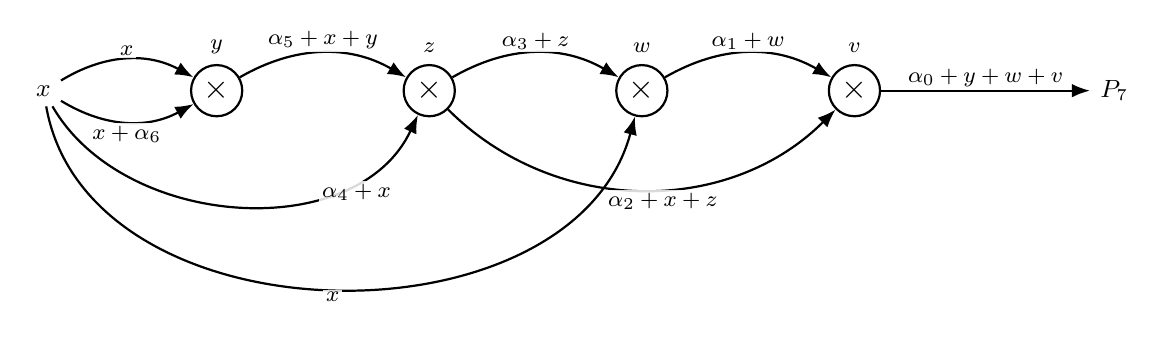
\begin{tikzpicture}[
    >=Latex, thick,
    mul/.style={circle, draw, inner sep=1.5pt, minimum size=6.5mm, font=\large, fill=white},
    inp/.style={font=\small},
    lbl/.style={font=\footnotesize, inner sep=1pt, fill=white, fill opacity=0.85, text opacity=1}
  ]
  \node[inp] (x) at (0,0) {$x$};
  \node[mul] (my) at (2.2,0) {$\times$};
  \node[mul] (mz) at (4.9,0) {$\times$};
  \node[mul] (mw) at (7.6,0) {$\times$};
  \node[mul] (mv) at (10.3,0) {$\times$};
  \node[inp] (out) at (13.6,0) {$P_7$};
  \node[font=\footnotesize] at (2.2,0.55) {$y$};
  \node[font=\footnotesize] at (4.9,0.55) {$z$};
  \node[font=\footnotesize] at (7.6,0.55) {$w$};
  \node[font=\footnotesize] at (10.3,0.55) {$v$};

  % y = x (x + a6)
  \draw[->] (x) to[bend left=30] node[lbl, above] {$x$} (my);
  \draw[->] (x) to[bend right=30] node[lbl, below] {$x+\alpha_6$} (my);
  % z = (a5 + x + y)(a4 + x)
  \draw[->] (my) to[bend left=30] node[lbl, above] {$\alpha_5+x+y$} (mz);
  \draw[->] (x) to[out=-60, in=-115, looseness=1.0] node[lbl, pos=0.78, below] {$\alpha_4+x$} (mz);
  % w = (a3 + z) x
  \draw[->] (mz) to[bend left=30] node[lbl, above] {$\alpha_3+z$} (mw);
  \draw[->] (x) to[out=-80, in=-105, looseness=1.05] node[lbl, pos=0.5, below] {$x$} (mw);
  % v = (a2 + x + z)(a1 + w)
  \draw[->] (mw) to[bend left=30] node[lbl, above] {$\alpha_1+w$} (mv);
  \draw[->] (mz) to[out=-45, in=-135, looseness=1.0] node[lbl, pos=0.55, below] {$\alpha_2+x+z$} (mv);
  % output: a0 + y + w + v
  \draw[->] (mv) -- node[lbl, above] {$\alpha_0+y+w+v$} (out);
  % Use the visible ink extent, not the lower Bezier control points.
  % This changes layout only: no clipping path is installed.
  \pgfresetboundingbox
  \path[use as bounding box] (-0.2,-2.9) rectangle (13.9,0.8);
\end{tikzpicture}
}
  \caption{The four-multiplication circuit for the septic base $P_7$ of \Cref{lem:septic-base}.
  Every multiplication gate takes two affine combinations of $x$ and previously computed values; the seven parameters $\alpha_0,\ldots,\alpha_6$ enter only as constant terms of these affine forms.}
  \label{fig:septic-circuit}
\end{figure}

\begin{proof}
\Cref{fig:septic-circuit} draws the circuit.
Write
\[
  P_7=x^7+c_6x^6+c_5x^5+c_4x^4+c_3x^3+c_2x^2+c_1x+c_0
\]
and write $z=x^3+z_2x^2+z_1x+z_0$.  The following triangular procedure
recovers the parameters from $(c_0,\ldots,c_6)$:
\begin{align}
 z_2&=c_6/2,\\
 z_1&=(c_5-z_2^2-1)/2,\\
 R&=c_4-1-2z_2z_1-z_2,\\
 \alpha_1&=c_3-z_2-z_2R-z_1^2-z_1,\\
 W&=c_2-z_1-1-z_2\alpha_1-z_1R,\\
 \alpha_6&=c_1-(z_1+1)\alpha_1-W(R+1-W),\\
 \alpha_4&=z_2-1-\alpha_6,\\
 \alpha_5&=z_1-\alpha_4(1+\alpha_6),\\
 z_0&=\alpha_4\alpha_5,\\
 \alpha_3&=W-z_0,\\
 \alpha_2&=R-2z_0-\alpha_3,\\
 \alpha_0&=c_0-(z_0+\alpha_2)\alpha_1.
\end{align}
Indeed, direct expansion gives
\[
 z_2=\alpha_4+1+\alpha_6,\qquad
 z_1=\alpha_4(1+\alpha_6)+\alpha_5,\qquad
 z_0=\alpha_4\alpha_5,
\]
while the coefficient equations for $P_7$ give, successively,
$R=2z_0+\alpha_2+\alpha_3$ and $W=z_0+\alpha_3$ and then the displayed
formulas for $\alpha_1$ and $\alpha_6$.
Substitution recovers every parameter.  The only division is by~$2$, which
is valid under the characteristic assumption.
\end{proof}


\subsubsection{Degree $15$}
\begin{algorithm}[H]
    \caption{
        Seven-product compatible joint realization in degree $15$.
    }

    \begin{algorithmic}
        \State $H_2[\alpha_6, \alpha_7](x) = (x + \alpha_7)x + \alpha_6$
        \State $H_4[\alpha_4, \alpha_5, \alpha_6, \alpha_7](x) = (H_2 + (x + \alpha_5))(H_2 - (x + \alpha_5)) + \alpha_4$
        \\
        \State $S^{(1)}_1 = Q_7[\alpha_8, \ldots, \alpha_{14}](x, H_2, H_4)$
        \State $S^{(1)}_2 = H_2 + \alpha_{3}$
        \State $S^{(1)}_3 = \alpha_1$
        \State $T^{(1)}_{15}[\alpha_0, \ldots, \alpha_{14}](x)
            = (S^{(1)}_1 + S^{(1)}_2)(S^{(1)}_1 - S^{(1)}_2) + S^{(1)}_3
            = (S^{(1)}_1)^2 - (S^{(1)}_2)^2 + S^{(1)}_3$
        \\
        \State $S^{(2)}_1 = H_4$
        \State $S^{(2)}_2 = H_2 + \alpha_2$
        \State $S^{(2)}_3 = \alpha_0$
        \State $T^{(2)}_{15}[\alpha_0, \ldots, \alpha_{14}](x)
            = (S^{(2)}_1 + S^{(2)}_2)(S^{(2)}_1 - S^{(2)}_2) + S^{(2)}_3 + T^{(1)}_{15}
            = (S^{(2)}_1)^2 - (S^{(2)}_2)^2 + S^{(2)}_3 + T^{(1)}_{15}$

        \State \begin{align}
            P_{15}[\alpha_0, \ldots, \alpha_{14}](x)
            &= x T^{(1)}_{15} + T^{(2)}_{15}
            \\&= (x+1)T^{(1)}_{15} + H_4^2 - (H_2 + \alpha_2)^2 + \alpha_0
        \end{align}
    \end{algorithmic}
\end{algorithm}

\subsubsection{Degree $27$}
\begin{algorithm}[H]
    \caption{
        Thirteen-product compatible joint realization in degree $27$.
    }

    \begin{algorithmic}
        \State $H_2[\alpha_2, \alpha_3](x) = (x + \alpha_3)x + \alpha_2$
        \\
        \State $S^{(1)}_1 = Q_{13}[\alpha_{14}, \ldots, \alpha_{26}](x, H_2)$ \Comment{This call records the quartic $H_4$.}
        \State $S^{(1)}_2 = Q_3[\alpha_4, \ldots, \alpha_6](x, H_2)$
        \State $S^{(1)}_3 = \alpha_1$
        \State $T^{(1)}_{27}[\alpha_0, \ldots, \alpha_{26}](x)
            = (S^{(1)}_1 + S^{(1)}_2)(S^{(1)}_1 - S^{(1)}_2) + S^{(1)}_3
            = (S^{(1)}_1)^2 - (S^{(1)}_2)^2 + S^{(1)}_3$
        \\
        \State $S^{(2)}_1 = Q_7[\alpha_7, \ldots, \alpha_{13}](x, H_2, H_4)$
        \State $S^{(2)}_2 = H_2$
        \State $S^{(2)}_3 = \alpha_0$
        \State $T^{(2)}_{27}[\alpha_0, \ldots, \alpha_{26}](x)
            = (S^{(2)}_1 + S^{(2)}_2)(S^{(2)}_1 - S^{(2)}_2) + S^{(2)}_3 + T^{(1)}_{27}
            = (S^{(2)}_1)^2 - (S^{(2)}_2)^2 + S^{(2)}_3 + T^{(1)}_{27}$

        \State \begin{align}
            P_{27}[\alpha_0, \ldots, \alpha_{26}](x)
            &= x T^{(1)}_{27} + T^{(2)}_{27}
            \\&= (x+1)T^{(1)}_{27} + (S^{(2)}_1)^2 - H_2^2 + \alpha_0
        \end{align}
    \end{algorithmic}
\end{algorithm}

\subsubsection{Degree $31$}
\begin{algorithm}[H]
    \caption{
        Fifteen-product compatible joint realization in degree $31$.
    }

    \begin{algorithmic}
        \State $H_2[\alpha_6, \alpha_7](x) = (x + \alpha_7)x + \alpha_6$
        \State $H_4[\alpha_4, \alpha_5, \alpha_6, \alpha_7](x) = (H_2 + (x + \alpha_5))(H_2 - (x + \alpha_5)) + \alpha_4$
        \\
        \State $S^{(1)}_1 = \bar Q_{15}[\alpha_{16}, \ldots, \alpha_{30}](x, H_2, H_4)$
        \State $S^{(1)}_2 = Q_7[\alpha_8, \ldots, \alpha_{14}](x, H_2, H_4)$
        \State $S^{(1)}_3 = Q_3[\alpha_1, \alpha_2, \alpha_3](x, H_2)$
        \State $T^{(1)}_{31}[\alpha_0, \ldots, \alpha_{30}](x)
            = (S^{(1)}_1 + S^{(1)}_2)(S^{(1)}_1 - S^{(1)}_2) + S^{(1)}_3
            = (S^{(1)}_1)^2 - (S^{(1)}_2)^2 + S^{(1)}_3$
        \\
        \State $S^{(2)}_1 = S^{(1)}_1 + \alpha_{15}$
        \State $S^{(2)}_2 = H_4$
        \State $S^{(2)}_3 = \alpha_0$
        \State $T^{(2)}_{31}[\alpha_0, \ldots, \alpha_{30}](x)
            = (S^{(2)}_1 + S^{(2)}_2)(S^{(2)}_1 - S^{(2)}_2) + S^{(2)}_3
            = (S^{(2)}_1)^2 - (S^{(2)}_2)^2 + S^{(2)}_3$

        \State \begin{align}
            P_{31}[\alpha_0, \ldots, \alpha_{30}](x)
            &= x T^{(1)}_{31} + T^{(2)}_{31}
            \\&= x(S^{(1)}_1)^2 + (S^{(1)}_1 + \alpha_{15})^2 - x(S^{(1)}_2)^2 - H_4^2 + x S^{(1)}_3 + \alpha_0
        \end{align}
    \end{algorithmic}
\end{algorithm}

\begin{figure}[H]
  \centering
  \resizebox{\textwidth}{!}{% Shell decomposition of the three finite splittable constructions.
\begin{tikzpicture}[x=1cm,y=1cm,>=Latex]
  \draw[fp decode] (0,6.25) -- node[fp label, above] {descending coefficient degree}
    (13.55,6.25);
  \node[fp label, anchor=east] at (0,6.25) {high};
  \node[fp label, anchor=west] at (13.55,6.25) {low};

  \node[fp panel title] at (0,5.72) {$n=15$};
  \node[fp active, minimum width=38mm, anchor=west] (a15) at (0,5.02)
    {recover $A=Q_7$\\from $(x+1)A^2$};
  \node[fp seam, minimum width=8mm, anchor=west] at (3.8,5.02) {$+1$};
  \node[fp second, minimum width=39mm, anchor=west] (h15) at (4.6,5.02)
    {recover $H_4$, then $H_2$\\from four rows};
  \node[fp seam, minimum width=17mm, anchor=west] at (8.5,5.02)
    {$-1$\\$-(2b+2)$};
  \node[fp recursive, minimum width=30mm, anchor=west] (l15) at (10.2,5.02)
    {solve $U,V,\alpha_1,\alpha_0$\\from the bottom rows};
  \node[fp label, anchor=west] at (0.35,4.4)
    {decode the parameters inside $A$ only after $H_2,H_4$ are known};

  \node[fp panel title] at (0,3.87) {$n=27$};
  \node[fp active, minimum width=31mm, anchor=west] (a27) at (0,3.17)
    {$A=Q_{13}$\\$(x+1)A^2$};
  \node[fp seam, minimum width=8mm, anchor=west] at (3.1,3.17) {$+1$};
  \node[fp second, minimum width=25mm, anchor=west] (c27) at (3.9,3.17)
    {$C=Q_7$\\$C^2$};
  \node[fp seam, minimum width=8mm, anchor=west] at (6.4,3.17) {$-1$};
  \node[fp pivot, minimum width=25mm, anchor=west] (b27) at (7.2,3.17)
    {$B=Q_3$\\$(x+1)B^2$};
  \node[fp seam, minimum width=8mm, anchor=west] at (9.7,3.17) {$+1$};
  \node[fp recursive, minimum width=30mm, anchor=west] (h27) at (10.5,3.17)
    {recover $H_2,s,r$\\then decode $A,C,B$};
  \draw[fp dependence] (h27.south) to[bend left=16]
    node[fp label, below] {$A$ supplies $H_4$ for $C$} (c27.south);

  \node[fp panel title] at (0,2.02) {$n=31$};
  \node[fp active, minimum width=35mm, anchor=west] (a31) at (0,1.32)
    {$A=\bar Q_{15}$ and shift $s$\\outer square gadget};
  \node[fp seam, minimum width=8mm, anchor=west] at (3.5,1.32) {$-1$};
  \node[fp second, minimum width=27mm, anchor=west] (b31) at (4.3,1.32)
    {$B=Q_7$\\$xB^2$};
  \node[fp seam, minimum width=8mm, anchor=west] at (7.0,1.32) {$+1$};
  \node[fp pivot, minimum width=22mm, anchor=west] (h31) at (7.8,1.32)
    {$H_4$\\$H_4^2$};
  \node[fp seam, minimum width=8mm, anchor=west] at (10.0,1.32) {$-1$};
  \node[fp recursive, minimum width=28mm, anchor=west] (c31) at (10.8,1.32)
    {$C=Q_3$, then $r$\\low residual};
  \node[fp label, anchor=west] at (4.0,0.56)
    {reconstruct $H_2$ from $H_4$, then discharge all conditional decoders};
  \node[fp label, anchor=west, text=fpBlue!80!black] at (0,-0.03)
    {Subtract the red boundary contributions before the corresponding pivot; $b$ is already known at its seam.};
\end{tikzpicture}
}
  \caption{The three finite decoders in one visual template.  A coloured
  block denotes a monic polynomial recovered from the indicated square
  window; each red seam is a fixed boundary coefficient contributed by the
  next block.  Recovering a polynomial and decoding its internal parameters
  are deliberately separated: the lower annotations show when the required
  powers have finally become available and the corresponding conditional
  decoder may be discharged.}
  \label{fig:special-case-decoders}
\end{figure}

\begin{lemma}[Finite cost bases]\label{lem:special-cases-splittable}
    For each $n\in\{15,27,31\}$, over an $n$-admissible field the
    special-case construction for $n$ produces a splittable pair.
    Moreover, the direct descending decoders below give the required
    compatibility windows for these three finite constructions; no general
    composition result is needed.  The two components have a joint
    $(n-1)/2$-realization that records their monic quadratic and quartic
    byproducts.
    In particular, $P_{15}$, $P_{27}$, and $P_{31}$ are decodable.
\end{lemma}
\begin{proof}
    We give the finite decoders explicitly.  Write
    $\Phi_n=xT^{(1)}_n+T^{(2)}_n=P_n$ and $G_n=\rng n$.
    For any polynomial $W$ write $W_j=\coeff{W}{j}$, so
    $p_j=\coeff{\Phi_n}{j}$.  Every square root below is the descending
    monic-square recursion (so it uses only divisions by $2$), and all
    quantities described as \text{known} are coefficients of the displayed
    auxiliary powers or quantities recovered in an earlier row block.
    To make explicit why only the top half of a square is needed, if
    $W=x^e+\sum_{r<e}w_rx^r$, then
    \[
      \coeff{W^2}{2e-s}
        =2w_{e-s}+\sum_{r=1}^{s-1}w_{e-r}w_{e-(s-r)}
        \qquad(1\le s\le e).
    \]
    Thus the coefficients in degrees $2e,\ldots,e$ recover the monic
    polynomial $W$ successively.

    \paragraph{The degree-$15$ construction.}
    Put
    \[
      A=S^{(1)}_1,\quad H_2=x^2+bx+c,\quad
      U=H_2+\alpha _3=x^2+bx+d_3,\quad
      V=H_2+\alpha _2=x^2+bx+d_2,
    \]
    and write $H_4=x^4+h_3x^3+h_2x^2+h_1x+h_0$.  The identity
    \[
      P_{15}=(x+1)A^2+H_4^2-(x+1)U^2-V^2+(x+1)\alpha _1+\alpha _0
    \]
    is a relative square shell with $M=x+1$, $\deg A=7$, and error
    \[
      E_A=H_4^2-(x+1)U^2-V^2+(x+1)\alpha_1+\alpha_0.
    \]
    Here $\deg E_A\le8$ and $[x^8]E_A=1$.  Hence
    \Cref{lem:relative-square-shell} recovers $A$ from the top block, with
    the displayed $+1$ seam correction.  Set
    $R=\Phi_{15}-(x+1)A^2$.  Its next four
    coefficients give
    \[
      h_3=R_7/2,\qquad b=h_3/2,\qquad
      h_2=(R_6-h_3^2)/2,
    \]
    \[
      h_1=(R_5+1-2h_3h_2)/2,\qquad
      h_0=(R_4+2b+2-h_2^2-2h_3h_1)/2.
    \]
    The defining relation $H_4=H_2^2-(x+\alpha _5)^2+\alpha _4$
    then yields
    \[
      c=(h_2-b^2+1)/2,\quad
      \alpha _5=bc-h_1/2,\quad \alpha _4=h_0-c^2+\alpha _5^2.
    \]
    Finally put $R'=R-H_4^2$.  The four bottom equations are
    \[
      \begin{aligned}
      d_3&=-(R'_3+b^2+4b)/2,\\
      d_2&=-(R'_2+2b^2+2d_3+2bd_3)/2,\\
      \alpha _1&=R'_1+2bd_3+d_3^2+2bd_2,\\
      \alpha _0&=R'_0+d_3^2+d_2^2-\alpha _1.
      \end{aligned}
    \]
    Hence $\alpha _3=d_3-c$ and $\alpha _2=d_2-c$.  Once $H_2,H_4$
    are known, the unitriangular decoder for $Q_7$ (\Cref{lem:Q-unitriangular})
    recovers the parameters inside $A$; the side information is discharged
    by \Cref{lem:discharge-side-information} because $A,H_2,H_4$ have all
    been recovered from $P_{15}$.

    \paragraph{The degree-$27$ construction.}
    Write
    \[
      A=S^{(1)}_1,\quad C=S^{(2)}_1,\quad B=S^{(1)}_2,
      \quad H_2=x^2+ux+v,
    \]
    where $\deg A=13$, $\deg C=7$, and $\deg B=3$, and put
    $s=\alpha _1$ and $r=\alpha _0$.  The identity
    \[
      P_{27}=(x+1)A^2-(x+1)B^2+(x+1)s+C^2-H_2^2+r
    \]
    gives three consecutive relative square shells.  First set
    \[
      E_A=-(x+1)B^2+(x+1)s+C^2-H_2^2+r.
    \]
    Since $\deg E_A\le14$ and $[x^{14}]E_A=1$,
    \Cref{lem:relative-square-shell} with $M=x+1$ recovers $A$.  Set
    $R=\Phi_{27}-(x+1)A^2$.  Then
    \[
      R=C^2+E_C,\qquad
      E_C=-(x+1)B^2+(x+1)s-H_2^2+r,
    \]
    where $\deg E_C\le7$ and $[x^7]E_C=-1$.  The same lemma, now with
    $M=1$, recovers $C$.  Set $R'=R-C^2=E_C$.  After changing sign,
    \[
      -R'=(x+1)B^2+E_B,\qquad
      E_B=-(x+1)s+H_2^2-r,
    \]
    with $\deg E_B\le4$ and $[x^4]E_B=1$.  A third application with
    $M=x+1$ recovers $B$.  These are exactly the seams $+1,-1,+1$ in
    \Cref{fig:special-case-decoders}.  Finally, with
    $L=R'+(x+1)B^2=(x+1)s-H_2^2+r$, we have
    \[
      u=-L_3/2,\qquad v=-(L_2+u^2)/2,\qquad
      s=L_1+2uv,\qquad r=L_0+v^2-s.
    \]
    Decode $A=Q_{13}$ first using the recovered $H_2$; by
    \Cref{lem:Q4k+1-from-H2} this also reconstructs the quartic $H_4$ used
    by $C$.  Then decode $C=Q_7$ from $(H_2,H_4)$ and $B=Q_3$ from $H_2$.
    These three decoders recover their respective parameter blocks without
    assuming an internal power before it has been reconstructed; this is
    exactly the substitution in \Cref{lem:discharge-side-information}.

    \paragraph{The degree-$31$ construction.}
    Put
    \[
      A=S^{(1)}_1,\quad B=S^{(1)}_2,\quad C=S^{(1)}_3,
      \quad H=H_4,
    \]
    with degrees $15,7,3,4$, respectively, and set
    $s=\alpha _{15}$ and $r=\alpha _0$.  Since
    \[
      P_{31}=xA^2+(A+s)^2+E,
      \qquad E=-xB^2-H^2+xC+r,
    \]
    we have $\deg E\le15=\deg A$ and $[x^{15}]E=-1$.  Therefore
    \Cref{lem:square-gadget-boundary} recovers $A$ and $s$ directly, with
    the displayed fixed boundary correction.  Set
    \[
      R'=\Phi_{31}-xA^2-(A+s)^2.
    \]
    The remaining two monic blocks are again relative square shells:
    \[
      -R'=xB^2+E_B,\qquad E_B=H^2-xC-r.
    \]
    Here $\deg E_B\le8$ and $[x^8]E_B=1$, so
    \Cref{lem:relative-square-shell} with $M=x$ recovers $B$.  Put
    $R''=R'+xB^2$.  Then
    \[
      -R''=H^2+E_H,\qquad E_H=-xC-r,
    \]
    with $\deg E_H\le4$ and $[x^4]E_H=-1$.  The same lemma with $M=1$
    recovers $H$.  The remaining polynomial
    $R'''=R''+H^2=xC+r$ gives
    $r=R'''_0$ and $C=(R'''-r)/x$.  If
    $H=x^4+h_3x^3+h_2x^2+h_1x+h_0$, its parameter block is
    \[
      \alpha _7=h_3/2,\quad
      \alpha _6=(h_2-\alpha _7^2+1)/2,\quad
      \alpha _5=\alpha _7\alpha _6-h_1/2,\quad
      \alpha _4=h_0-\alpha _6^2+\alpha _5^2.
    \]
    The previously proved decoders for $Q_3,Q_7,\bar Q_{15}$ (the latter
    given $(H_2,H_4)$) recover all remaining parameters.  Formally,
    \Cref{lem:discharge-side-information} substitutes the recovered
    $H_2,H_4$ into these conditional decoders.

    It remains to record causality.  The preceding formulas have the following
    row shifts; $t$ denotes a coefficient degree inside the recovered
    polynomial.
    \[
    \begin{array}{c|c|c}
      n&\text{recovered quantity}&\text{row where its coefficient is read}\\ \hline
      15&[x^t]A,\ [x^t]H_4,\
          (\alpha_3,\alpha_2,\alpha_1,\alpha_0)
        &p_{t+8},\ p_{t+4},\ (p_3,p_2,p_1,p_0)\\
      27&[x^t]A,\ [x^t]C,\ [x^t]B,\ (H_2,s,r)
        &p_{t+14},\ p_{t+7},\ p_{t+4},\ (p_3,\ldots,p_0)\\
      31&[x^t]A,\ s,\ [x^t]B,\ [x^t]H_4,\ [x^t]C,\ r
        &p_{t+16},\ p_{15},\ p_{t+8},\ p_{t+4},\ p_{t+1},\ p_0
    \end{array}
    \]
    At a shared boundary the only contribution from the next block is the
    displayed monic coefficient $1$ or $-1$, which is subtracted before that
    block is entered (in the $31$ case this includes the row-$4$ correction
    for $xC$).

    Maintain the descending invariant that a quantity first solved in row
    $r$ is a polynomial in the observed rows $p_s$ with $s\ge r$ and in
    quantities solved above it.  Every displayed square or Cauchy recurrence
    has this form, so the invariant holds across all boundary rows.  The row
    shifts in the table then show that $[x^j]T^{(1)}$ uses only $p_i$ with
    $i\ge j+1$, whereas $[x^j]T^{(2)}$ uses only $p_i$ with $i\ge j$.
    These are exactly the cutoffs in \Cref{def:compatible-pair}.  Since the
    leading coefficient $p_n=1$ is fixed, all three pairs are compatible on
    $\rng n$, hence splittable, and their combined polynomials are decodable.

    Finally, the displayed algorithms are joint circuits for the two
    components.  Charging each shared intermediate only once gives
    \[
    \begin{array}{c|c|c}
      n&\text{products in the joint realization}&\text{total}\\ \hline
      15&H_2:1,\ H_4:1,\ Q_7:3,\ \text{two outer products}:2&7\\
      27&H_2:1,\ Q_{13}:6,\ Q_3:1,\ Q_7:3,\ \text{two outer products}:2&13\\
      31&H_2,H_4:2,\ \bar Q_{15}:7,\ Q_7:3,\ Q_3:1,\
          \text{two outer products}:2&15.
    \end{array}
    \]
    The $Q_{13}$ call in degree~$27$ records the required $H_4$; in the
    other two cases $H_2,H_4$ are displayed intermediates.  Hence all three
    realizations record both byproducts and have exactly $(n-1)/2$ products.
\end{proof}


\subsection{Final construction and decoder}
\label{sec:final}

All ingredients are now in place.  The final recursion uses the known-powers
gadgets $Q_{2^t-1}$, the fill gadget $A_{2^l}$, the $T_{k,2^l}$ remainder
recursion, and the three causal closure operations.  Each recursive branch
comes with its own cutoff-respecting decoder: the closure lemmas handle local
combinations, and the stage tables handle $T$.  The decoder summaries used
below are
\Cref{alg:decode-Q-2kminus1} for $Q_{2^t-1}$,
\Cref{alg:decode-fill} for $A_{2^l}$,
and \Cref{alg:decode-Rk2l} for the combined remainder polynomial used in the $T_{k,2^l}$ recursion;
they assemble into \Cref{alg:final-decoder}.  The schedules certified in
Lean substitute the peeled gadget $Q^{\mathrm{peel}}$ (\Cref{sec:peeled-Q})
for every known-powers instance; \Cref{thm:construction-height-peeled}
records the resulting $O(\log n)$ height at the identical gate ledger.
\Cref{fig:final-recursion} charts the routing of the strong induction.

\begin{figure}[H]
  \centering
  \resizebox{\textwidth}{!}{% Routing diagram for the strong induction and the final multiplication.
\begin{tikzpicture}[x=1cm,y=1cm,>=Latex]
  \node[fp active, rounded corners, minimum width=30mm, minimum height=8mm]
    (n) at (6.75,5.2) {odd target degree $n\ge3$};

  \node[fp known, rounded corners, minimum width=19mm] (seven) at (0.9,3.75)
    {$n=7$\\direct septic};
  \node[fp second, rounded corners, minimum width=30mm] (bases) at (3.45,3.75)
    {$3$ base; $15$ fused $k=1$\\$27,31$ septic bridges};
  \node[fp active, rounded corners, minimum width=23mm] (one) at (6.35,3.75)
    {$n\equiv1\pmod4$\\$T_{2k,2}$ crown};
  \node[fp active, rounded corners, minimum width=23mm] (three) at (9.05,3.75)
    {$n\equiv3\pmod8$\\$8k+3$ shell};
  \node[fp active, rounded corners, minimum width=23mm] (sevenmod) at (11.85,3.75)
    {$n\equiv7\pmod8$\\$8k+7$ shells};

  % Route through one branch bus: the five cases are mutually exclusive, and
  % the common trunk avoids the visually misleading crossings of five curves.
  \coordinate (route) at (6.75,4.55);
  \draw[line width=.65pt, draw=black!75] (n.south) -- (route)
    -- (0.9,4.55) -- (11.85,4.55);
  \draw[fp flow] (0.9,4.55) -- (seven.north);
  \draw[fp flow] (3.45,4.55) -- (bases.north);
  \draw[fp flow] (6.35,4.55) -- (one.north);
  \draw[fp flow] (9.05,4.55) -- (three.north);
  \draw[fp flow] (11.85,4.55) -- (sevenmod.north);

  \node[fp recursive, rounded corners, minimum width=28mm] (small3) at (8.75,2.1)
    {smaller pair at\\$m=(n+1)/4$};
  \node[fp recursive, rounded corners, minimum width=28mm] (small7) at (11.95,2.1)
    {smaller pair at\\$m=(n-3)/4$};
  \draw[fp flow] (small3.north) -- node[fp label, right] {insert} (three.south);
  \draw[fp flow] (small7.north) -- node[fp label, right] {insert} (sevenmod.south);
  \node[fp label, anchor=west] at (8.0,1.4)
    {$m<n$, and the explicit exceptions ensure $m\ne7$};

  \node[fp recursive, minimum width=73mm, minimum height=7mm] (pair) at (4.2,0.55)
    {shared construction of $(T_n^{(1)},T_n^{(2)})$: $(n-1)/2$ products};
  \node[fp gate] (mul) at (8.65,0.55) {$\times$};
  \node[fp active, minimum width=34mm, minimum height=7mm] (out) at (11.3,0.55)
    {$P_n=xT_n^{(1)}+T_n^{(2)}$\\$(n+1)/2$ products total};
  \node[fp label, below=1mm of mul] {multiply by $x$};
  \draw[fp flow] (pair.east) -- (mul.west);
  \draw[fp flow] (mul.east) -- (out.west);
\end{tikzpicture}
}
  \caption{Routing of the final strong induction.  The $4k+1$ branch closes
  directly through the $T$ recursion.  The other two congruence classes wrap
  a strictly smaller compatible pair in one or two square shells.  The
  exceptional list removes exactly the cost-optimal recursive calls that
  would otherwise land at the missing three-product degree-$7$ realization
  (and the degree-$15$ byproduct mismatch).
  The bottom row separates the cost of constructing the shared pair from the
  final multiplication by~$x$.  All known-powers instances inside these
  branches are scheduled as the peeled $Q^{\mathrm{peel}}$
  (\Cref{thm:construction-height-peeled}), giving height
  $2\lceil\log_2 n\rceil+4$ for the odd degrees charted here (the even
  lift of \Cref{thm:construction-count} adds one).}
  \label{fig:final-recursion}
\end{figure}

\begin{algorithm}[H]
  \caption{Final odd-degree construction}\label{alg:final-construction}
  \begin{algorithmic}
    \Require odd integer $n\ge 3$
    \Ensure a decodable monic polynomial $P_n$; if $n\ne7$, also a
    jointly $(n-1)/2$-realized splittable pair
    $(T^{(1)}_n,T^{(2)}_n)$ that is compatible with no auxiliary data and
    records the required power byproducts

    \If{$n=7$}
      \State Use the direct septic construction in \Cref{lem:septic-base}.
    \ElsIf{$n\in\{3,15,27,31\}$}
      \State Use the explicit special-case constructions in \Cref{sec:special-cases}.
    \ElsIf{$n\equiv 1\pmod 4$}
      \State Write $n=4k+1$ and construct $(T^{(1)}_{4k+1},T^{(2)}_{4k+1})$ via the $T_{2k,2}$ call; see \Cref{lem:4k+1-splittable}.
    \ElsIf{$n\equiv 3\pmod 8$}
      \State Write $n=8k+3$ and extend the smaller compatible joint realization for $2k+1$ by \Cref{alg:constr-8k+3}.
    \Else
      \State Write $n=8k+7$ with $k\ge 2$ and extend the smaller compatible joint realization for $2k+1$ by \Cref{alg:constr-8k+7} (using $\bar Q_{15}$ or $\bar Q_{8k+7}$ as needed).
    \EndIf
  \end{algorithmic}
\end{algorithm}

\begin{algorithm}[H]
  \caption{Final decoder for $P_n$ (structural recursion)}\label{alg:final-decoder}
  \begin{algorithmic}
    \Require odd $n\ge 3$ and $P_n$ produced by \Cref{alg:final-construction}.
      For the peeled schedules of \Cref{thm:construction-height-peeled}, every
      invocation of \Cref{alg:decode-Q-2kminus1} below is replaced by the
      decoder of \Cref{lem:peeled-Q-decodable}, which has the identical
      interface.
    \Ensure the full parameter list $(\alpha_0,\ldots,\alpha_{n-1})$

    \If{$n=7$}
      \State Apply the triangular decoder in \Cref{lem:septic-base}.
    \ElsIf{$n\in\{3,15,27,31\}$}
      \State Decode by the explicit special-case proofs in \Cref{sec:special-cases}.
    \ElsIf{$n\equiv 1\pmod 4$}
      \State Write $n=4k+1$.
      \State Use the five top-coefficient pivots in \Cref{lem:4k+1-splittable} to derive $H_2,H_4,\tilde H_4=H_4+\rho$ and the five outer parameters.
      \State Derive the pair $(U,V)=T_{k,4}(x,H_2,H_4,\tilde H_4)$ from $P_{4k+1}=xU+V$ using the cutoff decoder in \Cref{lem:4k+1-splittable}.
      \State Form $x(U-H_4^k)+(V-\tilde H_4^k)$ and apply \Cref{alg:decode-Rk2l} at $(k,l)=(k,2)$ to extract $\alpha_0,\ldots,\alpha_{4k-5}$.
    \ElsIf{$n\equiv 3\pmod 8$}
      \State Write $n=8k+3$ and apply the square-gadget extraction in \Cref{lem:8k+3-splittable} to recover the auxiliary polynomials and the squared smaller pair.
      \State Recover $P_{2k+1}$ by monic square roots and recurse on it; this reconstructs $H_2$.
      \State Decode $S^{(1)}_2=Q_{4k+1}$ first via \Cref{lem:Q4k+1-from-H2}, which reconstructs $H_4$; only then decode $S^{(1)}_3=\mathcal Q_{2k-1}$ by the dispatch of \Cref{lem:odd-gadgets-H2H4}, with \Cref{alg:decode-Q-2kminus1} for nested Mersenne blocks.
    \Else
      \State Write $n=8k+7$ with $k\ge 2$ and apply the two square-gadget extractions in \Cref{lem:8k+7-splittable}; this recovers both auxiliary polynomials and isolates $P_{2k+1}$.
      \State Recurse on $P_{2k+1}$, thereby reconstructing the internal powers $H_2,H_4$.
      \State Only now decode the recovered auxiliary gadgets by the $\mathcal Q_d$ dispatch of \Cref{lem:odd-gadgets-H2H4} (i.e.\ \Cref{lem:Q4k+1-from-H2}, \Cref{lem:Q-odd-degree-with-powers}, or \Cref{lem:barQ15,lem:barQ8k+7}), with \Cref{alg:decode-Q-2kminus1} for nested Mersenne blocks.
    \EndIf
  \end{algorithmic}
\end{algorithm}

\begin{theorem}[Cost-optimal compatible pairs in odd degree]
\label{thm:odd-realizable-pairs}
    Let $n\ge3$ be odd with $n\ne7$, and assume that $\mathbb F$ is
    $n$-admissible.  Then there exists a splittable pair
    $(T^{(1)}_n,T^{(2)}_n)$ that is compatible on an explicit window with no
    auxiliary data and has a joint $(n-1)/2$-realization
    (\Cref{def:joint-realization}) of multiplicative height at most
    $2\lceil\log_2n\rceil+3$.  The realization
    records a monic quadratic $H_2$ and, when $n\ge5$, a monic quartic $H_4$.
    In particular, $P_n=xT^{(1)}_n+T^{(2)}_n$ is decodable.
\end{theorem}
\begin{proof}
    We argue by strong induction on odd $n$, proving simultaneously the
    asserted compatible-pair conclusion, the exact joint multiplication
    count, and the byproduct statement.  For the height conjunct, the ledger
    of \Cref{thm:construction-height-peeled} threaded through the same
    induction gives $2\lceil\log_2n\rceil+3$ along the pair branches (the
    bound $B(L)=2L+3$ there); the same constant is the height conjunct of
    the machine-checked Lean statement (\texttt{odd\_realizable\_pairs}) for
    the very circuit exhibited here (see the closing remark of
    \Cref{sec:peeled-Q}).
    Since $n$-admissibility implies $m$-admissibility for every $m<n$, all
    recursive pairs and auxiliary gadgets below satisfy their stated
    characteristic hypotheses over the same field.
    The strengthened induction invariant is that every constructed pair records
    its monic quadratic $H_2$ as a polynomial byproduct, and every constructed
    pair of degree at least five also records a monic quartic $H_4$.  These
    polynomials use no extra gates: they are intermediate values already
    displayed in the construction.  The degree-$3$ base records its $H_2$;
    the $4k+1$ and special constructions display both powers; the $8k+3$ step
    inherits $H_2$ and obtains $H_4$ as the byproduct of its
    $Q_{4k+1}(x,H_2)$ call; and the $8k+7$ step inherits both powers from its
    smaller pair.  Thus the byproduct invariant is preserved by every branch.

    Unconditional compatibility is stronger than decodability and is precisely what permits a
    smaller pair to be used before any powers internal to its construction have
    been reconstructed.  The direct proofs in
    \Cref{lem:4k+1-splittable,lem:8k+3-splittable,lem:8k+7-splittable}
    verify the cutoff formulas for each of the three recursive branches; no
    general composition assertion is used.

    The realizability assertion is carried by those same branches, not by a
    separate numerical recurrence.  In either odd induction step, execute the
    smaller joint circuit once, reuse its recorded $H_2,H_4$ wires as inputs
    to the auxiliary gadgets, and then form the two displayed
    difference-of-squares outputs.  Each difference of squares uses the one
    product $(S_3+S_2)(S_3-S_2)$ already shown in the construction algorithm.
    Thus the two output components share the smaller circuit and the power
    byproducts literally; the sums below count the gates of this one joint
    circuit.  The $4k+1$ and finite branches are already displayed as joint
    circuits in the same way.

    The finite cost bases have two distinct causes.  For $n=27$ and
    $n=31$, the relevant recursion would call degree~$7$.  Although the
    septic is algebraically splittable by \Cref{rem:canonical-split}, we do
    not have the three-product compatible joint realization, with recorded
    powers, required by either cost-optimal induction step.  For $n=15$, the smaller degree-$3$
    pair is compatible, but records only $H_2$, whereas the degree-$7$
    auxiliary gadget in the generic $8k+7$ step also requires $H_4$.
    Constructing that quartic separately would exceed the target count; the
    special degree-$15$ circuit instead replaces the generic $Q_3$ block by a
    scalar shift of $H_2$ and spends the saved product on $H_4$.  Thus these
    cases are not artifacts of the decoder proof.

    For $n\equiv 1\pmod 4$ and $n\ge 5$, write $n=4k+1$ and use
    \Cref{lem:4k+1-splittable}.  Its joint-realization clause gives exactly
    $2k=(n-1)/2$ products and records both powers.

    For $n\equiv 3\pmod 8$ we can write $n=8k+3$ with $k\ge 0$.
    If $k=0$ then $n=3$ is supplied by the compatible base
    \Cref{lem:base-three-compatible}.  Hence assume $k\ge1$.
    If $k=3$ then $n=27$ is covered, with its exact cost and recorded powers,
    by \Cref{lem:special-cases-splittable}.
    Otherwise $k\ne 3$, so $2k+1<n$ is odd and $2k+1\ne 7$; by the induction
    hypothesis we have a compatible joint realization for $2k+1$ costing
    $k$ products.  The full conclusion of \Cref{lem:8k+3-splittable} gives
    the required decoder, compatibility, recorded powers, and joint cost
    \[
       k+3k+1=4k+1=\frac{(8k+3)-1}{2}.
    \]

    For $n\equiv 7\pmod 8$ we can write $n=8k+7$ with $k\ge 0$.
    The case $k=0$ is exactly $n=7$ and is excluded.
    If $k=1$ then $n=15$, and if $k=3$ then $n=31$; both are covered, with
    their exact costs and recorded powers, by
    \Cref{lem:special-cases-splittable}.  Otherwise $k\ne1,3$, so $k\ge2$
    and $2k+1<n$ is odd with $2k+1\ne7$.  The induction hypothesis gives a
    compatible joint realization for $2k+1$ costing $k$ products, and
    the full conclusion of \Cref{lem:8k+7-splittable} gives the required
    decoder, compatibility, recorded powers, and joint cost
    \[
       k+3k+3=4k+3=\frac{(8k+7)-1}{2}.
    \]
    The byproduct discussion above verifies in each branch that these are
    realizations of the full strengthened invariant, completing the induction.
\end{proof}

\begin{theorem}[Exact multiplication count]\label{thm:construction-count}
    For every odd $n\ge3$ with $n\ne7$, the construction computes the
    splittable pair $(T^{(1)}_n,T^{(2)}_n)$ using exactly $(n-1)/2$
    multiplications, and therefore computes
    $P_n=xT^{(1)}_n+T^{(2)}_n$ using $(n+1)/2$ multiplications.  The direct
    septic construction uses four multiplications as well.  Consequently, over
    every $n$-admissible field, each monic degree-$n$ polynomial with $n\ge3$
    is covered by a decodable circuit using
    $\lfloor n/2\rfloor+1$ multiplications.
\end{theorem}
\begin{proof}
    For odd $n\ne7$, \Cref{thm:odd-realizable-pairs} supplies the joint
    $(n-1)/2$-realization and its decoder.  Multiplying $T^{(1)}_n$ by $x$
    once gives $P_n$ and raises the cost to $(n+1)/2$.  For $n=7$ the direct
    circuit in \Cref{lem:septic-base} already has the same cost, namely four.

    Finally, if $n\ge4$ is even, first use the odd construction for a monic
    degree-$(n-1)$ polynomial $Q$, at cost $n/2$, and output
    $c_0+xQ$, using one additional product.  This gives $n/2+1$ products.
    Its decoder first reads $c_0$ from the constant coefficient and then
    shifts the remaining coefficients down by one before invoking the decoder
    for $Q$, so this even lift is decodable.  Degrees $1$ and $2$ use
    $x+\alpha_0$ and $(x+\alpha_1)x+\alpha_0$, respectively, and are
    decodable with zero and one product.  Finally,
    \Cref{lem:polynomial-left-inverse-automorphism} turns each of these
    polynomial decoders into a two-sided polynomial preprocessing map.
    Hence the families cover every monic coefficient vector, as asserted.
\end{proof}

\begin{remark}[Exact characteristic restriction]
\label{rem:bad-primes}
    The hypothesis of $n$-admissibility in
    \Cref{thm:odd-realizable-pairs,thm:construction-count} is used only to
    invert the integers listed in \eqref{eq:bad-primes} along the routing
    of \Cref{alg:final-construction}.  Consequently both theorems hold
    verbatim, with the same circuits, the same decoder
    \Cref{alg:final-decoder}, the same multiplication count
    $\lfloor n/2\rfloor+1$ and the same height, over every field whose
    characteristic is not in $\mathrm{Bad}(n)$; equivalently, over every
    field in which each element of $\mathrm{Bad}(n)$ is a unit.  The set
    $\mathrm{Bad}(n)$ is computed by \texttt{tools/bad\_primes.py}, always
    contains~$2$ for $n\ge5$, and its odd elements are at most $(n-1)/4$,
    so characteristic zero or $p>n$ remains a uniform sufficient condition.
    For example $\mathrm{Bad}(n)=\{2\}$ for $5\le n\le12$ and for
    $n=15,17,19,23,31,33,35,39,47$, while $\mathrm{Bad}(13)=\{2,3\}$,
    $\mathrm{Bad}(21)=\{2,5\}$ and $\mathrm{Bad}(29)=\{2,3,7\}$: the
    degree-$47$ circuit is decodable over $\mathrm{GF}(3)$, whereas the
    degree-$13$ crown divides by $2k=6$.  The Lean statement
    \texttt{odd\_realizable\_pairs} certifies the uniform hypothesis that
    $1,\dots,n$ are units (\Cref{sec:formalization-map:units}); the sharper
    set $\mathrm{Bad}(n)$ is read off the displayed pivots and is not
    machine-checked.
\end{remark}






\end{document}
